\chapter*{Abstract}
\noindent
This thesis presents a first search for the fully leptonic decay \Bmumumu in any experiment. This search is performed using
proton-proton collision data at LHCb corresponding to an integrated luminosity of $4.7$ fb$^{-1}$. The search is carried out in the
region where the minimum of the two $\mumu$ mass combinations is below $980$\mevcc. From the theoretical point of view, the measurement of the branching fraction of decay is interesting given that the recent theoretical prediction \cite{Danilina:2018uzr} of the branching fraction for \Bmumumu of $1.3 \times 10^{-7}$ is high. Moreover, this decay is sensitive to the magnitude of the quark coupling strength between $b$ and $u$ quark, which is of great interest given that there are some tensions in measurements of this magnitude.

The data shows to be consistent with the background only hypothesis and the limit $1.4 \times 10^{-8}$ at 95\% confidence level is set on the branching fraction in the stated kinematic region. This is therefore not consistent with the theoretical prediction made in \cite{Danilina:2018uzr}.

This thesis also presents a study of the response of the detector if three muons pass through it. This study shows that correlations induced by a trimuon system in the detector are substantial and they need to be addressed properly.


%reports the branching fraction measurement of the rare Cabibbo-suppressed decay \Lbpi. The decay is observed for the first time with a $\SIG\sigma$ deviation from the background-only hypothesis. This is the first observation of a $b$\to$d$ quark transition in the baryon sector. The dataset used for the measurement corresponds to 3\:\invfb of \proton{}\proton collisions collected at the LHCb experiment at CERN. The branching fraction is measured using \Lb\to\jpsi(\to\mumu)\proton\pim as a normalisation channel and is measured as
%\begin{equation*}
%  \BF(\Lbpi) = \BFV,
%\end{equation*}
%where the first error is the statistical uncertainty, the second is the systematic uncertainty and the third is the uncertainty on $\BF(\Lbpijpsi)$.
%The measurement of $\BF(\Lbpi)$ can be combined with the branching fraction measurement for \LbK to give constraints on the ratio of CKM matrix elements $|\frac{\Vtd}{\Vts}|$. Such a determination of $|\frac{\Vtd}{\Vts}|$  requires a theory prediction for the ratio of the relevant form factors.

%This thesis also reports the ratio of tracking efficiencies, $\epsilon_{\mathrm{rel}}$, between data and simulation for $\KS\to\pip\pim$ decays occurring within the LHCb detector acceptance. As \KS particles are long-lived, their associated tracking efficiencies are less precisely determined compared to those of shorter-lived particles. The average value of $\epsilon_{\mathrm{rel}}$ for $\KS\to\pip\pim$ decays, where the \KS has a flight distance of $\gsim 1\m$, is found to be
%\begin{equation*}
%  \epsilon_{\mathrm{rel}} = 0.70\pm0.02.
%\end{equation*}

% To perform this calibration measurement a novel technique was developed which has the potential to be used in measuring the value of $\epsilon_{\mathrm{rel}}$ for other decays involving long-lived particles.

%The value of $\epsilon_{\mathrm{rel}}$ is found to be weakly dependent on the kinematics of the events as well as the particles decay position in the detector. 
\chapter{Introduction}
%The Standard Model is without question the most powerful and tested theory of particle physics. It describes and predicts many phenomena very well even though the theory is not including any explanation for the nature of dark matter and it doesn't make any attempt to describe gravity in a quantum field theory framework.

%Furthermore, fine-tuning of some parameters in the Standard Model such as the Higgs mass, where parameters get exactly the right value to produce required behaviour, beg questions if there is some symmetry in the model building that is missing. In this chapter, the theoretical basis of the Standard Model is discussed and is then followed by experimental and theoretical consideration of fully leptonic decays.


The field of particle physics aims to describe the universe we see today by decomposing everything into fundamental building blocks, which then exhibit certain behaviour according to a given set of rules. So far, the best theoretical formulation that describes the universe around us in form of these building blocks, the Standard Model (\Gls{SM}), was conceived last century. Some achievements of the \gls{SM} do really leave us breathless with agreement between theoretical and experimental results of ten parts in a billion. 

This theory is, however, incomplete as it fails to address several issues. The theory does not include any explanation for the nature of dark matter and it doesn't make any attempt to describe gravity in a quantum field theory framework. Furthermore, fine-tuning of some parameters in the \gls{SM} such as the Higgs mass, where parameters get exactly the right value to produce required behaviour, beg questions if there is some symmetry in the model building that is missing. Lastly, as with any model, the \gls{SM} operates with many free parameters that need to be plugged in so that predictions can be made. So why are there exactly so many?

This thesis describes a search for a decay which can help to shine light on some of these parameters and is organised as follows. In~\autoref{stheory} the \gls{SM} of particle physics is discussed together with the theoretical and experimental motivation for fully leptonic decays, especially for the \Bmumumu decay. In~\autoref{chap:dec} the tool to search for \Bmumumu decays, the LHCb detector, is detailed. Discussion about how a trimuon signature behaves in the detector is covered in~\autoref{chap:trimuon}. The analysis of \Bmumumu, the central theme for the thesis, is then described in three chapters:~\autoref{chap:sel}, where selection for signal and normalisation is given;~\autoref{chap:back}, where backgrounds to the \Bmumumu are considered; and finally~\autoref{chap:masandef}, where the efficiencies and mass fits are discussed. The result along with its implications will then close this thesis in~\autoref{chap:Results}.

\chapter{Theory}
\label{stheory}
%\subsection{Introduction to Mixing Phenomenology}
\textit{The Standard Model is without question the most powerful and tested theory of particle physics. It describes and predicts many phenomena very well even though as discussed in the previous chapter it fails to address certain known issues. In this chapter, the theoretical basis of the Standard Model is first laid out which is then followed by the experimental and theoretical considerations of fully leptonic decays. The introduction in this chapter is based on Ref\cite{Griffiths:111880},\cite{Novaes:1999yn} and \cite{Pich:2012sx}.}



\section{Review of the Standard Model}
The \gls{SM} of particle physics is currently the most accurate model describing the buildings blocks of matter, particles, and their interactions via forces. In particular the \gls{SM} describes all the fundamental forces but gravity. It is a quantum field theory (\gls{QFT}) whereby the dynamics of the system is captured by the most general renormalisable Lagrangian density that is invariant under gauge symmetry. \gls{QFT} considers particles to be excited states of an underlying field, also known as quanta. In the \gls{SM}, particles and forces are the results of interactions between scalar, vector and spinor fields. In general there are two sets of particles. The first set are force-carrying particles also known as bosons, which have integer spin and are quanta of the scalar and vector fields. More specifically, there is the Higgs boson, the only elementary scalar boson in the \gls{SM}, and vector bosons: gluons, $W^{\pm}$, Z and $\gamma$. Secondly, there are the non-force carrying particles, which are fermions, quanta of spinor fields. Unlike bosons they carry half-integer spin. These can be further classified into two elementary families of particles: quarks, which cannot be observed alone and leptons which can be detected on their own. Out of all of these fundamental particles, those that have mass acquire it by the Higgs mechanism.

%Quarks are affected by all three fundamental forces. They come in six different \textit{flavours} and they carry fractional charge as seen in~\autoref{nonlin}.

\begin{table}
\centering % used for centering table 
\begin{tabular}{c c c c} % centered columns (4 columns) 
\toprule %inserts double horizontal lines 
Generation & Flavour & Charge & Quark Mass \\ [0.5ex]\hline% inserts table 
%heading 
% inserts single horizontal line 
1st & up  \textit{u}& +2/3 & $2.2\bfrac{+0.6}{-0.4}$ \mev \\ % inserting body of the table 
1st & down \textit{d}& -1/3 & $4.7\bfrac{+0.5}{-0.4}$ \mev \\[1ex]
2nd & charm \textit{c}& +2/3 & $1.28\pm0.03$\gev\\
2nd & strange \textit{s}& -1/3 &  $96\bfrac{+8}{-4}$ \mev\\[1ex]
3rd & top \textit{t}& +2/3 &  $173.1\pm0.6$ \gev \\
3rd & bottom \textit{b}& -1/3 & $4.18\bfrac{+0.4}{-0.3}\gev$ \\ [1ex] % [1ex] adds vertical space 
\bottomrule %inserts single line 
\end{tabular}
\caption{Quarks and their properties such as flavour, charge and mass. Flavour is a property which distinguishes different species of quarks. Another property is the mass of the quark. The masses are taken from \cite{Patrignani:2016xqp}.}
\label{nonlin} % is used to refer this table in the text 
\end{table}

%Sallyconstituent mass - binding force



Quarks are affected by all three fundamental forces. They come in six different \textit{flavours} and they carry fractional charge as seen in~\autoref{nonlin}. 

There are also 12 leptons in total. Unlike quarks, they are not affected by the strong force but also come along in three generations with increasing mass: electrons, muons and taus. They all have their antiparticles and corresponding neutrinos. Much of this thesis is dedicated to the study of the muons or antimuons and their neutrinos. 


In the rest of the chapter, the \gls{SM} formulation is introduced starting with the principle of local gauge invariance explained in~\autoref{build}. The strong and electroweak sectors are described in ~\autoref{qcd} and~\autoref{weak} and the necessary process of mass generation in the \gls{SM}, the Higgs mechanism, is covered in~\autoref{higgs}. The effect of the Higgs mechanism on the electroweak sector is then described in~\autoref{mass} resulting in the quark mixing matrix detailed in~\autoref{ckm}. Following sections then discuss the theoretical and experimental status of fully leptonic decays, which are sensitive to elements of the quark mixing matrix. Finally a discussion about the decay model used for the search of \Bmumumu is covered in~\autoref{mydecay}.  

\section{The Principle of Standard Model Building}
\label{build}
In more mathematical terminology, the \gls{SM} is a theory that respects SU(3)$\otimes$SU(2)$\otimes$U(1) symmetries. In this section, the form of the Lagrangian density of the \gls{SM} is motivated. Throughout it is assumed that $\hbar=1$, $c=1$. The Dirac Lagrangian for a spin-$\frac{1}{2}$ non-interacting or free field $\psi$ (spinor field) for a particle with mass $m$ can be written as 
\begin{equation}
\mathcal{L} = i\overline{\psi}\gamma^{\mu}\partial_{\mu}\psi - m\overline{\psi}\psi,
\label{eq:lag_first}
\end{equation}

\noindent where $\gamma^{\mu}$ are $4\times 4$ Dirac matrices and $\mu\in\{0,1,2,3\}$. By using the Euler-Lagrange equation from the relativistic theory

\begin{equation}
	\partial_{\mu}\Big(\frac{\partial{\mathcal{L}}}{\partial(\partial_{\mu}\psi_{i})} \Big) =\frac{\partial \mathcal{L}}{\partial\psi_{i}}
\label{eq:lag_first}
\end{equation}
for $\overline\psi$ in~\autoref{eq:lag_first} the equation 

\begin{equation}
 i\gamma^{\mu}\partial_{\mu}\psi - m\psi = 0
\label{eq:lag_first2}
\end{equation}
can be retrieved. This is the Dirac equation of motion.

The Dirac Lagrangian in~\autoref{eq:lag_first} stays the same under a global phase transformation: $\psi \rightarrow e^{i\phi}\psi$ and $\overline\psi \rightarrow e^{-i\phi}\overline\psi$. However, under a local phase transformation, where $\phi$ is a function of $x^{\mu}$, this is not the case any more. In this case
\begin{equation}
\mathcal{L} \rightarrow \mathcal{L}- (\partial_{\mu}\phi) \overline{\psi}\gamma^{\mu}\psi.
\label{eq:notinv}
\end{equation}

By requiring local gauge invariance for the Lagrangian, it is necessary to add a term to counteract the left-over term in~\autoref{eq:notinv}. Let $\lambda=-\frac{\phi(x)}{q}$ and let $A_{\mu}$ be some new (vector) field which transforms as $A_{\mu} \rightarrow A_{\mu} + \partial_{\mu}\lambda$, then the following Lagrangian

\begin{equation}
	\mathcal{L} = i\overline{\psi}\gamma^{\mu}\partial_{\mu}\psi - m\overline{\psi}\psi - q\overline{\psi}\gamma^{\mu}\psi A_{\mu}
\label{eq:lag_sec}
\end{equation}
stays invariant under a local phase transformation. That is good, however, there is a penalty for introducing a new vector field $A_{\mu}$ which interacts with the spinor field $\psi$ as can be seen in the last part of~\autoref{eq:lag_sec}. It is now necessary to also introduce a non-interacting term for $A_{\mu}$.

The Lagrangian for the non-interacting vector field for a particle with mass $m_{A}$ and field strength $F^{\mu\nu}=\partial^{u}A^{\nu} - \partial^{\nu}A^{u}$ is
\begin{equation}
\mathcal{L}= -\frac{1}{16\pi} F^{\mu\nu}F_{\mu\nu} + \frac{1}{8\pi}m_{A}^{2}A^{\mu}A_{\mu}.
\end{equation}
In order not to spoil the local gauge invariance, it is required that $m_{A}=0$. Hence the full Dirac Lagrangian with local phase invariance introduces a massless vector field $A^{\mu}$ and is of the form

\begin{equation}
	\mathcal{L} = i\overline{\psi}\gamma^{\mu}\partial_{\mu}\psi - m\overline{\psi}\psi - q\overline{\psi}\gamma^{\mu}\psi A_{\mu} -\frac{1}{16\pi} F^{\mu\nu}F_{\mu\nu},
\label{eq:lag_thir}
\end{equation}
which can be recognized as the Lagrangian for quantum electrodynamics (\gls{QED}), whereby the electrons and positrons (quanta of spinor field) are interacting with photons (quanta of vector field). In other words, $A_{\mu}$ is the electromagnetic potential and $q=e$, the current density is hence $J^{\mu}=e\overline{\psi}\gamma^{\mu}\psi$. This represents the $U(1)_{EM}$ part of the SM.

Upgrading from global invariance of the non-interacting Lagrangian in~\autoref{eq:lag_first} to local invariance in one step can be achieved by defining the \textit{covariant derivative}
\begin{equation}
	\mathcal{D}_{\mu} = \partial_{\mu}+ iqA_{\mu},
\end{equation}
where the secret ingredient is to transform the partial derivative in the same way as the field itself.% local gauge transformation.

\section{Quantum Chromodynamics}
\label{qcd}
To require gauge invariance under a local transformation is a powerful tool and it is used throughout the \gls{SM} building. In this section the development of a Lagrangian for Quantum chromodynamics (\gls{QCD}) is explained. \gls{QCD} describes strong interactions or nuclear binding forces and makes use of quarks ($q$). They are observed to be bound either in pairs - mesons ($q\bar{q}$) - or triplets - baryons ($qqq$). The interactions between quarks and gluons are described by the $SU(3)_{C}$ gauge group. The conserving charge associated with the strong force is known as color, hence the subscript $C$. It was experimentally established that there are 3 colors and borrowing from color theory used by painters these colors are red, blue and green. The quark carries color and antiquark anticolor making mesons and baryons colorless. There are 8 quanta of strong interactions known under the name gluons.

With these constraints, and by requiring the free Lagrangian to be invariant under local $SU(3)$ transformation similarly to the \gls{QED} case, the \textit{covariant derivative}

\begin{equation}
\mathcal{D}_{\mu} = \partial_{\mu} - ig_{s}\frac{\lambda^{a}}{2}G^{a}_{\mu}
\end{equation}
 that respects $SU(3)$ symmetry is obtained, with $\lambda^{a}$ the Gell-Mann matrices, $a\in\{1..8\}$ (8 possible gluons) and $g_{s}$ the strong coupling constant. The field strength for the gluon field is defined as $G_{a}^{\mu\nu}=\partial^{u}G_{a}^{\nu} - \partial^{\nu}G_{a}^{u} + g_{s}f^{abc}G_{b}^{\mu}G_{c}^{\nu}$, where $f^{abc}$ are so-called structure constants which satisfy the following commutation relation:

\begin{equation}
	\Big[\frac{\lambda^{a}}{2},\frac{\lambda^{b}}{2}\Big] = if^{abc}\frac{\lambda^{c}}{2}.
\end{equation}
As compared to the \gls{QED} field, there is an additional term involving gluon fields themselves, causing cubic and quartic gluon interactions, which were not present before.

Another interesting behaviour of the strong interaction is that the quarks are not observed in isolation. This is due \textit{confinement} which can be understood within the framework of \gls{QFT} theory by observing evolution of the coupling strength $g$ as a function of energy scale, also known as $\beta$ function.
The $\beta$-function for a coupling constant $g$ in the \gls{SM} to the two loop contribution takes the following form:
\begin{equation}
\beta_g = \mu {{d g}\over d \mu} = {1\over16\pi^2} \beta_g^{(1)}
+ {1\over(16\pi^2)^2} \beta_g^{(2)},
\end{equation}
where $\beta_g^{(1)},~ \beta_g^{(2)}$ denote the one-loop and two-loop
contributions respectively, and $\mu$ is the energy scale. For the strong interaction, unlike the electromagnetic and weak interactions, $\beta_g$ is negative. For low energies as $\mu \rightarrow 0$ the coupling is very high and hence quarks cannot be observed on their own, \textit{confinement}. On the other hand as $\mu \rightarrow \infty$, or at high energies, the coupling gets small, particles get decoupled, which is known as \textit{asymptotic freedom}. 

The full Lagrangian density for the strong interaction is

\begin{equation}
	\mathcal{L}_{QCD} = i\overline{\psi}\gamma^{\mu}\mathcal{D}_{\mu}\psi - m\overline{\psi}\psi -\frac{1}{4} G_{a}^{\mu\nu}G^{a}_{\mu\nu} = i\overline{\psi}\gamma^{\mu}\partial_{\mu}\psi - m\overline{\psi}\psi + g_{s}\overline{\psi}\gamma^{\mu}\frac{\lambda^{a}}{2}\psi G^{a}_{\mu} -\frac{1}{4} G_{a}^{\mu\nu}G^{a}_{\mu\nu},
\label{eq:lag_fourth}
\end{equation}
where the interaction between quarks and gluons is encoded in the third term.


\section{Electroweak Unification}
\label{weak}
The idea behind unification of the weak and electromagnetic interactions is very powerful, as it has to accommodate for forces that act with very different strength with force-carrying particles that are both massive ($W^{\pm}$,$Z$) and massless ($\gamma$). Furthermore $W^{\pm}$ bosons only couple to left-handed particles, whereas the $Z^{0}$ boson couple to both left and right-handed particles. 
%Furthermore, electromagnetic vertex factor is purely vectorial($\gamma^{\mu}$) whereas $W^{\pm}$ coupling has both axial and vector components: ($\gamma^{\mu}(1-\gamma^{5})$), where $\gamma^{5}=i\times\gamma^{0}\times\gamma^{1}\times\gamma^{2}\times\gamma^{3}$. This last issue can be solved by absorption of $1-\gamma^{5}$ into a spinor field itself.
%In this way
To aid with the situation, the spinor field can be decomposed into left-handed and right-handed (chiral) spinor components
\begin{equation}
	\psi=\psi_{L}+\psi_{R} = P_{L}\psi + P_{R}\psi,
\end{equation}
where $P_{L} =\frac{1-\gamma^{5}}{2}$ and $P_{R}=\frac{1+\gamma^{5}}{2}$ are known as the projection operators. By calling these operators left-handed and right-handed, there is a misconception that $\psi_{L}$ is a helicity eigenstate, but this is only true given the particle in question is massless. These spinors are known to have chirality - known as left or right-handedness. Helicity is rather the projection of the spin on the direction of the momentum.

The spinor field decomposition has an impact on electromagnetic currents, weak currents as well as the fermion mass terms. Firstly, the fermion mass term mixes both left handed and right handed spinors as 

\begin{equation}
	m\overline{\psi}\psi=m(\overline{\psi_{R}}\psi_{L} + \overline{\psi_{L}}\psi_{R}).
\label{eq:mixingpsi}
\end{equation}	
Secondly the electromagnetic current is not mixing the left and right handed components, since $\overline{\psi}\gamma^{\mu}\psi=\overline{\psi_{R}}\gamma^{\mu}\psi_{R} + \overline{\psi_{L}}\gamma^{\mu}\psi_{L}$. Finally weak charged current only acts on left-handed fermions as $\frac{1}{2}\overline{\psi}\gamma^{\mu}(1-\gamma_{5})\psi = \overline{\psi_{L}}\gamma^{\mu}\gamma_{L}$.   


Another observation is that the charged weak interaction only couples leptons within the three generations. This motivates left-handed isospin doublets where for the first generation of fermions

\begin{equation}
%\begin{split}
Q_{L} = \binom{u_{L}}{d_{L}}, ~L_{L} = \binom{e_{L}}{\nu_{L}},
%\end{split}
	\label{eq:defdou}
\end{equation}
and right-handed isospin singlets for up-type quarks, down-type quarks and charged leptons:

\begin{equation}
	u_{R}=(u_{R},c_{R},t_{R}),~
	d_{R}=(d_{R},s_{R},b_{R}),~
	l_{R}=(e_{R},\mu_{R},\tau_{R}).
	\label{eq:defsin}
\end{equation}
The simplest group with doublet representation is SU(2) and in combination with the electromagnetic interaction forms $SU(2)_{L} \otimes U(1)_{Y}$. The conserving charges are inter-related 

\begin{equation}
	Q=I_{3} + \frac{1}{2}Y,
\end{equation}
where $I$ refers to weak isospin, $Y$ refers to weak hypercharge, and $Q$ is electric charge.

Again by assuming gauge invariance under local transformation the \textit{covariant derivative} of $SU(2)_{L}\otimes U(1)_{Y}$ is 

\begin{equation}
	D_{\mu} = \partial_{\mu} + i\frac{g}{2}W_{\mu}^{i} \frac{\sigma^{i}}{2} - i \frac{g'}{2}B_{\mu}. 
\label{eq:covdev}
\end{equation}
Here $\sigma^{i}$ are Pauli matrices, $g,g'$ are the electroweak couplings and $W_{\mu}^{i}$ where $i\in\{1,2,3\}$ and $B_{\mu}$ are the vector fields that should be corresponding to $W^{\pm},Z^{0},\gamma$.
The field strengths are defined as $B^{\mu\nu}=\partial^{u}B^{\nu} - \partial^{\nu}B^{u}$ and $W^{i}_{\mu\nu} = \partial^{\mu}W^{i}_{\nu} - \partial^{\nu}W^{i}_{\mu}+ g\epsilon^{ijk}W_{\mu}^{j}W_{\nu}^{k}$.

The real charged bosons corresponding to $W^{\pm}$ arise as linear combinations of $W^{i}_{\mu}$, for $i\in\{1,2\}$ as
\begin{equation}
\begin{split}
W^{\pm}_{\mu} = \frac{1}{\sqrt{2}}(W^{1}_{\mu}\mp iW^{2}_{\mu}),
\\
W_{\mu} \equiv W^{-}_{\mu},
\\
W^{\dagger}_{\mu} \equiv W^{+}_{\mu}. 
\end{split}
\end{equation} 
The neutral bosons are obtained using $W_{\mu}^{3}$ and $B_{\mu}$ in a similar fashion as


\begin{equation}
	Z_{\mu}=-B_{\mu}\sin\theta_{W}+W^{3}_{\mu}\cos\theta_{W}
\end{equation}
\begin{equation}
	A_{\mu}= B_{\mu}\cos\theta_{W}+W^{3}_{\mu}\sin\theta_{W},
\end{equation}
where $\theta_{W}$ angle is known as weak mixing angle and can be determined experimentally from the masses of the $Z$ and $W^{\pm}$ bosons by the relation
$cos\theta_{W} = \frac{M_{W}}{M_{Z}}$. So far, however, there was no consideration of how bosons or fermions for that matter become massive which will be covered in the next section.

The full Lagrangian of the electroweak theory then consists of the kinetic part
\begin{equation}
\mathcal{L}_{kin}=  -\frac{1}{4} B^{\mu\nu}B_{\mu\nu} -\frac{1}{4} W_{i}^{\mu\nu}W^{i}_{\mu\nu}
\end{equation}
where for $W_{i}^{\mu\nu}$, like in \gls{QCD}, there is cubic and quartic self interaction amongst the gauge fields. Then there are interactions between the quark/lepton fields and the gauge bosons where it is conventional to split these into two categories according to the charge of the gauge bosons.
This is what gives rise to charged and neutral currents for the electroweak interactions. So employing the physical gauge boson representation, charged current Lagrangian $\mathcal{L}_{CC}$ and neutral current Lagrangian $\mathcal{L}_{NC}$ for one family of fermions reads as
\begin{equation}
	\mathcal{L}_{CC}= - \frac{g}{2\sqrt{2}}\Big[W_{\mu}^{\dagger}\big[\overline{\nu}\gamma^{\mu}(1-\gamma_{5})l + \overline{u}\gamma^{\mu}(1-\gamma_{5})d\big] + h.c\Big], 
\label{eq:LC}
\end{equation}

\begin{equation}
	\mathcal{L}_{NC}= - g \sin\theta_{W}(\overline{l}\gamma^{\mu}l)A_{\mu} - \frac{g}{2cos\theta_{W}}\sum_{\psi=\nu,l} \overline{\psi_{i}}\gamma^{\mu}(g^{i}_{V} - g^{i}_{A}\gamma_{5})\psi_{i}Z_{\mu}.
\label{eq:NC}
\end{equation}
The first part of $\mathcal{L}_{NC}$ can be recognized as electromagnetic interaction realising that $e=g\sin\theta_{W}$. New couplings of the $Z$ to fermions can be seen where $g^{i}_{V}=I^{i}_{3}-2Q_{i}\sin^{2}\theta_{W}$ and $g^{i}_{A}=I^{i}_{3}$.

If the field is considered to be under U(1) charge then it was shown that this gauge field was invariant in the QED case. However under SU(2), only left-handed fields transform and hence for the fermionic mass term, which mixes right-handed and left-handed terms as shown in~\autoref{eq:mixingpsi}, gauge invariance is broken.
%there is a transformation whereby $l_{L}$ is transformed into $\nu_{L}$.
For this very reason and also to give mass to the gauge bosons the Higgs mechanism is introduced.

\section{The Higgs Mechanism}
\label{higgs}
The Higgs mechanism introduce a new scalar field with potential $V$ into the model. Through the process known as spontaneous symmetry breaking, it allows fermions and gauge bosons to have a mass term in their Lagrangians while retaining gauge invariance. Let $\phi$ be a doublet of complex scalar fields where

\begin{equation}
\phi = \binom{\phi^{+}}{\phi^{0}},
\end{equation}
where $\phi^{+} = \frac{\phi_{1} + i{\phi_{2}}}{\sqrt{2}}$ and $\phi^{0} = \frac{\phi_{3} + i{\phi_{4}}}{\sqrt{2}}$ so that $\phi^{\dagger}\phi = \frac{\phi_{1}^{2} + \phi_{2}^{2} + \phi_{3}^{2} + \phi_{4}^{2}}{2}$.  The Lagrangian for this field is then

\begin{equation}
	\mathcal{L}_{Higgs} = (D_{\mu}\phi)^{\dagger}(D^{\mu}\phi) + V = (D_{\mu}\phi)^{\dagger}(D^{\mu}\phi) - \mu^{2}\phi^{\dagger}\phi - \lambda (\phi^{\dagger}\phi)^{2},
\end{equation}
where $D_{\mu}$ is given in~\autoref{eq:covdev}, and $V$ is the famous Mexican hat potential where the x-axis is $\phi_{1}$ and the y-axis is $\phi_{2}$. It is required that $\lambda>0$ in order for it to be a ground state.

By finding the ground state - or the stable minimum - of this potential with $\mu^{2}<0$, one gets infinite number of this minima such that
\begin{equation}
	\phi\phi^{\dagger}=\frac{-\mu^{2}}{2\lambda}=\frac{v^{2}}{2}.
\end{equation}
This is the same as saying that the minimum is independent of direction as it lies on a circle of minima. As the minimum is usually known as vacuum, $v$ is called the vacuum expectation value. By choosing a particular minimum, one fixes the direction, and the symmetry of $SU(2)\otimes U(1)$ is spontaneously broken, meaning that the overall theory is symmetrical but the ground state exhibits asymmetry. By convention, the direction $\phi=\frac{1}{\sqrt{2}}\binom{0}{v}$ is chosen. Detailing both real and imaginary part of the fields, the direction can be translated so that $\phi_{3}=\frac{v}{2}$ $\phi_{1}=\phi_{2}=\phi_{4}=0$. This allows for the generation of three massive bosons $W^{\pm}$ and $Z^{0}$, and the massless $\gamma$ of the electroweak theory. The Higgs boson itself arises as an excited quanta around the minimum 

\begin{equation}
\phi=\frac{1}{\sqrt{2}}\binom{0}{v+H}.
\label{eq:ref}
\end{equation}


\section{Fermion Mass Generation}
\label{mass}
Moreover, introducing an additional scalar doublet into the model fixes the broken gauge symmetry for fermionic mass mentioned in~\autoref{eq:mixingpsi} as it is possible to construct the fermion-scalar interaction Lagrangian that is gauge invariant, usually denoted as the Yukawa Lagrangian $\mathcal{L}_{Y}$. It is made up of the leptonic part and the quark part:

\begin{equation}
	\mathcal{L}_{Y}= \mathcal{L}_{L} + \mathcal{L}_{Q}.
\end{equation}
The leptonic term for one family of leptons using definitions in~\autoref{eq:defdou} and~\autoref{eq:defsin} is
\begin{equation}
	\mathcal{L}_{L}= g_{l}(\overline{L}_{L}\phi l_{R} + \overline{l}_{R} \phi^{\dagger} L_{L}), 
	\label{eq:SSB1}
\end{equation}
With $\phi_{c}=\binom{\phi^{0*}}{\phi^{-}}$, the full three generation quark term is
\begin{equation}
	\mathcal{L}_{Q}= y^{u}_{ij}\overline{Q}^{i}_{L}\phi u^{j}_{R} + {y}^{d}_{ij}\overline{Q}^{i}_{L}\phi_{c} d^{j}_{R} + h.c .,
	\label{eq:SSB2}
\end{equation}
where h.c stands for Hermitian conjugate, $i,j$ are the generations, $y^{q}$ are $3\times3$ matrices defining strengths between generations with each $y^{q}$. After spontaneous symmetry breaking (\autoref{eq:ref}), the leptonic interaction term becomes
\begin{equation}
	\mathcal{L}_{L}= \frac{g_{l}v}{\sqrt{2}}(\overline{l}_{L}l_{R} + \overline{l}_{R}l_{L}) + \frac{g_{l}}{\sqrt{2}}(\overline{l}_{L} l_{R}+\overline{l}_{R} l_{L})H = m_{l}(\overline{l}_{L}l_{R} + \overline{l}_{R}l_{L})(1+\frac{H}{v}),
        \label{eq:SSB3}
\end{equation}
where the mass term is then defined as $m_{l}=\frac{g_{l}v}{\sqrt{2}}$. In a similar way for quarks,


\begin{equation}
	\mathcal{L}_{Q}=\frac{v}{\sqrt{2}}(y^{d}_{ij}\overline{u}^{i}_{L} u^{j}_{R} + {y}_{ij}^{d}\overline{d}^{i}_{L} d^{j}_{R} + h.c)(1+\frac{H}{v}).
	\label{eq:SSB4}
\end{equation}
where the quark masses are grouped into $3\times3$ complex matrices of up-type quark (down-type quark) $M^{u}_{ij}=\frac{v}{\sqrt{2}}y_{ij}^{u}$ ($M^{d}_{ij}=\frac{v}{\sqrt{2}}y_{ij}^{d}$).
In conclusion, before the spontaneous breakdown of the electroweak symmetry, all quarks and leptons were massless. Once the Higgs scalar field acquires a vacuum expectation value implying a broken symmetry, quarks and leptons acquire mass. It is then possible to decompose a complex matrix into two distinguishable unitary and one diagonal matrix. The mass matrices can be diagonalised by unitary transformations $U_{uL}$ and $ U_{dL}$ in the following way:
\begin{equation}
\begin{split}
	\mathcal{M}_{u} = U^{\dagger}_{uL}M^{u}U_{uR} = Diag\{m_{u},m_{c},m_{t}\},
\\
	\mathcal{M}_{d} = U^{\dagger}_{dL}M^{d}U_{dR} = Diag\{m_{d},m_{s},m_{b}\}.
\end{split}
	\label{eq:unit}
\end{equation}

This way of diagonalising mass matrices is the most general case of a weak basis transformation which transforms a system to a different basis without altering the physics. Such a transformation is equivalent to changing quark fields from the basis of flavour eigenstates to that of mass eigenstates.
%\mybox{\color{red} Ulrik removed sentense: In particular for $q\in(u,d)$}
%
%\begin{equation}
%\begin{split}
%q'_{L} \equiv U_{qL} q_{L},
%\\
%q'_{R} \equiv U_{qR} q_{R}.
%\end{split}
%\end{equation}

This change into the mass eigenstate basis does not affect most of the Lagrangian. More specifically, there will be no change to the $\mathcal{L}_{NC}$ in~\autoref{eq:NC} when expressed in mass eigenstates (hence at tree-level there are no flavour changing neutral-currents in the \gls{SM}), however, charged current $\mathcal{L}_{CC}$ in~\autoref{eq:LC} is affected. Due to the diagonalisation of the mass matrices, $\mathcal{L}_{CC}$ now includes non diagonal couplings for the current as seen in the $\mathcal{L}_{CC}$ for all three fermion generations:

\begin{equation}
	\mathcal{L}_{CC}= - \frac{g}{2\sqrt{2}}\Big[W^{\dagger}_{\mu}\big[\sum_{l}\overline{\nu}\gamma^{\mu}(1-\gamma_{5})l + \sum_{ij}\overline{u_{i}}\gamma^{\mu}(1-\gamma_{5})V_{ij}d_{j}\big] + h.c\Big], 
\label{eq:LC}
\end{equation}
In this equation there is a new term $V_{ij}=V_{CKM}= U_{uL} U_{dL}^\dag$ which is the Cabibbo-Kobayashi-Maskawa (CKM) mixing matrix. From~\autoref{eq:unit} it follows that $V^{\dagger}_{CKM}V_{CKM}=1$, or that \gls{CKM} mixing matrix is unitary by assuming that only the charged current via $W$ will lead to a transition from the up-quark to down-type quark sector. Therefore the CKM matrix elements provide the probabilities of how a $W^{\pm}$ bosons decay.
 

%\begin{equation}\label{weakcurr}
%J_{\mu L}^-= U_{L}^{\dagger}\gamma_\mu V_{CKM}D_{L},
%\end{equation}




\section{The Quark Mixing Matrix}
\label{ckm}
As mentioned above, from the transformation of the mass matrix using two unitary matrices one obtains the \gls{CKM} matrix which exhibits a strong hierarchy in the size of the matrix elements. From the previous discussion the quark mixing matrix is a $3 \times 3$ complex unitary matrix yielding 18 parameters to start with. Unitarity of the \gls{CKM} matrix implies that matrix elements are orthonormal, reducing the count of free parameters to 9. Further, 5 out of 6 quark phases can be absorbed into the redefinition of the quark field, cutting the number of parameters down to 4 parameters, three quark mixing angles and one CP (charge-parity) violating phase. There are many different parametrisations which are all mathematically equivalent to the \gls{CKM} matrix, but the standard parametrisation of the \gls{CKM} matrix for flavour mixing is

\begin{align}
V_{\rm CKM} &=  \begin{pmatrix}   V_{ud} & V_{us} & V_{ub} \cr
    V_{cd} & V_{cs} & V_{cb} \cr
    V_{td} & V_{ts} & V_{tb} \cr \end{pmatrix} \\
 &= \begin{pmatrix}c_{12}c_{13}& s_{12}c_{13} & s_{13}\exp(-i\delta) \cr
-s_{12}c_{23}-c_{12}s_{23}s_{13}\exp(i\delta) & c_{12}c_{23}- 
s_{12}s_{23}s_{13}\exp(i\delta) & s_{23}c_{13} \cr 
s_{12}s_{23}- c_{12}c_{23}s_{13}\exp(i\delta) & 
-c_{12}s_{23}-s_{12}c_{23}s_{13}\exp(i\delta) & c_{23}c_{13}\end{pmatrix},
\end{align}
where $s_{ij} = \sin(\theta_{ij})$ and $c_{ij} = \cos(\theta_{ij})$, $\theta_{12}$ , $\theta_{23}$, $\theta_{13}$ are Euler angles and $\theta_{12}$ is also known as the Cabibbo angle.

A parametrisation reflecting the hierarchical nature in flavour mixing, which is an expansion in terms of the small parameter $\lambda$, was introduced by Wolfenstein\cite{wolf}. The four Wolfenstein parameters are related to the standard parametrization via the following expressions:
\begin{equation}
\begin{split}
\lambda = s_{12}, \\
\qquad
A\lambda^{2} = s_{23}, \\
\qquad
A\lambda^{3}(\rho - i\eta) = s_{13}exp(-i\delta),\\
\end{split}
\end{equation}

\begin{equation}V_{\rm CKM_{Wolfenstein}} = \begin{pmatrix}\circledb{1-\lambda^2/2} & \circledm{\lambda} & \circledss{}A\lambda^3(\rho-i\eta) \cr
	\circledm{-\lambda} & \circledb{1-\lambda^2/2} & \circleds{A\lambda^2} \\
\circledss{}A\lambda^3(1-\rho-i\eta) & \circleds{-A\lambda^2} & \circledb{1}\end{pmatrix} + {\cal O}\left( \lambda^4 \right). \
\end{equation}

A geometrical interpretation of $CP$ violation is offered by the concept of unitarity triangles. Unitarity of the \gls{CKM} matrix can be summarized by two sets of orthogonality relations:
$\sum_{k} |V_{ik}|^2 = \sum_{i} |V_{ik}|^2 = 1$ for all $i$ generations and $\sum_k V_{ik}V^*_{jk} = 0$ for all $i\neq j$. One of the unitary constraints of the \gls{CKM} matrix explicitly states:
\begin{equation}
  V_{ud}V^*_{ub} + V_{cd}V^*_{cb} + V_{td}V^*_{tb} = 0 \, .
\end{equation}
Dividing this constraint by $V_{cd}V^*_{cb}$ and using the relations 
\begin{equation}
   {\rho} + i {\eta} = \frac{\sqrt{A^{4}\lambda^{4}}(\bar{\rho} + i \bar{\eta})}{\sqrt{1-\lambda^2}[A^{4}\lambda^{4}(\bar{\rho} + i \bar{\eta})]}
\end{equation}
 where $\bar{\rho}$ and $\bar{\eta}$ are defined
\begin{equation}
\bar{\rho} \approx \rho - \frac{\rho\lambda^{2}}{2},
\end{equation}
\begin{equation}
\bar{\eta} \approx \eta - \frac{\eta\lambda^{2}}{2},
\end{equation}
the constraint can be pictorially represented in the $\bar{\rho}$ and $\bar{\eta}$ plane as a triangle shown in~\autoref{fig:unitr}.
\begin{figure}[h]
\centering
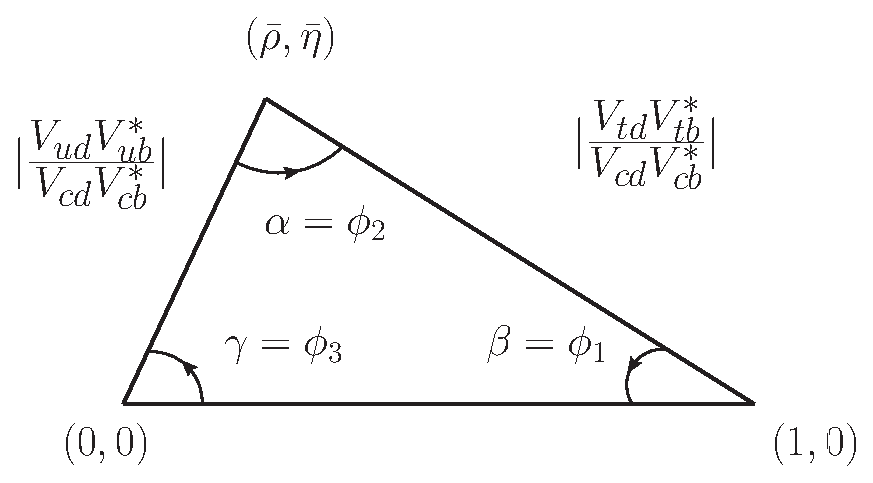
\includegraphics[width=0.5\textwidth]{theory/unitarity.eps}
\caption{Unitarity triangle in a complex plane.}
\label{fig:unitr}
\end{figure}
The area of the triangle is half of the Jarlskog invariant \textit{J}, a quantifier of CP violation, which is defined as $\rm{Im}[V_{ij}V_{kl}V^*_{il}V^*_{kj}]$ \cite{Jarlskog:1985ht}. It is interesting to notice that the \gls{SM} with its parameters may or may not violate CP. Only after measuring \textit{J} it is possible to determine the CP non-conservation. \textit{J} vanishes only if the mixing angle $\theta_{ij} = \{0 , \pi/2\}$; $\delta = \{0 , \pi\}$. So measurements of \textit{J} allows to verify that the \gls{CKM} matrix is complex and hence different mixing for quarks and anti-quarks is obtained.% although \gls{SM} CP violation is not big enough to explain the matter dominated universe.

The \gls{CKM} matrix elements which comprise of magnitudes and phases can be determined in different ways but the most precise option employs a global fit to all available measurements as shown in~\autoref{fig:unifit}. Hence, the most precise measurement of the \gls{CKM} matrix magnitudes to-date \cite{Patrignani:2016xqp} is 
%\begin{equation}|V_{\rm CKM}| = \begin{pmatrix}0.97446 \pm 0.00010 & 0.22452 \pm 0.00044  & \colorboxed{green}{0.00365\pm 0.00012} \cr
%	0.22438 \pm 0.00044 &  0.97359 \bfrac{+0.00010}{-0.00011} & 0.04214\pm 0.00076 \cr
%0.00896 \bfrac{+0.00024}{-0.00023} & 0.04133 \pm 0.00074 &  0.999105 \pm 0.000032 \cr \end{pmatrix},
%\end{equation}
\begin{equation}|V_{\rm CKM}| = \begin{pmatrix} 0.97434\bfrac{+0.00011}{-0.00012} & 0.22506 \pm 0.00050 & \colorboxed{green}{0.00357 \pm 0.00015}\cr
	0.22492 \pm 0.00050 &  0.97351 \pm 0.00013 & 0.0411 \pm 0.0013 \cr
0.00875 \bfrac{0.00032}{-0.00033} &  0.0403 \pm 0.0013 & 0.99915 \pm 0.00005  \cr \end{pmatrix},
\end{equation}
with non-zero Jarlskog invariant $J=(3.18\pm0.15)\times 10^{-5}$. Highlighted is the result for magnitude of the $V_{ub}$ matrix element, $|V_{ub}|$, which is the element with highest fractional uncertainty on its value. Therefore precise measurement of this element is very important and was the original motivation for the analysis of \Bmumumu. Moreover, as displayed in~\autoref{fig:unifit}(a)(b), the measurement of $|V_{ub}|$ (orange circle)(green circle) together with $\sin(2\beta)$ measurement (green band)(blue band) constrain the apex of the triangle. This means that these two measurements together with other measurements test the unitarity of the \gls{CKM} matrix, one of the fundamental assumptions of the \gls{SM}.


\begin{figure}[h]
\centering
%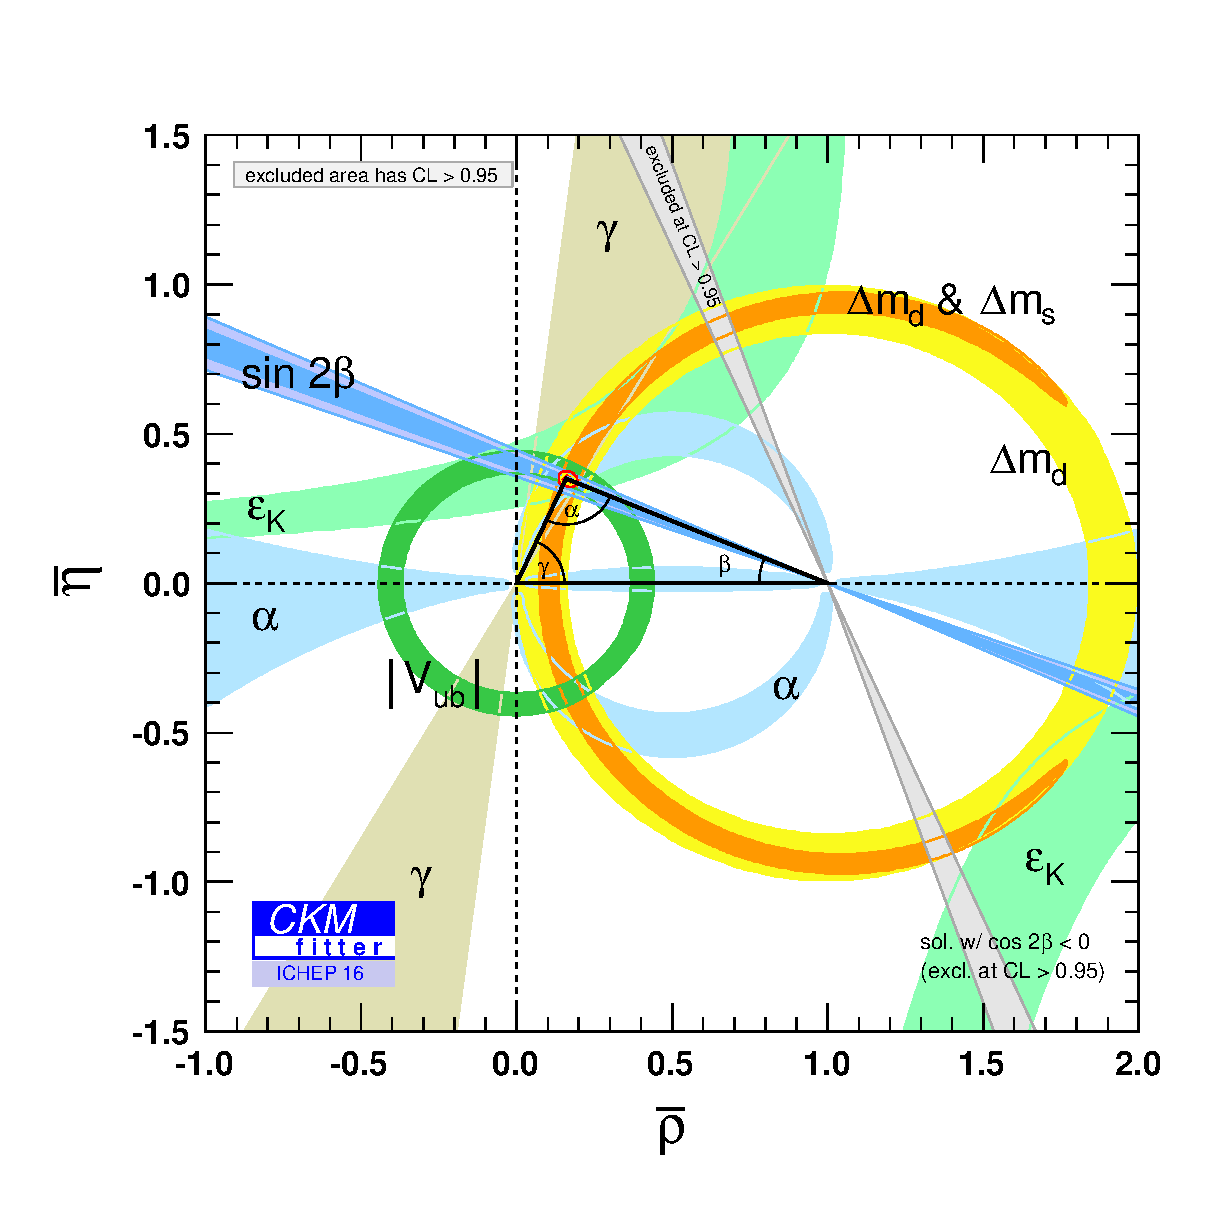
\includegraphics[width=0.7\textwidth]{theory/rhoeta_large_lol.eps}
\vspace*{-1.5cm}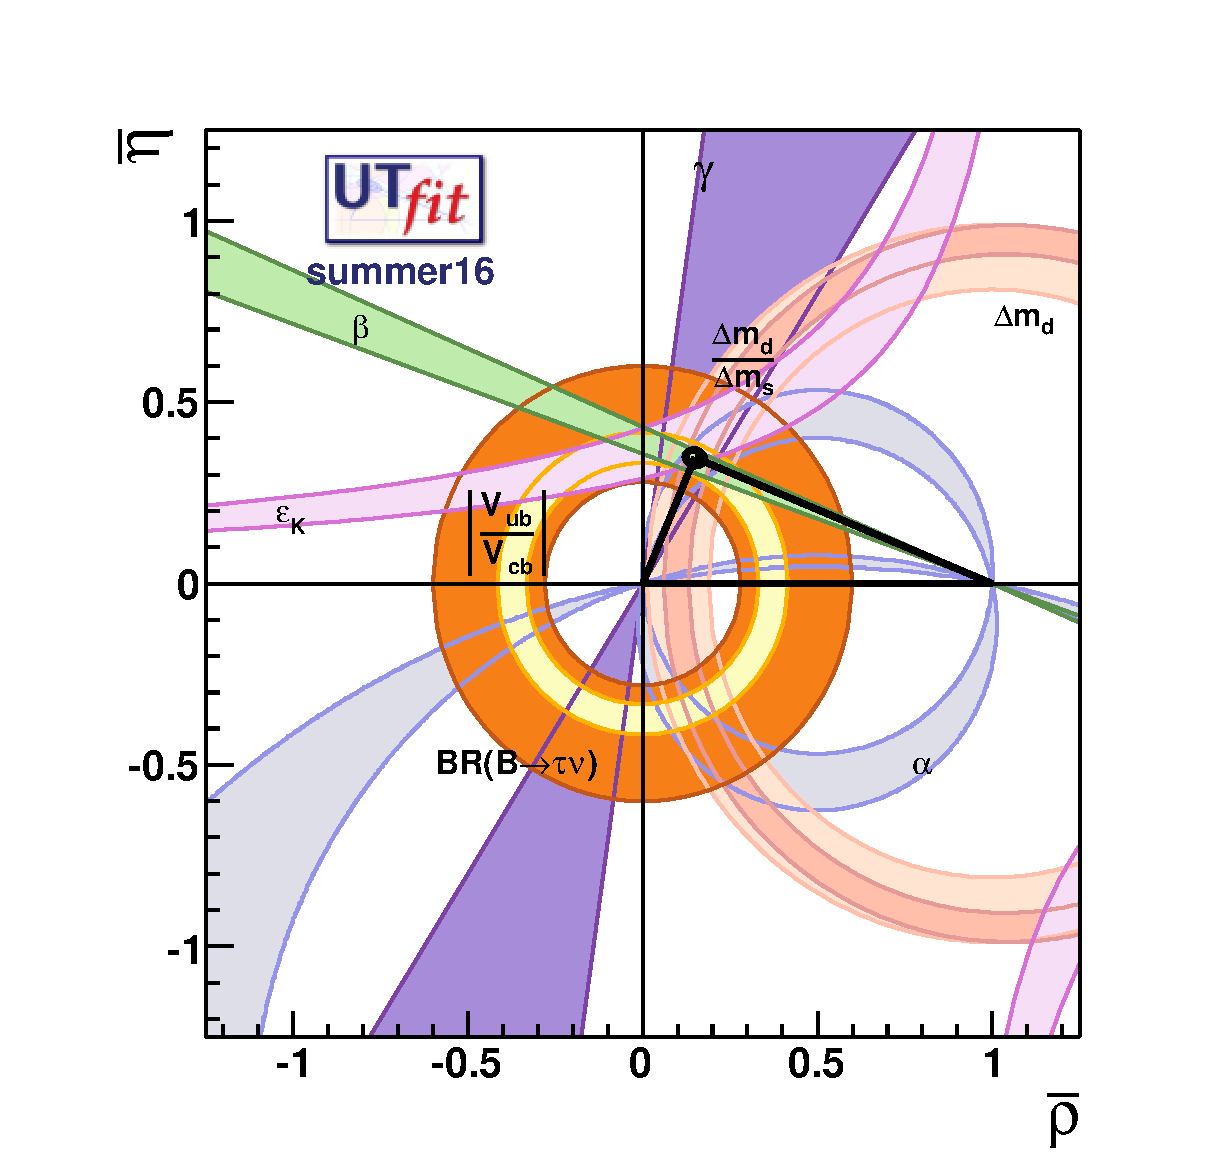
\includegraphics[width=0.65\textwidth]{theory/rhoeta-fullfit-sm.eps}\put(30,130){(a)}
\newline
\hspace*{-1.7cm}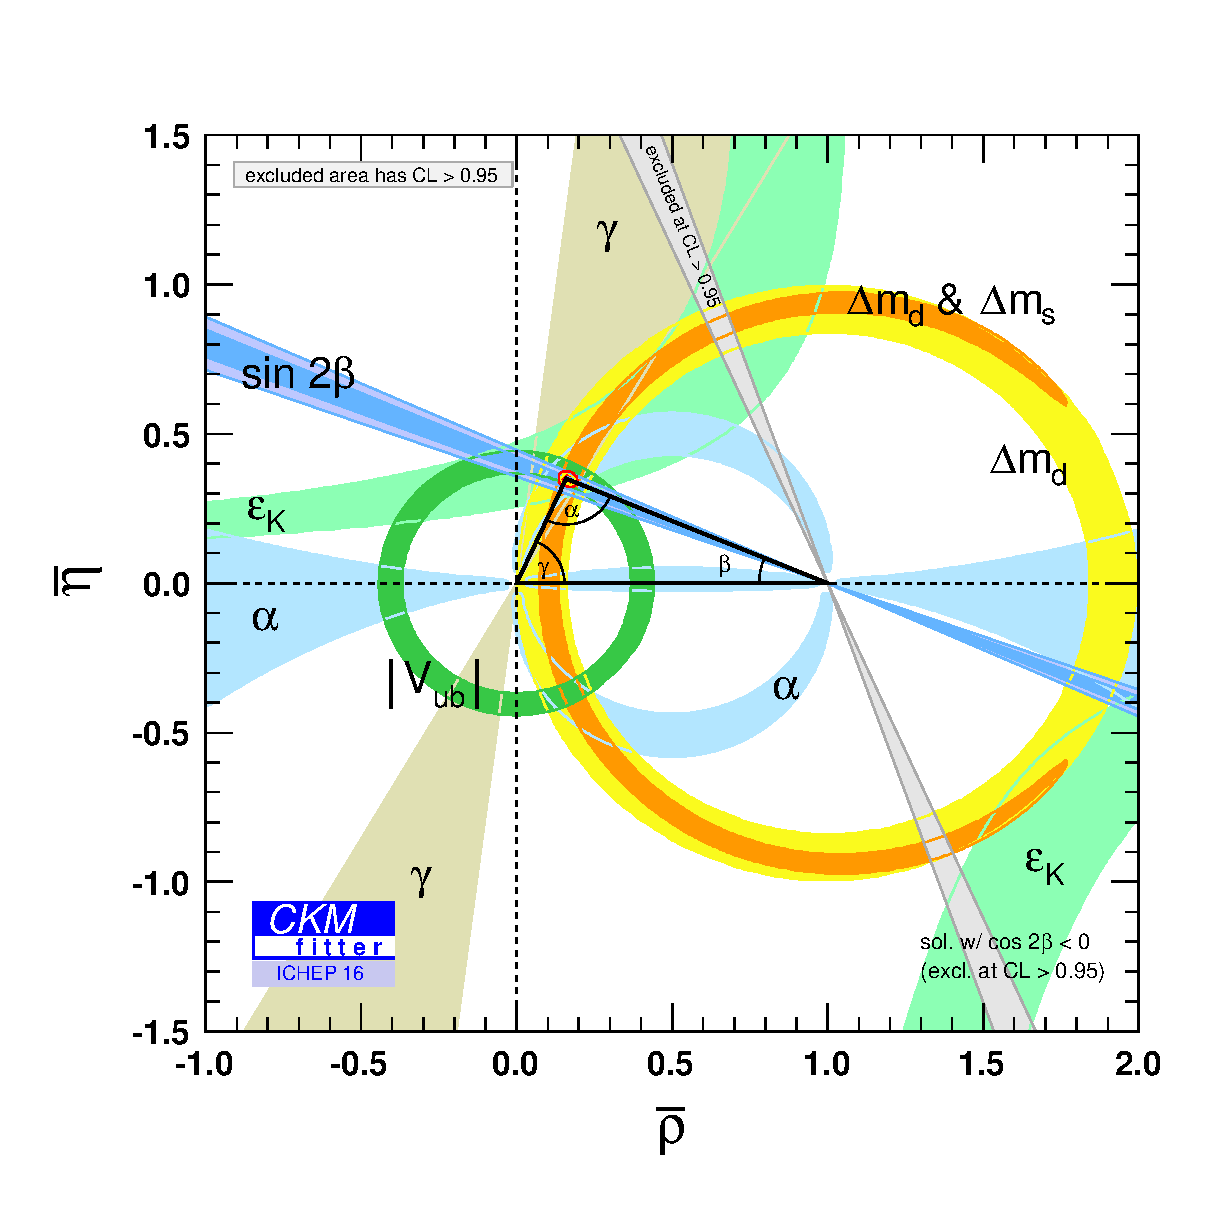
\includegraphics[width=0.65\textwidth]{theory/rhoeta_large_lol.eps}\put(30,130){(b)}
\caption{Different experimental measurements that constrain the \gls{CKM} matrix elements together with the global fit results from two collaborations (a) UTFit and (b) CKMFitter as of summer 2016. This figures are taken from \cite{Bona:2006ah} and \cite{Charles:2004jd}. There is a good agreement for the results between the two different collaborations.}
\label{fig:unifit}
\end{figure}


\section{Fully Leptonic \mb{P^{+}\rightarrow l^{+} \nu} Decays}
\label{lnudecays}
%This text is based on a summary provided by PDG on Leptonic Decays of Charged Pseudoscalar Mesons.
Purely leptonic decays that proceed via annihilation-type diagrams of pseudoscalar mesons ($P$) are of great interest for flavour physicists because they allow to make:
\begin{itemize}
\item either measurements of the \gls{CKM} matrix elements,
\item or measurements of leptonic decay constants,
\item or measurements of new physics effects.
\end{itemize}
The first two types of measurements are possible because the decay rates of $P^{+}\rightarrow l^{+} \nu$ decays are sensitive to the product of the appropriate \gls{CKM} matrix element ($V_{q_{1}q_{2}}$ where $q_{1}$ and $q_{2}$ are constituent quarks of the pseudoscalar meson) and decay constant $f_{P}$, related parameter arising from the strong interaction. In more detail, the decay width of a fully leptonic decay of a pseudoscalar meson in the \gls{SM} to the lowest order can expressed as 

\begin{equation}
%\label{eqn:br} 
\Gamma(P^{+} \rightarrow {l^{+}} \nu)=  
	\frac{G_{F}^{2} m^{}_{P^{+}}  m_{l^{+}}^{2}}{8\pi} 
	\left[1 - \frac{m_{l^{+}}^{2}}{m_{P^{+}}^{2}}\right]^{2}  
	f_{P}^{2} |V_{q_{1}q_{2}}|^{2} 
	,
\label{eqn:dw} 
\end{equation}
where
$G_F$ is the Fermi constant,
$m^{}_{P^{+}}$ and $m_{l^{+}}$ are the pseudoscalar meson and lepton masses, respectively. This decay width can be compared to that of $\tau \rightarrow l\nu \bar{\nu}$\cite{Marciano:1988vm}


\begin{equation}
%\label{eqn:br} 
\Gamma(\tau \rightarrow {l} \nu \bar{\nu})=
	\frac{G^{2}_{l\tau} m^{5}_{\tau}}{192\pi^{3}}\left[1-f\big(\frac{m^{2}_{l'}}{{m^{2}_{\tau}}}\big)\right],
\label{eqn:tauonic} 
\end{equation}
where $G_{l\tau}$, is relevant Fermi constant. In this case $ f(x) = 1  8x - 8x^{3} + x^{4} + 12x^{2}\mathrm{log}(x)$ represents a correction due to the mass of the lepton
%(finite lepton mass)
in the final state. Corrections arising from the $W$ propagator effects are negligible for this decay and are not considered here and nor are radiative corrections so that only the lowest order contributions are considered. As compared to~\autoref{eqn:dw} the decay width is significantly higher. 

So in order to measure the \gls{CKM} matrix amplitude, knowledge of $f_{P}$ must be inferred. $f_{P}$ can be calculated using lattice \gls{QCD} techniques and together with experimental determination of the decay rates provide a way to determine the amplitude squared of the relevant \gls{CKM} matrix element assuming there is no contribution from new physics. More conventionally, \gls{CKM} magnitudes are determined from semileptonic decays, which is experimentally 
more accessible but entails larger theoretical uncertainty.
%\gls{CKM} magnitudes are determined from semileptonic decays different type of current is given \mybox{this is in pdg i dont understand why is it wrong}. In purely leptonic decays axial-vector flavour-changing currents ($q_{1}\gamma_{\mu}\gamma_{5}q_{2}$) are probed as opposed to vector current ($q_{1}\gamma_{\mu}q_{2}$) in semileptonic case.

Vice versa, assuming unitarity of \gls{CKM} triangle and experimental determination of relevant $V_{q_{1}q_{2}}$ one can obtain experimental determination of the decay constants and compare it with theoretical prediction.

Last, but not least, is of course the measurement of presence of new physics in these decays. Especially appealing is the presence of new particles which would manifest themselves in the decay rates of heavier pseudoscalars ($D_{(s)}$ or $B$). An example of such new particles include charged Higgs bosons, $H^{\pm}$, coming from so-called Type II Higgs-doublet models \cite{Hou:1992sy}\cite{Akeroyd:2003zr}\cite{Dobrescu:2008er} or leptoquarks\cite{Dobrescu:2008er}. In this case, considering $B^{+}\rightarrow l^{+}\nu$ decay, the four-fermion interaction between $W^{\pm}$ and $H^{\pm}$ would modify the \gls{SM} decay width~\autoref{eqn:dw} to
%remember branching fraction is partial width of total width
%total width  h over liftime so lifetime is always missing from equations 
% see https://www2.ph.ed.ac.uk/~vjm/Lectures/ParticlePhysics2010_files/Particle3-2Nov.pdf this

\begin{equation}
\Gamma(B^{+} \rightarrow {l^{+}} \nu)=  
        \frac{G_{F}^{2} m^{}_{B^{+}}  m_{l^{+}}^{2}}{8\pi} 
        \left[1 - \frac{m_{l^{+}}^{2}}{m_{B^{+}}^{2}}\right]^{2}  
	f_{P}^{2} |V_{ub}|^{2} \,\times\, r_H,
%\Gamma(B^+\to \ell^+\nu_\ell)={G_F^2 m_{B} m_l^2 f_{B}^2\over 8\pi}
%|V_{ub}|^2 \left(1-{m_l^2\over m^2_{B}}\right)^2 \,\times\, r_H
\end{equation}
where
\begin{equation}
	r_H=[1-\tan^2\beta(m^{2}_{B^{+}}/m^{2}_{H^{+}})]^2.
\end{equation}
Here $\tan\beta = \frac{v_{2}}{v_{1}}$, where $v_{i}$ are the vacuum expectation values for the Higgs doublets. In order to have an enhancing effect for the rate of the $B^{+}\rightarrow l^{+}\nu$ decay (to have $r_{H}>1$), $\tan\beta/m_{H^{\pm}}> 0.27 \gev^{-1}$. The experimental limit presents already a strong lower bound on the charged Higgs mass $m_{H^{\pm}}>600\gev$\cite{Arbey:2017gmh}. This makes the most of the parameter space in $\tan\beta$ and $m_{H^{\pm}}$ satisfy enhancing condition of $\tan\beta/m_{H^{\pm}}>0.27 \gev^{-1}$.

The ratio of rates between $P\rightarrow\tau\nu$, $P\rightarrow\mu\nu$ and $P\rightarrow e\nu$ decays could also be of an interest. In the ratios the decay constant $f_{P}$ cancels out making such measurements a good tool for lepton universality tests.

As seen in~\autoref{eqn:dw}, a purely leptonic final state going through $P\rightarrow W^{*}\rightarrow l \nu$ is suppressed by $\frac{m^{2}_{l}}{m^{2}_{p}}$, also known as helicity suppression. This suppression occurs as a result of angular momentum conservation. In case of $B^{+}\rightarrow l^{+} \nu$, the $B^{+}$ is a spin-0 particle and hence its decay products should have spin 0 combined, or in other words, be anti-aligned. Neutrinos in the \gls{SM} are always produced left-handed. As the spin of the antilepton and the neutrino should be anti-aligned, the antilepton also needs to be left-handed (to have negative helicity). However, the weak current only couples to right-handed antiparticles. Therefore, the antilepton has to be boosted in order to have different helicity. For massless particles such a helicity flip is not possible making this decay impossible. The lighter the lepton, the larger the velocity and hence higher boost is necessary, making decays to lighter leptons rarer even though they have bigger kinematic phase space available.

%https://www.physicsforums.com/threads/helicity-and-suppression.804600/
Concentrating on the decays $B^{\pm}$ meson, the latest experimental measurements for rates of $B^{+}\rightarrow l^{+} \nu$ decays have been performed by $B$ factories, finding evidence for $B^{+}\rightarrow \tau^{+}\nu$ and first sign of $B^{+}\rightarrow \mu^{+}\nu$ as seen in~\autoref{tab:sum}. These results are to be compared with the \gls{SM} predictions $\mathcal{B}(B^{+}\rightarrow \tau^{+}\nu) = (0.82+0.03-0.02)\times10^{-4}$\cite{Charles:2004jd} and $\mathcal{B}(B^{+}\rightarrow \mu^{+}\nu) = (3.80\pm0.31)\times10^{-7}$\cite{Sibidanov:2017vph}, which are obtained by using $|V_{ub}|$ value resulting from other measurements and lattice calculations of $f_{B}$. %Quite substantial statistical as well as systematical errors show the difficulty of this type of measurements. 



\begin{table}[ht]
\begin{center}
\begin{tabular}{ l l l l H c H} \toprule
        Process &Experiment & Tag &${\mathcal{B}}$ & Published & Significance & {$|V_{ub}|f_{B^+}$ (MeV)} \hfill\\
	 & &  & & & [$\sigma$] & {$|V_{ub}|f_{B^+}$ (MeV)} \hfill\\
\hline\\[-2.5ex]
        $B^{+}\rightarrow \tau^{+}\nu$  &Belle~\cite{Adachi:2012mm}&Hadronic&$(0.72^{+0.27}_{-0.25}\pm0.11)\times10^{-4}$  & 2013 & 3.0 \\
        $B^{+}\rightarrow \tau^{+}\nu$  &Belle~\cite{Kronenbitter:2015kls}&Semileptonic&$(1.25\pm0.28\pm0.27)\times10^{-4}$ & 2015 & 3.8 \\
        $B^{+}\rightarrow \tau^{+}\nu$  &Belle~\cite{Kronenbitter:2015kls}&Average&$(0.91 \pm 0.22)\times10^{-4}$ & 2015 & 4.6 \\\hline\\[-2.5ex]
        $B^{+}\rightarrow \tau^{+}\nu$  &BaBar~\cite{Lees:2012ju} & Hadronic & $(1.83\,^{+0.53}_{-0.49}\pm0.24)\times10^{-4}$ & 2012 & 3.8 \\
        $B^{+}\rightarrow \tau^{+}\nu$  &BaBar~\cite{Aubert:2009wt} & Semileptonic & $(1.7\pm 0.8\pm 0.2)\times10^{-4}$ & 2010 & 2.3\\
        $B^{+}\rightarrow \tau^{+}\nu$  &BaBar~\cite{Lees:2012ju} & Average & $(1.79 \pm 0.48)\times 10^{-4}$ & 2012 & - & $1.01\pm 0.14$  \\ \hline
$B^{+}\rightarrow \mu^{+}\nu$ & Belle~\cite{Sibidanov:2017vph} & Untagged& $(6.46\pm2.22\pm 1.60)\times 10^{-7}$ & 2017 & 2.4 &\\
%        & Our average & &$1.06\pm0.20$&$0.77\pm0.07$ & & \\
\bottomrule
\end{tabular}
\end{center}
\caption{Experimental summary of searches for $B^{+}\rightarrow l^{+}\nu$ that is inspired from \cite{Patrignani:2016xqp}. Tag Hadronic/Semileptonic/Untagged refers to different way data is selected in Belle and BaBar factories.}
\label{tab:sum}
\end{table}




With helicity suppressed rates and very limited signatures in the detector (one charged track for muons and electron, more charged tracks for taus, but also more missing energy depending on the reconstruction channel) searching for such decays is very challenging. In order to make measurements of the same kind (CKM precision measurements, decay constants measurements, new physics searches), fully leptonic decays with photons can be considered.   

\section{Fully Leptonic \mb{B^{+}\rightarrow l^{+} \nu \gamma} Decays}
\label{lnugamma}
The helicity suppression of $B^{+}\rightarrow l^{+} \nu$ decays can be lifted by considering the decay with an additional photon radiated from the $B^{+}$ meson, at the cost of the electromagnetic suppression with coupling constant $\alpha_{em}$. Consequently, the branching fraction for radiative decays can be comparable or even larger than the corresponding fraction for purely leptonic decays. It has been shown that $R^{\mu}_{B}=\frac{\Gamma(B\rightarrow \mu \nu \gamma)}{\Gamma(B\rightarrow \mu \nu)}\approx(1-20)$ making $\mathcal{B}(B\rightarrow \mu \nu \gamma)\approx(10^{-7}-10^{-6})$ \cite{Burdman:1994ip}.

%As compared to photonless decays, the amplitude of the decay will have a contribution from both the axial-vector weak current as well as the vector current.
The differential decay width with $\frac{1}{m_{b}}$ and radiative corrections
at next-to-leading logarithmic order calculated in\cite{Beneke:2011nf} is given by
\begin{equation}
\frac{d\Gamma}{dE_{\gamma}} = \frac{\alpha_{em}G^{2}_{F}|V_{ub}|^{2}}{48 \pi^{2}}m_{B}^{4}(1 - x_{\gamma})x_{\gamma}^{3}[F_A^{2} + F_V^{2}],
\end{equation}
 where $x_{\gamma} = 2E_{\gamma}/m_{B}$, $F_A$ is the axial form factor and $F_V$  is the vector form factor defined as
\begin{equation}
F_{V}(E_{\gamma}) = \frac{Q_{u}m_{B}f_{B}}{2E_{\gamma}\lambda_{B}(\mu)} R(E_{\gamma}, \mu) + [\xi(E_\gamma) +  \frac{Q_{u}m_{B}f_{B}}{(2E_{\gamma})^{2}} + \frac{Q_{b}m_{B}f_{B}}{2E_{\gamma}m_{b}}],
\label{eq:top1}
\end{equation}

\begin{equation}
F_{A}(E_{\gamma}) = \frac{Q_{u}m_{B}f_{B}}{2E_{\gamma}\lambda_{B}(\mu)} R(E_{\gamma}, \mu) + [\xi(E_\gamma) -  \frac{Q_{u}m_{B}f_{B}}{(2E_{\gamma})^{2}} - \frac{Q_{b}m_{B}f_{B}}{2E_{\gamma}m_{b}} + \frac{Q_{l}f_{B}}{E_{\gamma}}].
\label{eq:top2}
\end{equation}
Here $Q_{l},Q_{u},Q_{b}$ are the charges of the lepton, up quark, and
bottom quark, respectively, and $R(E_{\gamma}, \mu)$ is a radiative correction
calculated at the energy scale $\mu$ %that equals one at tree level.
and $m_{b}$ is the mass of the $b$ quark.

The first term in~\autoref{eq:top1} and ~\autoref{eq:top2} represents the leading-power contribution in the heavy-quark expansion. Note that this term
is the same for the vector and axial form factor. The second terms are $\frac{1}{m_{b}}$ power corrections relative to the leading term. Further corrections have been discussed in~\cite{Wang:2016beq}.



Recent measurement of the radiative $B^{+} \rightarrow l^{+} \nu \gamma$, where $l^{+}$ is either $e^{+}$ or $\mu^{+}$ was performed by Belle using hadronic tagging on their full data sample\cite{Heller:2015vvm}. The search yielded $\mathcal{B}(B^{+}\rightarrow \mu^{+} \nu \gamma) < 3.4\times 10^{-6}$ and $\mathcal{B}(B^{+}\rightarrow e^{+} \nu \gamma) < 6.1\times 10^{-6}$.



\section{Fully Leptonic \mb{B^{+}\rightarrow l^{+} l^{-} l^{+} \nu} Decays}
\label{mydecay}

In LHCb, the most optimal approach due to the detector capabilities is to measure this kind of decay by converting the photon into a pair of muons, see~\autoref{fig:myfeyn}(a). If the naive expectation of only taking into account photon conversion into two muons is adopted, then the expected branching fraction for this analysis is $\mathcal{B}(B^{+}\rightarrow \mu^{+} \mu^{-} \mu^{+} \nu) \approx 1.0\times 10^{-8}$. However, such estimate is not correct because there are other contributions to the total decay rate as shown in the first theoretical prediction for $\mathcal{B}(B^{+}\rightarrow \mu^{+} \mu^{-} \mu^{+} \nu)$ in \cite{Danilina:2018uzr} based on the Vector Meson Dominance (VMD) model. This theoretical prediction yields $\mathcal{B}(B^{+} \rightarrow \mu^{+} \mu^{-} \mu^{+} \nu) \approx 1.3\times 10^{-7}$.% and the rest of this section is a short summary of this publication.

 The VMD model was formulated to describe the interaction between photons and hadrons before \gls{QCD} was formulated. It is an approximative model where the photon is treated to be made of a purely electromagnetic component and a vector meson component. This idea originates in the fact that both photon and vector mesons have the same quantum numbers $J^{PC} = 1^{-\ -}$ and if two particles have the same quantum numbers then they mix. %(the state which commutes with the Hamiltonian is a superposition of all such states). 
% Therefore, there is mixing between photons and vector mesons.

As mentioned previously, there are different contributions to the amplitude of the $\mathcal{B}(B^{+}\rightarrow \mu^{+} \mu^{-} \mu^{+} \nu)$. Using the VMD model, it is not surprising that the biggest contribution arises from the photon emission from the valence $u$-quark of the $B$ meson. In this case, the contribution from the $\rho(770)$ and $\omega(782)$ resonances are included in the calculation. Secondly, the contribution of photon emission from the $b$-quark is studied, effectively creating excited $B^{+}$, $B^{+*}$ intermediate resonance state. Thirdly, the photon can be emitted from the final-state lepton, a process known as Bremsstrahlung. All these different contributions to the decay amplitude are shown in~\autoref{fig:myfeyn}. To obtain the total amplitude, the sum of the matrix elements of the three contributions is calculated in the limit where $m_{l}$ is set to zero.


\begin{figure}[ht]
\centering
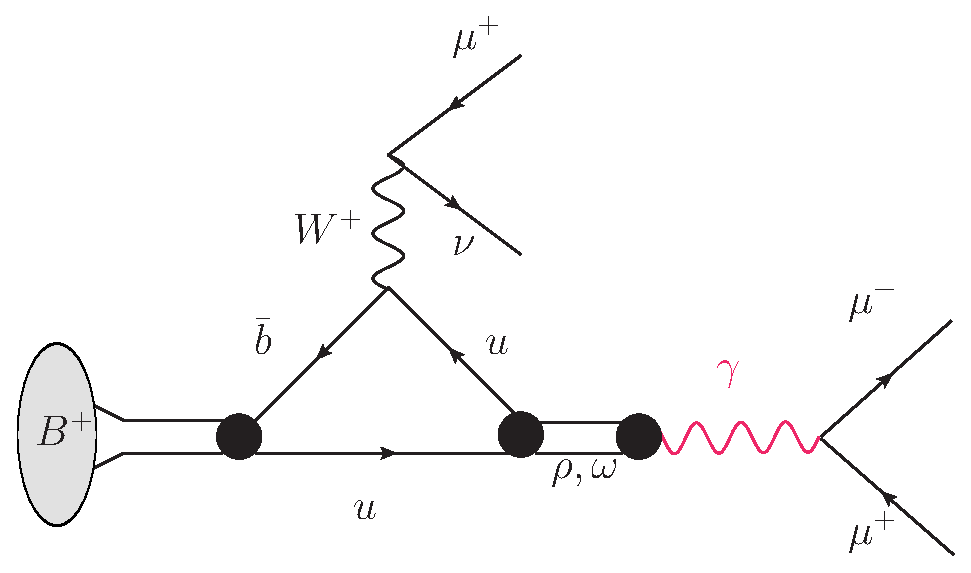
\includegraphics[scale=0.5]{theory/nik_1figure}\put(-30,133){(a)}
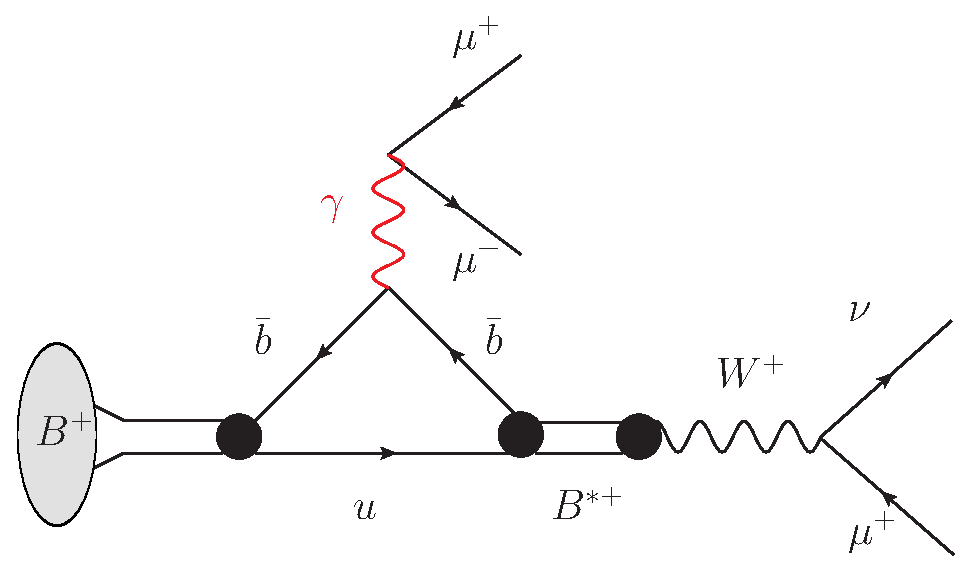
\includegraphics[scale=0.5]{theory/nik_2figure}\put(-30,133){(b)}
\newline
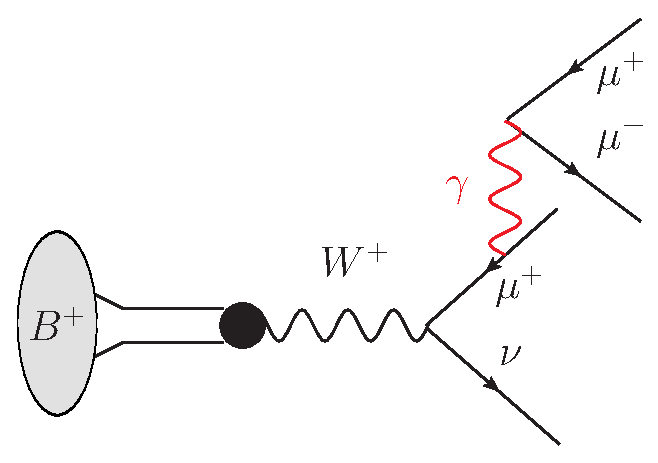
\includegraphics[scale=0.55]{theory/nik_3figure}\put(-30,133){(c)}
\centering
	\caption{Different contributions to the \Bmumumu decay. (a) Initial $u$-quark state radiates off a virtual photon which decays into a pair of muons and the $W^{+}$ decays into a muon and muon neutrino. Most of the contribution to the rate comes from hadronic contribution to the photon. (b) Photon emission from $b$-quark and (c) finally emission from the final state muon.}
\label{fig:myfeyn}
\end{figure}


In this publication the amplitude of $\mathcal{B}(B^{+}\rightarrow \mu^{+} \mu^{-} \mu^{+} \nu)$ is estimated by calculating $\mathcal{B}(B^{+}\rightarrow \mu^{+} \mu^{-} e^{+} \nu)$ amplitude first and then adding a negative interference term that arises due to the identical fermions in the final state doubling the number of possible diagrams. The numerical calculation yields $\mathcal{B}(B^{+}\rightarrow \mu^{+} \mu^{-} e^{+} \nu) \approx 1.3 \times 10^{-7}$ and $\mathcal{B}(B^{+}\rightarrow \mu^{+} \mu^{-} \mu^{+} \nu) \approx 1.3 \times 10^{-7}$. 

\section{The \mb{\Bmumumu} Decay Model}
\label{simulation}
As the search for the \Bmumumu decay is the first of its kind, a simulation that describes this type of decay was not available. There are, however, three types of decay models for \Bmumumu which were adopted and used for different purpose. More detail about their use is covered in~\autoref{SimulationSamples}.

For any decay, it is possible to use a phase space model, \textit{PHSP}, which only takes into account the kinematic constraints of the decay without taking into account any input from theoretical considerations as the matrix element is constant. This is not satisfactory for decays where there are intermediate virtual photons or vector meson resonances.

The following decay model is developed to reflect the expected behaviour of decays shown in~\autoref{fig:myfeyn}. The decay proceeds through a virtual $W$ decaying to $\mu^{+} \nu$ and a virtual photon decaying to a muon pair. This has similar structure to $\B^{+} \rightarrow (K^{*+}) \mu^{+} \mu^{-}$ decay, where the $K^{*+}$ can take the role of the virtual $W$ decay. By using the \textit{BTOSLLBALL} model\cite{Ali:1999mm}, traditionally used for $B^{+} \rightarrow (K^{*+}) l^{+} l^{-}$ decays, but modifying the properties of the $K^{*+}$ to those of virtual $W$ (having mass of 0.1 \gevcc and width 50 \gev), it is possible to obtain a good approximation to the correct features of the decay. This is visible in~\autoref{fig:mcgeneration}, where there is a characteristic photon pole for low $q(\mu^{+},\mu^{-})$, invariant mass of the opposite muon pair, and flat distribution for $K^{*}(\mu^{+}, \nu) $, invariant mass of the muon and neutrino pair. This decay model will be further referred to as \textit{INSP} model. 



%\mybox{Sally: move it to theory and check ulrik's comment} In order to produce simulation with a decay model which is more representative of the spin structure involved, the following strategy is adapted. In this simulation approach, the decay proceeds as follows: \Bpm decays into \Wpm and a pair of opposite sign muons and then \Wp is decayed to $\mu^{+} \nu$. \textit{BTOSLLBALL} model\cite{Ali:1999mm}, traditionally used for $\B \rightarrow (K,K^{*}) l^{+} l^{-}$ decay, with the form factor calculations can be used to simulate $\Bpm \rightarrow \Wpm l^{+} l^{-}$ decay. After that, \Wp is decayed to $\mu^{+} \nu$ using \textit{PHSP}. For semileptonic $b \rightarrow s l^{+} l^{-}$ transitions, there is a characteristic photon pole for low $q(\mu^{+},\mu^{-})$, invariant mass of the opposite muon pair, and flat distribution for $K^{*}(\mu^{+}, \nu) $, invariant mass of the muon and neutrino pair. In order to achieve this, a new pseudo-particle is introduced to EVTGEN with specific properties, $K^{*}(\mu^{+}, \nu)$, and the best output can be seen to be for a particle $K^{*}(\mu^{+}, \nu)$ with mass to be set to $0.1 \text{GeV/c}^{2}$, and width, corresponding to $\tau= 1.3\times10^{-17}$ nanoseconds as can be seen in~\autoref{fig:mcgeneration}. This procedure was also applied for the charge conjugate case. This model is denoted as \textit{INSP} and is used as default in mass fits and efficiency calculations.

\begin{figure}[h!]
\centering
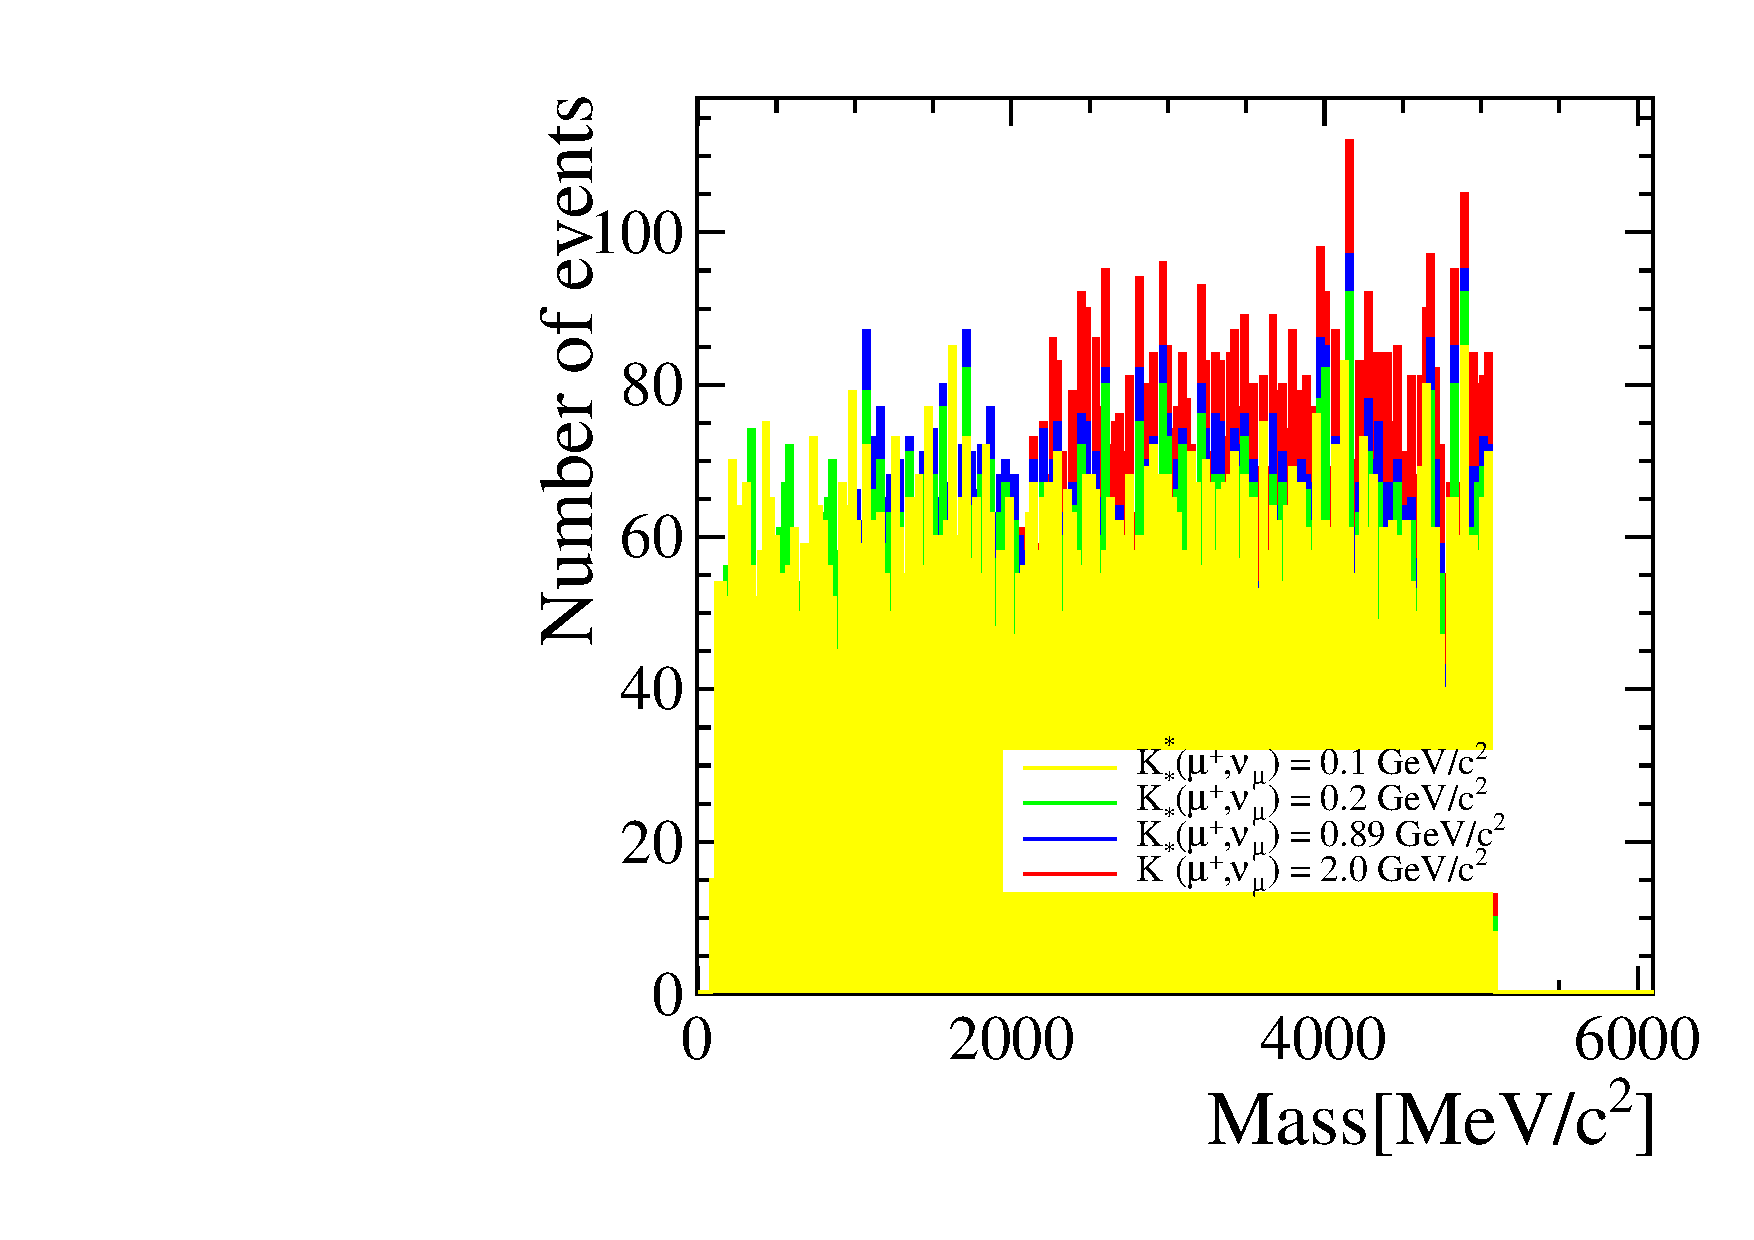
\includegraphics[width=0.5\linewidth]{./sel/reporttry_new}\put(-70,133){(a)}
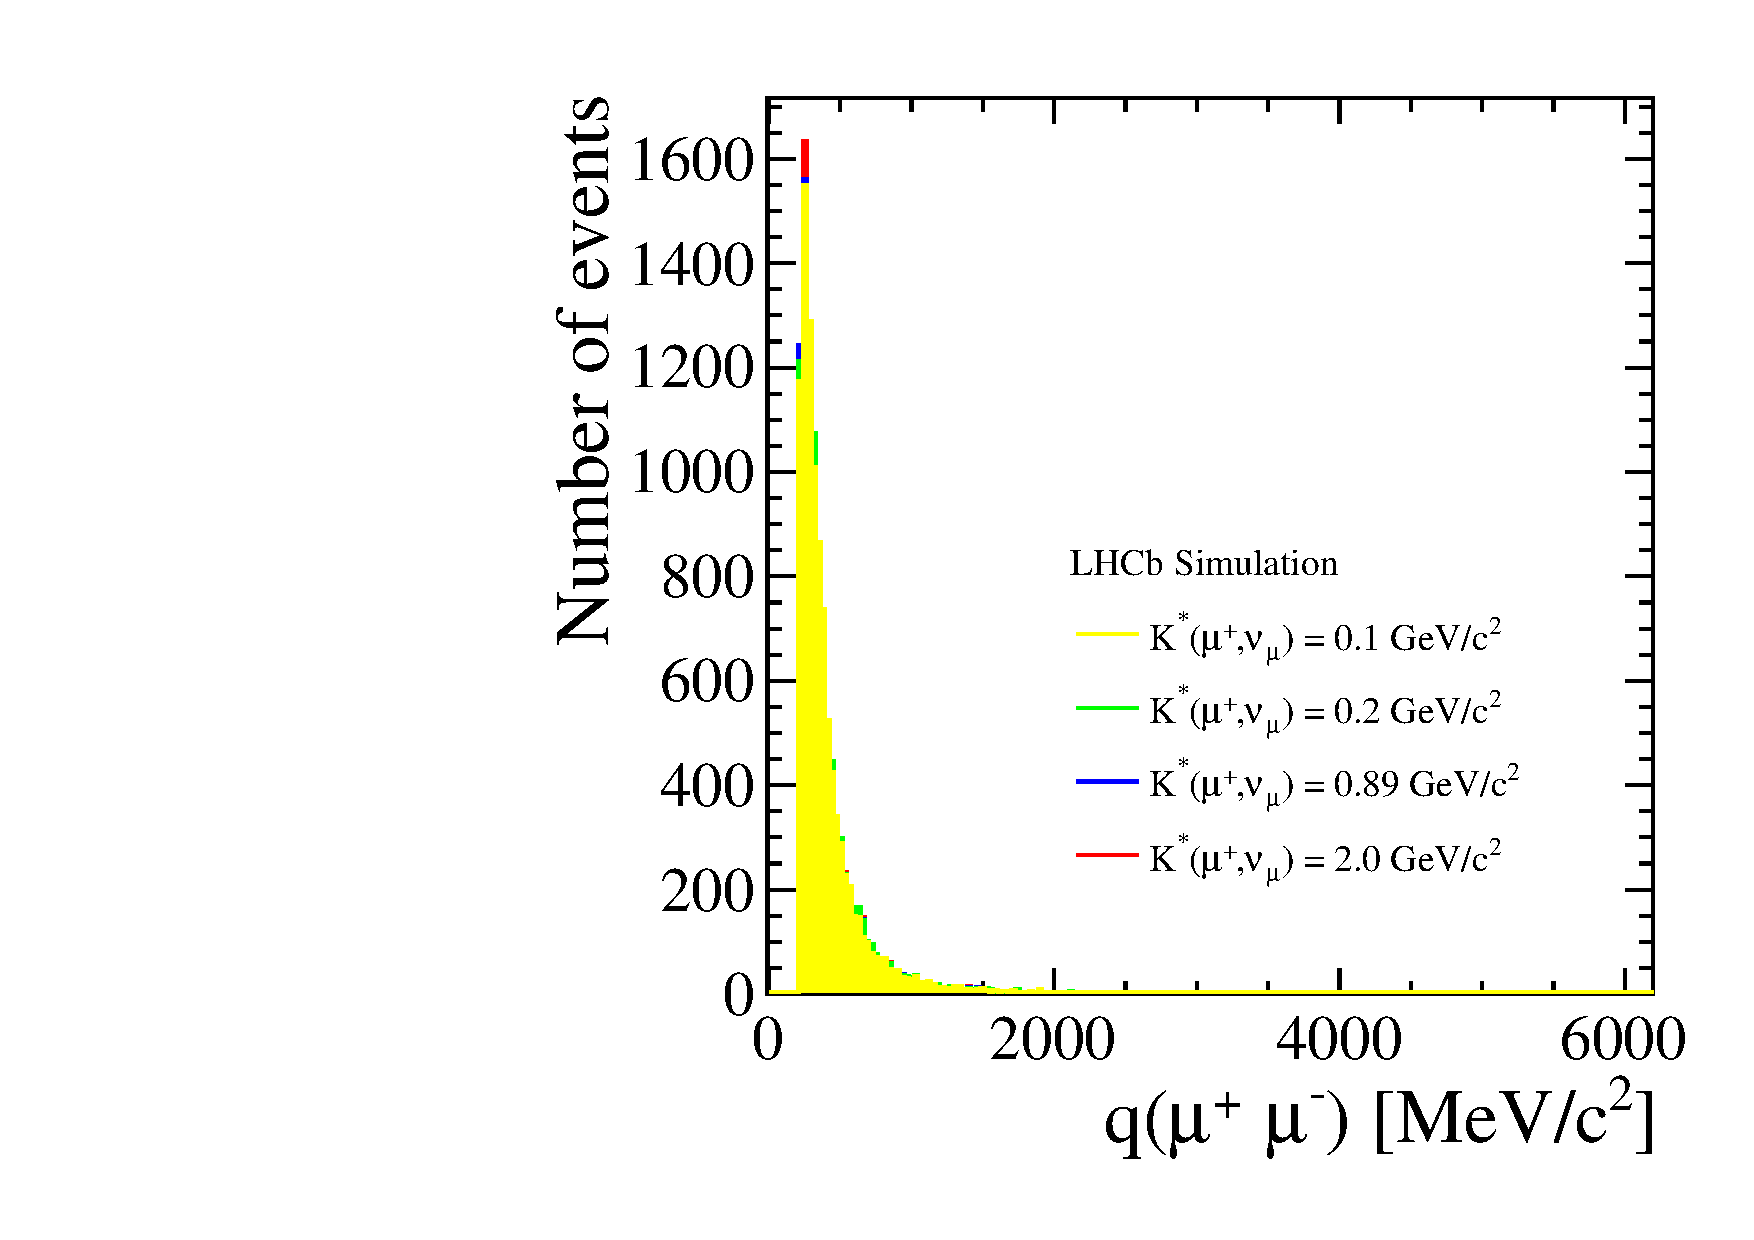
\includegraphics[width=0.5\linewidth]{./sel/reporttrialqpres_new}\put(-50,133){(b)}
\caption{Distributions for signal simulation. (a) $K^{*}(\mu^{+}, \nu)$ (b) $q(\mu^{+},\mu^{-})$ distributions under different $K^{*}$ mass hypotheses. The most flat distribution in $K^{*}(\mu^{+}, \nu)$ is plotted in yellow.}
\label{fig:mcgeneration}
%\vspace*{-1.0cm}
\end{figure}

Finally, there is a decay model based on calculations from VMD model, which was written by authors of \cite{Danilina:2018uzr}. This model denoted as \textit{NIKI}.

\chapter{The LHCb Detector}
\label{chap:dec}

\textit{In this section, an overview of the accelerator complex at CERN as well as the physics motivation behind the \Gls{LHCb} detector and its design will be described.}

CERN has built one of the most exciting laboratories to study elementary particle interactions in the world. Its complex set of particle accelerators and detectors is shown in~\autoref{fig:AcceleratorComplex}. The process of accelerating protons starts with the source of protons. Protons are obtained from a hydrogen gas bottle by applying an electric field separating hydrogen into protons and electrons. The first proton accelerator in the chain, Linac 2, accelerates the protons to the energy of 50 \mev. Linac 2 is a tank composed of several chambers where the resonant cavities are tuned to a specific frequency creating potential differences in them, which then make the protons accelerate. The protons are then injected into the Proton Synchrotron Booster (\Gls{PSB}), where they are accelerated further to 1.4 \gev. The next in line is the Proton Synchrotron (\Gls{PS}) reaching energy of 25 \gev. Before either entering the Large Hadron Collider (\Gls{LHC}) or North Area (mainly used as testing facility for experiment upgrades) the Super Proton Synchrotron (\Gls{SPS}) is the last accelerator in the chain. Here proton acceleration to 450 \gev is achieved.

\begin{figure}
  \centering
  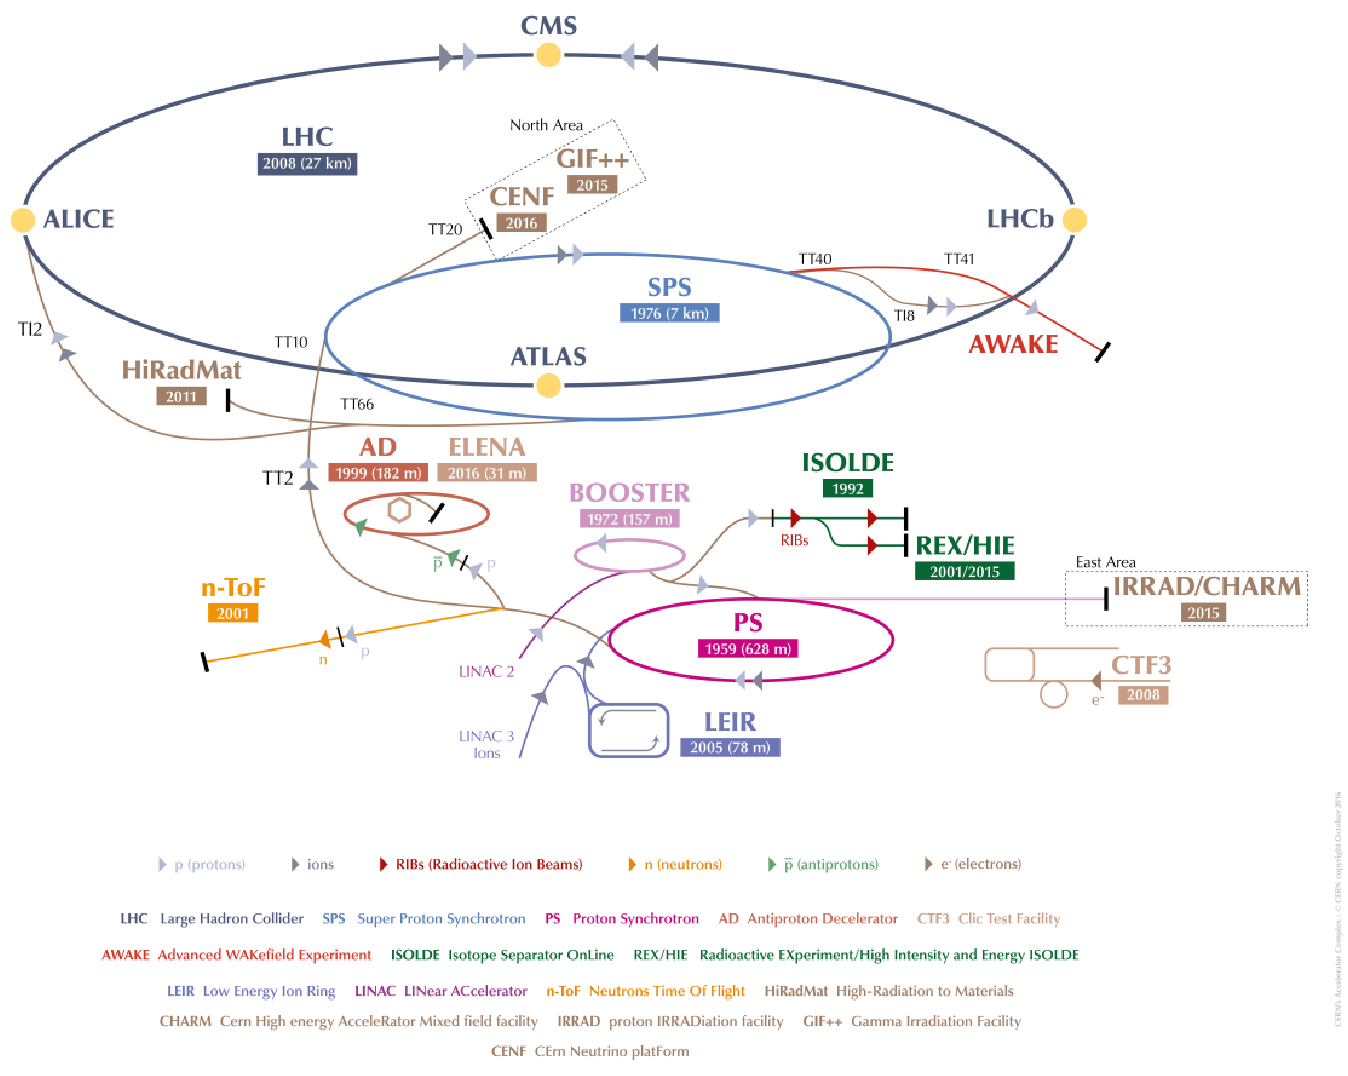
\includegraphics[width=1.0\linewidth]{figs/detector/AccComplexpng2pdf_cropped.pdf}
	\caption{Accelerator complex at CERN. The image is taken from \cite{complex}.}
  \label{fig:AcceleratorComplex}
\end{figure}

\Gls{LHC} is a complex machine which accelerates beams of protons in opposite directions in a $\sim$ 27km long circular tunnel. It is located
50-157\m below ground crossing the border between Switzerland and France. Once the desired energy is achieved proton-proton ($pp$) or ion collisions happen at four distinct points, where different detectors with different physics focus are located. These are \Gls{ATLAS}, \Gls{CMS}, \Gls{ALICE} and \Gls{LHCb}. 
The search for the decay \Bmumumu was performed using data obtained at \Gls{LHCb}. 

\section{LHCb Layout }

\begin{figure}
	\centering
	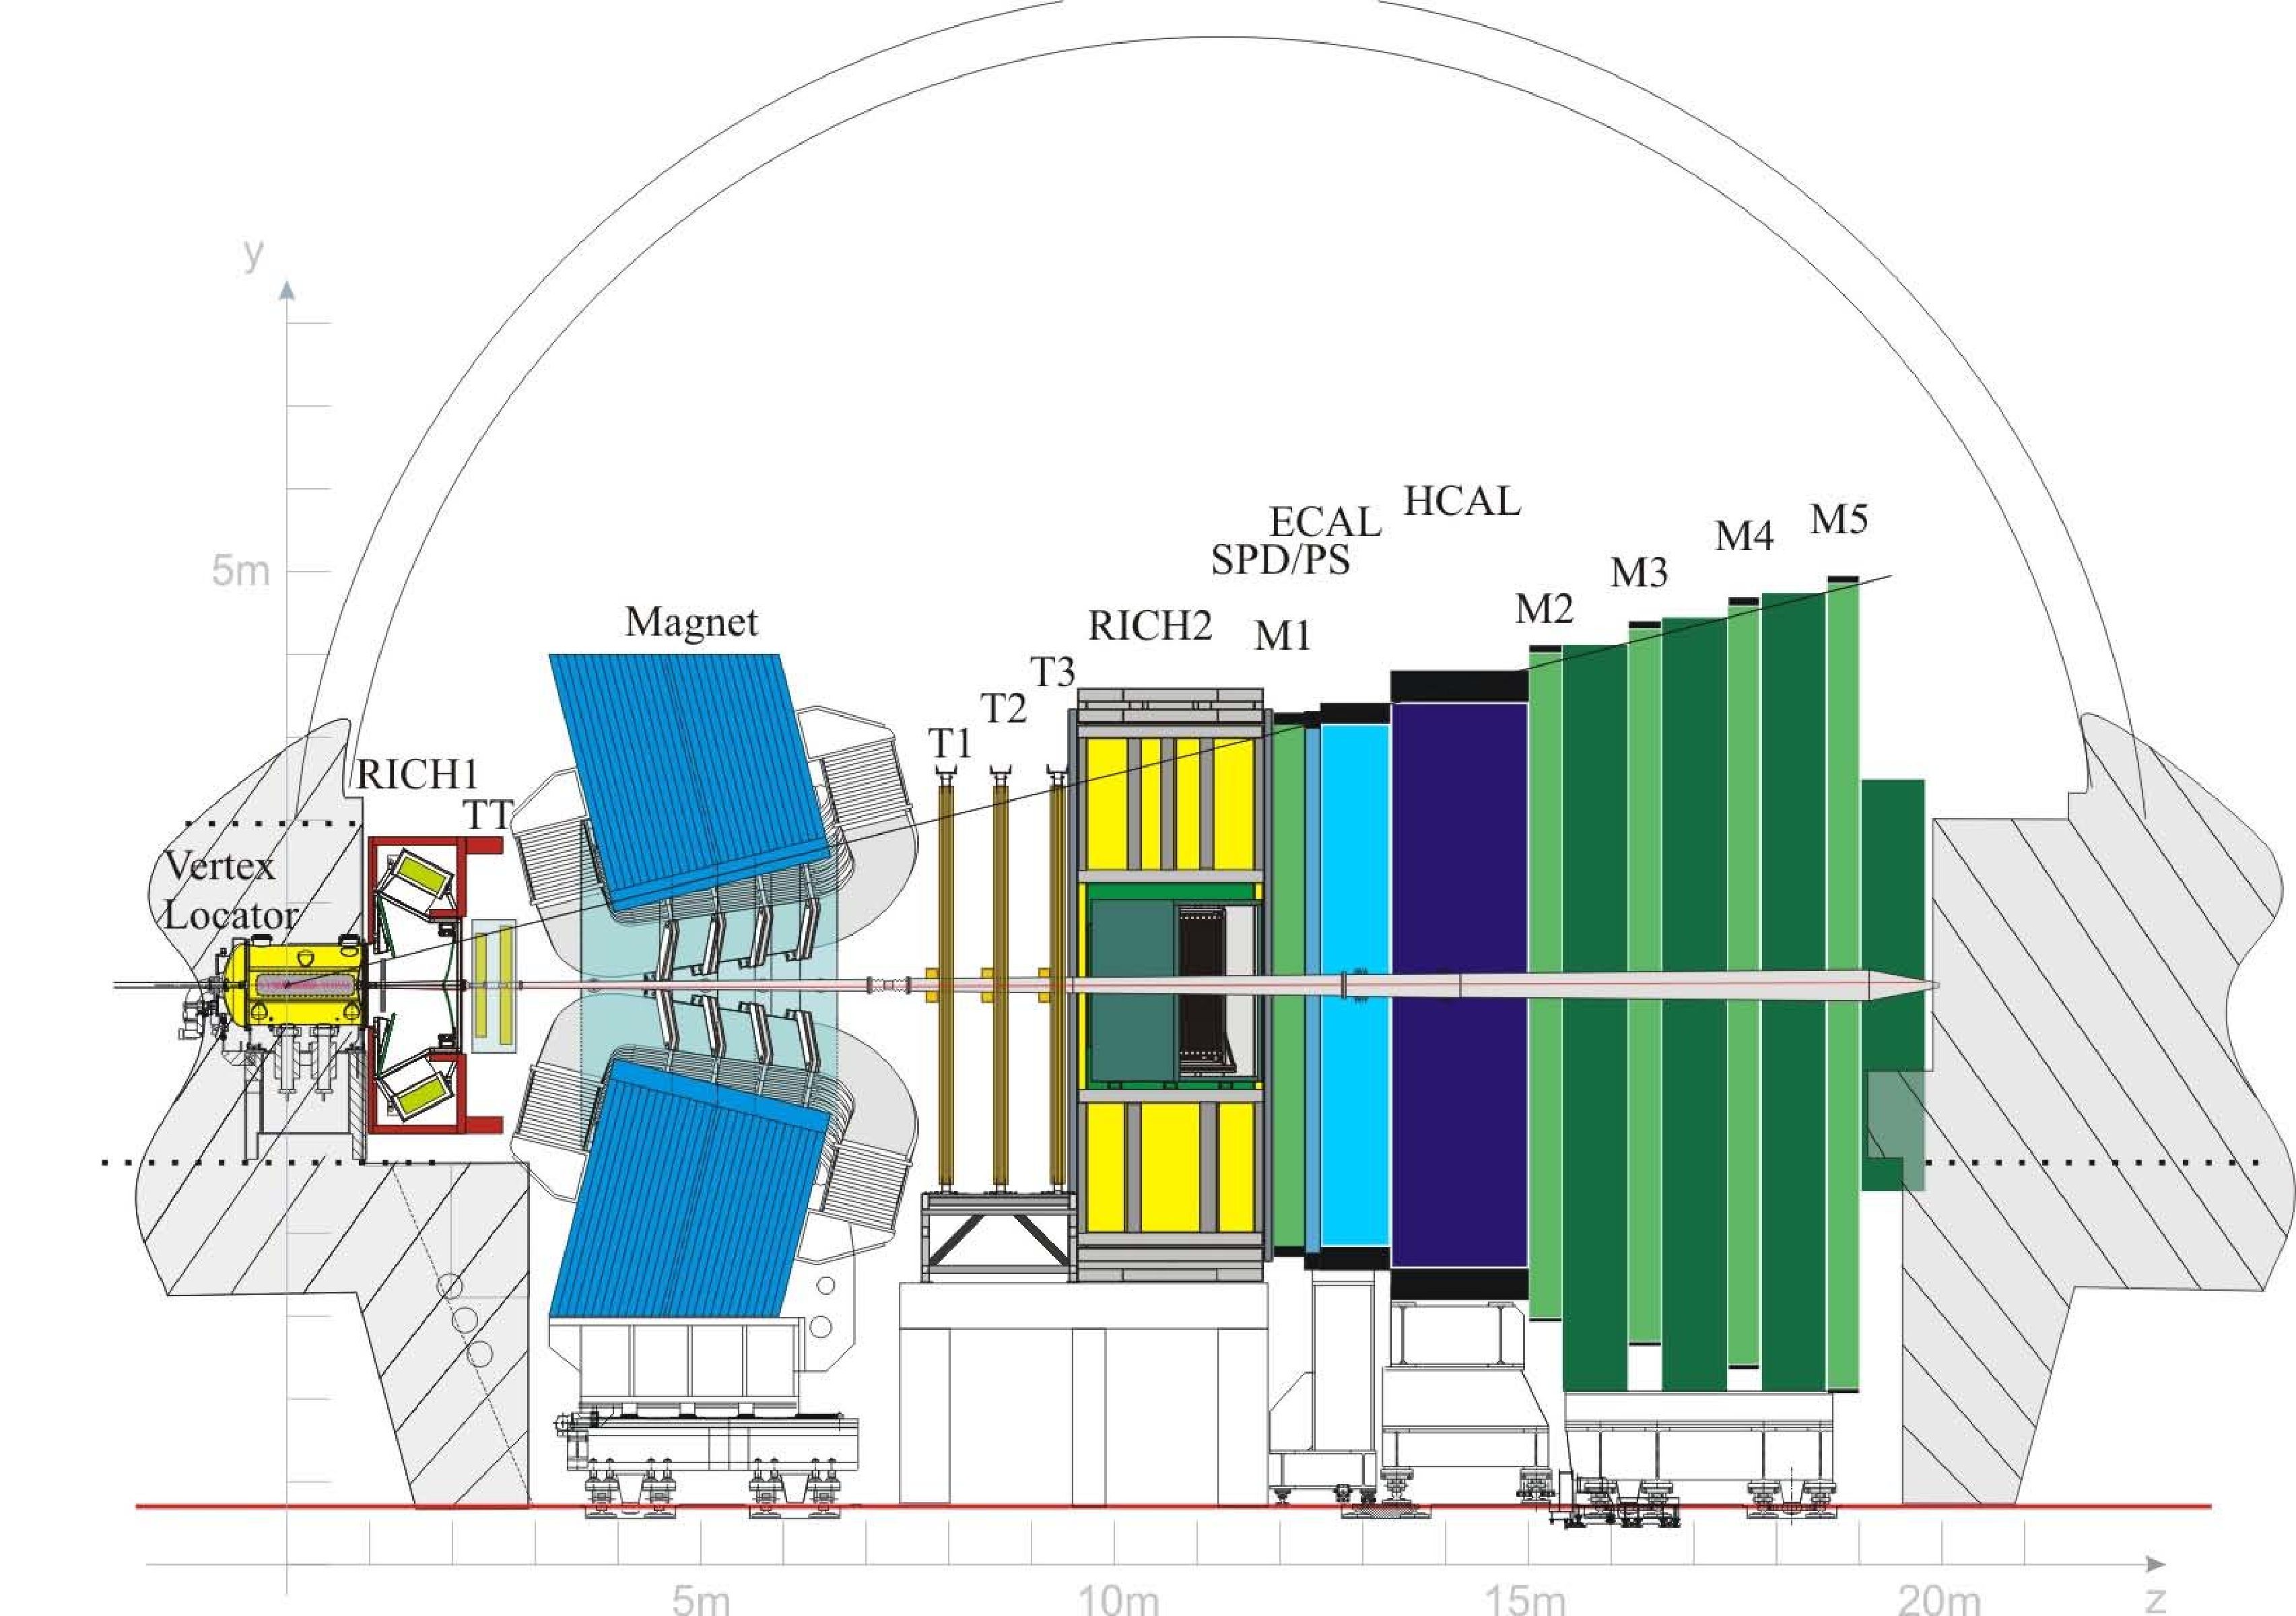
\includegraphics[scale = 0.25]{figs/detector/lhcbdet.pdf}
	\caption{Schematic slice of \Gls{LHCb} detector in the $y,z$ plane where $z$ is defined to be the direction parallel to beamline, and $x,y$ define the plane perpendicular to the beamline. $\theta$, the opening polar in the y-z plane with $\theta$ = 0 along the $z-axis$. Figure from \cite{LHCbdetector}.}
	\label{fig:LHCbDetector}
\end{figure}


\Gls{LHCb}, seen in~\autoref{fig:LHCbDetector}, differs from the other general purpose detectors on the \Gls{LHC} ring as its main aim is to study properties of heavy particles containing $b$ or $c$ quarks. This is possible as this experiments was designed to have the geometrical acceptance and unique vertex resolution as well as excellent particle identification (\Gls{PID}) suitable for beautiful and charming physics.

Studies of $B$ mesons can happen either at positron-electron colliders or at hadron colliders. The advantage of positron-electron collider is that the information about all the event is known, as just two $B$ mesons and nothing else is produced in collisions. This gives an overall constraint on collision information, unlike in the hadron collider $B$ factory, \gls{LHCb}. Contrary to the two general purpose detectors at \gls{LHC}, where the collisions are occurring in the centre of the detector, \Gls{LHCb}'s collision point is located at one end of the detector, hence its description as a forward single-arm spectrometer. 

The disadvantage of not having an overall constraint on collision information is, however, compensated by the production mechanism of $b\bar{b}$ and $c\bar{c}$ in $pp$ interactions, which occurs predominantly via gluon-gluon fusion. In this process, each gluon will carry part of proton's momentum. If the two gluons from two protons carry significantly different momentum, the $b\bar{b}$ system will be boosted with respect to the $pp$ rest frame, either in the forward or backward cone closely to the beamline, as can be seen in~\autoref{fig:Acceptance}(b).


\begin{figure}
	\centering
	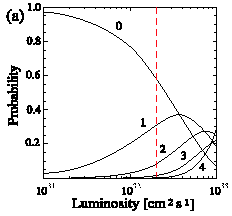
\includegraphics[width=0.45\linewidth]{figs/detector/license/croped.pdf}%
	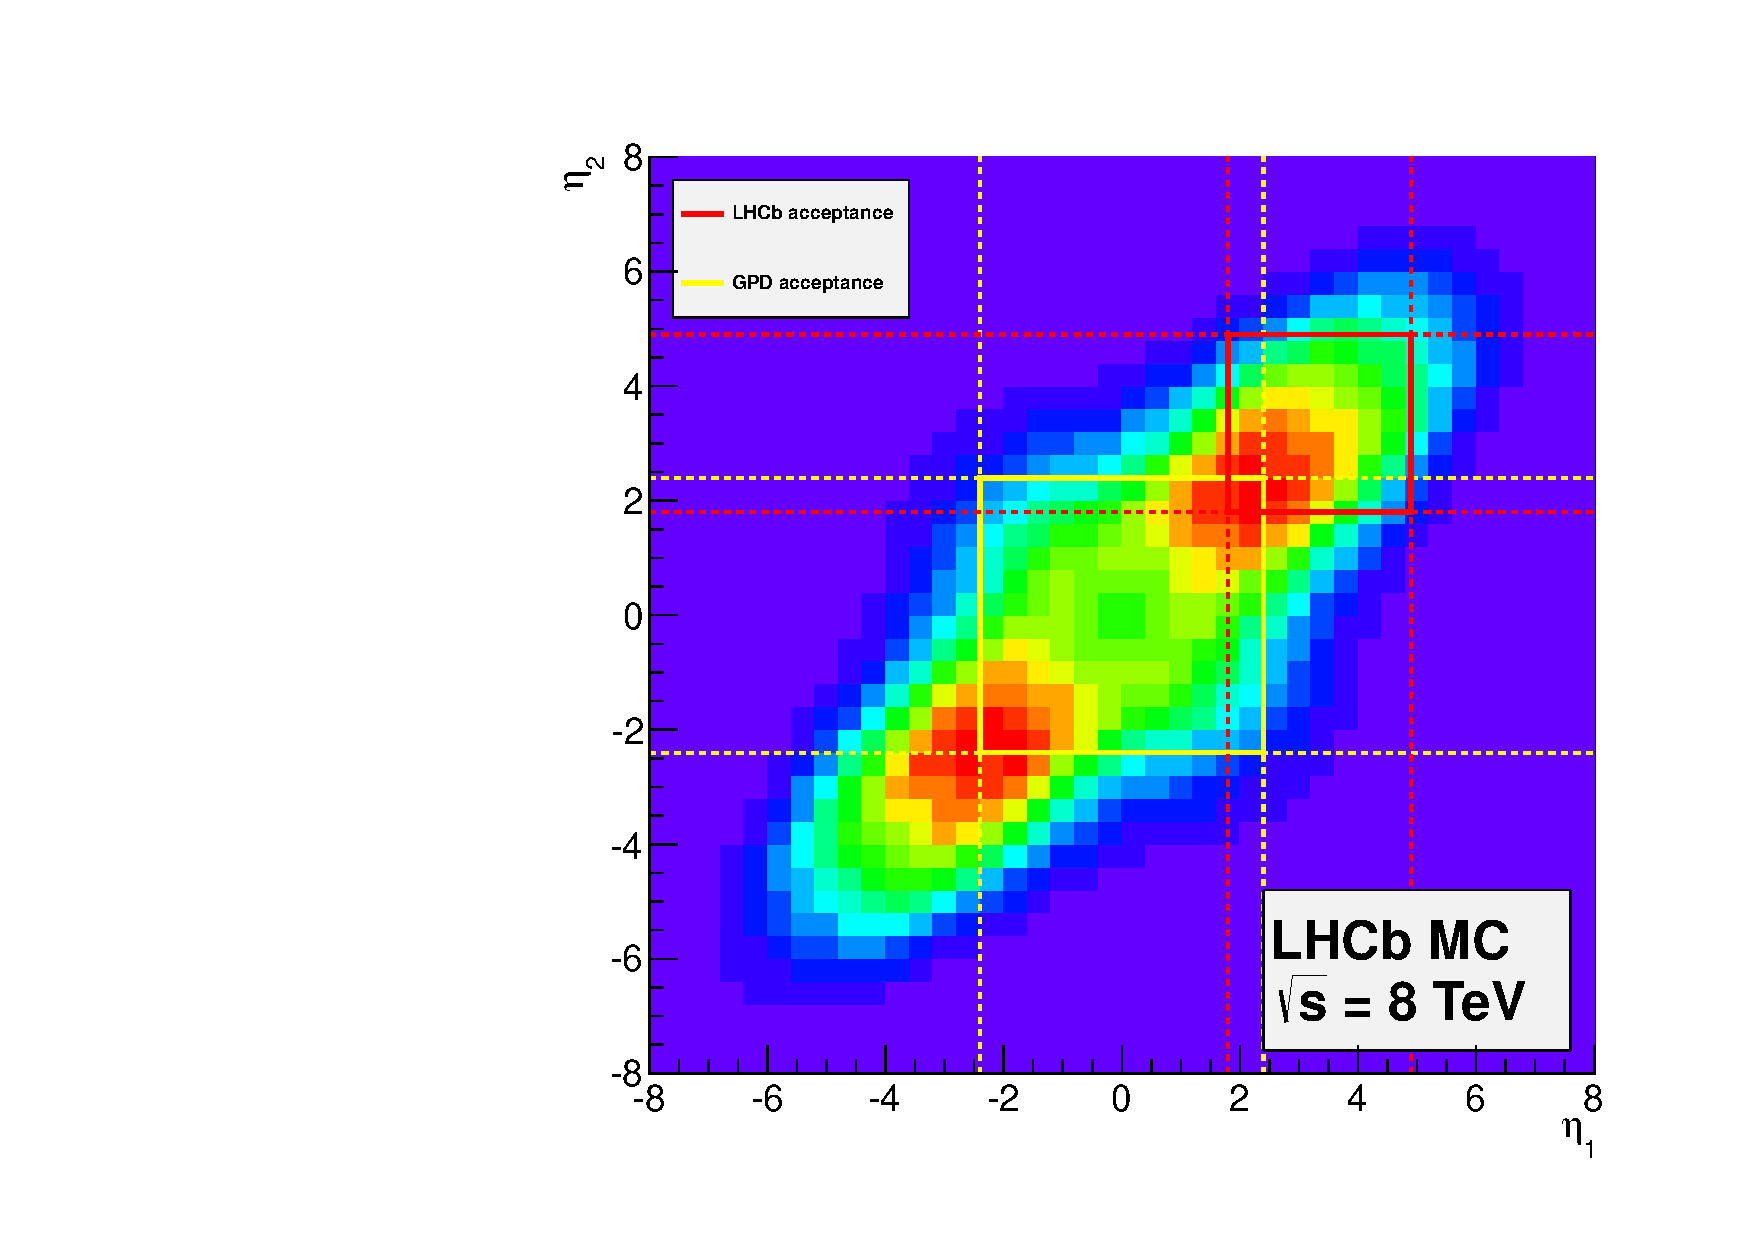
\includegraphics[width=0.5\linewidth]{figs/detector/Acceptance.pdf}\put(-10,170){(b)}
	\caption{(a) Probability of interaction per bunch crossing as a function of instantaneous luminosity. Figure from \cite{Raven:2007zi}. (b) Angular production and acceptance of the $b$ (x-axis) $\bar{b}$ (y-axis) pair produced from $pp$ collision at the LHC. The acceptance of the LHCb detector is the red box and the acceptance of the General Purpose Detector is shown in the yellow box. \Gls{LHCb} covers the region with highest production cross-section at 8 \tev. These plots were produced using a Pythia 8.1 \cite{pythia8} simulation. Figure from \cite{acceptance}.}
	\label{fig:Acceptance}
\end{figure}

The angular coverage of \Gls{LHCb} is formally defined using pseudorapidity $\eta$, 

\begin{equation}
	\eta = -\ln \Big(\tan\frac{\theta}{2}\Big)
\end{equation}	
where $\theta$ is the polar angle measured from the beam axis. The \Gls{LHCb} detector was built to cover the region $2<\eta<5$. The production cross-section of the fundamental process of $pp\rightarrow b\bar{b}X$ was measured in this region yielding, $\sigma (pp\rightarrow b\bar{b}X)$= 75.3$\pm$5.4$\pm$13.0 $\mub$ at 7 \tev \cite{LHCb-PAPER-2010-002} and 144$\pm$1$\pm$21 $\mub$ at 13 \tev \cite{LHCb-PAPER-2016-031}, which shows that the production cross-sections scales roughly linearly with the centre-of-mass energy. Assuming design conditions of \gls{LHCb}, listed in~\autoref{tab:runcond}, 2$\fb^{-1}$ of data (eqvivalent to 2012 dataset) would correspond to $10^{12}$ of $b\bar{b}$ pairs being produced in a full 4$\pi$ region with 27\% of these $b\bar{b}$ pairs produced in the \gls{LHCb} acceptance. The summary of \gls{LHCb} running conditions is also provided in~\autoref{tab:runcond}. The analysis of \Bmumumu is done with Run \Rn{1} and 2016 dataset. 

Despite the impressive statistics of $b\bar{b}$ pairs available to \Gls{LHCb}, the bottleneck in terms of data collection arises from the much more copious inelastic background. That mostly originates from soft \gls{QCD} processes which are related to the amount of pile-up, the visible number of $pp$ interaction in the visible events. By looking at the probability of the number of $pp$ interaction per bunch crossing as a function of luminosity, shown in~\autoref{fig:Acceptance}(a), it can be noted that the maximum probability for only one $pp$ interaction (and hence minimizing the background) is found to be at $\sim 2 \times10^{32} \mathrm{cm^{-2} s^{-1}}$.  This was the reason behind \gls{LHCb} design luminosity. Subsequently it has been found that it is more optimal to run at a higher luminosity of $\sim 4 \times10^{32} \mathrm{cm^{-2} s^{-1}}$ but then implement a set of global event cuts (GEC). Only events with 600 (in 7,8 \tev) and 450 (in 13 \tev) hits and less, corresponding to the track density in the particular part of the detector, are allowed to be processed.
As the majority of the branching fractions at \gls{LHCb} are measured with respect to other branching fractions, there is no bias being introduced by the GECs. 

As \Gls{LHCb} requires much lower luminosity compared to other \gls{LHC} detectors, there is an LHCb-specific control of luminosity known as \textit{luminosity levelling}, shown in~\autoref{fig:lhcbintlumi}. This procedure achieves stable instantaneous luminosity by controlling that the two beams do not collide straight head-on at collision point, but are moved with respect to each other. It limits the effects of luminosity decay, which can lead to trigger alterations during specific data taking run, resulting in systematic uncertainties.



%The summary of \gls{LHCb} running conditions is provided in~\autoref{tab:runcond}, showing the evolution of the instantaneous luminosity as well as the frequency of collisions compared to the design proposal.
%Formally \Gls{LHCb}   detector is placed along the beamline, where $x,y,z$ a spectrometer which cover the region of 300 \mrad defined a
%http://lhcb.web.cern.ch/lhcb/speakersbureau/excel/default.html

%\begin{figure}
%	\centering
%	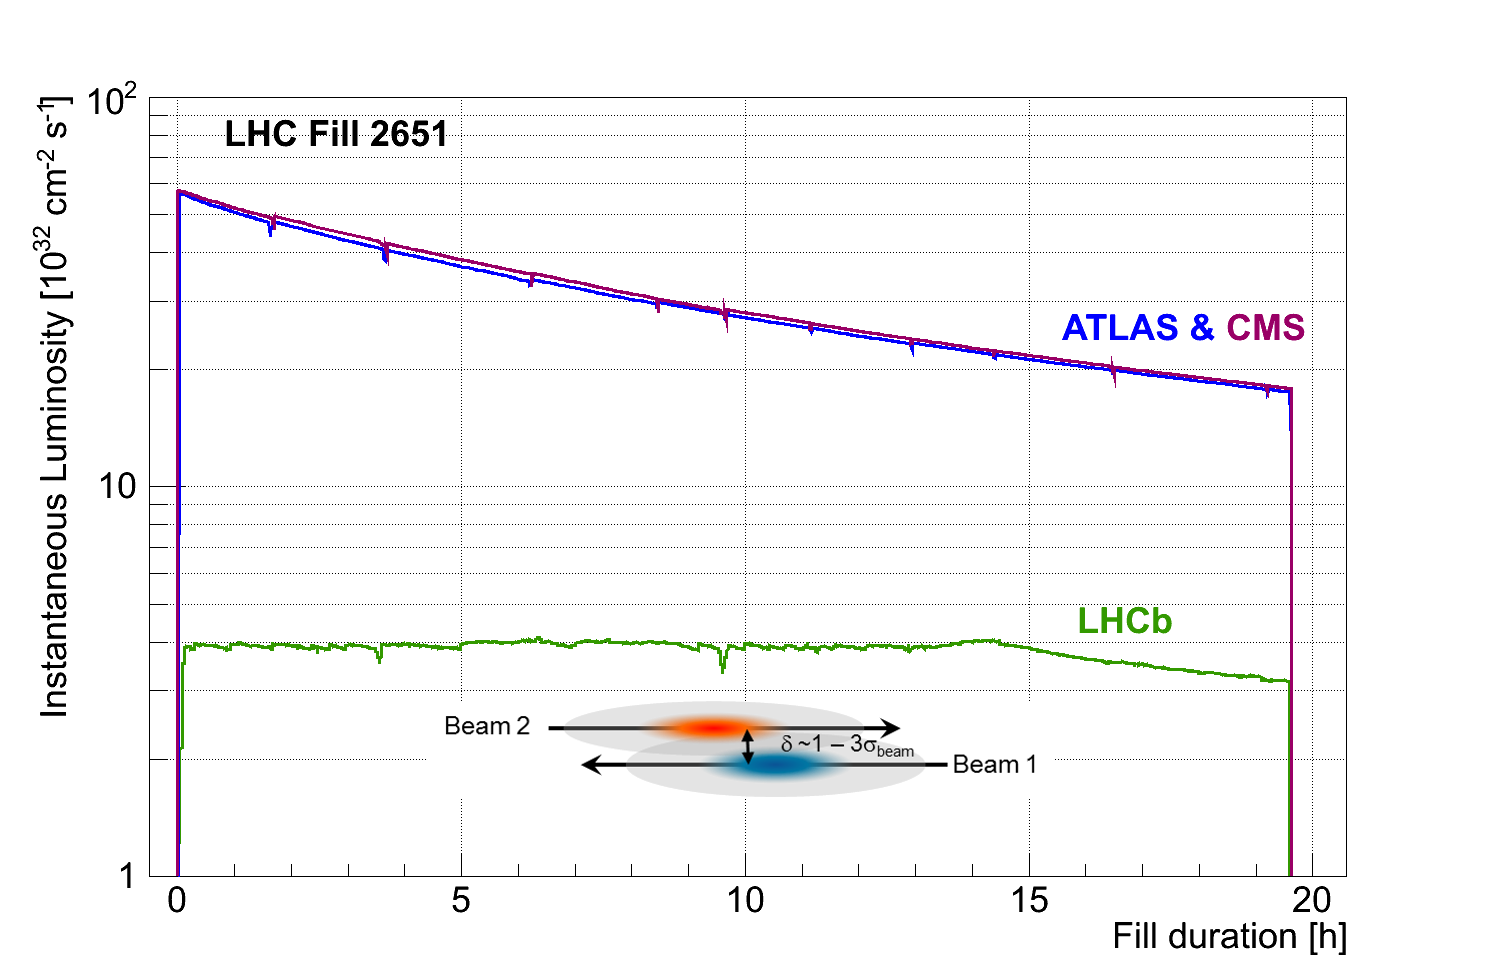
\includegraphics[scale = 0.5]{figs/detector/lumicompare.png}
%	\caption{Integrated luminosity collected in different years of data-taking. This plot is taken from \cite{lumiover}.}
%	\label{fig:lhcbintlumi}
%\end{figure}



\begin{table}[!h]
	\centering
%	\hspace*{-0.8cm}
	\begin{tabular}{l c c c }
		\toprule
		Year & $\sqrt{s}$ & $\mathcal{L}$  & Integrated Recorded Luminosity \\ 
		 & [\tev] & [$\times10^{32} \rm{cm^{-2}s^{-1}}$] & [$\rm{fb}^{-1}$] \\ \hline
		Design & Up to 14 & 2 & - \\
		2011  \rdelim\}{2}{1.5cm}[Run \Rn{1}] & 7 & $\sim$ 3.0-3.5 & 1.1 \\
		2012 & 8 & $\sim$ 4.0 & 2.1 \\
		2015 \rdelim\}{3}{1.5cm}[Run \Rn{2}] & 13 & $\sim$ 0.5-4.5 & 0.3 \\      
		2016 & 13 & $\sim$ 4.0 & 1.7  \\      
		2017 & 13 & $\sim$4.0-6.0 & 1.7 \\\bottomrule      
	\end{tabular}
	\caption{Running conditions of \gls{LHC} and \Gls{LHCb} in different years of data-taking. The statistics of \gls{LHCb}'s instantaneous luminosity, $\mathcal{L}$ is extracted using run database information. Run \Rn{2} data-taking finishes in 2018.}
	\label{tab:runcond}
\end{table}   

\begin{figure}
	\centering
%	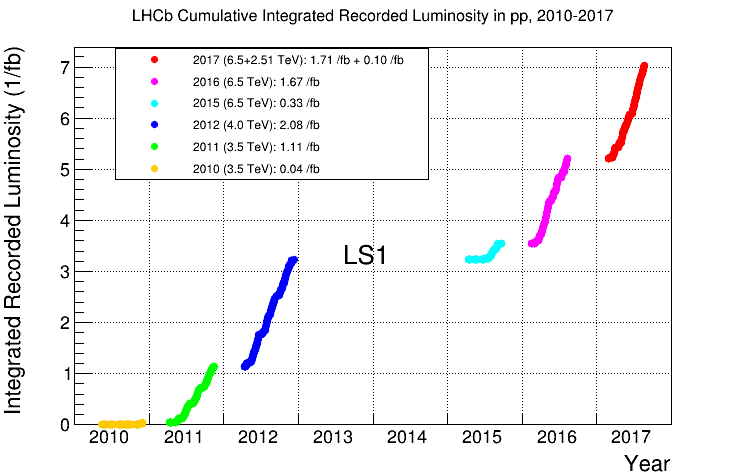
\includegraphics[width = 0.5\textwidth]{figs/detector/intlumi.png}\put(-15,100){(a)}
        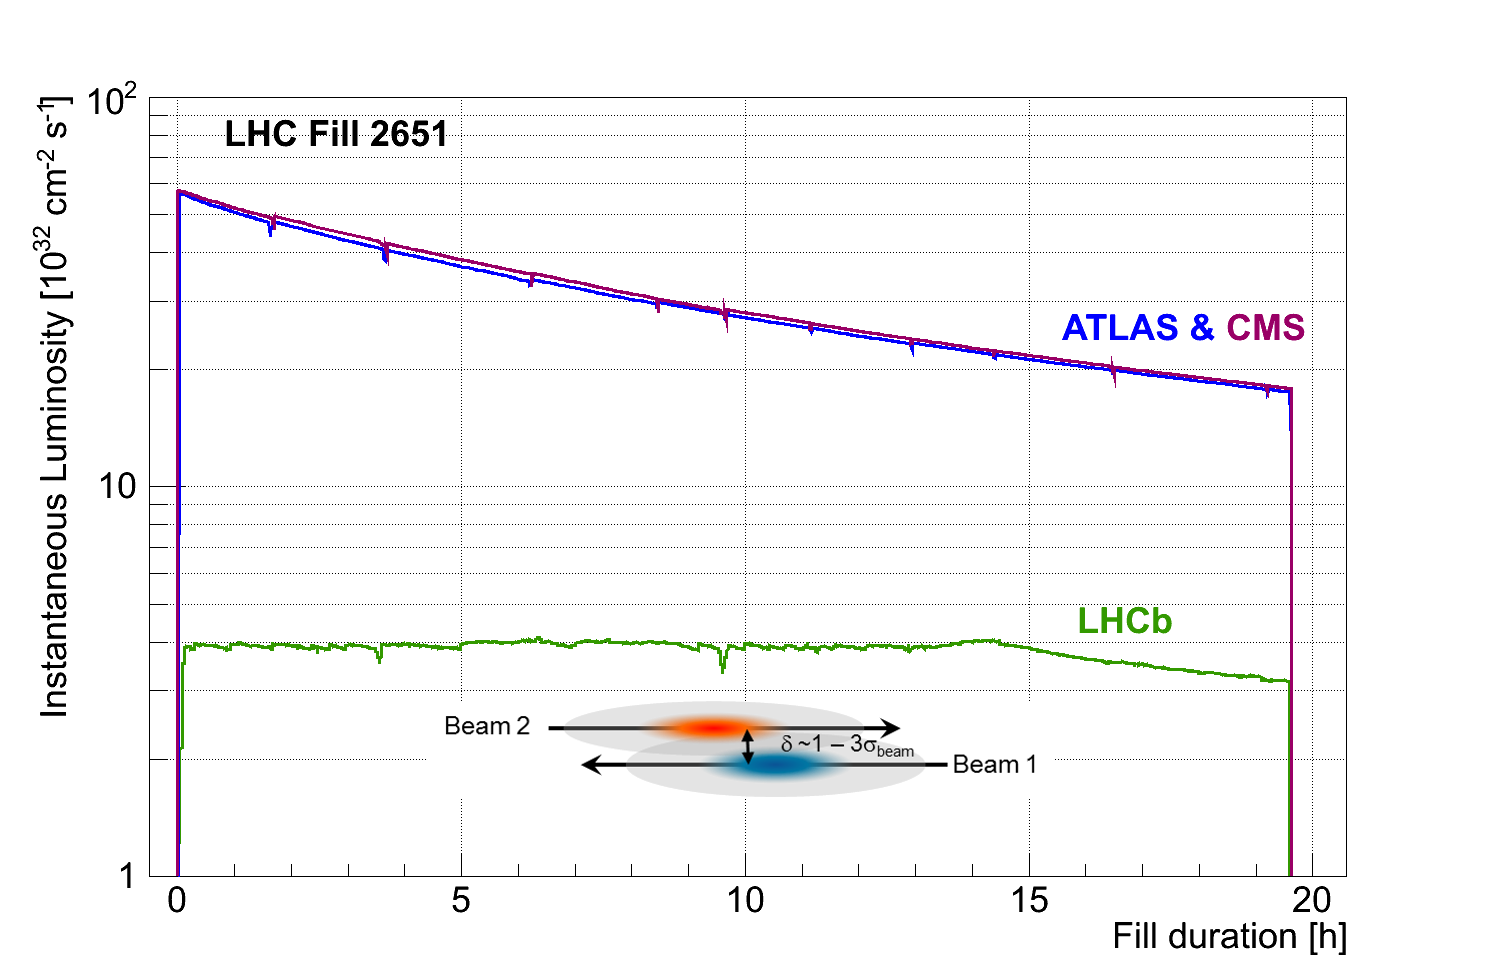
\includegraphics[width = 0.65\textwidth]{figs/detector/lumicompare.png}%\put(-15,100){(b)}
	%\caption{(a) Integrated luminosity collected in different years of data-taking. This plot is taken from \cite{lumiover}. (b)
	\caption{Development of the instantaneous luminosity for \Gls{ATLAS}, \Gls{CMS} and \Gls{LHCb} during LHC fill 2651. After ramping to the desired value of $4\times10^{32}\mathrm{cm^{-2}s^{-1}}$
	for \Gls{LHCb}, the luminosity is kept stable in a range of 5$\%$ for about 15 hours by adjusting the transversal beam overlap. The difference in luminosity towards the end of the fill between \Gls{ATLAS}, \Gls{CMS} and \Gls{LHCb} is due to the difference in the final focusing at the collision points, commonly referred to as the beta function, $\beta^{*}$. This plot was obtained from \cite{LHCb-DP-2014-002}.}
	\label{fig:lhcbintlumi}
\end{figure}

In the following sections, a brief discussion of the different subdetectors, shown in~\autoref{fig:LHCbDetector}, is presented. The vertexing at \gls{LHCb} is performed with the vertex locator system, also known as the VELO, is described in~\autoref{velosys}. The tracking system at \gls{LHCb} consisting of trackers before magnet (TT), and three tracking stations behind the magnet (T1, T2, T3) is highlighted in~\autoref{tracksys}. The particle identification is provided by two Ring Imaging \v{C}erenkov counters (RICH1 and RICH2), which are detailed in~\autoref{richsec}. No particle physics experiment is complete without a calorimeter system, discussed in~\autoref{calosys}, which consists of a Scintillator Pad Detector (SPD), Preshower (PS), an electromagnetic calorimeter (ECAL) and finally a hadronic calorimeter (HCAL). The muon system positioned at the end of the detector, consisting of five muon chambers is described in~\autoref{muonsys}. The trigger chain as well as the simulation chain are discussed in~\autoref{triggerchap} and~\autoref{simulationchap}. Particular emphasis is given to the muon detectors and the simulation of \gls{LHCb}.

%\color{red}{ \mybox{Sally} corrected until now} \color{black}.

\section{VErtex LOcator }
\label{velosys}
The subdetector closest to the collision point is the VErtex LOcator (\Gls{VELO}). This silicon-strip based detector, that extends 1 \m along the beam axis, is primarily used to distinguish signal-like events from prompt background. The typical differing property of a $b$-hadron decay includes large impact parameter (\Gls{IP}), the minimal distance between the track and a  primary vertex, in addition to significantly higher transverse momentum, $p_{T}$. Therefore, the main tasks of this subdetector is to find: 
\begin{itemize}
\item primary vertices positions
\item secondary vertices of short-lived particles (heavy quark hadrons)
\item tracks that did NOT originate from primary vertex
\end{itemize}.


\begin{figure}[!h]
	\centering
	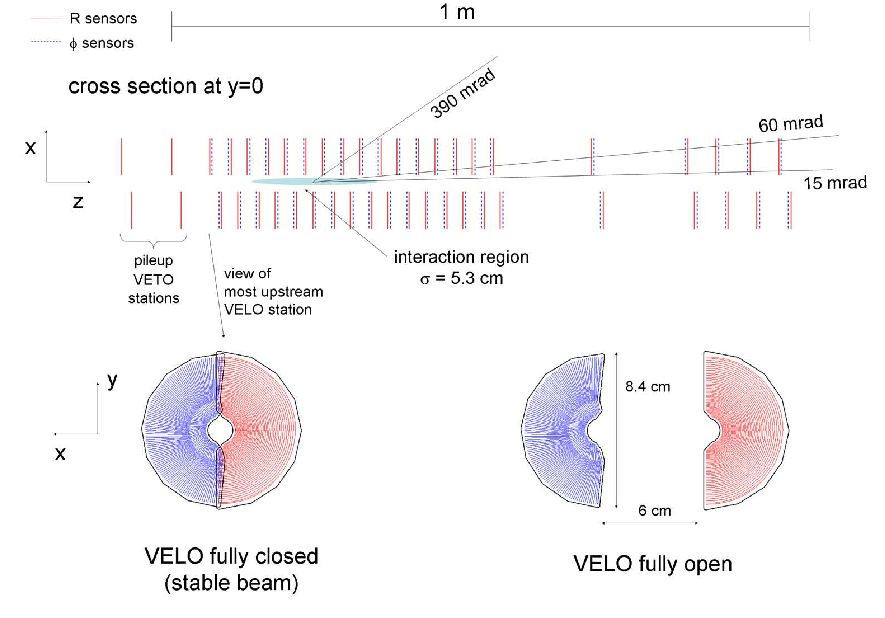
\includegraphics[width = 0.75\textwidth]{figs/detector/license/Velo_croped.pdf}
        %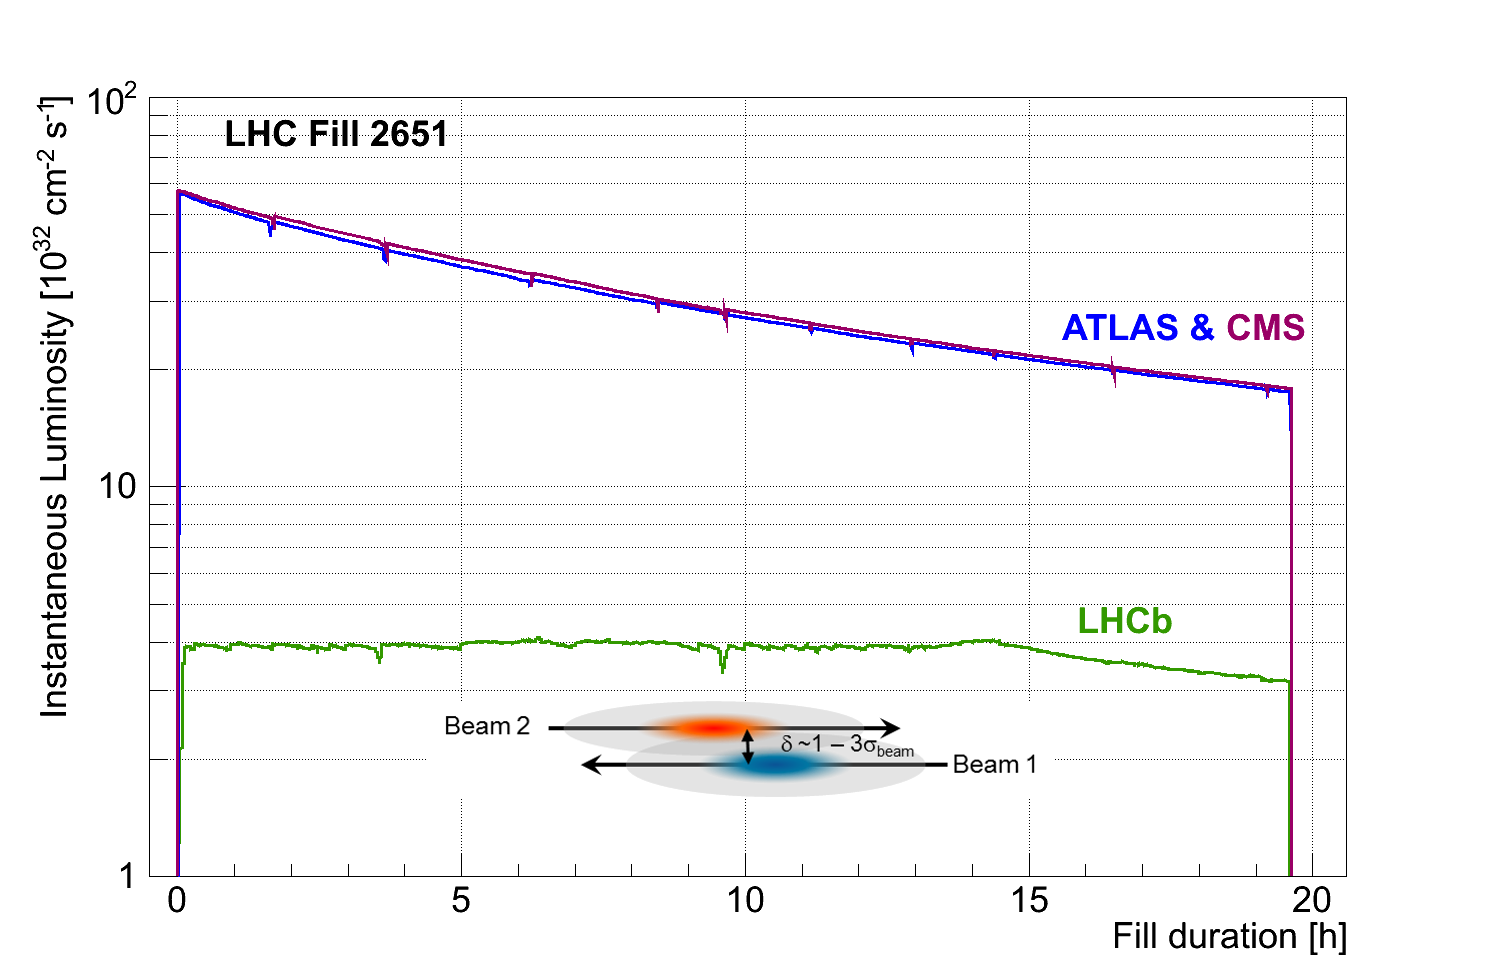
\includegraphics[width = 0.5\textwidth]{figs/detector/lumicompare.png}
	\caption{Schematic plot of the \Gls{VELO} detector configuration along the beam pipe showing the layout as well as positions while in stable beams (discs have slight overlap) and injection. Figure from \cite{det_paper}.}
	\label{fig:veloover}
\end{figure}

The detector consists of two sets of 21 silicon modules positioned around the beam pipe, where each module has 2 types of half-moon-shaped discs as seen in~\autoref{fig:veloover}. In the first type, the strips are arranged to provide radial information ($R$), whereas the second type provides azimuthal ($\phi$) information. As $pp$ collisions bring a high dose of radiation to this detector, the first sensitive strip starts at a distance of 8 \mm once stable beams are declared. Throughout the beam injection, when the beam radius may be larger, the two sets are moved 3 \cm away, perpendicular to the beam axis. For the $R$ sensor, the individual module's strip pitch, the distance between two strips, varies from 38 $\mum$ to 102 $\mum$ away from the beam pipe, so that the hit occupancy is roughly even as a function of distance away from the beam pipe. Each \Gls{VELO} half is kept within an aluminium welded box causing material overlap once stable beams are declared. These boxes form their own vacuum which is separated from the nominal \gls{LHC} vacuum in order to protect the detector from any electromagnetic interference with the beam. 

This setup brings outstanding hit resolution (4-40$\mum$), which in turn allows for very high \gls{IP} and very good primary vertex (\gls{PV}) resolution, as seen in~\autoref{fig:veloIPres}(a)(b). This is indispensable not only in order to perform the precise measurements of $B$ and $D$ lifetimes, but also to resolve oscillations caused by $B^{0}_{s}-\bar{B}^{0}_{s}$ mixing occurring at a 3 trillion \hz rate. As will be seen later, this excellent resolution is also very important for the detection of decays with neutrinos in the final state.

\begin{figure}[!h]
	\centering
	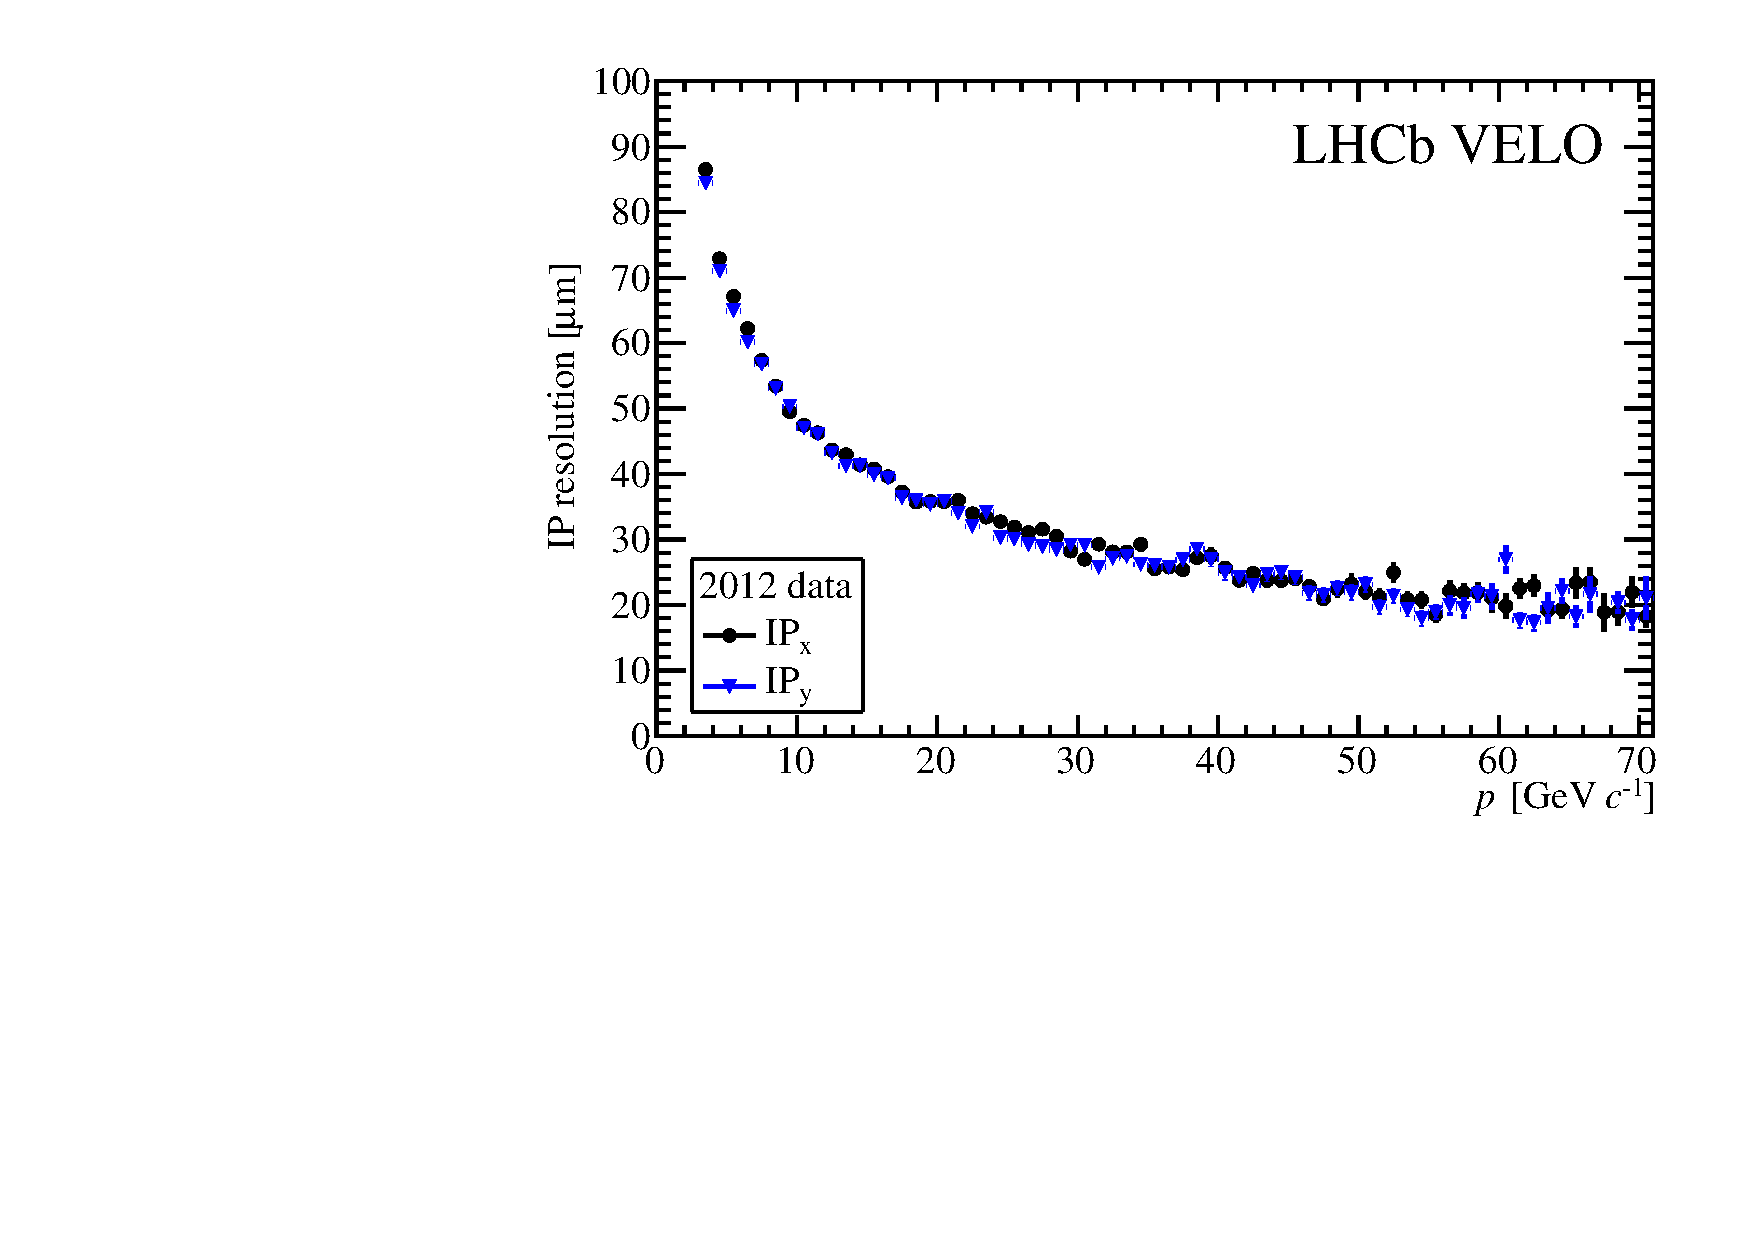
\includegraphics[width = 0.5\textwidth]{figs/detector/IPRes-Vs-P-CompareIPxIPy-2012.pdf}\put(-50,70){(a)}
        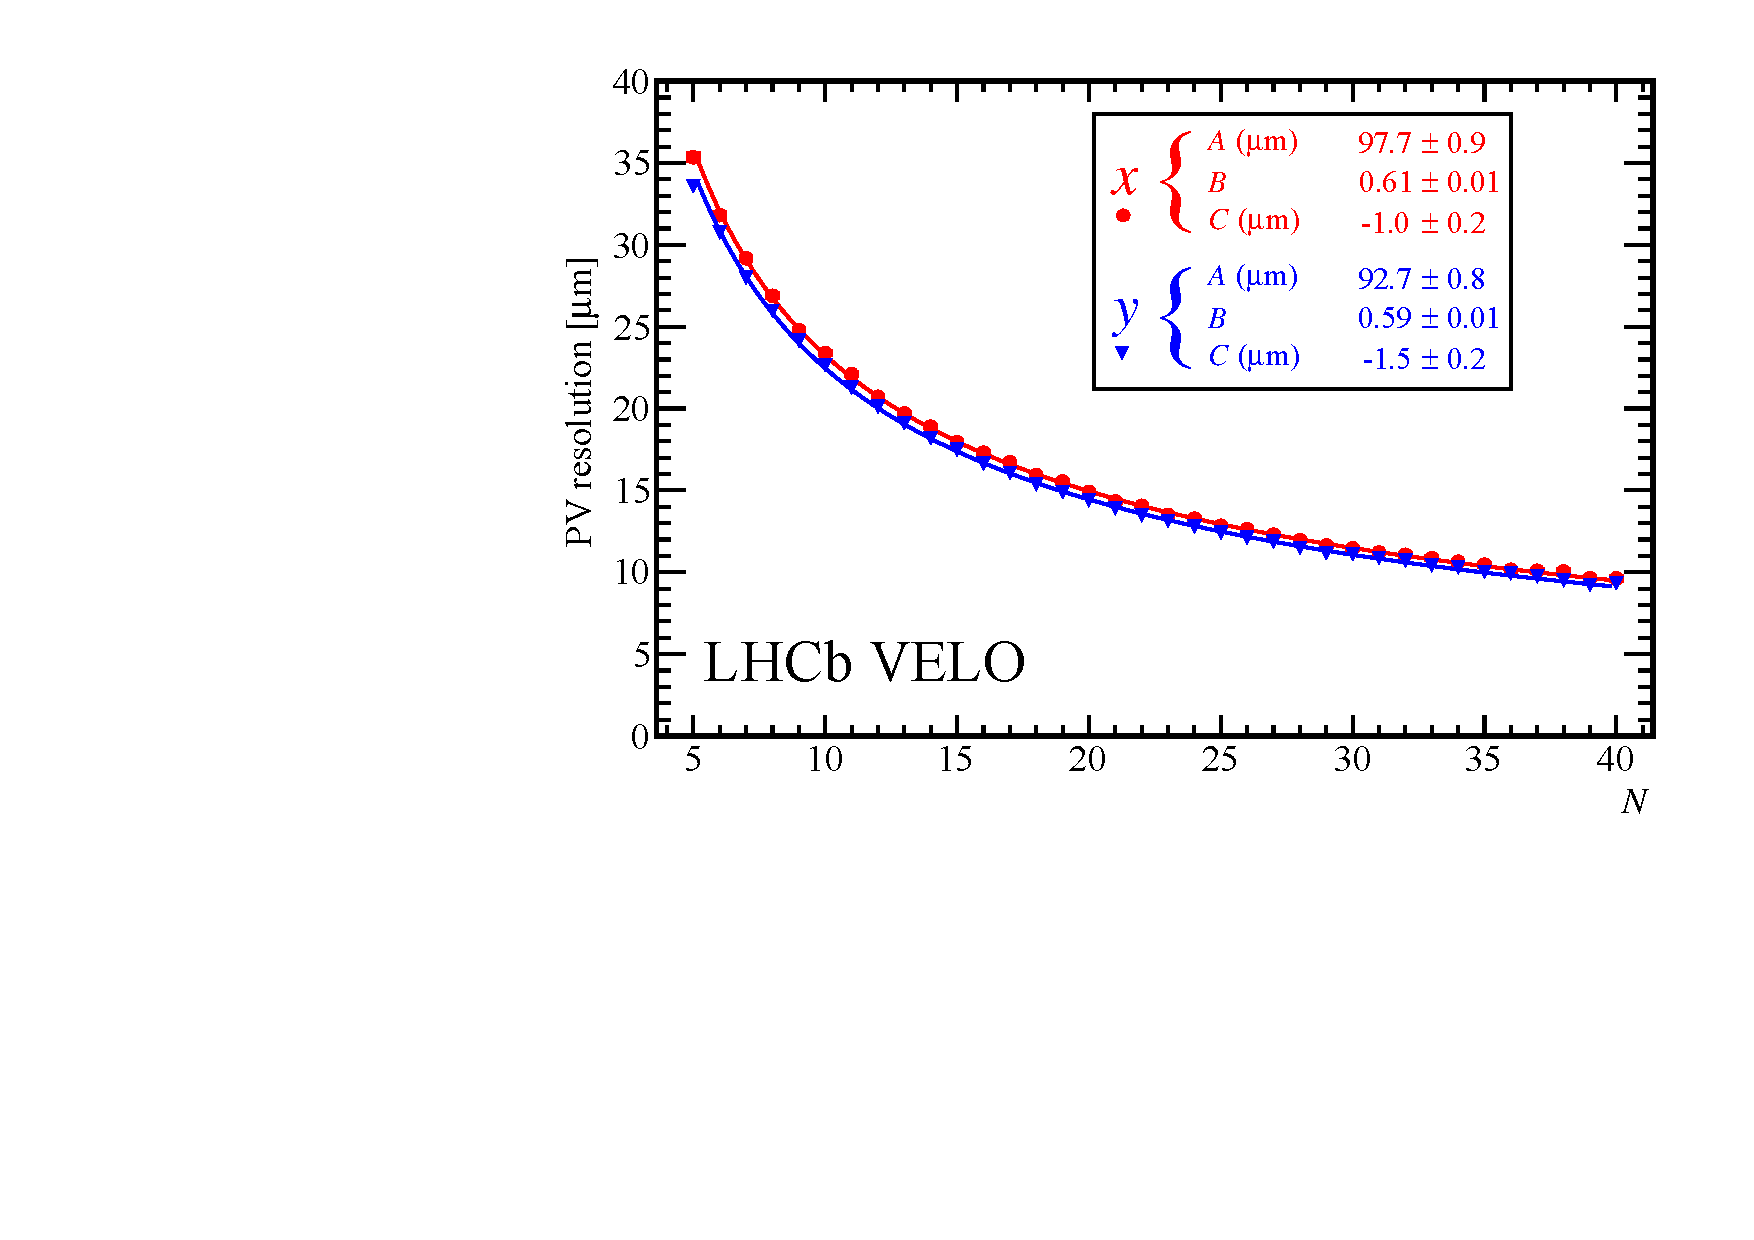
\includegraphics[width = 0.5\textwidth]{figs/detector/ResXY_1PV_2011Data.pdf}\put(-50,70){(b)}
	\caption{Two key variables which quantify performance of the \Gls{VELO} detector. (a) \Gls{IP} resolution which is worse for low momentum tracks and (b) \Gls{PV} resolution dependent on the number of tracks forming the primary vertex $N$. Figures from \cite{LHCbVELOGroup:2014uea}.}
	\label{fig:veloIPres}
\end{figure}


\section{Tracking System }
\label{tracksys}
In addition to tracking information provided by the \Gls{VELO}, the trajectories of charged particles are measured by a series of tracking subdetectors. The main task of these tracking subdetectors is to provide efficient reconstruction and precise measurement of a particle's momentum. There are four tracking stations apart from \Gls{VELO}: Tracker Turicensis (\Gls{TT}), positioned upstream from the magnet, and the \Gls{Tstation} tracking stations on the other side of the magnet. The dipole magnet with $\approx$ 4 Tm integrated field provides strength to bend charged particles in horizontal plane.
% 10 m of charged trakcs
%with $p$ of 200 $\gev/c^{2}$.      

 Two different detection technologies are used in these trackers reflecting the nature of track occupancy as a function of polar angle. The tracker's part at small polar angles, \Gls{TT} station together with central region of \Gls{Tstation}, also known as Inner Tracker (\Gls{IT}), expects higher occupancy and makes use of the silicon microstrip detection mechanism. The outer part of \Gls{Tstation} stations, also known as the Outer Tracker (\Gls{OT}), is made of straw-tube detectors. Straw tubes measure the trajectory of the track by measuring the drift-time of ionized electrons. Use of the two technologies is illustrated in~\autoref{fig:tracktype}(a). 

\subsection{Tracking Algorithms} 
Different types of particles will leave different footprints in the detector. Charged particles will form tracks. Depending on the presence of hits in individual subdetectors, they are grouped into several categories, visualized in~\autoref{fig:tracktype}(b).

\begin{figure}[!h]
	\centering
	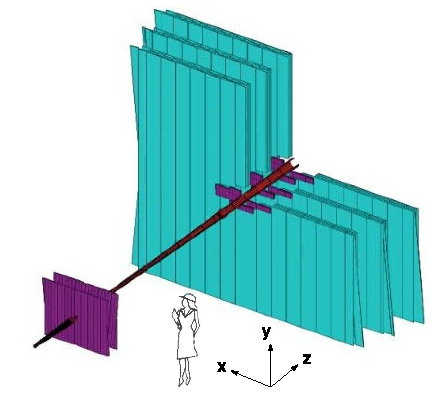
\includegraphics[width = 0.35\textwidth]{figs/detector/license/OT_crop.pdf}\put(-30,90){(a)}%
	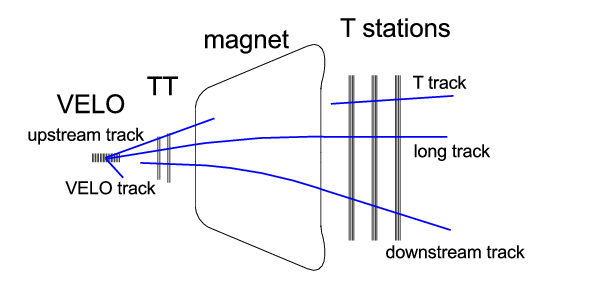
\includegraphics[width = 0.6\textwidth]{figs/detector/tracktype.png}\put(-30,90){(b)}
	\caption{ (a) Visualisation of use of different technology with silicon technology in violet and straw-tube technology in cyan. Figure from \cite{det_paper}. (b) Track types categorisation depending on which track stations provided hits. For the study of \Bmumumu decays, only \gls{longtrack}s are considered as muons will travel to the end of the detector leaving the hits all along. Figure from \cite{LHCb-DP-2013-002}.}
	\label{fig:tracktype}
\end{figure}

%http://iopscience.iop.org/article/10.1088/1748-0221/3/08/S08005/pdf
%https://twiki.cern.ch/twiki/bin/view/LHCb/TrackingEffAbsLength /secondary interactions - hadronic int.

Most of the physics analyses at \gls{LHCb}, as it is the case for the search of \Bmumumu, use only \gls{longtrack}s, tracks leaving hits in the \Gls{VELO} and \Gls{Tstation}, as they give most precise momenta measurements. There are also other types of tracks as indicated in~\autoref{fig:tracktype} but they are rarely used.
%VELO tracks leave hits only in $R$ and $\Phi$ sensor, but not in any other tracking stations. VELO tracks are formed by particles which must have left \Gls{LHCb} acceptance or they come from particles produced backwards and hence are useful for \gls{PV} reconstruction. Upstream tracks are formed by tracks leaving hits in \Gls{VELO} and \gls{TT} only. These are usually low momentum particles, which are bent out \Gls{LHCb} acceptance while traversing the magnet. Long-lived particles such as $\Lambda$ or $K^{0}_{s}$ will only decay outside of the \Gls{VELO} acceptance and hence will produce no hits until \Gls{TT} and \Gls{Tstation} forming downstream tracks. T-track is track type that only have hits in \Gls{Tstation}. Again this could be due to presence of long-lived particles or due to secondary interactions in the detector.   

In general, the track reconstruction software starts with \textit{pattern recognition}, where several hits in one part of a tracking subdetector are identified and form \textit{track seeds}, which are then extrapolated and combined with hits in other tracking subdetectors. The long track candidates are formed and fitted with a Kalman filter\cite{Hierk:684697}, where, because of the material present in the detector, corrections for energy losses as well as multiple scattering are incorporated.

In \gls{LHCb} there are types of tracks which are not really the trajectories of charged particles.
Sometimes the \textit{pattern recognition} may combine random hits into a track, which is then known as a \textit{ghost track}. On the other hand, it could also happen that several tracks are sharing the same hits, known as \textit{clone tracks}. The presence of these types of tracks are suppressed through the use of a neural network based variable (\Gls{pgh2}), which relies on $\chi^{2}$ of the track fit, and information about missing hits along the trajectory to calculate its value.
%Presence of these tracks are heavily suppressed with different techniques - such as establishing ghost probability (\Gls{pgh2})- variable based on the output of neural network combining track $\chi^{2}$, quality of the track, and missing hits in the subdetectors.

When searching for a $b$-hadron decay, the mass of a candidate can be calculated from the 4-momenta of the decay products. Uncertainty on this mass is one of the crucial parameters to minimize as it enables a better separation between the identified signal and background. It strongly correlates with momentum resolution that is obtained using tracking system. Resulting relative momentum uncertainty (0.5-1.1\%) on \gls{longtrack}s using $J/\psi \rightarrow \mu^{+} \mu^{-}$ data can be seen in~\autoref{fig:momres}. It varies logarithmically with increasing momentum.


\begin{figure}[!h]
	\centering
	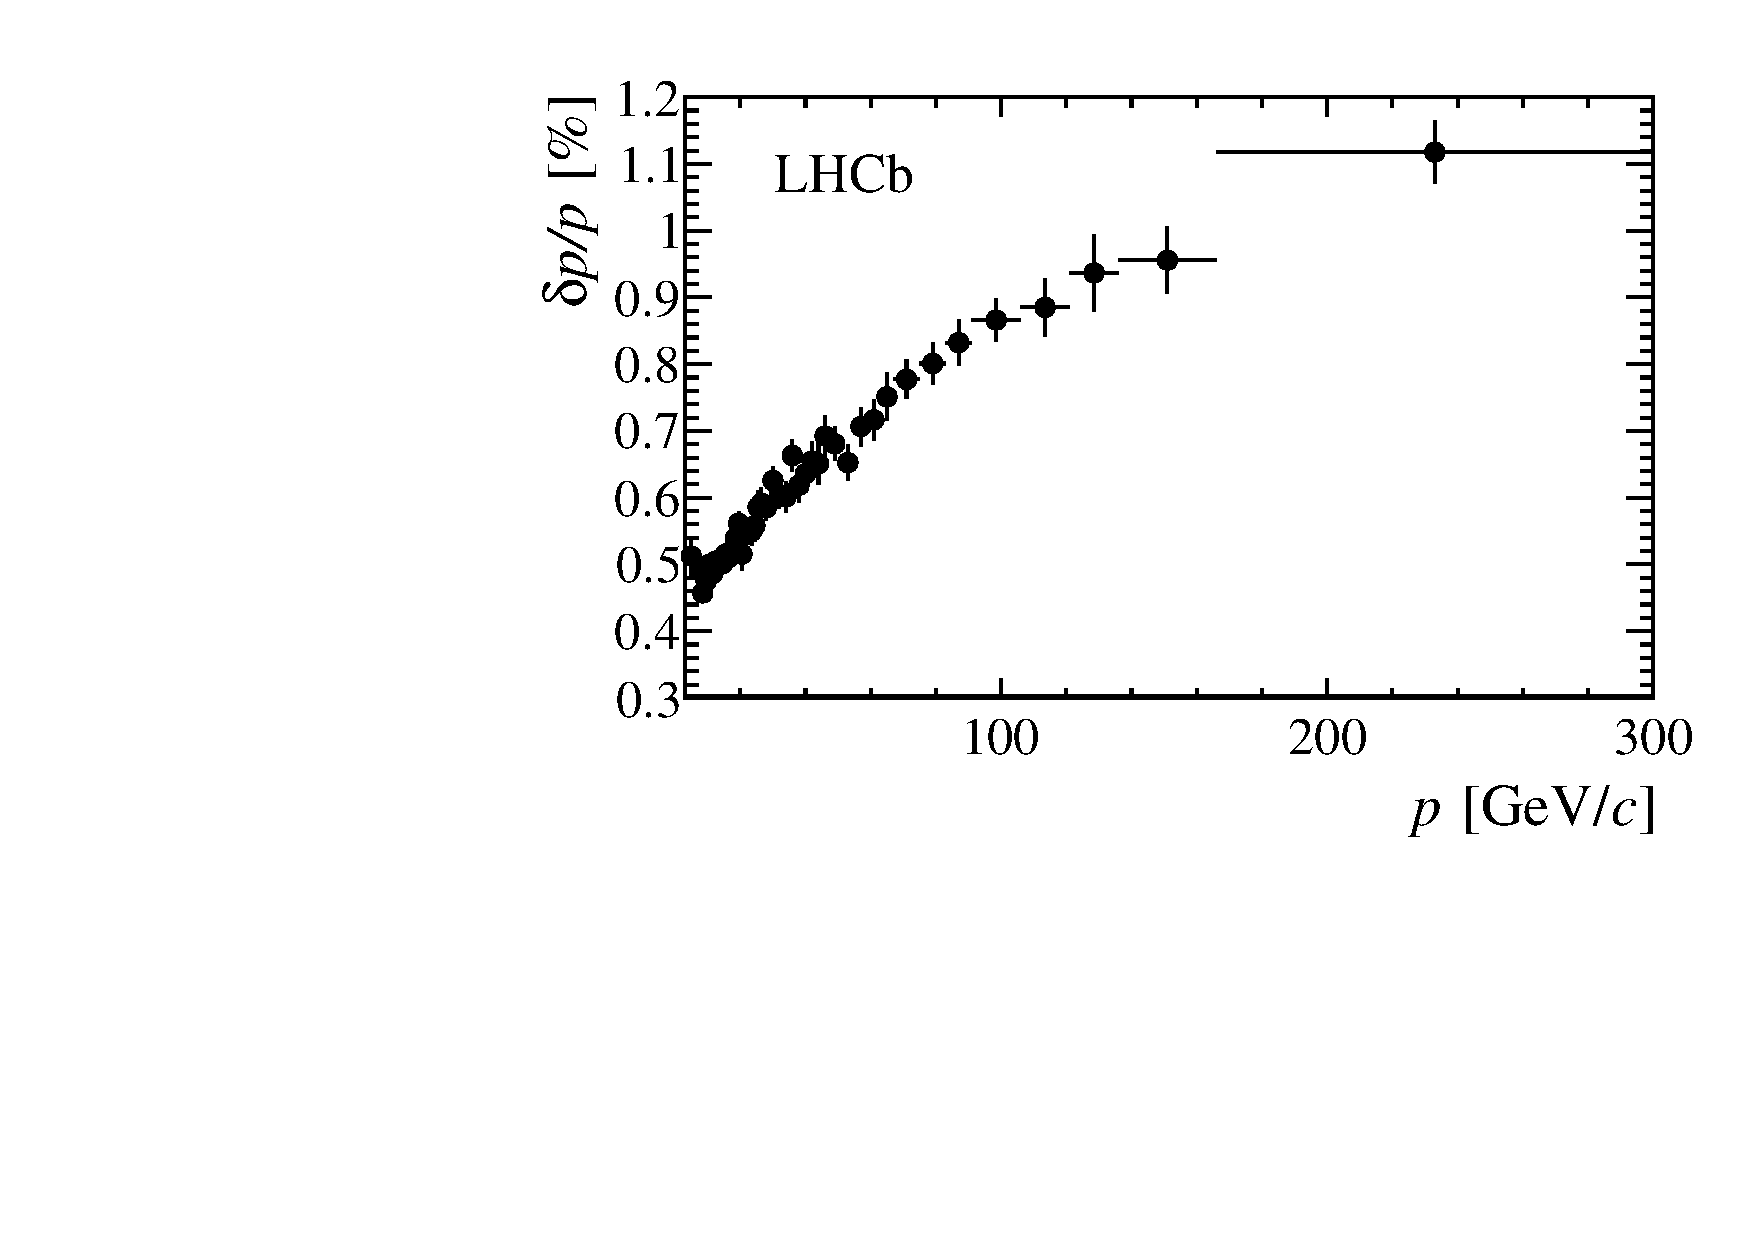
\includegraphics[width = 0.6\textwidth]{figs/detector/Fig17.pdf}
	\caption{Momentum resolution of \gls{longtrack}s measured at \gls{LHCb}. The decay channel $J/\psi \rightarrow \mu^{+} \mu^{-}$ is analysed for this purpose. Figure from \cite{LHCb-DP-2014-002}.}
	\label{fig:momres}
\end{figure}

\section{Ring Imaging \v{C}erenkov Detectors}
\label{richsec}
Particle identification, \Gls{PID}, at \Gls{LHCb} relies heavily on two dedicated Ring Imaging \v{C}erenkov subdetectors, \gls{RICH}. These detectors take advantage of the emission of \v{C}erenkov light, which happens when a charged particle travels through a medium at a speed faster than the phase velocity of light in that medium. This cone of light is emitted at an angle $\theta$ with respect to the charged particle's trajectory. Using the knowledge of refractive index of the medium, $n$, and momentum $p$ that is measured using the tracking system, the mass $m$ of the particle can be obtained through:

\begin{equation}
	\cos\theta_{c} =  \frac{\sqrt{m^{2} + p^{2}}}{pn}.
\end{equation}

As the momentum is not an intrinsic property of a passing particle, the momentum identification range is limited by the choice of medium, also known as radiator. For very low-momentum particle, as $\cos\theta_{c} \rightarrow 1$ ($p=\sqrt{\frac{m^{2}}{n^{2}-1}}$), the particle is not producing any \v{C}erenkov light cone. At the very high momentum, as $\cos\theta_{c} \rightarrow 1/n$, there is saturation point as all species of particles will emit the light at the same \v{C}erenkov angle, hence all the discriminating power will be lost.

Low momentum (2-60 \gev) particles are identified in the upstream \gls{RICH1} detector and high momentum particles (15-100) \gev are analyzed downstream in \gls{RICH2}. \gls{RICH1} covers angular acceptance of 25-300 mrad using $\rm{C_{4}F_{10}}$ ($n = 1.0014$) as radiator. \gls{RICH2} has more limited acceptance of 15-120 mrad and uses $\rm{CF_{4}}$ as radiator, with lower $n=1.0005$. The discrimination power between different particles can be seen in~\autoref{fig:richres}(a). 


Both \gls{RICH1} and \gls{RICH2} use a set of spherical primary mirrors to guide the photons onto the flat secondary mirrors which are then further focused into \v{C}erenkov rings on the surface of a plane of Hybrid Photon Multipliers, (\Gls{HPD}). The schematic view of a particle passing through \gls{RICH1} can be seen in~\autoref{fig:richres}(b). 


\begin{figure}[!h]
	\centering
	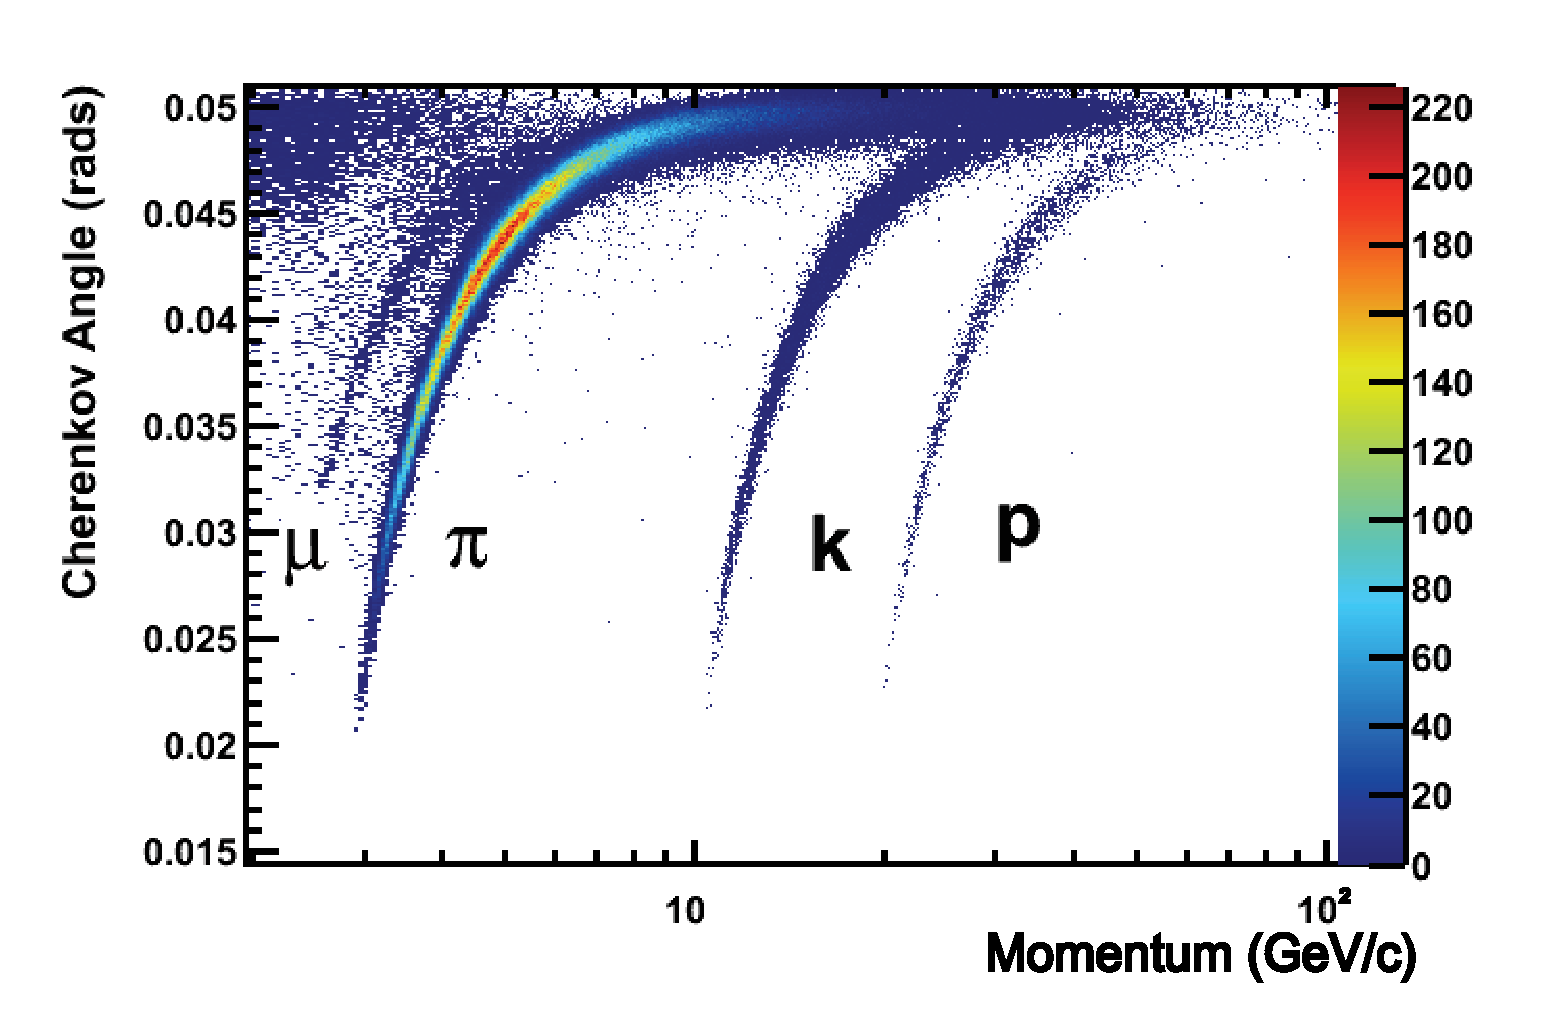
\includegraphics[width = 0.5\textwidth]{figs/detector/CKAnglevsMom_NoTheory_jun2011-01.eps}\put(-50,170){(a)}%
	%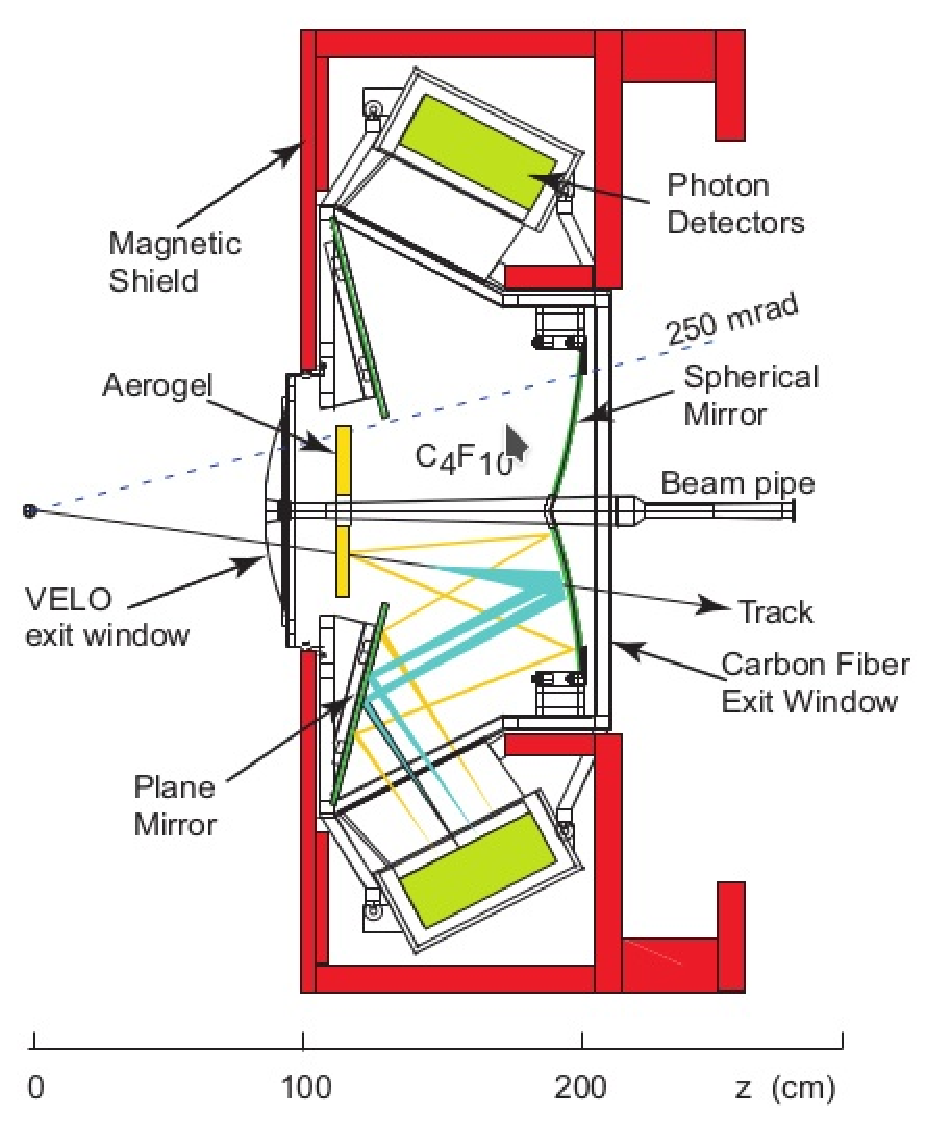
\includegraphics[width = 0.4\textwidth]{figs/detector/mechrich.eps}%
	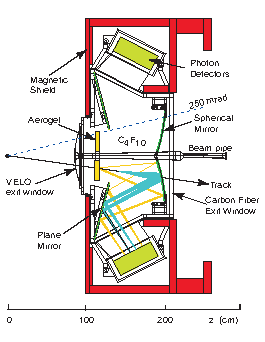
\includegraphics[width = 0.4\textwidth]{figs/detector/license/Rich_croped.pdf}\put(-10,170){(b)}%
	\caption{ (a) Separation power for different species of particles in momentum-\v{C}erenkov angle plane for $\rm{C_{4}F_{10}}$ radiator. Figure from \cite{LHCb-DP-2012-003}. (b) Schematic diagram of \gls{RICH1} layout. Figure from \cite{det_paper}.}
	\label{fig:richres}
\end{figure}

\section{RICH Reconstruction and Performance }
In order to establish species of particles for each track, the \v{C}erenkov angle is combined with the track momentum measured by tracking. In practice, however, as \Gls{RICH} detectors operate in high track density environment, many \v{C}erenkov rings will be overlapping and hence a complex pattern recognition algorithm is deployed \cite{Forty:1999sg}. 


For each event, the \Gls{RICH} computes a full event likelihood that is consistent with assigning a pion mass hypothesis to all tracks given the observed hit distribution read out by the \Gls{HPD}s. The algorithm then iterates through all other possible particle species, ($e, \mu, \pi, K,$ proton, deuteron), assigning a new full event likelihood for a given track, having all other hypotheses fixed. The mass hypothesis with the highest full event likelihood is assigned to the track and this process is repeated for all the tracks in the event, until no improvement is found. 

Results of this algorithm provide likelihood variables, $\rm{\textrm{DLL{x}}}$, that quantify the strength of the chosen species hypothesis against the pion hypothesis,
\begin{equation}
	\textrm{\textrm{DLL{x}}} = \mathrm{log}(\mathcal{L})_{x} - \mathrm{log}(\mathcal{L})_{\pi} \quad  x\in{e, \mu, K, \rm{proton, deuteron}}.
\end{equation}

By calculating $\rm{DLL{x_{1}} - DLL{x_{2}}}$, one can obtain discriminative strength between any two species.

\subsection{RICH Performance}
\label{RICHperf}
In order to measure the performance of the \Gls{PID} computed by a \gls{RICH}, populous calibration samples with very little background contamination are required. In order not to bias results, these samples have no \Gls{PID} constraints themselves and are reconstructed solely using kinematic information. For studies of pion/kaon efficiencies, $D^{*+} \to D^{0}(\kaon^{-}\pip)\pip$ backround-substracted samples are used, whereby the daughter tracks of $D^{0}$ become proxies for the evaluation. The invariant mass for the $D^{0}$ candidates can be seen in~\autoref{fig:richperf}(a) The probability of correctly identifying a kaon given a certain constraint on $\textrm{DLL{K}}$, identification efficiency (\Gls{ID}), and probability of mistakenly swapping pion identification, misidentification efficiency (\gls{misID}), are summarized in~\autoref{fig:richperf}(b). Identification probabilities of $\approx$ 85\% with misID rate of $\approx$ 3\% provide invaluable discriminating separation between kaons and pions.




\begin{figure}[!h]
	\centering
	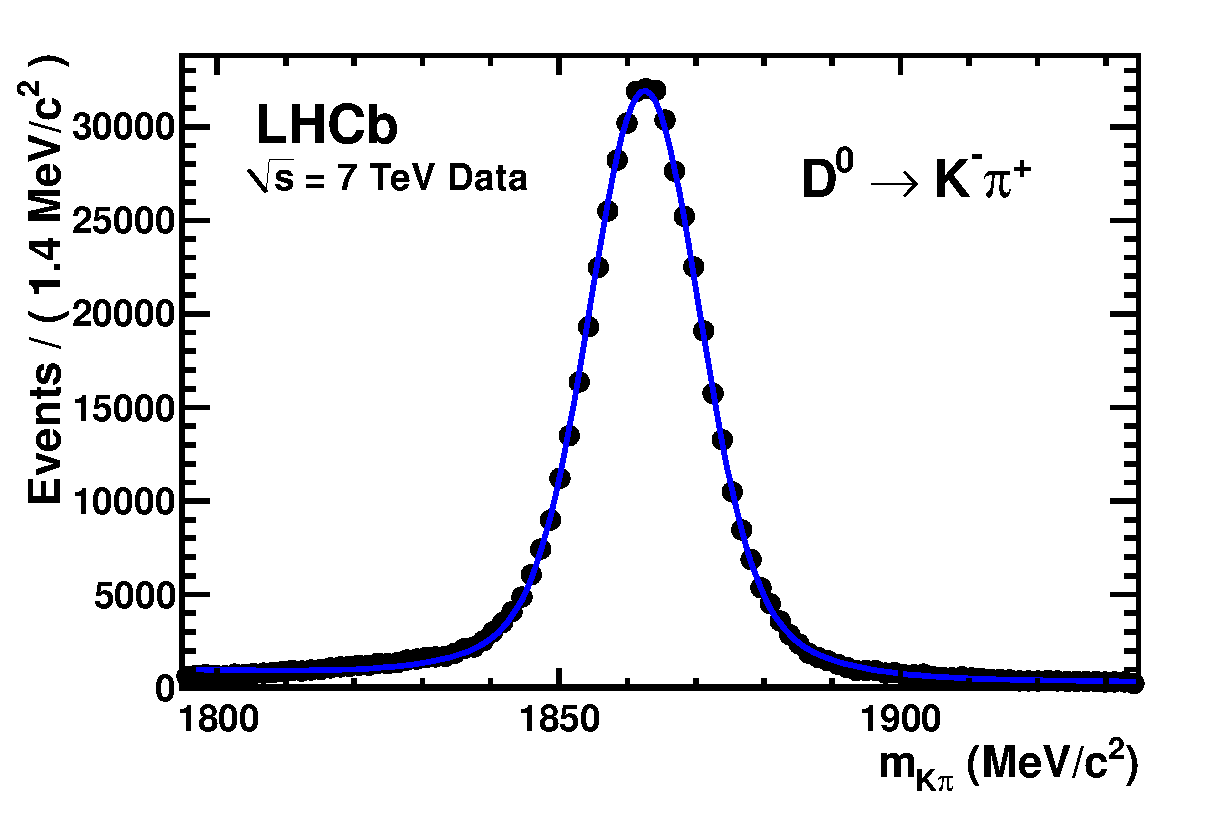
\includegraphics[width = 0.525\textwidth]{figs/detector/D0_Mass.eps}\put(-50,80){(a)}%
	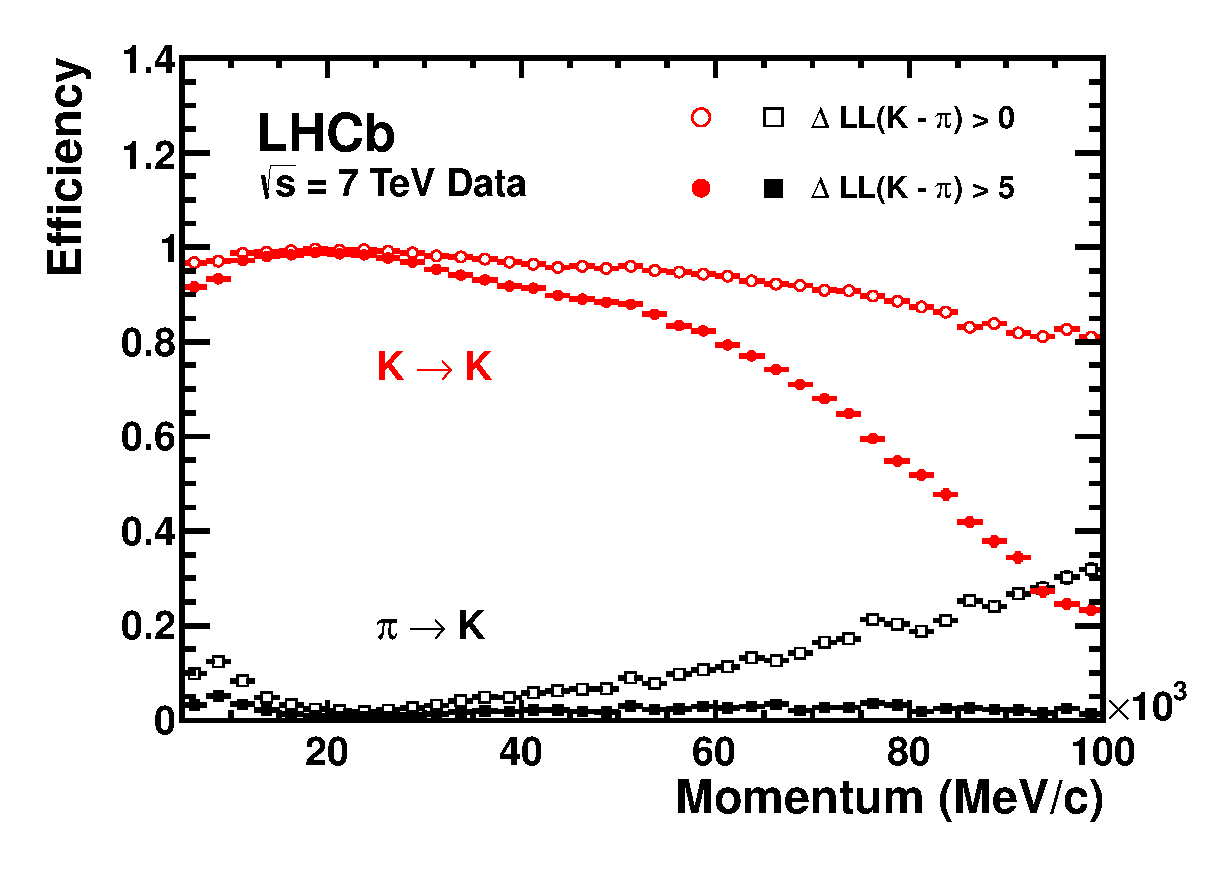
\includegraphics[width = 0.5\textwidth]{figs/detector/KandPi_2_K.eps}\put(-50,80){(b)}%
	\caption{ (a) Invariant mass distribution of $D^{0}$ data sample (in black) overlaid with fit to both background and signal (in blue). (b) An example of kaon ID (red) and misID (black) efficiency as a function of momentum under two \gls{PID} hypotheses, $\textrm{DLL{K}} > 0$ (empty)  and $\textrm{DLL{K}} > 5$ (filled). Both Figures from \cite{LHCb-DP-2012-003}.}
	\label{fig:richperf}
\end{figure}

%In search for $B^{0}$ and $B^{0}_{s}$ decaying to $h^{+}h^{-}$, where $h\in K, \pi$, $\pi^{+} \pi^{-}$ invariant mass spectra with and without \gls{PID} $\textrm{DLL{x}}$ requirements can be seen in~\autoref{fig:richnice}. These plots clearly demonstrate increase in sensitivity searching for $B^{0} \rightarrow \pi^{+} \pi^{-}$ signal amongst other components. 

%\begin{figure}[!h]
%	\centering
%	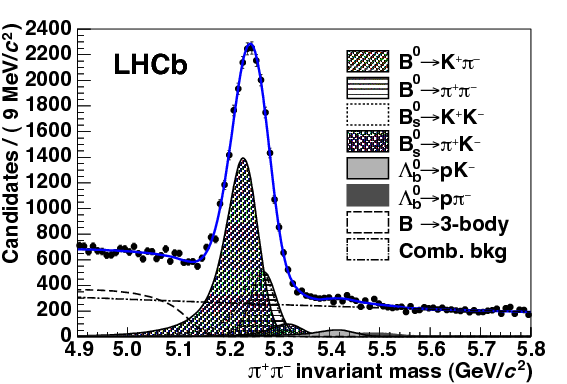
\includegraphics[width = 0.5\textwidth]{figs/detector/b2hhnopid.png}%
%	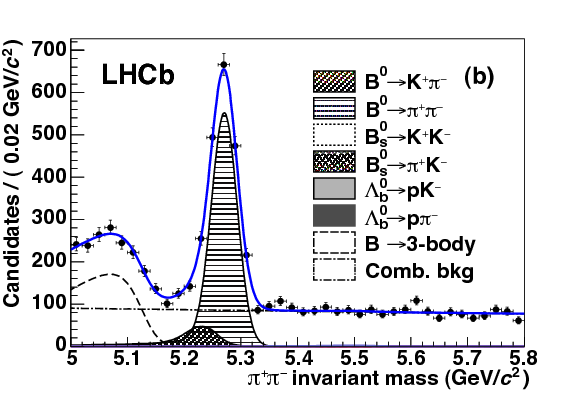
\includegraphics[width = 0.5\textwidth]{figs/detector/b2hhpid.png}%
%	\caption{ $\pi^{+} \pi^{-}$ invariant mass distributions obtained using kinematic constraints only (left) and also using \gls{PID} constraints (right) in order to isolate $B^{0} \rightarrow \pi^{+} \pi^{-}$ peak. This figure is taken from \cite{LHCb-PAPER-2012-002}. }  
%	\label{fig:richnice}
%\end{figure}


\section{Calorimetry }
\label{calosys}
As many other particle physics detectors, \Gls{LHCb} is equipped with series of subdetectors providing separation between electrons, pions and photons. This separation is achieved because different particles interact differently with the material, producing differently shaped showers. This part of the detector is not only integral to the way the \Gls{LHCb} trigger system works but it also provides a measurement of energies of these objects.
All the subcomponents discussed here operate on the same principle. Passing particles through the material emit light. The light from the scintillating material, which is created by absorbing the energy of the passing particle and re-emitted it in form of light, is guided to photomultiplier tubes by wavelength shifting fibres.

Electrons, pions and photons firstly encounter two planes of scintillating tiles: the Scintillating Pad Detector (\Gls{SPD}), and the Preshower Detector (\Gls{PRS}) intersected by a wall of lead. The \Gls{SPD} senses the passage of charged particles as they emit light whereas neutral particles do not, making this subdetector distinguish between electrons and photons. The wall of lead initiates the electromagnetic shower, where photons are converted into electron-positron pairs, depositing sizable energy in the \Gls{PRS} allowing electron/pion separation. 

The Electromagnetic Calorimeter (\Gls{ECAL}) in \gls{LHCb} is based on a sampling shashlik-type technology, where scintillating tiles are alternated by lead plates measuring the energy deposit of electromagnetic showers. As the best energy resolution requires full energy deposit of energetic photons along the \Gls{ECAL}, the thickness is equivalent to 25 radiation lengths. The resulting resolution of the \Gls{ECAL} is $\frac{\sigma_{E}}{E} = \frac{10\%}{\sqrt{E}} \oplus 1\%$, where $E$ is in \gev.

On the other hand, the Hadronic Calorimeter \Gls{HCAL} sandwiches iron instead of lead as the absorber with thickness of 5.6 interaction length only, achieving a resolution of $\frac{\sigma_{E}}{E} = \frac{70\%}{\sqrt{E}} \oplus 10\%$ in beam tests. This poorer resolution however fulfils the requirements necessary for the main purpose of this detector, which is the hadron trigger. Away from the beampipe the granularity of cells is coarser to mirror the track occupancy as seen in~\autoref{fig:CaloGran}(a)(b). 

\begin{figure}[!h]
	\centering
	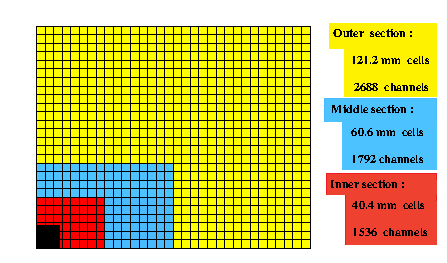
\includegraphics[width = 0.5\textwidth]{figs/detector/license/ECAL_crop.pdf}\put(-70,10){(a)}%%
	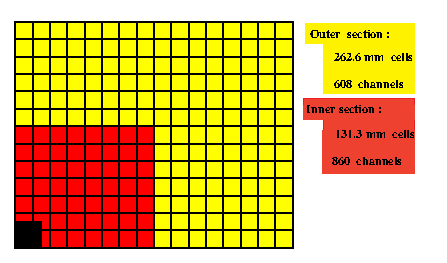
\includegraphics[width = 0.5\textwidth]{figs/detector/license/HCAL_crop.pdf}\put(-70,10){(b)}%%
	\caption{Granularity of (a) \Gls{ECAL} and (b) \Gls{HCAL} detectors. This is just a quarter view and that the black region is where the beam pipe is located. Figure from \cite{det_paper}. }  
	\label{fig:CaloGran}
\end{figure}




\section{Muon Stations }
\label{muonsys}
Muons are considered to be of fundamental importance to many flagship analyses by \Gls{LHCb}, such as the search for the rare $\B^{0}_{s} \rightarrow \mu^{+} \mu^{-}$ decay\cite{Aaij:2017vad}. Analysis of \Bmumumu of course relies heavily on good performance of this part of detector. Muon stations are positioned at the end of the detector, taking advantage of the fact that muons penetrate material better than any other particle type. 

\Gls{LHCb}'s five rectangular muon stations \Gls{muonstation} are positioned before and after calorimetry system, with first station M1 upstream of the \Gls{SPD}, and four stations (M2-M5) downstream of \Gls{HCAL} as shown in~\autoref{fig:MuonGran}. The M1 station consists of 12 sets of three gas electron 
multiplier foils (triple-GEMs) in the region closest to the beam pipe, resisting the highest dose of radiation due to the highest particle flux. Its main use lies in improving the measurement of $p_{T}$ in the hardware trigger. The M2-M5 stations each consist of 276 multi-wire proportional chambers (\Gls{MWPCs}) filled with an $\rm{Ar,CO_{2},CF_{4}}$ gas mixture. They are interlayered with 0.8\m iron walls, to provide a stopping target for all particles, other than muons with momentum higher than $6$ \gevc.

%In order to ease the accessibility, like in \Gls{VELO}, all the stations are split into two independent mechanical sides, also known A and C side.

Each half of a muon station is segmented into four increasingly larger regions away from the beam, R1 to R4.
 All the regions were constructed to cover the same acceptance, keeping the track occupancy constant across the station. The granularity of the readout is higher in the horizontal plane to take advantage of the magnet's horizontal bending plane.




\begin{figure}[!h]
	\centering
	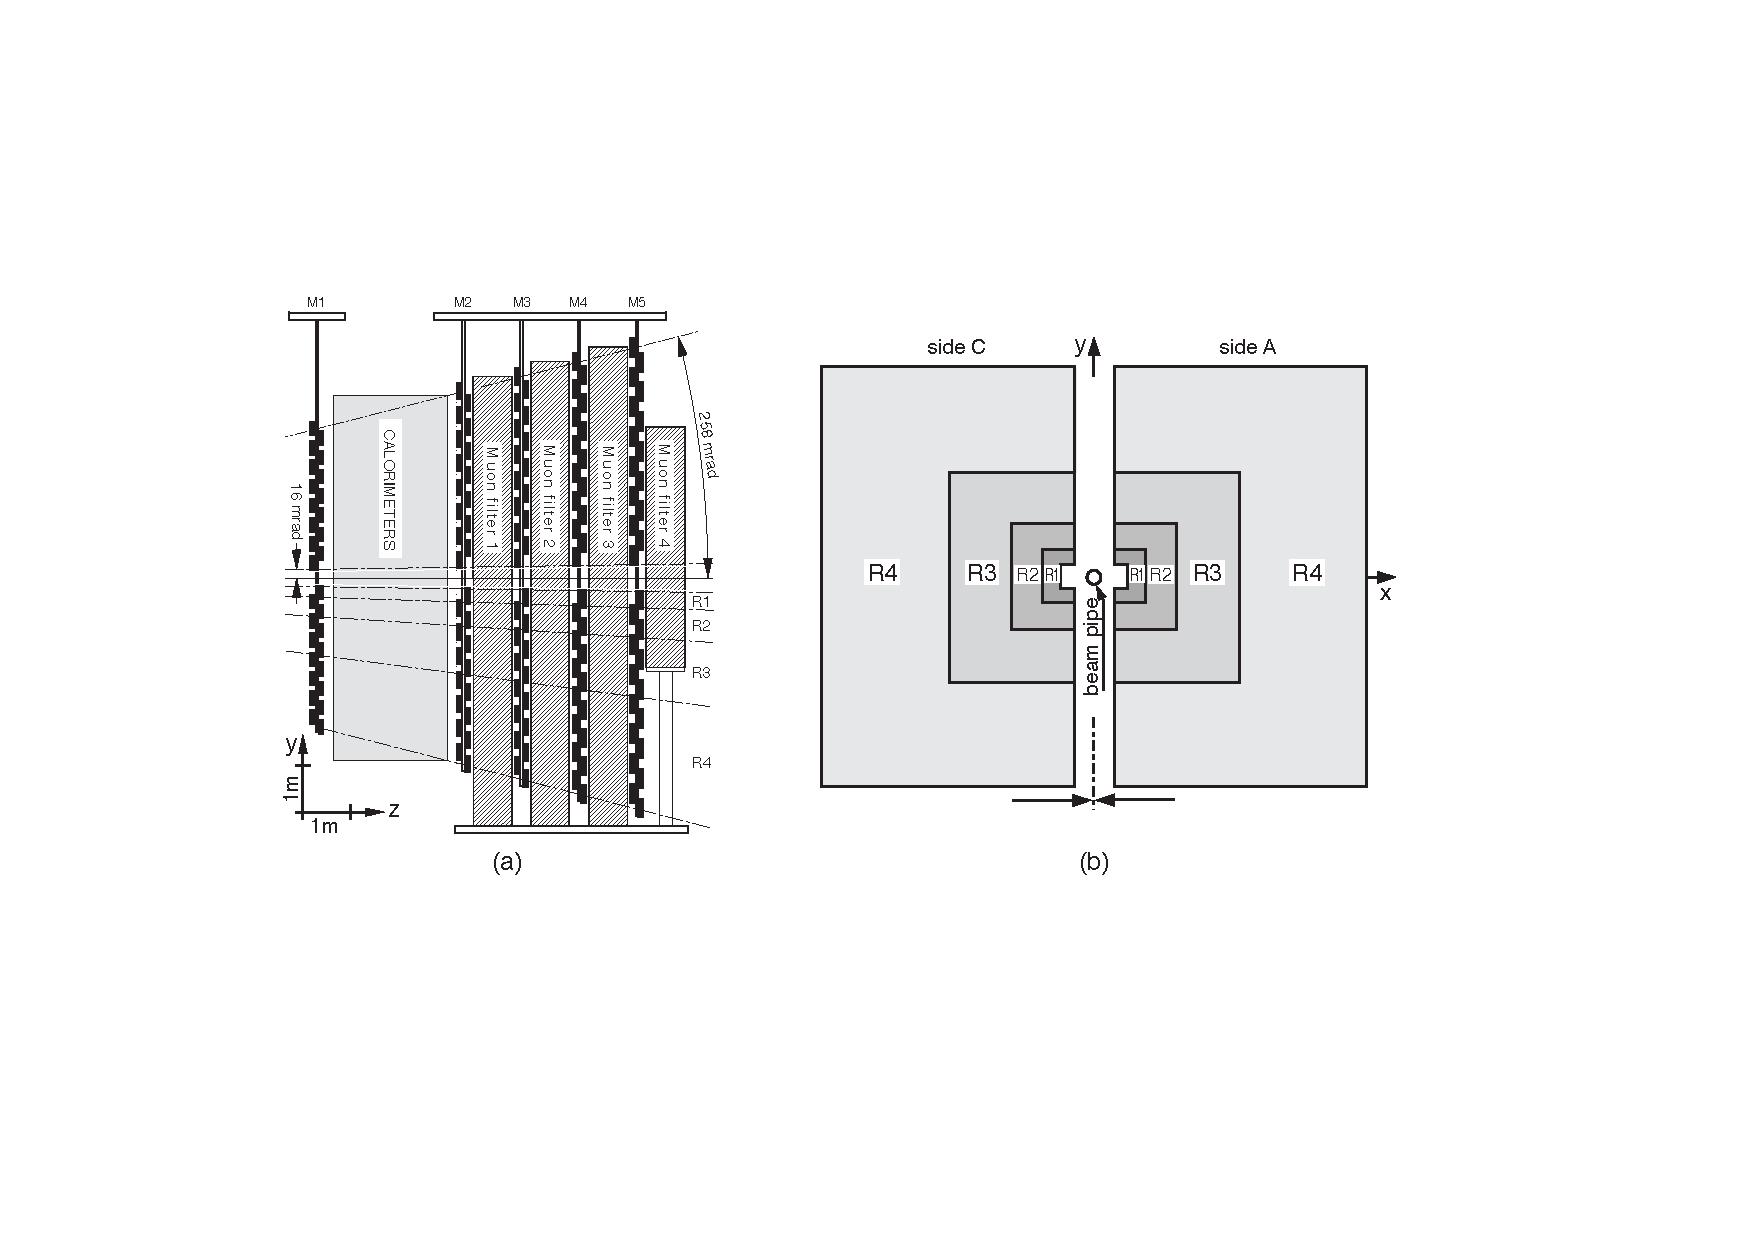
\includegraphics[width = 1.0\textwidth]{figs/detector/sideview.pdf}%
	%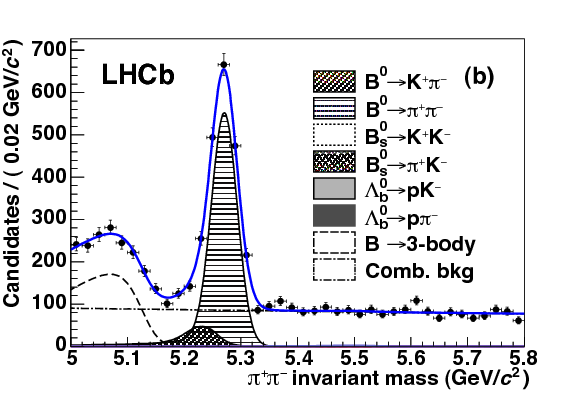
\includegraphics[width = 0.5\textwidth]{figs/detector/b2hhpid.png}%
	\caption{(a) Layout of the muon detector x-z plane and (b) x-y plane. Figure from \cite{LHCb-DP-2012-002}. }  
	\label{fig:MuonGran}
\end{figure}

Both GEM and \Gls{MWPCs} operate on a same principle. In each station, the position in the $x-y$ plane is determined by ionizing electrons that come from muons passing through the detector, which are then attracted either to the closest anode mesh or wire mesh. The trigger is fired if the corresponding rectangular region in each station registered a positive binary decision. This means an efficiency of each station must be $\geq$99\% to give overall 95\% trigger efficiency. %Geometrical layout covers $\approx$ 20\% muons originating in semileptonic $b$ decays.\mybox{\color{red}CERN-THESIS-2012-025.pdf from puig, i have to invedtigate}


\subsection{Muon Identification }
\label{muonID}
Apart from triggering events with high enough $p_{T}$ muons, the muon stations provide necessary \gls{PID} information for muon analyses. Offline variables mostly used for muon ID by analysts are
\begin{itemize}
	\item{\textbf{IsMuon}: Boolean decision of muon candidates with momentum-dependent categorisation. Long tracks with $p>3$\gev/c are extrapolated to muon stations yielding $x-y$ coordinates in M2-M5, considering only tracks within acceptance. For each station, a search for hit information within an elliptical area defined by momentum, a field of interest (\Gls{FOI}), is performed. The hit requirements are summarized in~\autoref{tab:ismuontab}.}
	\item{\textbf{muDLL}: Difference in log likelihoods computed using muon and non-muon hypothesis. These hypotheses are based on the proximity/distance $D^{2}$ of the track extrapolation into the muon stations and corresponding closest sensed hits in those stations. Muon-like particle will tend to have sharper distribution in $D^{2}$ as compared to other species. Protons were chosen to be the other species for the calibration purposes. They give a broader distribution as they originate either as punch-through protons (protons coming from showers not fully contained in the \gls{HCAL}), protons having coincident hit position to a true muon, or random hits.}
	\item{\textbf{DLLmu}}:  For each track a global likelihood is produced, by combination of muon and non-muon likelihood from \textbf{muDLL}, with the \Gls{RICH} different mass hypothesis likelihoods, and calorimetry likelihood exploiting the energy deposits information. Like in the \Gls{RICH} likelihoods, the default hypothesis corresponds to separation between the muon and pion hypotheses.    

\end{itemize}

\noindent Other variables which are extensively used for muon particle identification in search for \Bmumumu are described in~\autoref{otherpid}. 

\begin{table}[!h]
	\centering
	\hspace*{-0.8cm}
	\begin{tabular}{c c}
		\toprule
		Particle Momentum $p$  & Hits in Muon Stations \\ \hline
		3 \gev/c <$p$<6 \gev/c & M1 $\&$ M2\\
		6 \gev/c <$p$<10 \gev/c & M1 $\&$ M2 $\&$ (M3 $||$ M4) \\
		10 \gev/c <$p$ & M1, M2, M3 and M4 \\ \bottomrule      
	\end{tabular}
	\caption{Momentum-dependent definition \texttt{IsMuon} variable.}
	\label{tab:ismuontab}
\end{table}   

\subsection{Muon Identification Performance}
\label{muonperf}
As for hadron performance measurements, the muon ID performance is determined using the high statistics decay channel $J/\psi \rightarrow \mu^{+} \mu^{-}$ with a \textit{tag and probe} method. MisID rates of kaons and pions are computed using the same decay channels, which were used for identification of hadrons, $D^{*+} \to D^{0}(\kaon^{-}\pip)\pip$. The summary of \texttt{IsMuon} ID and misID rates are presented in~\autoref{fig:MuonID}. Very high ID rate (above 90\%) for relatively low misID probability (below 10\%) is key to analyses with muons in a final state. But the least performing are the low $p_{T}$ muons where the identification suffers because these muons can end up outside of the \gls{LHCb} acceptance and misID rates for kaon and pions are significantly higher in low momenta region as the dominant process causing this are muons from decay-in-flight.   

\begin{figure}[!h]
	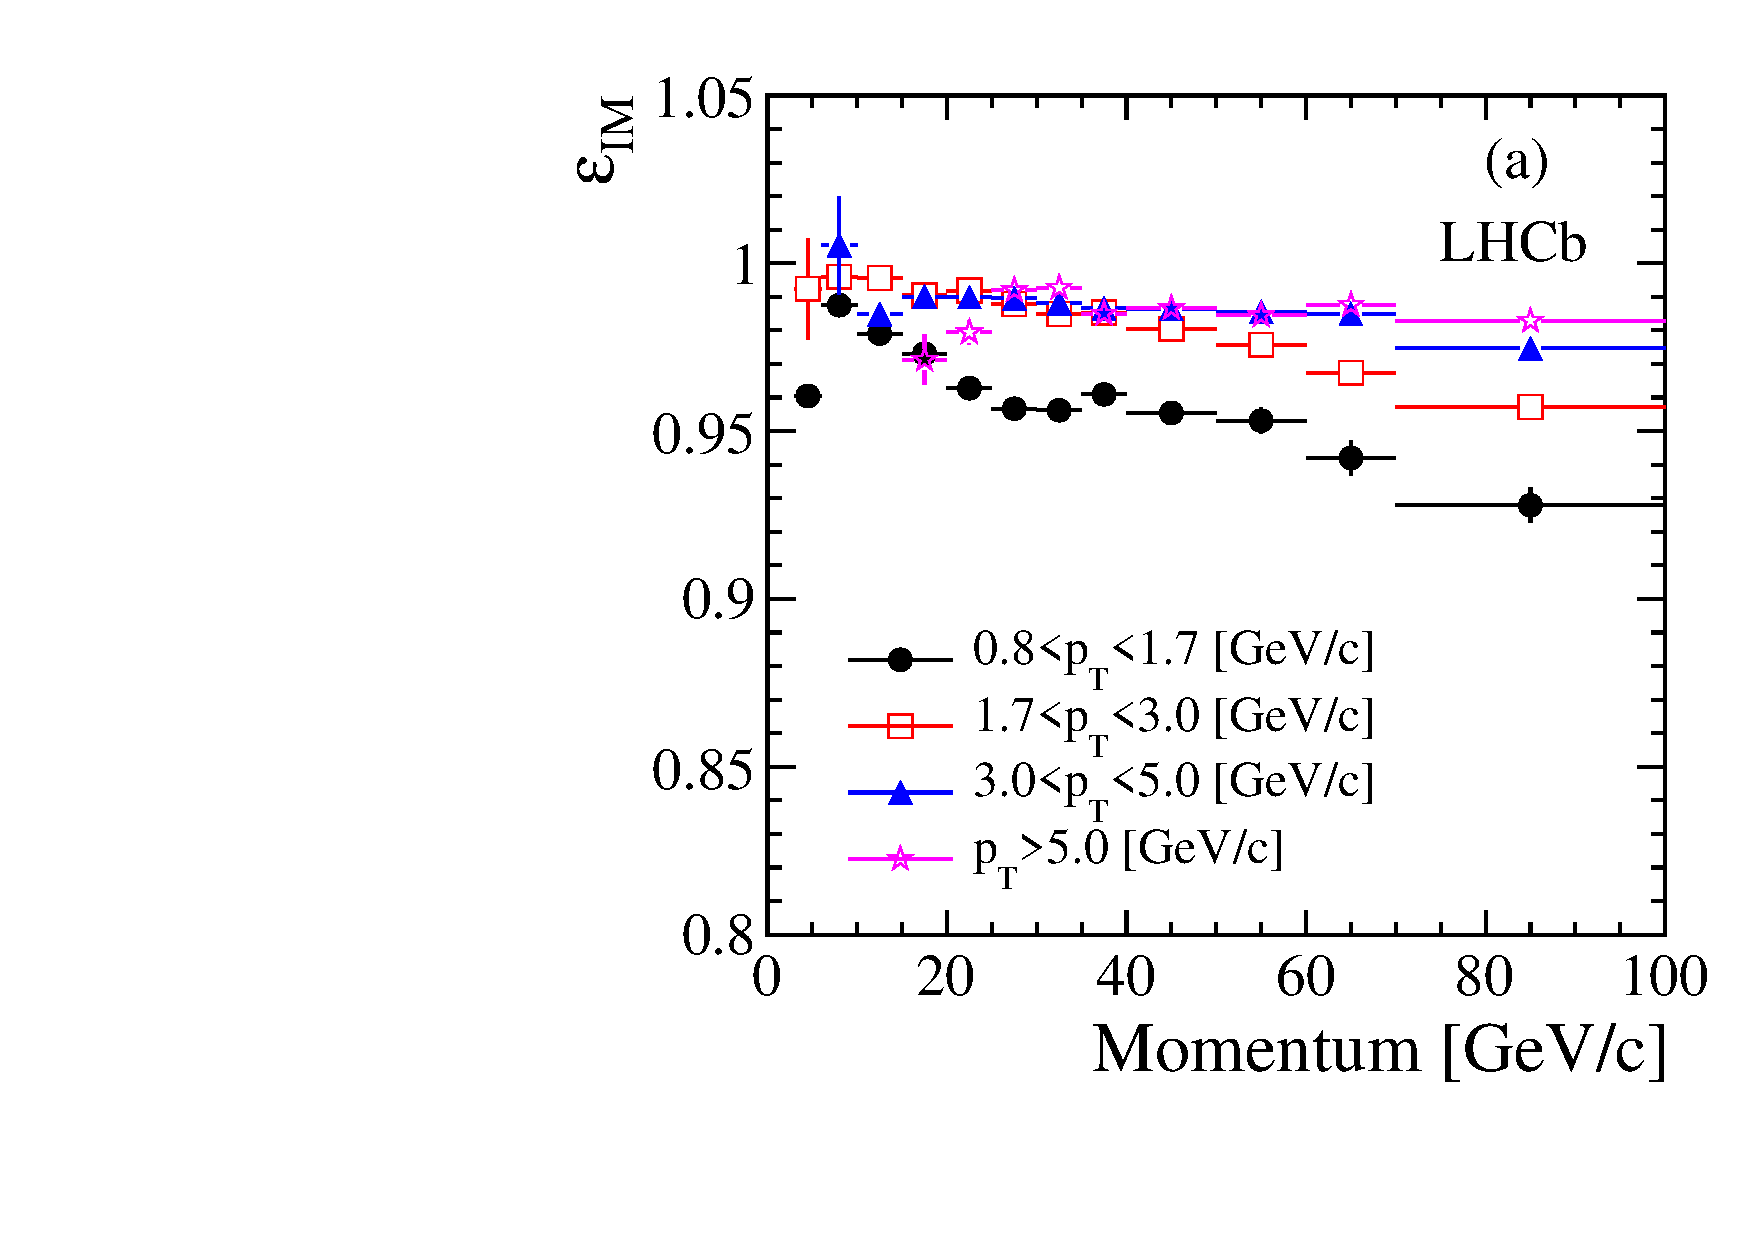
\includegraphics[width = 0.5\textwidth]{figs/detector/dllFit_mu_IMvsPvsPt.pdf}%
	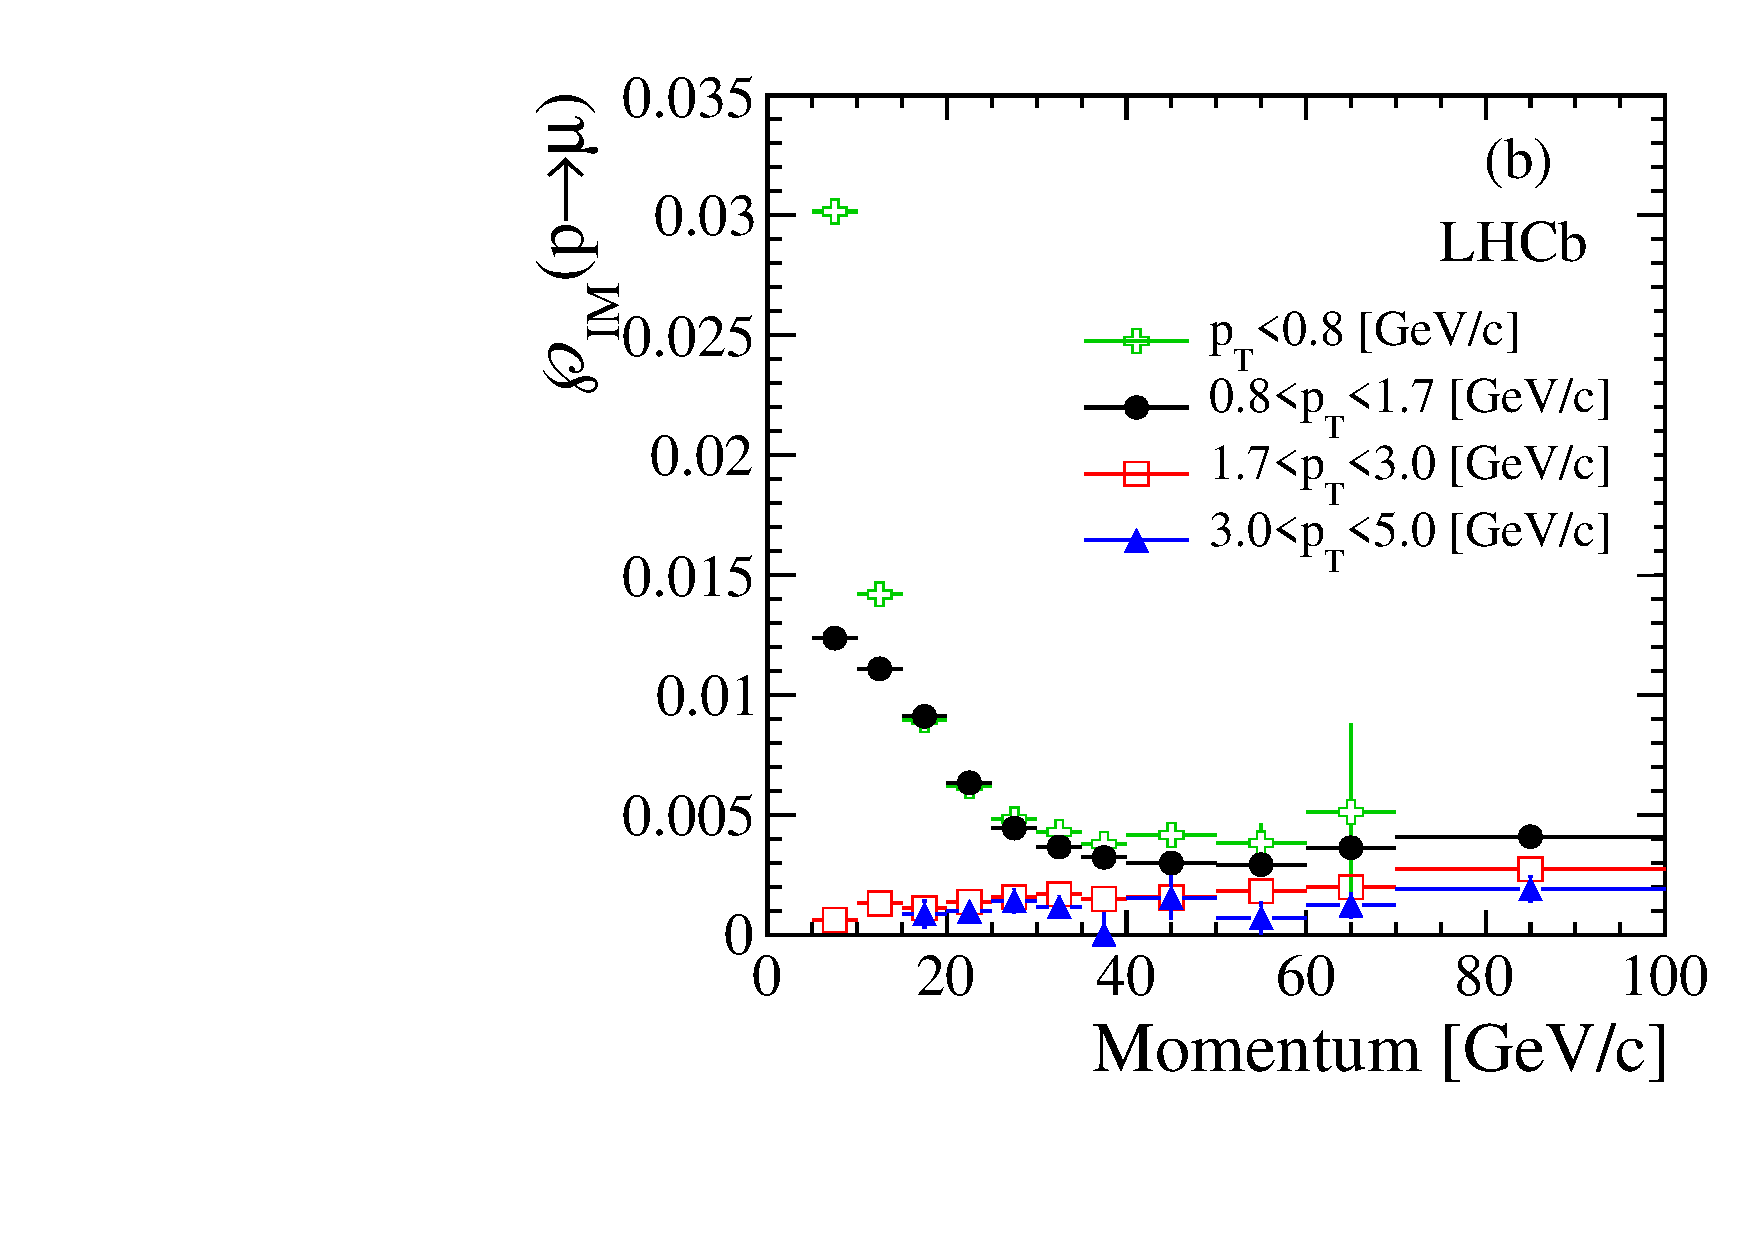
\includegraphics[width = 0.5\textwidth]{figs/detector/dllFit_P_IMvsPvsPt.pdf}%
       \newline
	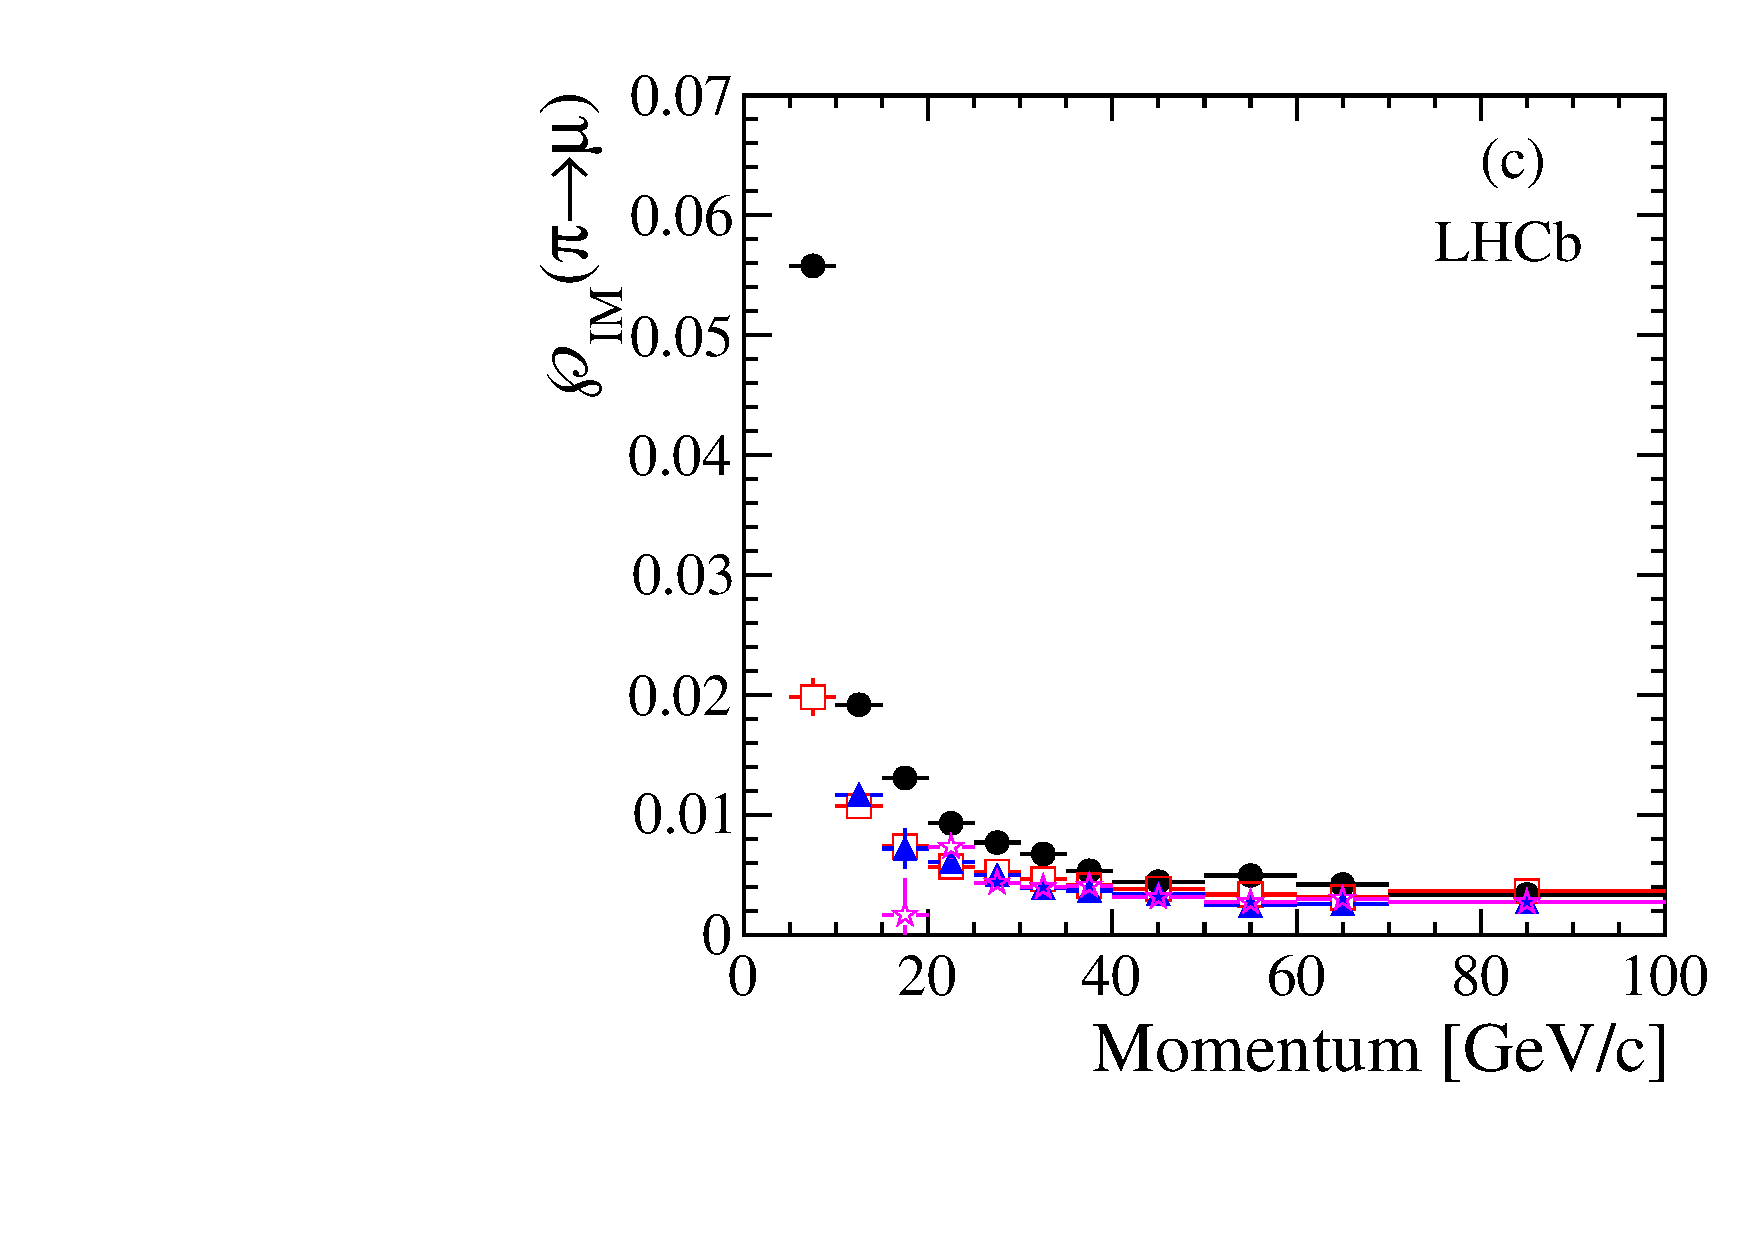
\includegraphics[width = 0.5\textwidth]{figs/detector/dllFit_pi_IMvsPvsPt.pdf}%
	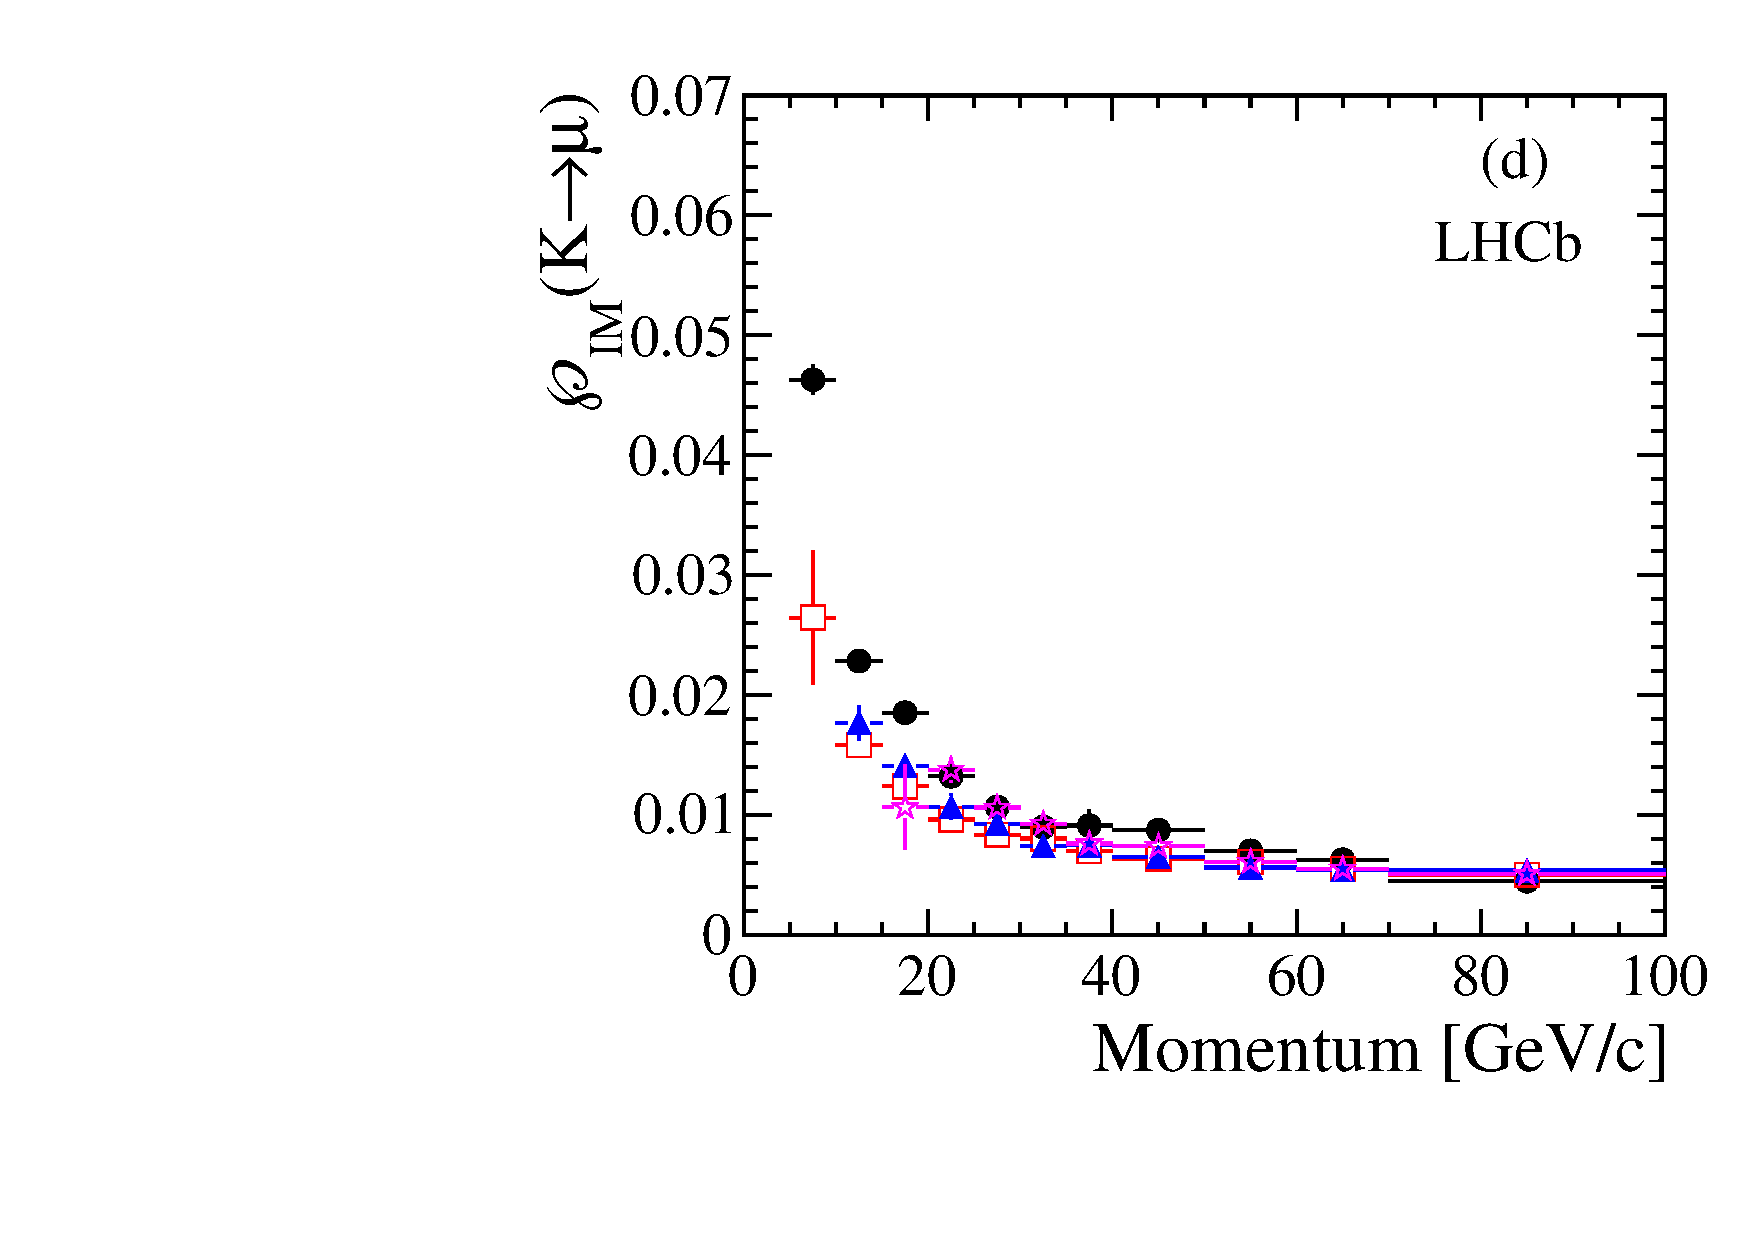
\includegraphics[width = 0.5\textwidth]{figs/detector/dllFit_ka_IMvsPvsPt.pdf}%
	\caption{(a) Probability of correctly identifying muons as a function of momentum $p$ in the bins of $p_{T}$ for $J/\psi \rightarrow \mu^{+} \mu^{-}$ with \texttt{IsMuon} constraint. (c) Probability of incorrectly identifying pion (b) proton and (d) kaon as muon with \texttt{IsMuon}. This figure is taken from \cite{LHCb-DP-2013-001}. }  
	\label{fig:MuonID}
\end{figure}


\section{Trigger }
\label{triggerchap}
Big-data physics experiments have to make decisions on what kind of data they want to keep. The choice of interesting events is performed by a series of decisions, which is known as the trigger. The \Gls{LHCb} trigger system was build around constraints posed by the run conditions, read-out capabilities and available disk space. In Run \Rn{1} and Run \Rn{2} \gls{LHCb} has at its disposal the multistage trigger consisting of a hardware-based level 0 trigger (\Gls{L0}) and a software-based high level trigger (\Gls{HLT}).

In the end, selected events have their trigger decisions categorized. An event where the signal candidate caused the trigger to fire is known to be Trigger on Signal (\Gls{TOS}). An event where it is a non-signal like particle causing the trigger decision to occur, Trigger Independent of Signal (\Gls{TIS}) is labelled. Finally, if only by a combination of signal particle(s) together with other particle's properties in the event produce an affirmative decision, then these events are categorized as \Gls{TIS} $\&$ \Gls{TOS} = \Gls{TISTOS}.

\Gls{L0} reduces the rate of data from 40 \mhz to 1 \mhz by employing five trigger decisions, also known as lines. The first three lines make decision using calorimeter information about the transverse energy, $E_{T}$, whether it is photon, electron or hadron causing the shower energy deposit. Two other lines are reading out information from the muon system by looking for transverse momentum, $p_{T}$, of muon and dimuon (two muon tracks) objects. Efficiencies of the L0 muon triggers are evaluated using $B^{+} \rightarrow (J/\psi \rightarrow \mu^{+} \mu^{-}) K^{+}$ decays and can be seen in~\autoref{fig:L0Perf}(a). The hadron trigger efficiency in different decay channels can be seen in~\autoref{fig:L0Perf}(b). 


\begin{figure}[!h]
	\centering
	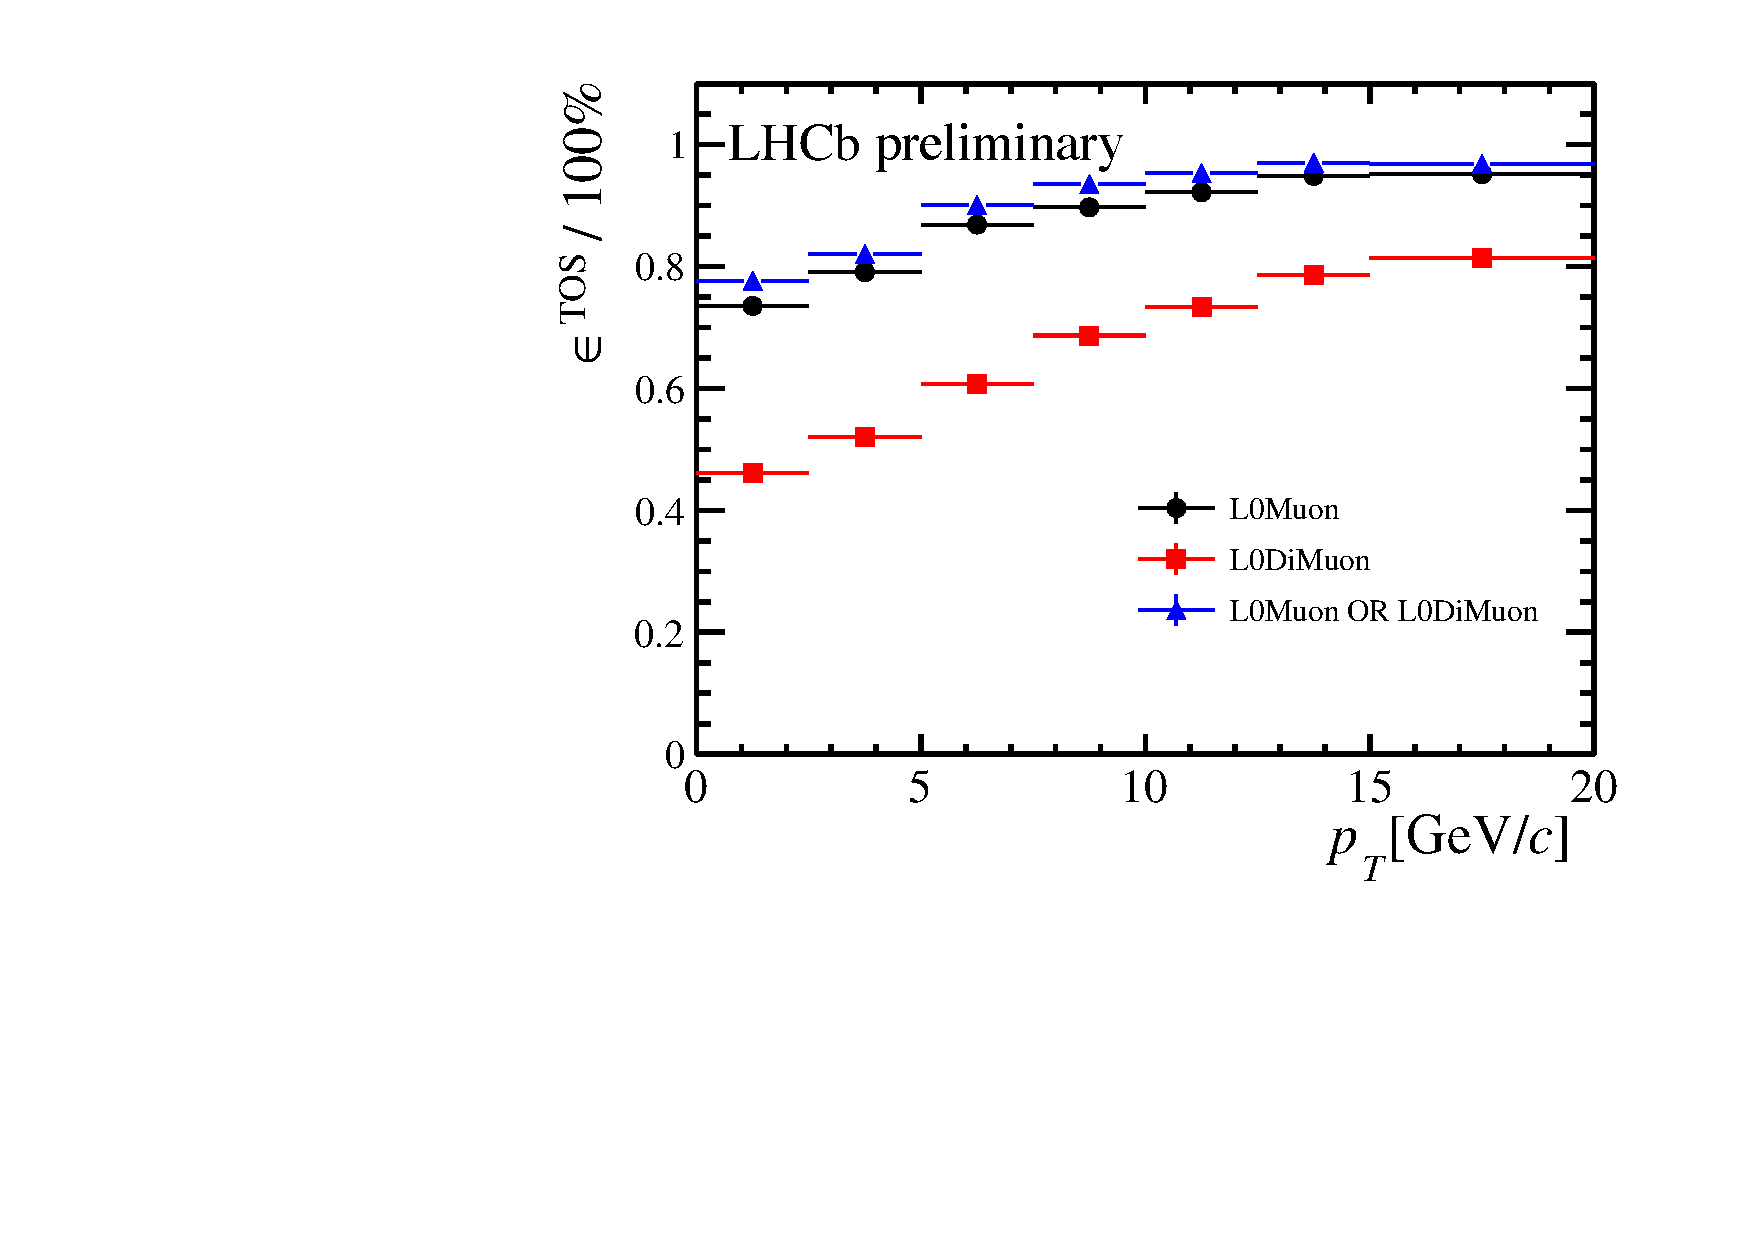
\includegraphics[width = 0.5\textwidth]{figs/detector/Fig1_L0MuonEff_PT.pdf}\put(-50,90){(a)}%
	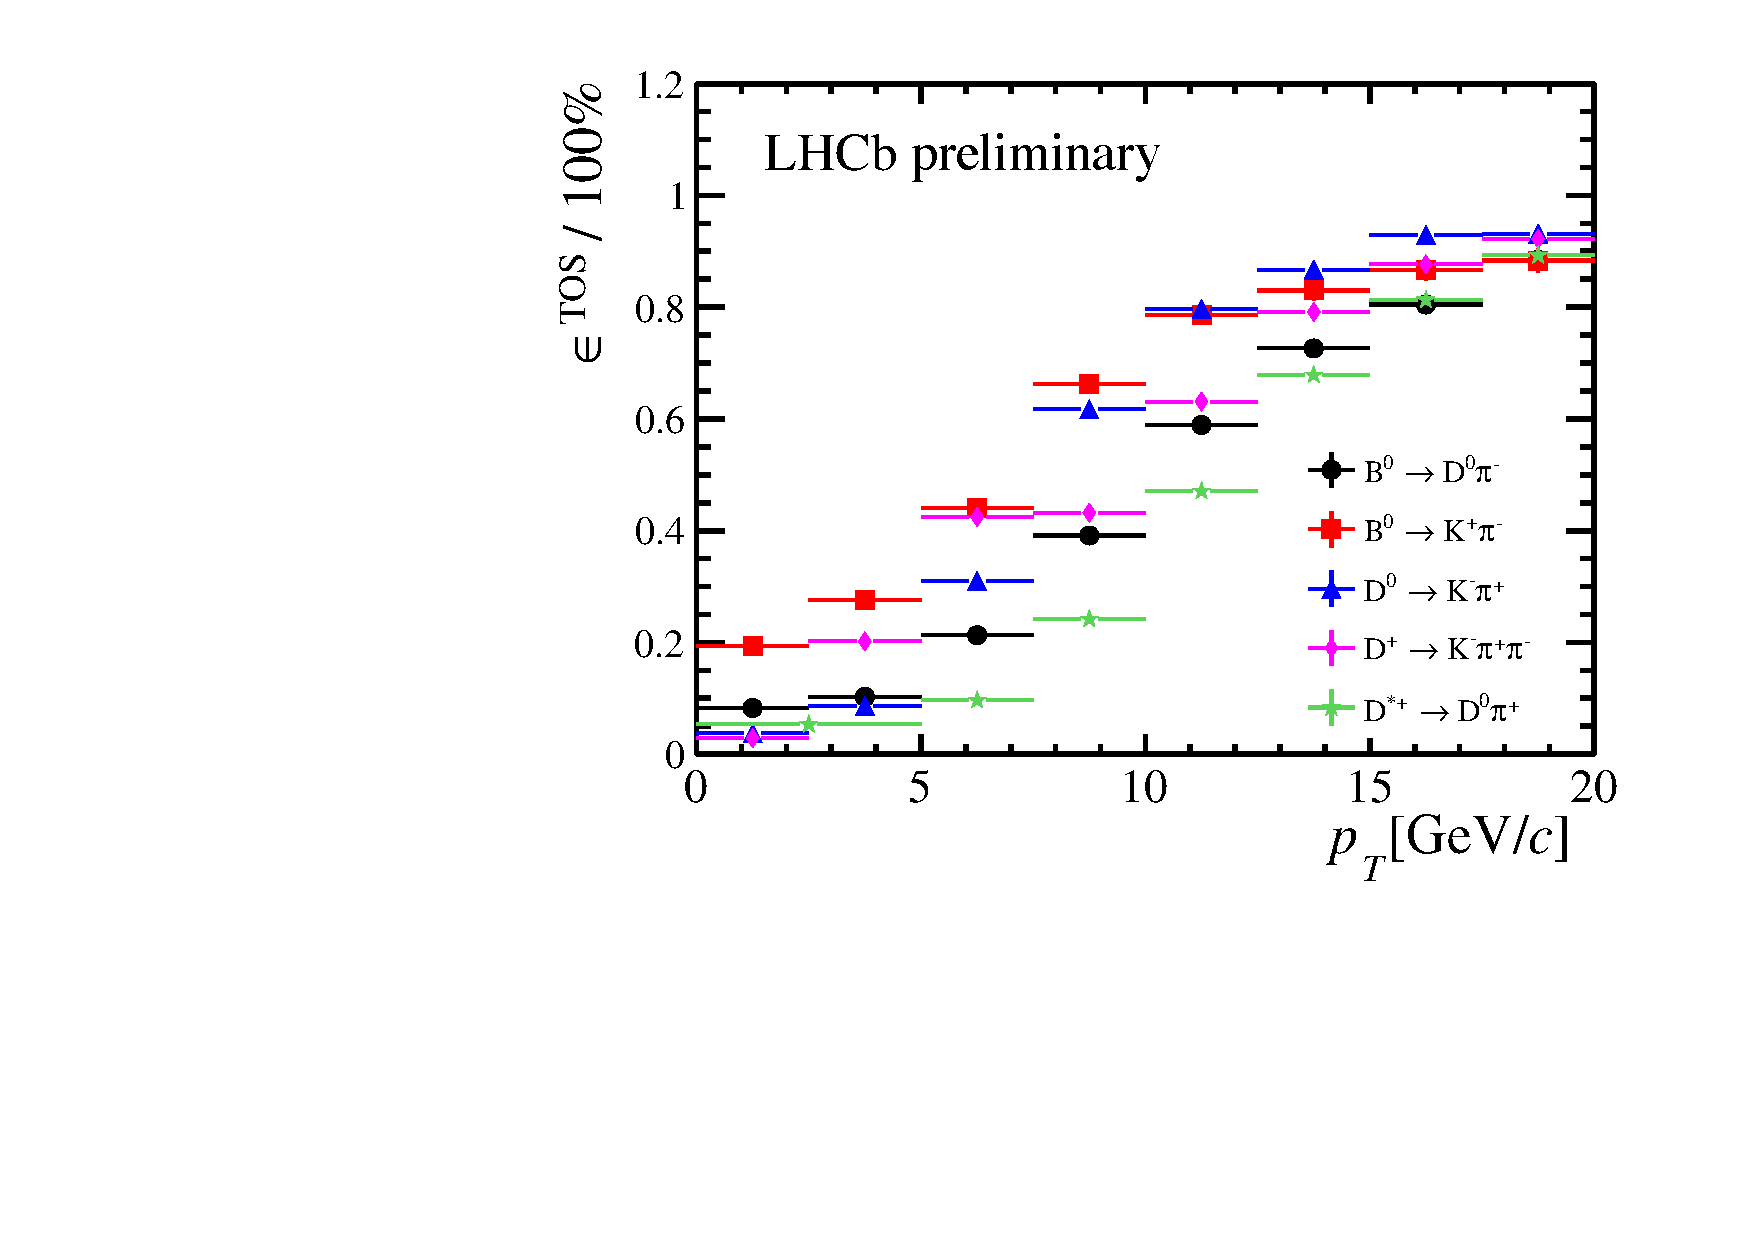
\includegraphics[width = 0.5\textwidth]{figs/detector/Fig21_L0Hadron_PT.pdf}\put(-50,90){(b)}%
	%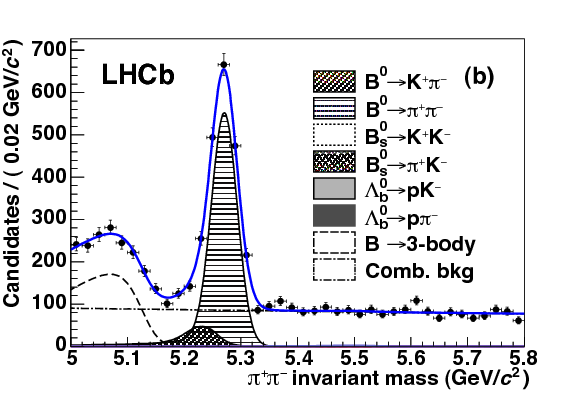
\includegraphics[width = 0.5\textwidth]{figs/detector/b2hhpid.png}%
	\caption{ (a) \Gls{TOS} efficiency as a function of $p_{T}$ for muon-based decisions. (b) \Gls{TOS} efficiency for different decays using L0 hadron trigger lines. Figures from \cite{Albrecht:2013fba}. }  
	\label{fig:L0Perf}
\end{figure}


 The software-based \Gls{HLT} then further reduces the rate from 1 \mhz down to $5$ \khz which can be recorded to long-term storage. The first stage of the \Gls{HLT}, (\Gls{HLT1}), performs limited track reconstruction and hence makes a decision based on the presence of charged particles in the event. \Gls{HLT1} uses \Gls{VELO} hits to reconstruct \Gls{PV}s and \Gls{VELO} tracks by using 3D pattern recognition. As \Gls{LHCb}'s primary mission is to study decays of hadrons containing $b$ and $c$ quark, \Gls{HLT1} will make decision based on the track being displaced (having high \Gls{IP}) with respect to the \Gls{PV}. For events selected by the \texttt{L0Muon}, an attempt is made to match the \Gls{VELO} tracks to hits observed in the vertical plane in the muon chambers, where the magnetic field of the dipole will not make them bend. By computing the track $\chi^2$, the potential muon track candidates are selected. Finally, the \Gls{VELO} tracks and muon tracks are extrapolated into the \Gls{OT} or \Gls{IT} trackers, allowing for so called \textit{forward tracking}, whereby $p$ and $p_{T}$ requirements are imposed to reduce processing time. Each track is then fitted with  a fast Kalman filter providing the $\chi^2$ of the fit. The corresponding performance of \Gls{HLT1} trigger lines are shown in~\autoref{fig:Hlt1Perf}(a)(b).


\begin{figure}[!h]
	\centering
	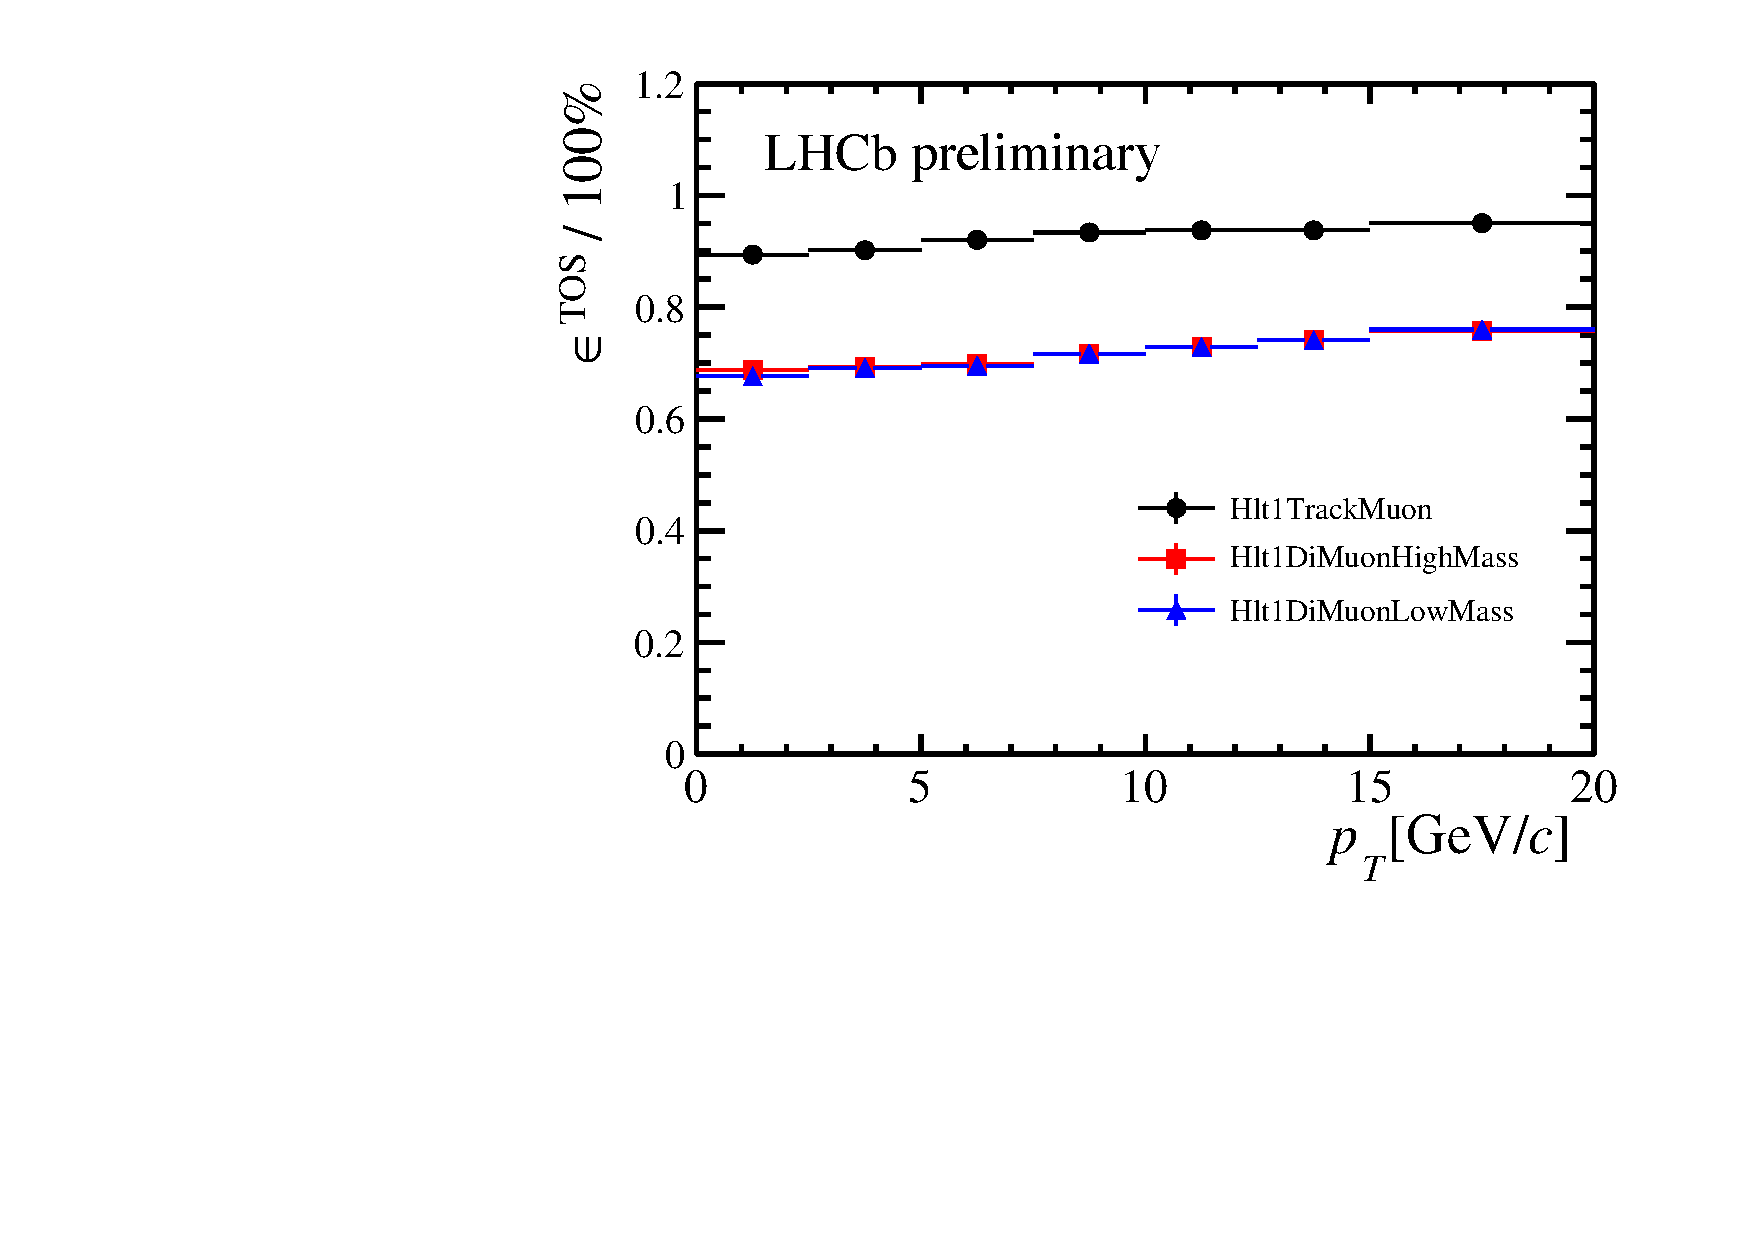
\includegraphics[width = 0.5\textwidth]{figs/detector/Fig3_Hlt1MuonEff_PT.pdf}\put(-50,140){(a)}%
	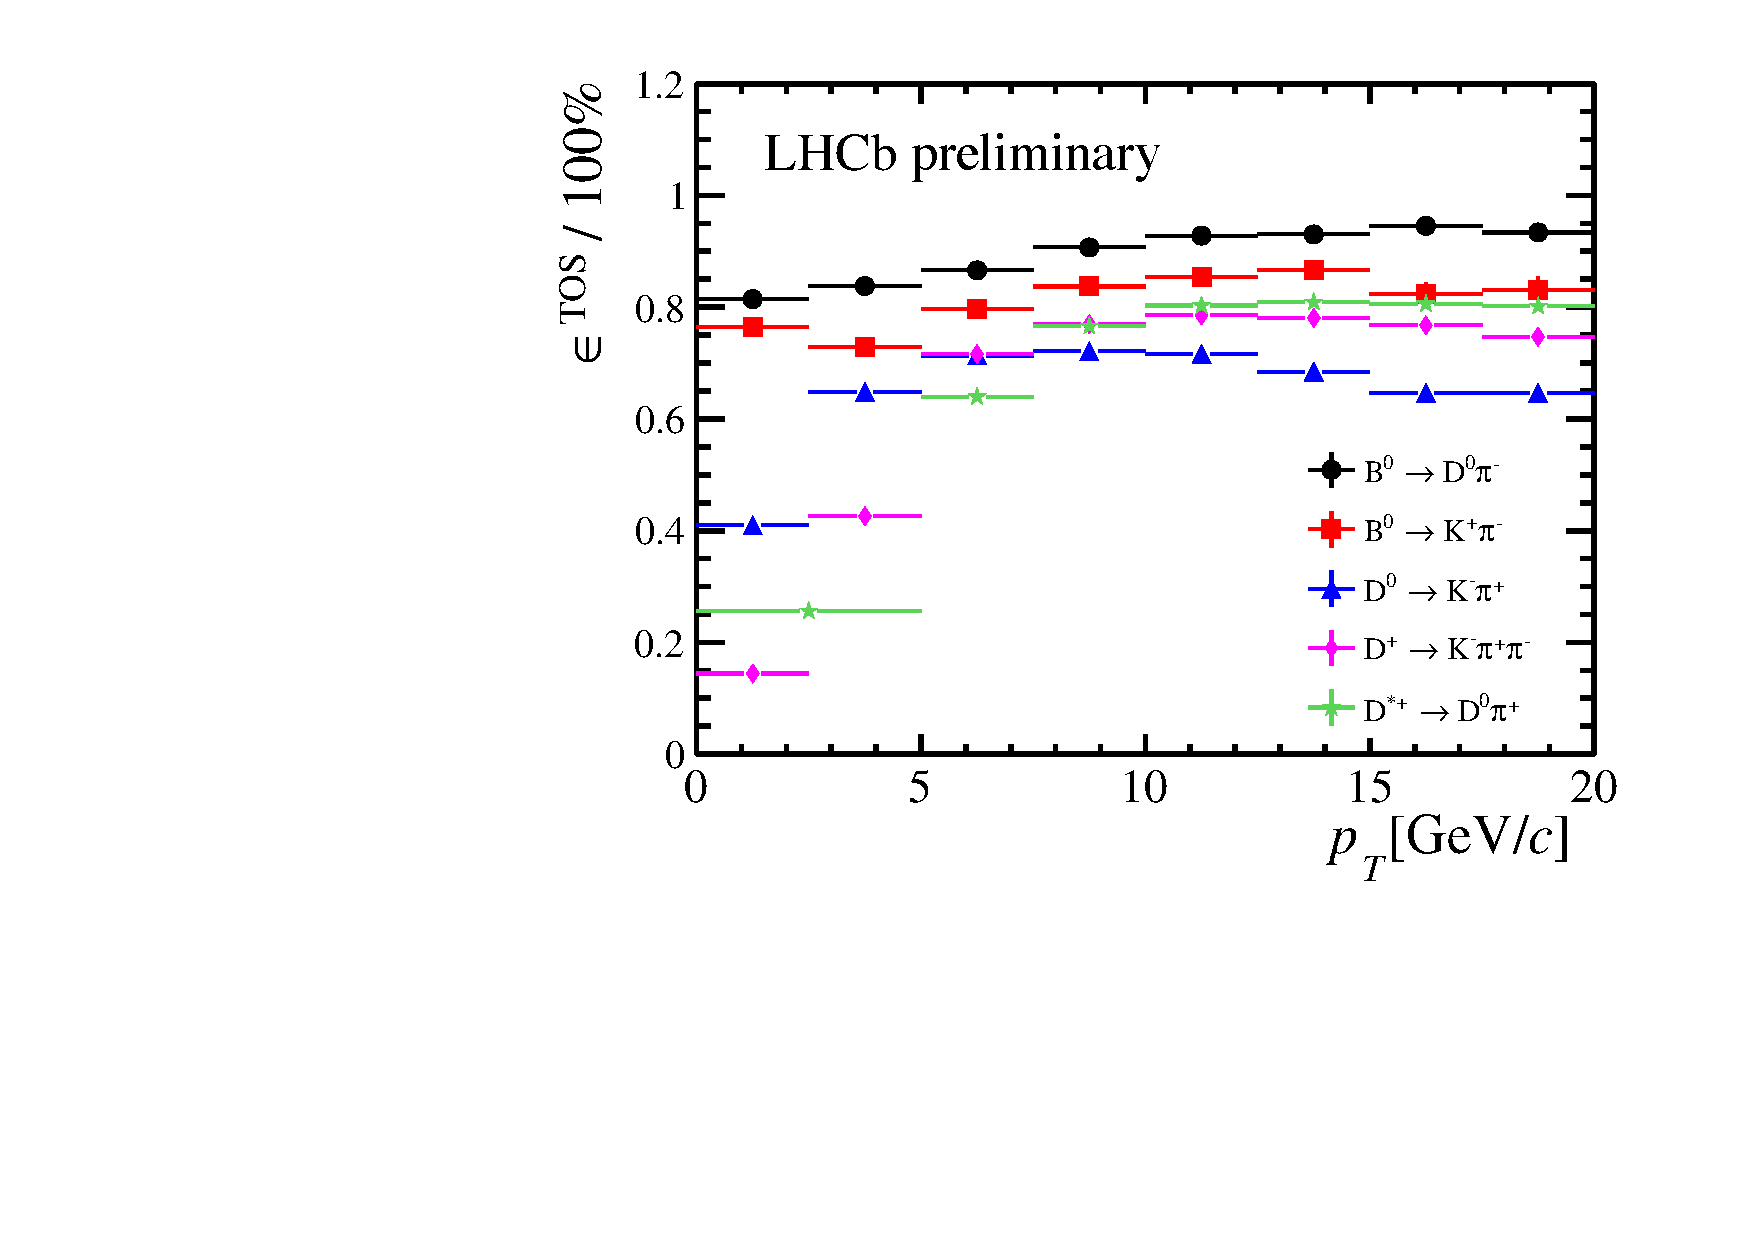
\includegraphics[width = 0.5\textwidth]{figs/detector/Fig5_Hlt1TrackAllL0_PT.pdf}\put(-50,140){(b)}%
	%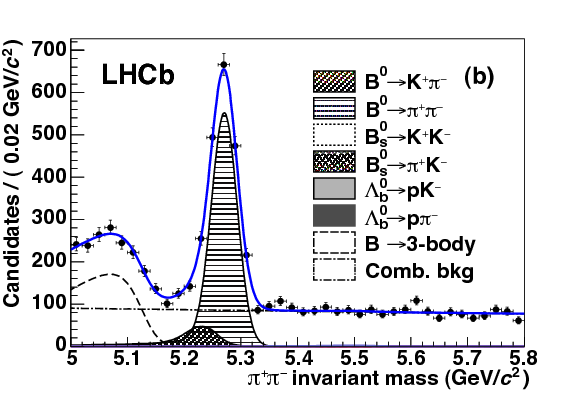
\includegraphics[width = 0.5\textwidth]{figs/detector/b2hhpid.png}%
	\caption{ \Gls{HLT1} efficiencies of the corresponding triggers using the same proxy as in~\autoref{fig:L0Perf}. Figures from \cite{Albrecht:2013fba}. }  
	\label{fig:Hlt1Perf}
\end{figure}

The second stage \Gls{HLT2} reduces the rate to 5 \khz that can be safely written to disk. \Gls{HLT2} consists of a series of decisions based on a full reconstruction of either groups of decays or specific decay modes. \textit{Topological triggers} exploit the vertex and track information (topology) of $b$-hadron decays. By employing multivariate techniques 2-,3- or 4-body decays that are well separated from the \Gls{PV} are reconstructed. To account for decays where a final state particle is not fully reconstructed, the corrected mass (will be defined in~\autoref{eq:corrm}) serves as an input variable in the the \Gls{BDT}. Dedicated lines are also written to reconstruct muon and dimuon channels allowing for both prompt $J/\psi$ and $B\rightarrow J/\psi X$ studies. Finally there are \textit{Exclusive triggers} concentrating on selecting events with $D$ mesons. They perform selection which is very similar to the offline selection but without \Gls{PID} cuts.% and with \textit{prescales} required, where only a certain fraction of events is allowed to pass through.



Between the Run \Rn{1} and Run \Rn{2} period there has been a change in how the software trigger operates, which can be seen in~\autoref{fig:TriggerChange}. As more computing resources were introduced for both \Gls{HLT1} and \Gls{HLT2}, \Gls{LHCb} took advantage in upgrading the trigger system by introducing an update of calibration and alignment constants of the relevant subdetectors before the data is sent to permanent disk. \textit{Online reconstruction}, defined as being produced at the trigger farm, became the same as the \textit{offline reconstruction}, defined as reconstruction made when data reached the permanent disk. Hence, there is enhancement of available information, such as the \Gls{PID} in the \Gls{HLT}, which can then be used at the trigger level. 


\begin{figure}[!h]
	\centering
	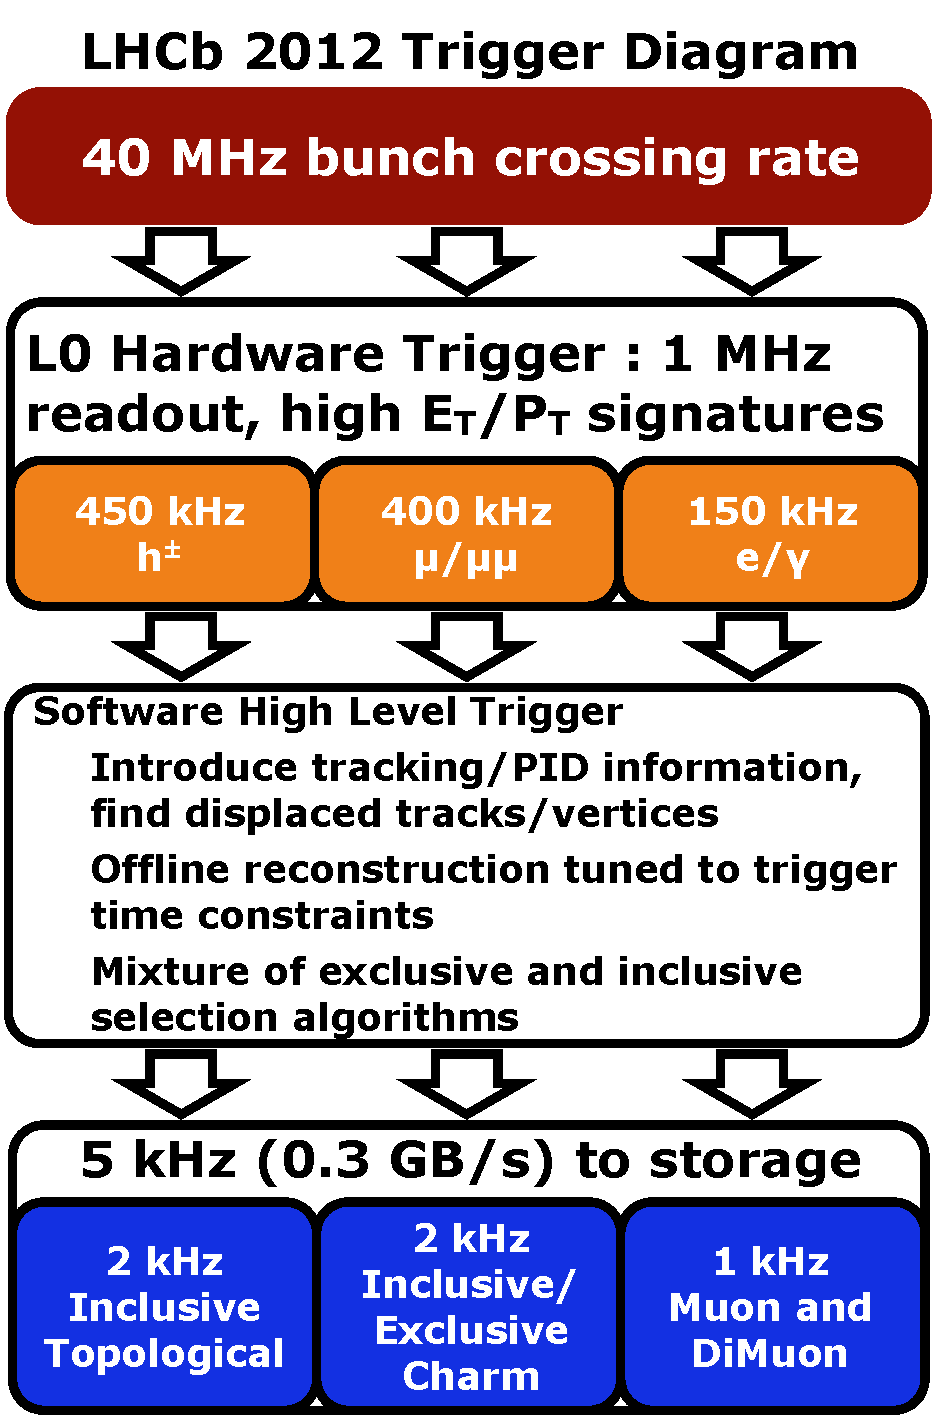
\includegraphics[width = 0.5\textwidth]{figs/detector/LHCb_Trigger_RunIAlg.pdf}%
	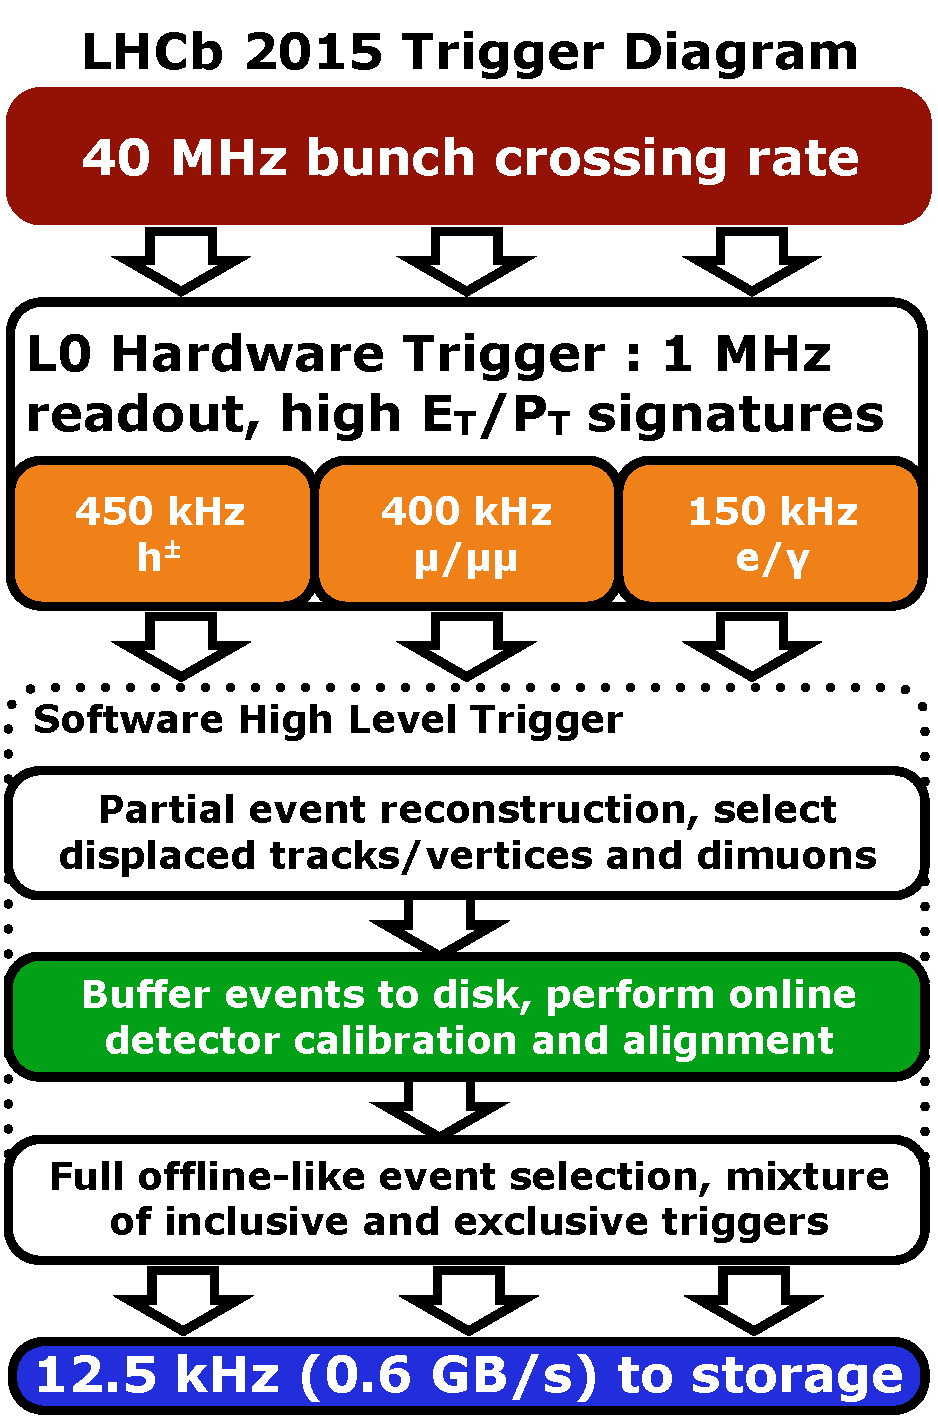
\includegraphics[width = 0.5\textwidth]{figs/detector/LHCb_Trigger_RunII.pdf}%
	%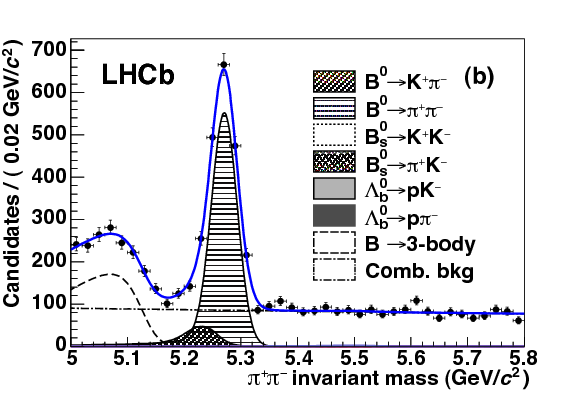
\includegraphics[width = 0.5\textwidth]{figs/detector/b2hhpid.png}%
	\caption{Trigger scheme differences between Run \Rn{1} and Run \Rn{2}. Figures from \cite{triggerscheme}.}  
	\label{fig:TriggerChange}
\end{figure}


\section{Simulation }
\label{simulationchap}
In order to optimise the event selections, determine efficiencies and model the backgrounds, a full Monte Carlo Simulation \Gls{MC} can be produced starting from simulation of the $pp$ collision to detector readout of the decay of interest produced. 
The $pp$ collisions within the \Gls{LHCb} configuration \cite{Belyaev:2011zza} are simulated with Pythia 6.4 \cite{pythia6} and Pythia 8.1 \cite{pythia8}. \Gls{LHCb} specific settings are mostly related to running conditions: luminosity, number of collisions per bunch crossing as well as contamination from other bunches, \textit{spill-over}. 

In the $pp$ collision, the $b$ and $c$ production mechanisms are simulated and then the following $b\bar{b}$ or $c\bar{c}$ pair is hadronized into hadrons of interest. In this thesis and the analysis presented, the \Bp meson is the hadron of interest. Hadrons are then further decayed using EVTGEN \cite{Lange:2001uf} into the chosen decay products. At this stage, different physics models or inputs from theory can be configured. % At the same time some initial CPU-friendly selection is established, usually requiring the hadrons to be contained within the forward detector's acceptance.
In order to account for the effects of \Gls{QED} radiative corrections, the PHOTOS \cite{photos} algorithm can be used. All of this combined establishes \textit{the generator-level simulation} of LHCb.


In the next phase, \textit{detector simulation}, the interactions of the all the particles with the detector, transport, as well as detector's response are simulated using the C++ GEANT4 toolkit \cite{Geant4},\cite{Agostinelli:2002hh}. \Gls{LHCb}'s interface to GEANT4 is detailed in Ref\cite{Clemencic:2011zza}. 

\subsection{Differences in Simulation and Data}
\label{detpid}
Despite the complexity and best intention of the \Gls{LHCb} simulation, there are several shortcomings that require corrections.
The most affected variables necessary for physics analyses that one needs to consider are \Gls{IP} resolution, track reconstruction efficiencies, \Gls{PID} variables and track occupancy.

The \Gls{IP} resolution shows a better trend in the simulation then in the data due to the mismodelling of the material description of the \Gls{VELO} simulation. As shown in~\autoref{fig:IPRES}(a)(b)  the \Gls{IP} resolution does greatly differ depending the variation of material density of \Gls{VELO}. Around $\phi=\pm\pi/2$, where the two \Gls{VELO} parts overlap, the material difference causes the discrepancy. It can be corrected either by reweighting to data or by smearing the resolution with a Gaussian distribution.

\begin{figure}[!h]
	\centering
	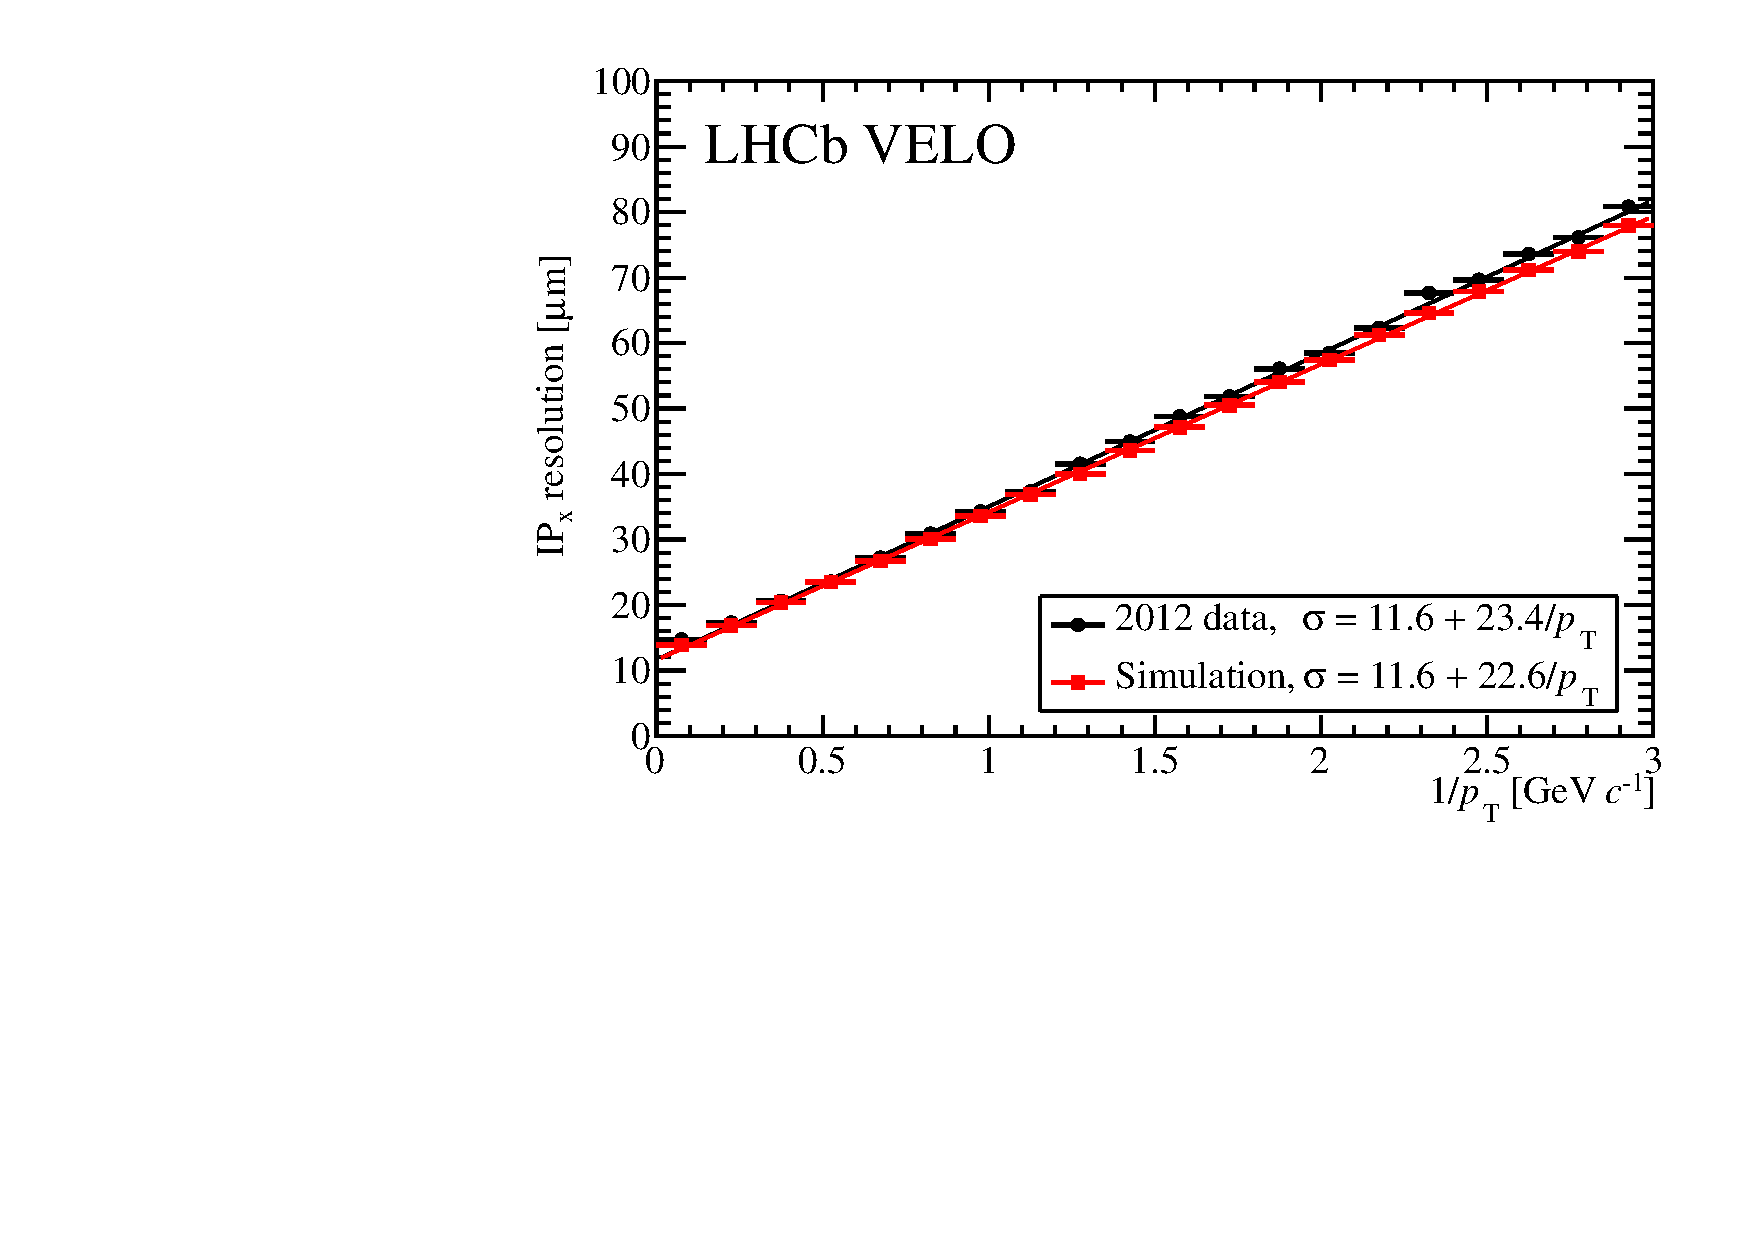
\includegraphics[width = 0.5\textwidth]{figs/detector/IPXRes-Vs-InversePT-Compare2012DataToMC.pdf}\put(-50,60){(a)}%
	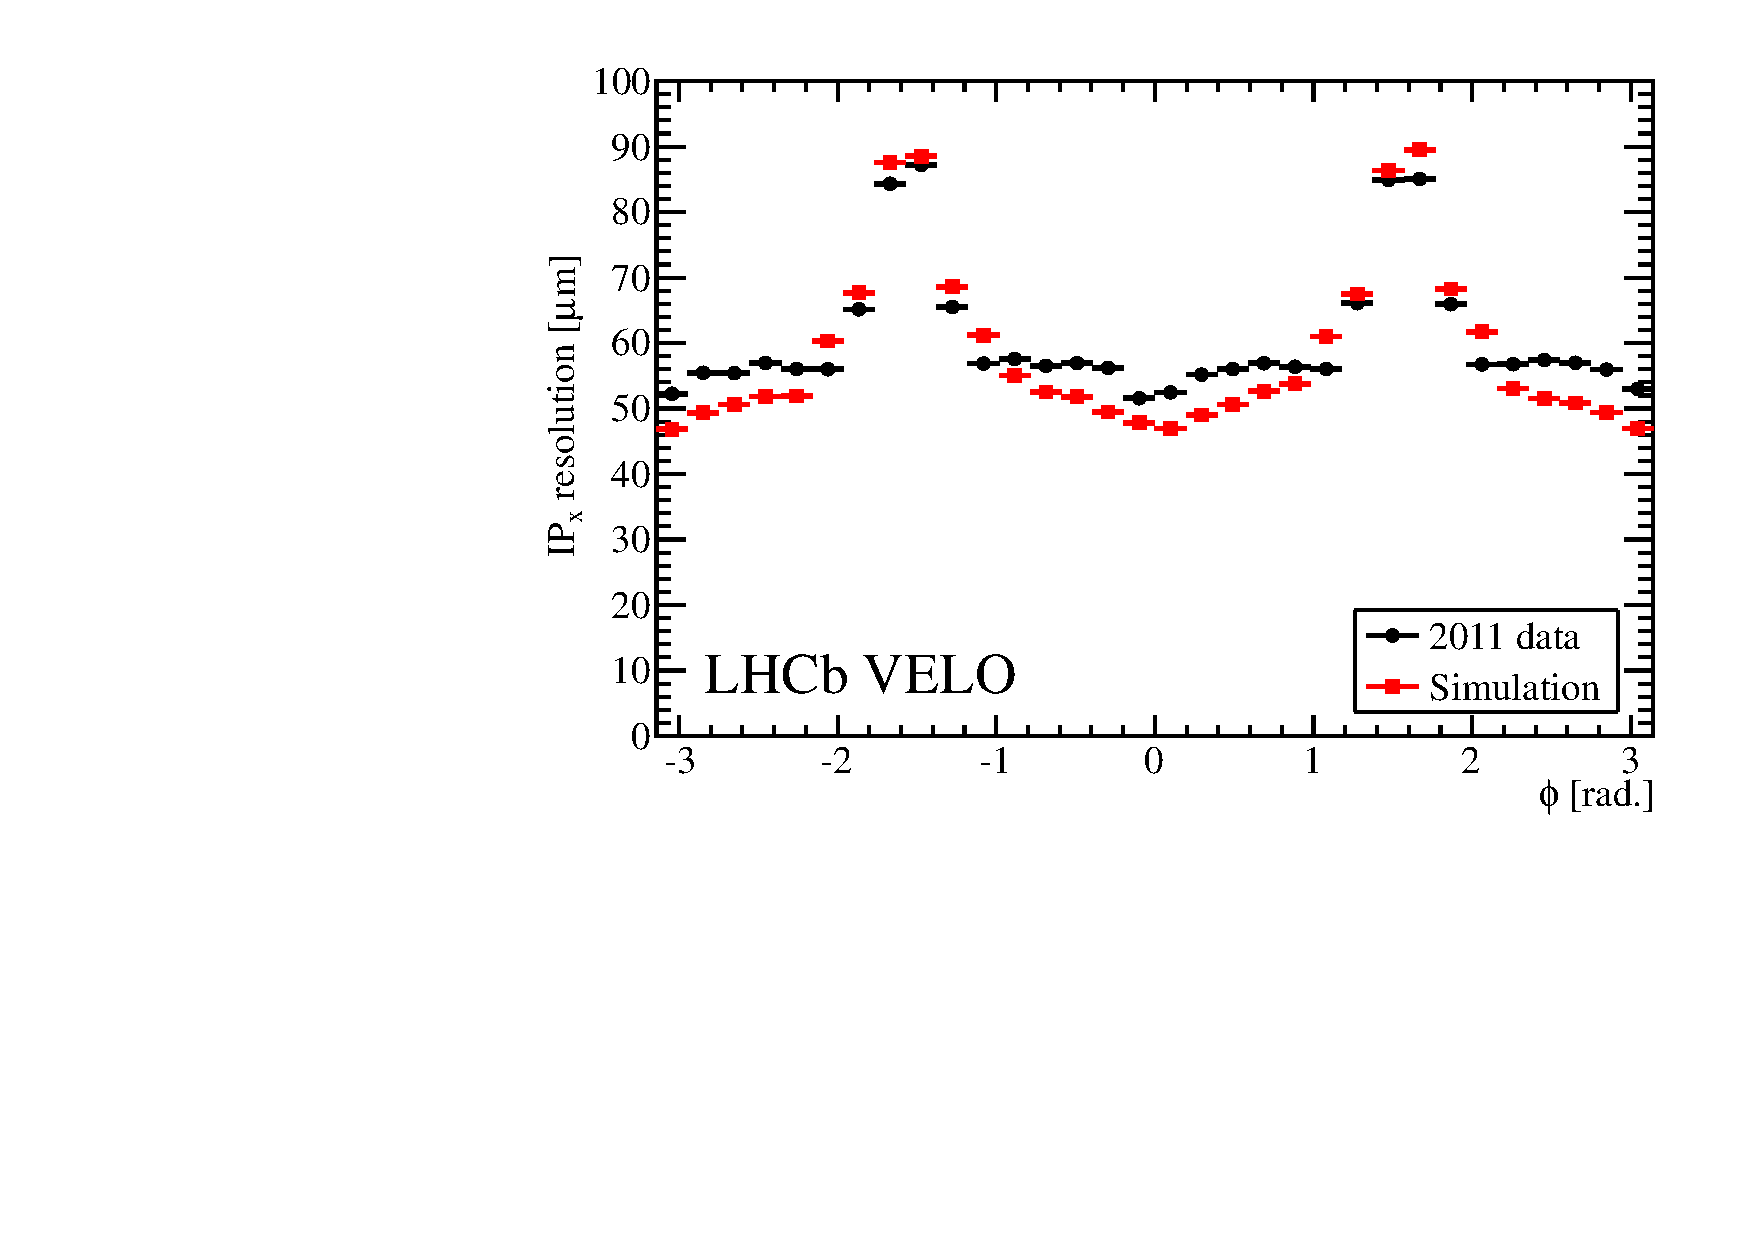
\includegraphics[width = 0.5\textwidth]{figs/detector/IPXRes-Vs-Phi-Compare2011DataToMC.pdf}\put(-50,60){(b)}%
	\caption{ (a) \Gls{IP} resolution in x-direction comparing the data and simulation output for 2012 data-taking period. (b) \Gls{IP} resolution in x-direction comparing the data and simulation output for 2011 data-taking period as a function of angle, $\phi$. Figures from \cite{LHCbVELOGroup:2014uea}. }  
	\label{fig:IPRES}
\end{figure}


Track reconstruction efficiency is also not reproduced very well in certain kinematical bins, again due to modelling of scattering interactions.

The most critical problem that needs to be addressed in the presented analysis are the inaccuracies of the \Gls{PID} variables, which are mismodelled in the simulation. The origin of this problem arises as a consequence of much lower estimate of low momentum tracks in the detector making the photoelectron background underestimated. This results in better performance of separation power in simulation and is corrected using data calibration. 

Therefore the \gls{PID} efficiency is usually obtained from data. More specifically, this is done by using high-yield and relatively background-free calibration channels, where the species of the particle can be deduced from kinematics of the decay. Standard set of these channels are "housed" in a \texttt{PIDCalib} package \cite{Anderlini:2202412}. In this package, \gls{PID} efficiency can be computed in a given kinematic region of interest. 


\chapter{Handling of Trimuon Correlations at LHCb}
\label{chap:trimuon}


\textit{This chapter discuss issues associated with three muons passing through the detector. Two collimated muons may traverse through the same parts of the detector if they have the same charge, causing problems in resolving their individual tracks. Therefore, ghosts and clones are much more likely to occur. In LHCb, a plethora of muon \Gls{PID} variables are used to suppress these types of spurious tracks. However, the usage of \gls{PID} variables in an analysis in \gls{LHCb} brings its own challenges. As the simulation is not able to estimate \gls{PID} efficiencies correctly, most of the \gls{PID} efficiencies are taken from control samples. New control samples for \Bmumumu are considered as the \Gls{PID} efficiencies depend strongly on the number of muons in the detector and in the standard misID control samples there is just a single muon in each event.}

\color{black}

\section{Muon PID Variables}
\label{otherpid}
In addition to the muon identification variables mentioned in~\autoref{muonID}, there is a further set of criteria for selecting muons. In this section a summary of the variables used in the analysis of the \Bmumumu is discussed.

\subsection{Binary Muon PID Variables }
Similar to \texttt{isMuon} shown in~\autoref{tab:ismuontab}, there are more binary variables, such as \texttt{isMuonTight}, that can help with classification of muons. As its name suggests, \texttt{isMuonTight} has stronger conditions to satisfy as compared to \texttt{isMuon}. 

In each muon station (\gls{muonstation}) a field of interest, \gls{FOI} is defined as %a function of momentum $p$ in a following way:
\begin{equation}
	FOI_{x,y}=\rho^{0}_{x,y}+\rho^{1}_{x,y}\cdot \exp \left(\frac{\rho^{2}_{x,y}\cdot p}{\gevc} \right),
\end{equation}
where $x,y$ are the dimensions perpendicular to the direction of the beam, $p$ is momentum of the muon, $\rho^{i}_{x,y}$ are three dimension-dependent parameters tuned to give the best performance, by maximizing efficiency to misID rate.

When a muon passes through the detector, it leaves hits ($h_{x,y}$ coordinate) in a pad with size $pad_{x,y}$ of each muon station. From the tracks formed in the tracking part of the detector, coordinates $E_{x,y}$ are obtained by extrapolating the tracks into the muon stations. The hits are considered to be within the \gls{FOI} if they satisfy the condition that $|| h_{d} - E_{d} || < FOI_{d} \cdot pad_{d}$ for both d={x,y}. 

\color{black}

The detector information is read out in the $x$ and $y$ direction separately. The pad slicing according to this read-out scheme is known as \textit{physical} slicing of pads. However, as seen in~\autoref{fig:pads}, the overlapping $x$ and $y$ \textit{physical} pads can be grouped into \textit{logical} pads, which give information about $x$ and $y$ simultaneously. This leads to two groups of hits according to pad type: uncrossed hits - registered within \textit{physical} pads only, and crossed hits - given by \textit{logical} pads. Whereas \texttt{isMuon} only requires positive decision from uncrossed hits, \texttt{isMuonTight} requires positive decision based on crossed hits. 


\begin{figure}[!h]
        \centering
        %
\includegraphics[width = 0.3\textwidth]{figs/trimuon/poze.jpg}
        \includegraphics[width = 1.0\textwidth]{figs/trimuon/fig2.pdf}
        \caption{Schematic view of the muon station slicing into x-y pads. This is the left quadrant of the M1 station, showing decreasing granularity of the muon stations away from the beam pipe. This figure has been taken from \cite{LHCb-DP-2012-002}. M1R1 is the innermost region and M1R4 is the outermost region of the M1 station. }
        \label{fig:pads}
\end{figure}

\subsection{Muon PID Variables Based on Sharing Hits }
\label{bugs}

Another way of identifying muon tracks is based on the variable, \texttt{nShared}, which identifies the number of tracks with shared hits in the muon stations. For each hit within the \gls{FOI} of an extrapolated track, the \texttt{nShared} algorithm will check whether any other track was built using the given hit. In this case, the \texttt{nShared} variable of the muon track which has the bigger distance between the extrapolation coordinates and the hit coordinates is increased by 1. Hence this integer \gls{PID} variable helps suppressing \textit{ghost} tracks and \textit{clones} if no tracks have hits in common with the owner of the track (\texttt{nShared=0}).

%\subsection{Different \texttt{nShared} definitions for Run \Rn{1} and Run \Rn{2}
%To make sure that muons for \Bmumumu are not coming from these spurious tracks,  \texttt{nShared==0} for all three muons is required. These three muon tracks will not to share hits in muon stations with any other downstream or long tracks. In analysing data, there were features in the Muon ID alghorithm, software that calculates most of muon \gls{PID} variables, which changed between Run \Rn{1} and Run \Rn{2} and will be discussed in greater detail, as it impacts the selection performed for \Bmumumu search.
The muon identification software algorithms evolved significantly between the processing of Run \Rn{1} and Run \Rn{2} data. This included bug fixes, improvements and the introduction of new bugs. In the \Bmumumu analysis, this has to be taken into account.


The first feature that is different between Run \Rn{1} and Run \Rn{2} arises from the calculation of the distance between the extrapolation and the hit in \texttt{nShared} algorithm.
In \textit{Stripping 21} (where \textit{stripping} is a preselection) used for 2012 and \textit{21r1} used for 2011 data, it was discovered that the distance between an extrapolated track and a hit was wrongly calculated. This mistake was corrected before \textit{Stripping 23}, used for analysing 2015 data. 

Secondly, information from the M1 station was used to calculate distances, even though M1 information is not usually used for the Muon ID algorithms.  For analysts, this feature was present across all reconstruction software, meaning that simulation and data is affected in the same way.

In \textit{Stripping 23}, the Muon ID algorithm was rewritten to adapt to the parallelisation that needs to be done in order to meet the criteria for the upgrade of \gls{LHCb}. There were two mistakes introduced prior to 2015 data taking.
Firstly, an array was defined with 4-elements $[0,3]$ to store information about $x$ and $y$ coordinates of the hits. However, an iteration occurred by filling elements 1 to 4 of the array (M2-M5 station) resulting in a 5-element array where the 0-th element was not filled. Despite this, it turns out to be well-behaved and has no impact on physics.

Further in the process, however, this information is used to calculate the sum and average of distances per station between the hits and extrapolations. This algorithm again iterates over $[0,3]$ arrays, meaning that no information is used from the M5 muon station. This obviously has an effect, but again it is consistent across the versions of the reconstruction software used for the processing of Run \Rn{2} data.

%\newline Summary of these features can be found in \href{https://indico.cern.ch/event/612764/contributions/2567244/attachments/1449649/2234804/20170426\_nShared.pdf}{\color{blue} in this presentation} 
The interplay between all these features for \bjpsimumuk decays, can be seen in~\autoref{fig:nSharedvar}, which sees a shift in distribution of \texttt{nShared} for 2016 data taking, making the muons less isolated.

\begin{figure}[h!]
\centering
\includegraphics[width=0.5\linewidth]{trimuon/plotvariablewantlogtruemu1_nSharedJPSIKMC.pdf}\put(-40,133){(a)}
\includegraphics[width=0.5\linewidth]{trimuon/plotvariablewantlogtruemu1_nSharedJPSIKDATA.pdf}\put(-40,133){(b)}
	\caption{(a) \texttt{nShared} variable distribution for the positive muon in \bjpsimumuk decays in (a) simulation and (b) data. Different stripping versions corresponding to 2012 (\textit{Stripping 21}), 2011 (\textit{Stripping 21r1}), 2016 (\textit{Stripping 26}) data-taking are shown. The distributions are normalised to have the same area. There is shift of distribution in \textit{Stripping 26} towards less isolated tracks. The proportion of muon tracks that share no other hits with other tracks is smaller, whereas the proportion of the tracks sharing hits with other muon track is increasing.}
\label{fig:nSharedvar}
%\vspace*{-1.0cm}
\end{figure}

Using the same calibration channels as in~\autoref{muonperf}, misID and ID rates can be seen in~\autoref{fig:nSharedRun1andRun2}. As the tracks tend to be less isolated in \textit{Stripping 26} used for 2016 data, typical of non-signal like events, the misID rate is expected to be higher for the same working point (ID efficiency). While the issues highlighted here can be fixed with a reprocessing of the data, this is not expected to happen before 2019 or 2020.

\begin{figure}[h!]
\centering
%\includegraphics[width=0.52\linewidth]{compareRun1and2016selection/final_comparedirectly2012vs2015_nolog.pdf}%
\includegraphics[width=0.7\linewidth]{trimuon/final_pretty_2016_pion.pdf}
	\caption{ID and misID probabilities from standard calibration datasets from 2012 (\textit{Stripping 21}) and 2016 (\textit{Stripping 26}), binned using the default 2-dimensional binning scheme in momentum $p$ and pseudorapidity $\eta$. In this plot, ID and misID rates in the central bin of $\eta$, 2.375<$\eta$<3.25, and the first and second bin in $p$ are compared. This demonstrates that for the same pion ID efficiency, the misID rate is significantly higher in 2016 data.}
\label{fig:nSharedRun1andRun2}
%\vspace*{-1.0cm}
\end{figure}

\subsection{Muon PID Variables Based on Regression Techniques }
\label{muonPIDprobnn}
Similar to the DLLmu variable in~\autoref{muonID}, which combines all the information from the detector into a global likelihood, it is possible to feed all the different variables to a neural network, which can then produce an output corresponding to the probability of a particle to be of a certain species. \texttt{Probnn${x}$}, where $x$ is the species of interest, is calculated and can be used also for muon identification. Compared to $\rm{DLLx}$ variables, \texttt{Probnn${x}$} variables tend to have smaller correlation with the kinematics of the particle, and hence are more useful with decays where particles are soft, such as \Bmumumu. As with any machine learning algorithm, the selection of both the training sample and the input variables are important. In Run \Rn{1}, there were two tunings (trainings) introduced \texttt{V2} and \texttt{V3}, with more input variables in \texttt{V2}. Depending on the species of particles, \texttt{V2} or \texttt{V3} performed better. In the analysis of \Bmumumu, \texttt{Probnn${x}\_$V2} is used.


\section{Clones}
\label{cloniatkos}
When analysing decays with two muons of opposite charge, the \gls{LHCb} magnet bends these two muons in two opposite directions. With two muons of the same sign, the muons will instead bend in the same direction and can stay close together in both the tracking system and the muon detectors. This causes trouble for the tracking algorithm as it distinguishes these two tracks less well. It is even possible that these two same sign muon tracks are not genuine tracks, but rather subtracks or a copy of another track, \textit{clone tracks}. Two tracks are clones if they share at least 70\% of the hits in the \gls{VELO} and at least 70\% of the hits in the other T-stations. Of course, once it is established that two tracks share this percentage of hits, it has to be established which track is the clone track. This decision is based on the total number of hits and the track $\chi^{2}$ per number of degrees of freedom of the fit (\texttt{ndof}) (\gls{trackchi2ndof}) comparison of the two tracks.   


\begin{figure}[h!]
\centering
\includegraphics[width=0.5\linewidth]{trimuon/compnice_even_nicer_ONLY_STACKED_HIST_VisibleCorrM.pdf}\put(-50,133){(a)}
\includegraphics[width=0.5\linewidth]{trimuon/compnice_even_nicer_ONLY_STACKED_HIST_CorrM.pdf}\put(-50,133){(b)}
	\caption{(a) Visible and (b) corrected mass of \Bmumumu candidates in 2012 data where all the muons have the same charge. Clear fake peaks, arising from the correlation of several effects in the detector can be seen. }
\label{fig:Clones}
%\vspace*{-1.0cm}
\end{figure}


In search for \Bmumumu, two muons have the same charge, and hence are affected by the \textit{clones}, which needs to be understood. In a control sample from data corresponding to 2012 data-taking period, which have three muon candidates of the same charge, the effect is even more prominent and can create potentially \textit{fake peaks} in visible mass spectrum. \textit{Clones} peak at well defined visible mass 
\begin{equation}
	M_{B}=\sqrt{(3 \times M_{\mu})^{2}}\approx 318 \mevcc
	\label{eq:invmass}
\end{equation}

Once translated into corrected mass (will be defined in~\autoref{eq:corrm}), these \textit{fake peaks} are smeared and look like genuine resonances with resolution as seen in~\autoref{fig:Clones}.  


The shape emulating a genuine resonance arises as a collective effect from vertexing, tracking and trigger selection. As there are three parallel tracks, the vertex of the system is not well defined. However, the vertex fitting of the \gls{PV} and secondary (decay) vertex (\gls{SV}) is functional and \gls{vertexchi2ndof} (the $\chi^{2}$ of the vertex per degree of freedom in a vertex fit) is good as these tracks are subtracks of each other. The distance between \gls{PV} and \gls{SV} is defined as flight distance (\gls{FD}). However, \textit{clones} can be differentiated by the position of the decay vertex of $B$,~\autoref{fig:ClonesFD} as well as the transverse position of the track in the tracking, \gls{OT} as seen in~\autoref{fig:ClonesOT}.

\begin{figure}[h!]
\centering
\includegraphics[width=0.5\linewidth]{trimuon/VertexInfoClone.pdf}\put(-50,133){(a)}
\includegraphics[width=0.5\linewidth]{trimuon/VertexInfoNoClone.pdf}\put(-50,133){(b)}
	\caption{(a) Clone and (b) no clones flight distance properties. It can be seen that \textit{clone} tracks have their decay vertex placed at the end of the detector, whereas regular good tracks will decay within the \gls{VELO}.}
\label{fig:ClonesFD}
%\vspace*{-1.0cm}
\end{figure}


\begin{figure}[h!]
\centering
\includegraphics[width=0.5\linewidth]{trimuon/OTxandyClone.pdf}\put(-50,133){(a)}
\includegraphics[width=0.5\linewidth]{trimuon/OTxandyNoClone.pdf}\put(-50,133){(b)}
	\caption{The difference in the \gls{OT} detector between (a) clones and (b) real tracks in the \Gls{OT} at the distance 9450 \mm along the \gls{LHCb}. \textit{Clones} are concentrated along the inner edge of the \gls{OT}. Good muon tracks will cover most of \gls{OT} evenly.}
\label{fig:ClonesOT}
%\vspace*{-1.0cm}
\end{figure}


With this typical path for the clones there is a fixed angle of the clones through the detector (the angle between the muon momentum and the z-axis), which is calculated using information from \gls{OT} as

\begin{equation}
        \arctan(\theta)=\arctan\Big(\frac{\gls{FD}\ radius}{\gls{FD}\ distance\ along\ z}\Big)=\arctan\Big(\frac{200\ \mm\ (\autoref{fig:ClonesOT})}{8500\ \mm}\Big) = 0.023 \rm{rad}. 
\end{equation}


With the \texttt{L0Muon} $p_{T}$ threshold of 1.76 \gevc for 2012 \cite{Albrecht:2013fba}, the typical momentum from about 75  to 120 \gevc is yielded because

\begin{equation}
        p=1.76\gevc/\sin\bigg(\arctan\Big(\frac{200\ \mm}{8500\ \mm}\Big)\bigg).
\end{equation}

The angle between $B$ flight and trimuon momentum vector, \gls{DIRA}, will also be fixed and have typical value of 0.7 \mrad as seen in~\autoref{fig:ClonesDIRA}.

\begin{figure}[h!]
\centering
\includegraphics[width=0.5\linewidth]{trimuon/compnice_even_nicer_ONLY_STACKED_HIST_oneFILE_BplusDiraclone.pdf}\put(-50,133){(a)}
\includegraphics[width=0.5\linewidth]{trimuon/compnice_even_nicer_ONLY_STACKED_HIST_oneFILE_BplusDiranoclone.pdf}\put(-50,133){(b)}
        \caption{(a) Peaking clone distribution is visible as all of \textit{clone} tracks are collinear compared to (b) smooth no clone distribution for \gls{DIRA}.}
\label{fig:ClonesDIRA}
%\vspace*{-1.0cm}
\end{figure}


Hence, missing $p_{T}$ in the direction of the flight can be calculated using \gls{DIRA} and typical $p$,

\begin{equation}
	p_{T}=100\gevc \times \sin(0.0007)=0.7\gevc,
	\label{eq:mispt}
\end{equation}
corrected mass $M_{\rm{corr}} = \sqrt{{M}^{2} + |p^{2}_{T}|} + |p_{T}| = 4.2 \gevcc$, using missing $p_{T}$ from~\autoref{eq:mispt} and visible mass of \textit{clones} from~\autoref{eq:invmass}.


In order to suppress these tracks in analysing \Bmumumu, where two muons have the same sign, any distinguishing features mentioned could be used. But the most powerful \gls{PID}-wise is requiring \texttt{nShared=0} in Run \Rn{1}, as this requirement removes all of the clones, as seen in~\autoref{fig:ClonesnShared}. 
For Run \Rn{2}, due to the introduced bugs, such strong requirement would harm signal efficiency too much so combination of \texttt{nShared<2} and \texttt{isMuonTight=1} is applied instead.
%\textit{this should remove them as well as nShared is increased for the non-owner track only- i assume that owner track will be that of nshared=0. I.e below nShared==3 for the clones, so for two muons nShared==2 so if there are two tracks, is ok}
\color{black}
%\newline In order to keep the signal efficiency high in 2016 data, as shown in Table ~\ref{tab:Reason}, softer condition ,$\texttt{nShared}<2$, is applied.

\begin{figure}[h!]
\centering
\includegraphics[width=0.5\linewidth]{trimuon/compnice_even_nicer_ONLY_STACKED_HIST_oneFILE_sumnSharedclone.pdf}\put(-50,133){(a)}
\includegraphics[width=0.5\linewidth]{trimuon/compnice_even_nicer_ONLY_STACKED_HIST_oneFILE_sumnSharednoclone.pdf}\put(-50,133){(b)}
	\caption{(a) Clone and (b) no clone distribution for sum of all muon \texttt{nShared}. Since in this case the clones are of each other, for the clones there is clear peak at three. }
\label{fig:ClonesnShared}
%\vspace*{-1.0cm}
\end{figure}

\section{Probability of \mb{K/\pi \rightarrow \mu} Misidentification at LHCb }

Usually, in order to estimate background coming from misidentification of particles as muons in the detector, data samples with particles of known (non-muon) type are identified from the kinematics of the decay chains. From these samples, probabilities of mis-identification are derived as discussed in~\autoref{RICHperf}. However, the three muon signature will induce problems for \gls{PID} variables that are correlated with the number of muons in the detector and specific data samples that incorporates this correlation have to be used for measuring the mis-identification probability.

\subsection{Specific Control Sample for \mb{K/\pi \rightarrow \mu} MisID Rates }
\label{extraction}
A platform that \gls{LHCb} analysts usually use to obtain the misID and ID efficiencies, as described in~\autoref{RICHperf}, is known as the \texttt{PIDCalib} package \cite{Anderlini:2202412}. It contains samples where the identity of the particle is know purely from kinematics.  In this \texttt{PIDCalib} package, such a control same for $K/\pi$ is obtained from $D^{*+}(\rightarrow D^{0}(\rightarrow \underline{K^{+} \pi^{-}}) \pi^{+})$ decays. These statistically populated background-free \textit{sWeighted} samples\cite{sPlot}, for which it is possible to extract misID and ID rates as a function of kinematics given certain \gls{PID} criteria, do not have other muons in the final state. 

More specifically, the topology of the misID background component, which is two real muon tracks with an additional \textit{fake} muon track is very different to the \texttt{PIDCalib} sample $D^{*+}(\rightarrow D^{0}(\rightarrow \underline{K^{+} \pi^{-}}) \pi^{+})$, where there are no muons in the final state.

%This influences the rest of the misID rates as some of the \gls{PID} variables are strongly correlated with number of muons in the decay, due to the fact that the mis-identified particle can share hits with other muons in the rest of the decay. This should be reflected mostly in high momenta region, where the three particles tend to be collimated and share hits most often.

For this reason, $B^{0} \rightarrow J/\psi(\rightarrow \mu^{+} \mu^{-}) K^{*}(\rightarrow \underline{K^{+} \pi^{-}})$ is used instead. While not as common as $D^{*+}(\rightarrow D^{0}(\rightarrow \underline{K^{+} \pi^{-}}) \pi^{+})$ decay, it still has high statistics and can be isolated with little background. It mimics the two real muon plus fake muon correctly and will be used to obtain pion and kaon misID probabilities.
% This is a clean decay that can be fit to obtain \textit{sWeights} to measure PID efficiencies. Moreover, its the signal topology and kinematics are much closer to the actual mis-ID backgroundcomponent than
% that of the PIDCalib control samples.

\subsection{Selection for \mb{B^{0} \rightarrow J/\psi(\rightarrow \mu^{+} \mu^{-}) K^{*}}  }
Data samples for each year of data taking were obtained from the \textit{stripping line} (set of preselection cuts) dedicated to look for this type of decay. The sample can be used for misID studies of the hadrons as no particle identification is applied on them. Some initial selection was applied together with the more stringent \Bmumumu selection.  The trigger criteria were applied on the $J/\psi$ candidate rather than on the $B$ candidate. The full additional selection is summarized in~\autoref{tab:cleanjpsikst} is used.


\begin{table}[h!]
\begin{center}
\begin{tabular}{ l  l }
\toprule
Idea  & Cut  \\ \hline
ID $K^{*}$ & $|$ M(K$\pi$) - M$_{PDG}(K^{∗}_{0})$ $|$ $ <100$ \mevcc \\
%Compatible with \texttt{PIDCalib} & \color{black} &  for K,$\pi$ , p$_{T} > 250$ \mevc\\
%Compatible with \texttt{PIDCalib} &  for $\mu$ , p$_{T} > 800$ \mevc \\
Muon swap veto & $|$ M((h $\rightarrow \mu$ )$\mu$) - M$_{PDG}$(J/$\psi$)$|$ $> 60$ \mevcc \\
	Veto $B^{+}\rightarrow K^{+}\mu^{+}\mu^{-}$ & max(M($K^{+}\mu^{+}\mu^{-}$)), M($(\pi^{+} \rightarrow K^{+})\mu^{+}\mu^{-})$) $< 5100$ \mevcc\\
Veto $B^{0}_{s}\rightarrow \phi \mu^{+} \mu^{-} $ & M(K($\pi\rightarrow$ K)) $>1040$ \mevcc \\
	ID muons & \texttt{Probnnmu}$>$0.5 \\
\hline
For kaon misID rates: & \\
ID pion & DLLK $<$ 0 DLLp $<$ 0 and \texttt{IsMuon==0}\\
\hline
For pion misID rates: & \\
ID kaon & DLLK $>$ 0 and DLLK-DLLp $>$ 0 and \texttt{IsMuon==0} \\
\bottomrule
\end{tabular}
\end{center}
\caption{Offline selection for $B^{0} \rightarrow J/\psi(\rightarrow \mu^{+} \mu^{-}) K^{*}$ decay.}
\label{tab:cleanjpsikst}
\end{table}


\subsection{Fitting Strategy for \mb{B^{0} \rightarrow J/\psi(\rightarrow \mu^{+} \mu^{-}) K^{*}}}
After the selection, the residual background needs to be modelled. The signal component, $B^{0} \rightarrow J/\psi K^{*}$, is obtained by fixing the shape from simulation apart from the mean $\mu$ and the width $\sigma$. It is fitted with a double-sided Ipatia function \cite{Santos:2013gra} (more in~\autoref{IP}).

Background that peaks in the upper mass sideband, coming from heavier $B^{0}_{s}$, $\bar{B}^{0}_{s} \rightarrow J/\psi (\rightarrow \mu^{+} \mu^{-}) K^*(\rightarrow \underline{K^{+} \pi^{-}})$ is also modelled using simulation, using the same function as signal but with $\mu$ offset by the difference between the known $B^{0}_{s}$ and $B^{0}$.

It is also possible that kaons and pions are swapped between themselves. Background coming from $K \leftrightarrow \pi$ swaps is modelled from simulation where the mass hypotheses were swapped. Its distribution is fitted with a double sided Crystal Ball function \cite{Skwarnicki:1986xj} (more in~\autoref{CB}).

Possibility of misidentified background comes from decay of $\Lambda_{b} \rightarrow K^{-} p \mu^{+} \mu^{-}$ where the proton is misidentified as a pion. This background is modelled from simulation and fitted with a \texttt{RooKeys} probability density function (PDF) (more in~\autoref{RK}).

Finally a combinatorial component is modelled by the exponential function.


The mass of the $J/\psi$ was \textit{constrained} to its nominal mass, a procedure also known as a \textit{mass constraint}. It yields new estimates for track parameters of the final state particles, from which a new kinematic refit is done.

In order to obtain $K/\pi$ misID probabilities an unbinned maximum likelihood fit to the $\mu^{+} \mu^{-} \pi^{+} K^{-}$ mass between 5150 - 5450 \mevcc was performed. This fit with parameters listed in~\autoref{tab:floatingparsummarylol} give the yield of all the components. 

\begin{table}[H]
\centering
\begin{tabular}{ l  l }\toprule
Fit Parameter & Status  \\ \hline
	\multicolumn{2}{c}{Yields} \\ \hline
$N_{B^{0} \rightarrow J/\psi K^{*}}$ (Signal)  &  Free \\
$N_{K \pi swaps}$ & Free\\
$N_{\Lambda_{b} \rightarrow J/\psi K^{-} p}$ & Free\\
$N_{B_{s} \rightarrow J/\psi K^{*}}$ & Free \\
$N_{Combinatorial}$ & Free\\
\hline
	\multicolumn{2}{c}{Signal Shape Parameters} \\
\hline
$\mu_{B^{0} \rightarrow J/\psi K^{*}}$ & Constrained from signal MC\\
$\sigma_{B^{0} \rightarrow J/\psi K^{*}}$ & Constrained from signal MC\\
Others & Fixed from MC\\
\hline
$K\ \pi\ swaps$ Shape Parameters & Fixed from MC \\
\hline
$\Lambda_{b} \rightarrow J/\psi K^{-} p$ Shape Parameters & Fixed from MC \\
\hline
	\multicolumn{2}{c}{${B_{s} \rightarrow J/\psi K^{*}}$ Shape Parameters} \\\hline
$\mu_{B_{s} \rightarrow J/\psi K^{*}}$ & Offset by $\mu_{B^{0} \rightarrow J/\psi K^{*}}$ \\
Others & Fixed from signal MC \\
\hline
	\multicolumn{2}{c}{Combinatorial Shape Parameters}  \\
\hline
exponential par.  & Free\\
\bottomrule
\end{tabular}
\caption{Summary of the fit parameters and individual component constraints for $B^{0} \rightarrow J/\psi K^{*}$ fit.}
\label{tab:floatingparsummarylol}
\end{table}






The actual determination of the misID rate was obtained using a statistical method of background subtraction, known as the \textit{sPlot} technique \cite{sPlot}, as the samples are not fully background-free. The same method is also used in the \texttt{PIDCalib} package. In the \textit{sPlot} method, the invariant mass distribution is fitted with no \gls{PID} applied and each event is assigned \textit{sWeights}, probabilities that a given event is a signal-like or a background-like. Then, through the \textit{sPlot} technique, background is subtracted. Signal component can then be calculated by summing all the \textit{sWeights} for all the candidates. The misID probabilities are finally obtained by dividing this signal component sum of \textit{sWeights} with \gls{PID} applied and with no \gls{PID} applied. This misID probabilities are then considered within some kinematic partitioning, bins of $p,\eta$. 

\color{black}

The misID rate was also cross-checked with another method, the \textit{fit twice method}. This is because the \textit{sPlot} technique relies on the fact that there is no correlation between the control variables ($p$, $\eta$) and the discriminating variable (invariant mass) for both signal and background. This assumption may not be true, especially for background, and it can introduce biases.

The \textit{fit twice method} consists of fitting $B^{0} \rightarrow J/\psi(\rightarrow \mu^{+} \mu^{-}) K^{*}$ before and after the \gls{PID} requirement in a given kinematic ($p$, $\eta$) bin separately. MisID probabilities are then obtained as the ratio of signal yields arising from these two fits.


It was shown that these two methods yields very similar results, hence,
for purposes of the \Bmumumu analysis the \textit{sWeight} values will be used. Fits to Run \Rn{1} and 2016 data for both kaon and pion misID studies can be seen in ~\autoref{fig:JpsiKst}.
%IF YOU WANT TO CHANGE THE PLOTS HAVE A LOOKHERE /vols/lhcb/ss4314/fitjpsikst/fitjpsikst_idKAON_includeswaps_automatize_master_sweight_cinMuonAc_NOghostprob_mydefbin_onnlyONEbinINeta_2016_newPIDopt/NOFCME/ there is mainPLOTonly function
\begin{figure}[H] 

\center
\includegraphics[width = 0.5\textwidth]{figs/trimuon/jpsikst/2011/plotJpsiKstFitLogyPretty_nicecolor_2011_KAONMISID.pdf}\put(-150,100){(a) 49K events }%
\includegraphics[width = 0.5\textwidth]{figs/trimuon/jpsikst/2011/plotJpsiKstFitLogyPretty_nicecolor_2011_PIONMISID.pdf}\put(-150,100){(b) 46K events}
\newline
\includegraphics[width = 0.5\textwidth]{figs/trimuon/jpsikst/2012/plotJpsiKstFitLogyPretty_nicecolor_2012_KAONMISID.pdf}\put(-150,100){(c) 112K events }%
\includegraphics[width = 0.5\textwidth]{figs/trimuon/jpsikst/2012/plotJpsiKstFitLogyPretty_nicecolor_2012_PIONMISID.pdf}\put(-150,100){(d) 107K events}
\newline
\includegraphics[width = 0.5\textwidth]{figs/trimuon/jpsikst/2016/plotJpsiKstFitLogyPretty_nicecolor_2016_KAONMISID.pdf}\put(-150,100){(e) 205K events}%
\includegraphics[width = 0.5\textwidth]{figs/trimuon/jpsikst/2016/plotJpsiKstFitLogyPretty_nicecolor_2016_PIONMISID.pdf}\put(-150,100){(f) 161K events}
	\caption{Fit to constrained $J/\psi(\rightarrow \mu^{+} \mu^{-}) K^{*}(\rightarrow \pi^{+} K^{-})$ mass with all the components for (a)(b) 2011, (c)(d) 2012, (e)(f) 2016. On the left, fit to data with pion ID (giving kaon misID probabilities), on right data with kaon ID (pion misID rates).}
\label{fig:JpsiKst}
\end{figure}

\subsection{Results of \mb{B^{0} \rightarrow J/\psi(\rightarrow \mu^{+} \mu^{-}) K^{*}} Control Sample for \mb{K/\pi \rightarrow \mu} MisID Rates }
\label{ratiatkos}
%\color{red} Using the \textit{sWeight} method, misID rates for kaons and pions can be obtained. In order to rule out that any disagreement of \gls{PID} performance is caused by the fraction of the real kaon and pions tracks within the muon fiducial area, following check is performed. For both control samples, kaon sample from the $D^{*+}(\rightarrow D^{0}(\rightarrow \underline{K^{+} \pi^{-}}) \pi^{+})$ events and the kaon sample from the $B^{0} \rightarrow J/\psi(\rightarrow \mu^{+} \mu^{-}) K^{*}$ events, the probability of correctly identifying kaon is computed, given that only extrapolated tracks that fall within muon acceptance are considered. This is achieved by requiring that given kaon track has \texttt{InMuonAcceptance==1.0}. It can be seen in ~\autoref{tab:ROE} that the ID performance is the same across nearly all of the momentum range for kaons, showing that the fraction of the kaons tracks within muon acceptance is very similar. The same check was performed for pions tracks as well. 

%\color{black}
%
%\begin{table}[h!]
%%\small
%\begin{center}
%\begin{tabular}{ l  H  H  c   }\toprule
%	$p$ range [\mevc] & $D^{*+}(\rightarrow D^{0}(\rightarrow \underline{K^{+} \pi^{-}}) \pi^{+})$  & $B^{0} \rightarrow J/\psi(\rightarrow \mu^{+} \mu^{-}) K^{*}(\rightarrow \underline{K^{+} \pi^{-}})$  & $B^{0} \rightarrow J/\psi(\rightarrow \mu^{+} \mu^{-}) K^{*}(\rightarrow \underline{K^{+} \pi^{-}})/D^{*+}(\rightarrow D^{0}(\rightarrow \underline{K^{+} \pi^{-}}) \pi^{+})$  \\	
%\hline
%3000 - 6000 &   0.77$\pm$0.0016 & 0.83$\pm$0.0047 & 1.1$\pm$0.0065 \\
%6000 - 9300 &   0.93$\pm$0.00030 & 0.95$\pm$0.0019 & 1.0$\pm$0.0020 \\
%9300 - 10000 &  0.96$\pm$0.00037 & 0.97$\pm$0.0031 & 1.0$\pm$0.0033 \\
%10000 - 12600 &  0.97$\pm$0.00014 & 0.97$\pm$0.0017 & 1.0$\pm$0.0017 \\
%12600 - 15600 &   0.98$\pm$0.00011 & 0.97$\pm$0.0017 & 0.99$\pm$0.0018 \\
%15600 - 17500 &   0.98$\pm$0.00013 & 0.96$\pm$0.0024 & 0.98$\pm$0.0025 \\
%17500 - 21500 &   0.98$\pm$8.9e-05 & 0.96$\pm$0.0018 & 0.98$\pm$0.0018 \\
%21500 - 27000 &   0.98$\pm$7.8e-05 & 0.96$\pm$0.0018 & 0.98$\pm$0.0019 \\
%27000 - 32000 &   0.98$\pm$8.8e-05 & 0.96$\pm$0.0024 & 0.98$\pm$0.0025 \\
%32000 - 40000 &  0.98$\pm$8.0e-05 & 0.96$\pm$0.0022 & 0.98$\pm$0.0022 \\
%40000 - 60000 &  0.97$\pm$7.5e-05 & 0.95$\pm$0.0021 & 1.0$\pm$0.0022 \\
%60000 - 70000 &  0.96$\pm$0.00016 & 0.96$\pm$0.0043 & 1.0$\pm$0.0046 \\
%70000 - 100000 &  0.95$\pm$0.00013 & 0.94$\pm$0.0044 & 0.99$\pm$0.0046 \\
%\bottomrule
%\end{tabular}
%\end{center}
%	\caption{\color{red} It is necesarry as this is unrelated to following figures  \color{black}\texttt{K$\_$InMuonAcc==1.0} shows the interpolation of $K$ tracks into muon chambers. It can be seen that both samples agree with each other very well, meaning that measured misID rate is done for the same fraction of considered tracks. This measurement is done in a pseudorapidity region $1.5<\eta<5.0$.}
%\label{tab:ROE}
%\end{table}

Using the \textit{sWeight} method, misID rates for kaons and pions can be obtained. Two control samples that are analysed and compared are $D^{*+}(\rightarrow D^{0}(\rightarrow \underline{K^{+} \pi^{-}}) \pi^{+})$ events (standard \texttt{PIDCalib} sample), where there are no other muons in the decay, and $B^{0} \rightarrow J/\psi(\rightarrow \mu^{+} \mu^{-}) K^{*}(\rightarrow \underline{K^{+}\pi^{-}})$ events, where there are two real muons along with kaons or pions. Selecting only tracks that are within the muon fiducial region for both pion and kaon allows to perform study of the misID probabilities within the two calibration samples. In ~\autoref{fig:JpsiKnew}(a), the $\pi \rightarrow \mu$ misID probability for different \gls{PID} hypotheses from $B^{0} \rightarrow J/\psi(\rightarrow \mu^{+} \mu^{-}) K^{*}(\rightarrow K^{+}\pi^{-})$ sample is studied. As it can be noticed, the more stringent the muon selection on the pion track, the lower the probability of misidentification.

In general the agreement between the two samples is good in the low momentum regions as shown in ~\autoref{fig:JpsiKnew}(b). These pions are softer and hence they will spread out more in the magnetic field, causing less interference with two other real muons in decay. However, in the high momentum region, the pion will follow a path through the muon system that is more similar to the path of the muon of the same charge in the $B^{0} \rightarrow J/\psi(\rightarrow \mu^{+} \mu^{-}) K^{*}$ decay. The influence of the two other real muons in a high momenta the region will lead to bigger disagreement as these two real muons leave hits in the muon chambers close to the collimated pion track, making the rate of \texttt{IsMuon==1.0} (pink) higher. 


%By selection tracks within the muon fiducial region for both pion and kaon allows to perform study of the misID probabilities with the two calibration samples.
%In ~\autoref{fig:JpsiKnew}, the $\pi \rightarrow \mu$ misID probability for different \gls{PID} hypotheses are studied. As it can be noticed, the more stringent the muon selection on the pion track, the lower the probability of misidentification. 

%On the right, the ratio of the misID probabilities between two samples show particular trend. 


\begin{figure}[h!]
\center
%\includegraphics[width = 0.55\textwidth]{figs/trimuon/jpsikst/2012/Visualize_Weights_KaonMisid_2011_small.pdf}\put(-50,133){(a)}%
		\includegraphics[width = 0.5\textwidth]{figs/trimuon/jpsikst/2012/Visualize_Weights_PionMisid_2012_small_thesis.pdf}\put(-50,133){(a)}
%		\newline
%		\includegraphics[width = 0.55\textwidth]{figs/trimuon/jpsikst/2012/Visualize_Weights_KaonMisid_small.pdf}\put(-50,133){(c)}%
		\includegraphics[width = 0.5\textwidth]{figs/trimuon/jpsikst/2012/Visualize_Ratios_PionMisid_small_thesis.pdf}\put(-50,133){(b)}
		\newline
%		\includegraphics[width = 0.55\textwidth]{figs/trimuon/jpsikst/2012/Visualize_Weights_KaonMisid_2016_small.pdf}\put(-50,133){(e)}%
		\includegraphics[width = 1.0\textwidth]{figs/trimuon/jpsikst/2012/Visualize_Weights_PionMisid_2012_small_thesis_legend.pdf}
		\caption{(a) $\pi \rightarrow \mu$ misID probabibility for different PID requirements obtained using $B^{0} \rightarrow J/\psi(\rightarrow \mu^{+} \mu^{-}) K^{*} (\rightarrow {K^{+} \pi^{-}} )$ for 2012 data. (b) This is compared to the standard \texttt{PIDCalib} $D^{*+}(\rightarrow D^{0}(\rightarrow K^{+} \pi^{-}) \pi^{+})$ sample. }
		\label{fig:JpsiKnew}
\end{figure}

%Using the \textit{sWeight} method, misID rates for kaons and pions can be obtained. Two control samples that are analysed are $D^{*+}(\rightarrow D^{0}(\rightarrow \underline{K^{+} \pi^{-}}) \pi^{+})$ events and $B^{0} \rightarrow J/\psi(\rightarrow \mu^{+} \mu^{-}) K^{*}$ events.
%In general the agreement is good in the low momentum regions between the two samples as shown in ~\autoref{fig:JpsiKnew}. These pions are softer and hence they will spread out more in the magnetic field, causing less interference with other two real muons in decay. However, in high momentum region, the pion will follow a path through the muon system that is more similar to the path of the muon of the same charge in the $B^{0} \rightarrow J/\psi(\rightarrow \mu^{+} \mu^{-}) K^{*}$ decay. The influence of other two real muons in high momenta region will lead to bigger disagreement as these two real muons leave hits in the muon chambers close to the collimated pion track, making the rate of \texttt{IsMuon==1.0} (pink) is higher. 

This disagreement is decreased by requiring \texttt{nShared==0.0} (blue), as having two other collimated muons to share hits will be more likely. The effect of other \gls{PID} variables can also be seen, but it is harder to interpret as these depend on several variables.

Even though this disagreement is decreased, for the high momenta region $\pi \rightarrow \mu$ (~\autoref{fig:JpsiKnew}) and $K \rightarrow \mu$ (~\autoref{fig:JpsiKaonnew}) rate is 2 to 3 times higher with additional two real muon tracks. Such disagreement is significant and if the misID rates from the standard control samples were to be used to be parametrically applied on samples to estimate the misID background, there would be an underestimate the misID component by the same factor.

In conclusion, it was shown that the standard misID samples are not good proxies for estimating the misID probabilities as there is interference from two other muons in the event. Instead, the misID probabilities that are used in calculations for the misID background for \Bmumumu are obtained from \textit{Sweighted} $B^{0} \rightarrow J/\psi(\rightarrow \mu^{+} \mu^{-}) K^{*}$. Remaining effects of taking this sample for calibration are considered as a systematic uncertainty, with more details in~\autoref{misidfitstrat}.



\begin{figure}[h!]
\center
%\includegraphics[width = 0.55\textwidth]{figs/trimuon/jpsikst/2012/Visualize_Weights_KaonMisid_2011_small.pdf}\put(-50,133){(a)}%
		\includegraphics[width = 0.5\textwidth]{figs/trimuon/jpsikst/2012/Visualize_Weights_KaonMisid_2012_small_thesis.pdf}\put(-50,133){(a)}
%		\newline
%		\includegraphics[width = 0.55\textwidth]{figs/trimuon/jpsikst/2012/Visualize_Weights_KaonMisid_small.pdf}\put(-50,133){(c)}%
		\includegraphics[width = 0.5\textwidth]{figs/trimuon/jpsikst/2012/Visualize_Ratios_KaonMisid_small_thesis.pdf}\put(-50,133){(b)}
		\newline
%		\includegraphics[width = 0.55\textwidth]{figs/trimuon/jpsikst/2012/Visualize_Weights_KaonMisid_2016_small.pdf}\put(-50,133){(e)}%
		\includegraphics[width = 1.0\textwidth]{figs/trimuon/jpsikst/2012/Visualize_Weights_KaonMisid_2012_small_thesis_legend.pdf}
		\caption{(a) $K \rightarrow \mu$ misID probabibility for different PID requirements obtained using $B^{0} \rightarrow J/\psi(\rightarrow \mu^{+} \mu^{-}) K^{*} (\rightarrow {K^{+} \pi^{-}} )$ for 2012 data. (b) This is compared to the standard \texttt{PIDCalib} $D^{*+}(\rightarrow D^{0}(\rightarrow K^{+} \pi^{-}) \pi^{+})$ sample. }
		\label{fig:JpsiKaonnew}
\end{figure}

Due to the different \gls{PID} definitions of \texttt{nShared} between Run \Rn{1} and 2016, different \gls{PID} requirement are tested.  Results for $\pi \rightarrow \mu$ and $K \rightarrow \mu$ are summarized in~\autoref{fig:JpsiPionnew2016} and
~\autoref{fig:JpsiKaonnew2016}. The misID probabilities in 2016 for also show the same momentum dependent trend as in 2012. 



\begin{figure}[h!]
\center
%\includegraphics[width = 0.55\textwidth]{figs/trimuon/jpsikst/2012/Visualize_Weights_KaonMisid_2011_small.pdf}\put(-50,133){(a)}%
		\includegraphics[width = 0.5\textwidth]{figs/trimuon/jpsikst/2016/Visualize_Weights_PionMisid_2016_small_thesis.pdf}\put(-50,133){(a)}
%		\newline
%		\includegraphics[width = 0.55\textwidth]{figs/trimuon/jpsikst/2012/Visualize_Weights_KaonMisid_small.pdf}\put(-50,133){(c)}%
		\includegraphics[width = 0.5\textwidth]{figs/trimuon/jpsikst/2016/Visualize_Ratios_PionMisid_2016_small_thesis.pdf}\put(-50,133){(b)}
		\newline
%		\includegraphics[width = 0.55\textwidth]{figs/trimuon/jpsikst/2012/Visualize_Weights_KaonMisid_2016_small.pdf}\put(-50,133){(e)}%
		\includegraphics[width = 1.0\textwidth]{figs/trimuon/jpsikst/2016/Visualize_Weights_PionMisid_2016_small_thesis_legend.pdf}
		\caption{(a) $\pi \rightarrow \mu$ misID probabibility for different PID requirements obtained using $B^{0} \rightarrow J/\psi(\rightarrow \mu^{+} \mu^{-}) K^{*} (\rightarrow {K^{+} \pi^{-}} )$ for 2016 data. (b) This is compared to the standard \texttt{PIDCalib} $D^{*+}(\rightarrow D^{0}(\rightarrow K^{+} \pi^{-}) \pi^{+})$ sample. }
		\label{fig:JpsiPionnew2016}
\end{figure}


\begin{figure}[h!]
\center
%\includegraphics[width = 0.55\textwidth]{figs/trimuon/jpsikst/2012/Visualize_Weights_KaonMisid_2011_small.pdf}\put(-50,133){(a)}%
		\includegraphics[width = 0.5\textwidth]{figs/trimuon/jpsikst/2016/Visualize_Weights_KaonMisid_2016_small_thesis.pdf}\put(-50,133){(a)}
%		\newline
%		\includegraphics[width = 0.55\textwidth]{figs/trimuon/jpsikst/2012/Visualize_Weights_KaonMisid_small.pdf}\put(-50,133){(c)}%
		\includegraphics[width = 0.5\textwidth]{figs/trimuon/jpsikst/2016/Visualize_Ratios_2016_KaonMisid_small_thesis.pdf}\put(-50,133){(b)}
		\newline
%		\includegraphics[width = 0.55\textwidth]{figs/trimuon/jpsikst/2012/Visualize_Weights_KaonMisid_2016_small.pdf}\put(-50,133){(e)}%
		\includegraphics[width = 1.0\textwidth]{figs/trimuon/jpsikst/2016/Visualize_Weights_KaonMisid_2016_small_thesis_legend.pdf}
		\caption{(a) $K \rightarrow \mu$ misID probability for different PID requirements obtained using $B^{0} \rightarrow J/\psi(\rightarrow \mu^{+} \mu^{-}) K^{*} (\rightarrow {K^{+} \pi^{-}} )$ for 2016 data. (b) This is compared to the standard \texttt{PIDCalib} $D^{*+}(\rightarrow D^{0}(\rightarrow K^{+} \pi^{-}) \pi^{+})$ sample. }
		\label{fig:JpsiKaonnew2016}
\end{figure}


\chapter{Looking for \mb{\Bmumumu} Decays at LHCb}
\label{chap:sel}

\textit{In this chapter, the selection for the search of \Bmumumu decays at LHCb is presented. This search is challenging because of the rareness of its occurrence as well as the different backgrounds that can mimic its signature in the detector. Moreover, presence of of the invisible neutrino in the decay induces uncertainties into the reconstruction. This chapter concentrates on data selection which reduces background contamination. Normalisation channel along with its selection is also discussed. In the end, a method to improve sensitivity is introduced.}



\section{Topology of the \mb{\Bmumumu} Decay at LHCb}

Upon hadronisation from a $b\bar{b}$ pair, a \Bpm particle will travel around a centimetre in the laboratory frame of reference before it decays. This allows reconstruction of a primary vertex \gls{PV} and its decay vertex \gls{SV}. By joining these vertices, the direction as well as flight distance \gls{FD}, can be established. In order to infer information about the kinematic properties of the \Bpm meson, the decay products are studied. All three muons are used to reconstruct the visible four-momentum. By conservation of momentum, %with respects to the direction of the flight of \Bpm,
the neutrino is assigned all missing momentum transverse to the direction of the flight of the \Bpm meson. A schematic diagram of the decay topology can be seen in~\autoref{fig:sigtopolog}.

\begin{figure}[!h]
	\centering
	\includegraphics[width = 0.8\textwidth]{figs/sel/DecReco_fin.eps}
	\caption{Schematic view of the \Bmumumu decay. All charged particle tracks (in solid-blue) are combined into a four-vector representing the visible part of the decay (dashed-blue). Information about the invisible neutrino (dashed-red) is deduced from the conservation of momentum with respect to the direction of the flight of the \Bpm meson.}% Neglecting momentum component parallel to the direction of flight for neutrino, transverse component of momentum is given.}
	\label{fig:sigtopolog}
\end{figure}

Combining all information allows for reconstruction of the corrected mass that plays a similar role to invariant mass in fully reconstructed decays. It is defined as
%Invariant mass is usually used in \gls{LHCb} as the distribution from which the yield of a signal decay is determined through a fit. This particular quantity is used as it distinguishes well signal and background shapes with minimal modelling assumptions.
% defined as

\begin{equation}
	M_{\mathrm{corr}} = \sqrt{{M}^{2} + |p^{2}_{T}|} + |p_{T}|,
\label{eq:corrm}        
\end{equation}	
where the $M^{2}$ is the invariant visible mass squared and $p^{2}_{T}$ is the missing momentum squared transverse to the direction of the $B^{+}$ meson flight. The corrected mass of the \Bpm meson will be denoted as $M_{\mathrm{B_{corr}}}$. The $M_{\mathrm{corr}}$ is equal to the true mass if the missing part of the decay has zero mass and has no momentum along the $\Bpm$ flight direction. Otherwise, $M_{\mathrm{corr}}$ is below the $\Bpm$ mass.
%\begin{equation}
%M_rm{{B_{corr}}} = \sqrt{M_{\mu^{+} \mu^{-} \mu^{+}}^{2} + |p_{T}|} + |p_{T}|,
%\end{equation}	

$M_{\mathrm{corr}}$ can be thought of as the minimal correction to the visible mass to account for the missing neutrino information. The resolution on the corrected mass (the uncertainty of this quantity) hence becomes a critical quantity that needs to be understood. As the method of reconstruction of corrected mass relies heavily on the knowledge of the \Bpm meson flight direction, the resolution of \gls{PV} position and \gls{SV} vertex is crucial. Let $\vec{{x}}_{PV}=\{x_{PV},y_{PV},z_{PV}\}$, $\vec{{x}}_{SV}=\{x_{SV},y_{SV},z_{SV}\} $ be \gls{PV} and \gls{SV} vertex position and $\vec{p}=\{p_{x},p_{y},p_{z}\}$ be the visible trimuon momentum. Then the missing transverse momentum to the direction of the flight $p_{T}$ (momentum of the neutrino) as shown in~\cite{Egede:1694339} is


\begin{equation}
	p^{2}_{T} = \Big|\vec{p} - (\vec{{x}}_{SV}-\vec{{x}}_{PV})\frac{\vec{p} \cdot(\vec{{x}}_{SV}-\vec{{x}}_{PV})}{|(\vec{{x}}_{SV}-\vec{{x}}_{PV})|^{2}}\Big|^{2}. 
\label{eq:ptmis}
\end{equation}



In general, in order to propagate the error on $f(x,y,z)$, where $x,y,z$ are independent variables, the variance of $f(x,y,z)$ is given as

\begin{equation}
\begin{aligned}
	\langle f^{2}-\langle f \rangle^{2} \rangle  &=  \langle f(x+\delta x, y+\delta y, z+\delta z)^{2} - f(\langle x \rangle, \langle y \rangle, \langle z \rangle)^{2} \rangle. \\
\end{aligned}
\end{equation}
Using a first order Taylor expansion of variance and rewriting it into matrix form gives

\begin{equation}
\begin{aligned}
%	\langle \frac{\partial{f}}{\partial{x}}  \frac{\partial{f}}{\partial{x}} \times \delta x^{2} + \frac{\partial{f}}{\partial{y}}  \frac{\partial{f}}{\partial{y}} \times \delta y^{2} + \frac{\partial{f}}{\partial{z}}  \frac{\partial{f}}{\partial{z}} \times \delta z^{2} + \sum_{i,j=1..3, i \neq j} \partial_{d_{i}} \partial_{d_{i}}  \frac{\partial{f}}{\partial{x}} \frac{\partial{f}}{\partial{y}} \rangle \\ 
%        = 
       \begin{bmatrix}
		\frac{\partial{f}}{\partial{x}} & \frac{\partial{f}}{\partial{y}} & \frac{\partial{f}}{\partial{z}} \\
       \end{bmatrix}
       \begin{bmatrix}
	       {\delta x}^{2} & \delta x \delta y & \delta x \delta z  \\ 
	        \delta y \delta x & {\delta y}^{2} & \delta y \delta z  \\
	        \delta z \delta x & \delta z \delta y & {\delta z}^{2}  \\
       \end{bmatrix}
       \begin{bmatrix}
		\frac{\partial{f}}{\partial{x}} \\ \frac{\partial{f}}{\partial{y}} \\\frac{\partial{f}}{\partial{z}}. \\
       \end{bmatrix}
\end{aligned}
\end{equation}
In this formalism $f$ is the corrected mass and $x,y,z$ are variables on which corrected mass depends. Using~\autoref{eq:corrm}, these independent variables are visible mass four-vector, $p_{3\mu}=\{E,p_{x},p_{y},p_{z}\}$, and missing $p_{T}$ (defined in~\autoref{eq:ptmis}), which in turn depends on $\vec{p}$, $\vec{x_{PV}}$ and $\vec{x_{SV}}$.

With $x=\vec{{x}}_{PV}$, $y=\vec{{x}}_{SV}$, $z=p_{3\mu}$ and \rm{COV} being the covariance matrix, the error (square root of variance) on the corrected mass, $\delta_\mathrm{{corr}}$ is
%\begin{equation}
%\begin{aligned}
%       \nabla^{T}_{x_{PV}} \rm{C_{x_{PV}}} \nabla_{x_{PV}} + \nabla^{T}_{x_{SV}} \rm{C_{x_{SV}}} \nabla_{x_{SV}} + \nabla^{T}_{p} \rm{C_{p}} \nabla_{p}
%\end{aligned}
%\end{equation}
%
%where \rm{C} is the covariance matrix.
%
%In conclusion in order to calculate error on \textit{corrected mass}, $\delta_\mathrm{{corr}}$


\begin{equation}
\begin{aligned}
	\delta_\mathrm{{corr}} = \sqrt{ \langle f^{2}-\langle f \rangle^{2} \rangle} = \sqrt{\nabla^{T}_{x_{PV}} {\mathrm{COV}}_{x_{PV}} \nabla_{x_{PV}} + \nabla^{T}_{x_{SV}} {\mathrm{COV}}_{x_{SV}} \nabla_{x_{SV}} + \nabla^{T}_{p_{3\mu}} {\mathrm{COV}}_{p_{3\mu}} \nabla_{p_{3\mu}}}. 
\end{aligned}
\end{equation}
It was shown in~\cite{Egede:1694339} that the $\delta_\mathrm{{corr}}$ is mostly dominated by vertex position terms.
%which can be calculated analytically (method used for all the plots) or using numerical approximation of first derivative of \textit{finite differences}.

\section{Sources of Backgrounds}
\label{bkgquick}
The largest background that looks similar to signal comes from \textit{cascade decays}, where the semileptonic $b \rightarrow c \rightarrow s$ or $\bar{b} \rightarrow \bar{c} \rightarrow \bar{s}$ transitions occur. A typical example of this type of background in hadronic terms is $B^{+} \rightarrow (\bar{D}^{0} \rightarrow (K^{+} \rightarrow \mu^{-} \nu)\ \mu^{+} \nu$), where the $K^{+}$ meson is subsequently misidentified as a muon. Because the $K^{+}$ meson is misidentified as a muon, this type of background is denoted as misID background.

All background sources that contain at least one misidentified particle are categorized as misID. If the sign of the misidentified particle agrees with the sign of the mother \Bpm, it belongs to the same sign misID background (\textit{SS misID}) background. In the event where a particle with the opposite sign to the mother $\Bpm$ meson is misidentified, this background will be referred to as (\textit{OS misID}) background. \textit{OS misID} background is expected to have a smaller rate as the misidentified particle would have to proceed via decays with additional particles.

As the hadronisation of a $b\bar{b}$ pair leads to the creation of two $b$ hadrons, each with their own decay chain, it is possible to mix up the decay products of the two to create a single fake signal candidate. This type of background is known as combinatorial background.

Then presence of a neutrino in a final state introduces uncertainty regarding the information of the fourth decay product. If some of the tracks of the decays are not reconstructed, either because they are neutral, or they are charged but with too low momentum to be found by the tracking algorithm, it means that the missing information may be attributed to the neutrino. \textit{Missing tracks} will hence create partially reconstructed background. Some of the most dangerous are ${B^{+} \rightarrow D \mu^{+} \nu}$ type partially reconstructed backgrounds, where $D^0 \rightarrow K^- \pi^+ \mu^{+} \mu^{-}$.

Decays that proceed via hadronic resonances such as $B^{+} \rightarrow \rho/\omega \mu^{+} \nu$, followed by $\rho/\omega \rightarrow \mu^{+} \mu^{-}$ are part of the signal as mentioned in~\autoref{mydecay} and thus not a background.

Detailed information concerning these types of backgrounds are discussed in~\autoref{chap:back}.

\section{Analysis Strategy}
\label{Strategy}

The analysis of the $\Bmumumu$ decay is divided into several different parts; signal selection, optimisation, normalisation, fitting and limit setting. Throughout this document, charge conjugates of the decays are assumed unless stated otherwise. Results presented are based on the analysis of the full 3 fb$^{-1}$ Run \Rn{1} dataset as well $\approx$ 1.7 fb$^{-1}$ Run \Rn{2} data from 2016. Data from 2015 is not used due to the very high $p_{T}$ threshold for the muon triggers used during that year, resulting in a very low signal efficiency. Additionally the search will be conducted in a particular $minq$ = $\sqrt{min(q^{2}(\mu_{1}^{+},\mu^{-}), q^2(\mu^{-},\mu_{2}^{+}))}$ region, described in~\autoref{qsqchoice}.  


To perform the search for $\Bmumumu$, a specific preselection was applied to form potential signal candidates as described in~\autoref{preselection}. A simulation sample that mimics the decay of the $\Bmumumu$ was created, as mentioned in~\autoref{simulation}. This simulation together with the background proxies discussed in~\autoref{chap:back} are used to further develop a discriminating selection that would maximise the separation between signal and background. Most of the rest of this chapter is dedicated to this discriminating selection. For more details about the signal simulation samples see~\autoref{SimulationSamples}.


After the selection, the $\Bmumumu$ decays are normalised to the $\bjpsimumuk$ decays, where the selection for the normalisation channel, detailed in~\autoref{nchannel}, is kept as similar as possible to that of the signal channel to minimize the amount of systematics on the resulting relative efficiencies between these two channels. The relative efficencies are computed in~\autoref{EfficiencyRatio}. The fit to $\bjpsimumuk$ data is described in~\autoref{normfit}. The relative efficiencies, results of the normalisation channel fit and the branching fraction of \bjpsimumuk are used to parametrise the expected signal yield, as described in~\autoref{sigpara}.



Throughout the analysis there was a blinding procedure put in place for this search in order not to bias the result. The signal region $4500{\mevcc}<M_{\rm{B_{corr}}}<{5500\mevcc}$ was blinded until the full strategy and sensitivity was evaluated. The signal dataset corresponding to this selection is known as \textbf{blinded signal dataset}. After unblinding, data with the full mass spectrum was obtained and is known as \textbf{full signal dataset}.%  Hence in all blinded fits only data in regions $4000{\mevcc}<M_{\rm{B_{corr}}}<{4500\mevcc}$ and $5500{\mevcc}<M_{\rm{B_{corr}}}<{7000\mevcc}$ are used.



In~\autoref{fitsens}, two fitting strategies for the signal data are described. One is more sensitive than another, where the fitting strategy that provides the best sensitivity makes use of simultaneous fit to two bins of resolution, increasing signal separation from background. More information about this split can be found in~\autoref{split}. Both fitting strategies were applied on blinded signal datasets in order to compute the expected exclusion limit on the branching fraction, shown in~\autoref{sensitivity}. Systematic uncertainties that are affecting this measurement are presented in~\autoref{systematics}.


Upon unblinding, no significant signal was observed and a stringent limit $\mathcal{B}(\Bmumumu) < 1.4\times 10^{-8}$ at $95\%$ confidence level was set using the $CL_{s}$ method with a simultaneous fit. All information about the result as well as the implication can be found in~\autoref{chap:Results}.% This result does not confirm the prediction for the decay branching fraction\cite{Danilina:2017bcn}\cite{Danilina:2018uzr}, where $\mathcal{B}(\Bmumumu) \approx 1.3\times 10^{-7}$.


%In summary, the aim of the analysis is to fit corrected mass of $B^{+}$ in bins of fractional corrected mass error. This is the fitting strategy that provides the best sensitivity (described in detail in~\autoref{split}) but the motivation for this particular strategy is that the signal data is split into two bins of resolution, increasing signal separation from background.







\section{Signal Simulation Samples}
\label{SimulationSamples}
%\subsection{Data Samples}

%Results presented in this thesis are based on the analysis of the full 3 fb$^{-1}$ Run \Rn{1} dataset at $\sqrt{s}={7},{8}$ \tev and 1.7 fb$^{-1}$ Run \Rn{2} data at $\sqrt{s}=13$\tev.

%\subsection{Simulation Samples}
%\label{SimulationSamples}
For signal simulation three different decay models are used for different purposes as summarized in~\autoref{tab:MCPPass}. The physics rationale behind these models was discussed in~\autoref{simulation}.

\begin{table}[h!]
	\begin{center}
		\begin{tabular}{l l l l l l}
                       \toprule
			Channel & Year & Pythia  & EVTGEN & Size & Stage \\ \hline
			 \multicolumn{6}{c}{Simulation used for fitting mass shapes} \\ \hline
			$B^{+} \rightarrow \mu^{+} \mu^{-} \mu^{+} \nu$ & 2012 & Pythia 6.4\cite{pythia6} & PHSP & 0.5$\rm{M}$ & \textit{generator-level+detector}\\
			$B^{+} \rightarrow \mu^{+} \mu^{-} \mu^{+} \nu$ & 2012 & Pythia 8.1\cite{pythia8} & PHSP & 0.5$\rm{M}$ & \textit{generator-level+detector}\\
			$B^{+} \rightarrow \mu^{+} \mu^{-} \mu^{+} \nu$ & 2012 & Pythia 6.4\cite{pythia6} & INSP & 0.5$\rm{M}$ & \textit{generator-level+detector}\\
			$B^{+} \rightarrow \mu^{+} \mu^{-} \mu^{+} \nu$ & 2012 & Pythia 8.1\cite{pythia8} & INSP & 0.5$\rm{M}$ & \textit{generator-level+detector}\\
			$B^{+} \rightarrow \mu^{+} \mu^{-} \mu^{+} \nu$ & 2016 & Pythia 8.1\cite{pythia8} & INSP & 1.0$\rm{M}$ & \textit{generator-level+detector}\\ \hline
			 \multicolumn{6}{c}{Simulation used for evaluating \textit{generator-level} efficiencies} \\ \hline
			$B^{+} \rightarrow \mu^{+} \mu^{-} \mu^{+} \nu$ & 2012 & Pythia 6.4\cite{pythia6} & PHSP & 25000 & \textit{generator-level}\\ %using only for comaprison pythia 6
			$B^{+} \rightarrow \mu^{+} \mu^{-} \mu^{+} \nu$ & 2012 & Pythia 6.4\cite{pythia6} & INSP & 25000 & \textit{generator-level}\\
			$B^{+} \rightarrow \mu^{+} \mu^{-} \mu^{+} \nu$ & 2012 & Pythia 8.1\cite{pythia8} & INSP & 25000 & \textit{generator-level}\\ \hline

                         \multicolumn{6}{c}{Simulation used for cross-checking of $minq$ selection} \\ \hline 

			$B^{+} \rightarrow \mu^{+} \mu^{-} \mu^{+} \nu$ & 2012 & Pythia 6.4\cite{pythia6} & NIKI & 25000 & \textit{generator-level}\\ %\hline
			%			\hline
%			$B^{+} \rightarrow J/\psi K^{+}$ & 2011 & Pythia6\cite{pythia6} & /Sim08c/Digi13/Trig0x40760037/Reco14a/Stripping20r1NoPrescalingFlagged \\
%			$B^{+} \rightarrow J/\psi K^{+}$ & 2011 & Pythia8\cite{pythia8} & /Sim08c/Digi13/Trig0x40760037/Reco14a/Stripping20r1NoPrescalingFlagged \\
%			$B^{+} \rightarrow J/\psi K^{+}$ & 2012 & Pythia6\cite{pythia6} & /Sim08h/Digi13/Trig0x409f0045/Reco14c/Stripping20NoPrescalingFlagged \\
%			$B^{+} \rightarrow J/\psi K^{+}$ & 2012 & Pythia8\cite{pythia8} & /Sim08h/Digi13/Trig0x409f0045/Reco14c/Stripping20NoPrescalingFlagged \\
%			%$B^{+} \rightarrow J/\psi K^{+}$ & 2015 & Pythia8 & /Sim09a/Trig0x411400a2/Reco15a/Turbo02/Stripping24NoPrescalingFlagged \\
%			$B^{+} \rightarrow J/\psi K^{+}$ & 2016 & Pythia8\cite{pythia8} & /Sim09b/Trig0x6138160F/Reco16/Turbo03/Stripping26NoPrescalingFlagged \\
%			\hline
%			$B^{+} \rightarrow J/\psi \pi^{+}$ & 2012 & Pythia6\cite{pythia6} & /Sim08a/Digi13/Trig0x409f0045/Reco14a/Stripping20NoPrescalingFlagged \\
%			$B^{+} \rightarrow J/\psi \pi^{+}$ & 2012 & Pythia8\cite{pythia8} & /Sim08a/Digi13/Trig0x409f0045/Reco14a/Stripping20NoPrescalingFlagged \\
%
%			\hline
%			$B^{0} \rightarrow J/\psi K^{*}$ & 2011 & Pythia8 & /Sim08f/Digi13/Trig0x40760037/Reco14a/Stripping20r1NoPrescalingFlagged\\
%			$B^{0} \rightarrow J/\psi K^{*}$ & 2012 & Pythia8 & /Sim08f/Digi13/Trig0x409f0045/Reco14a/Stripping20NoPrescalingFlagged\\
%			$B^{0} \rightarrow J/\psi K^{*}$ & 2016 & Pythia8 & /Sim09b/Trig0x6138160F/Reco16/Turbo03/Stripping26NoPrescalingFlagged\\
%			\hline
%			PartReco & 2012 & Pythia8 & /Sim08g/Digi13/Trig0x409f0045/Reco14a/Stripping20NoPrescalingFlagged  \\
			\bottomrule
		\end{tabular}
	\end{center}
	\caption{Summary of signal simulation samples used in this analysis with different decay models. In all cases, the daughters of the \Bpm meson are required to be within the \gls{LHCb} acceptance. All of these samples are a mixture under the two magnetic polarity conditions.}
	\label{tab:MCPPass}
\end{table}


The \textit{INSP} model is used as the default model for mass fit shapes and efficiency calculations. The \textit{PHSP} is used for alternative efficiency calculations. Finally \textit{NIKI} model is used for validation purposes.
%\mybox{Sally: move it to theory and check ulrik's comment} In order to produce simulation with a decay model which is more representative of the spin structure involved, the following strategy is adapted. In this simulation approach, the decay proceeds as follows: \Bpm decays into \Wpm and a pair of opposite sign muons and then \Wp is decayed to $\mu^{+} \nu$. \textit{BTOSLLBALL} model\cite{Ali:1999mm}, traditionally used for $\B \rightarrow (K,K^{*}) l^{+} l^{-}$ decay, with the form factor calculations can be used to simulate $\Bpm \rightarrow \Wpm l^{+} l^{-}$ decay. After that, \Wp is decayed to $\mu^{+} \nu$ using \textit{PHSP}. For semileptonic $b \rightarrow s l^{+} l^{-}$ transitions, there is a characteristic photon pole for low $q(\mu^{+},\mu^{-})$, invariant mass of the opposite muon pair, and flat distribution for $K^{*}(\mu^{+}, \nu_{\mu}) $, invariant mass of the muon and neutrino pair. In order to achieve this, a new pseudo-particle is introduced to EVTGEN with specific properties, $K^{*}(\mu^{+}, \nu_{\mu})$, and the best output can be seen to be for a particle $K^{*}(\mu^{+}, \nu_{\mu})$ with mass to be set to $0.1 \text{GeV/c}^{2}$, and width, corresponding to $\tau= 1.3\times10^{-17}$ nanoseconds as can be seen in~\autoref{fig:mcgeneration}. This procedure was also applied for the charge conjugate case. 

%This model is denoted as \textit{INSP} and is used as default in mass fits and efficiency calculations.
%
%
%\begin{figure}[h!]
%\centering
%\includegraphics[width=0.5\linewidth]{./sel/reporttry_new}\put(-70,133){(a)}
%\includegraphics[width=0.5\linewidth]{./sel/reporttrialqpres_new}\put(-50,133){(b)}
%\caption{Distributions for signal MC in using Pythia 6.4 \cite{pythia6} conditions. (a) $K^{*}(\mu^{+}, \nu_{\mu})$ (b) $q(\mu^{+},\mu^{-})$ distributions under different $K^{*}$ mass hypotheses. The most flat distribution in $K^{*}(\mu^{+}, \nu_{\mu})$ is plotted in yellow.}
%\label{fig:mcgeneration}
%%\vspace*{-1.0cm}
%\end{figure}


%Finally, exclusively for this decay, a new decay model \textit{B2MuMuMuNu} was added to EVTGEN, based on work performed by theorists Anna Danilina and  Nikola Nikitin\cite{Danilina:2018uzr}. This model denoted as \textit{NIKI}, is used mainly for validation purposes. 


\section{Preselection}% for \Bmumumu}
\label{preselection}

In order to fit within the LHCb computing model, an initial set of selection criteria is applied during the data processing known as \textit{stripping}. Each of the criteria are discussed below and a summary can be found in~\autoref{tab:stripcutsB}.

%Set of initial identification for signal \Bmumumu summarized in~\autoref{tab:stripcutsB}, also known as \textit{stripping} selection was develloped in order to improve signal to background ratio. 

Firstly, all three muon tracks are required to have a significant \gls{IP} with respect to the primary vertex. Minimum Impact Parameter $\chi^{2}$, \gls{minipchi2}, gives the minimum significance of a particle's trajectory to the primary vertex. Hence by requiring \gls{minipchi2}$>9$ for muons is consistent with the hypothesis that the muon is $3\sigma$ away from the primary vertex and hence can be well differentiated. In addition, the change in the $\chisq$ if \gls{PV} and \gls{SV} vertices are fitted separately as opposed to common vertex fit, \gls{fdchi2}, suppresses prompt backgrounds. 

Each muon track is required to have good track $\chi^{2}$ per number of degrees of freedom of the fit, \gls{trackchi2ndof}, as well as low \gls{pgh2}. This removes spurious tracks as well as tracks with low quality.

Each muon candidate is also identified with initial basic \gls{PID} variables. Firstly muons are chosen due to their signature in the muons stations with the binary \texttt{isMuon} decision. Secondly, muon candidates are chosen such that it is more likely that the candidate is a muon than a pion or kaon using global DLLmu variables defined in~\autoref{muonID}. This reduces the background from misidentified muons.

In order to only select events which are compatible with the three muons originating from the same point in the space, \gls{vertexchi2ndof}, the $\chi^{2}$ of the trimuon vertex per degree of freedom fit is required to be small. This decreases the contamination from \textit{cascade decays} where the particle with the $c$ quark content from $b \rightarrow \underline{c} \rightarrow s$, such as $D$, would have non-negligible lifetime leading to higher \gls{vertexchi2ndof}. 

A requirement that \Bp direction points in the same direction as the line from \gls{PV} to \gls{SV} is done by making sure that \gls{DIRA}, angle between the two vectors, is close to unity. This translates into a well reconstructed event, which minimizes combinatorial background, where the random track makes this pointing worse. Putting bounds on the mass window, whether it is \textit{visible} or \textit{corrected} mass, also suppresses combinatorial events. % This is because of on average higher momentum combinatorial muon.  


\begin{table}[H]
\begin{center}
\begin{tabular}{l c l }
    \toprule
     Candidate & Stripping Selection \\ \hline

	muon & \gls{minipchi2} $> 9$ &  \rdelim\}{3}{1cm}[\ track] \\
	muon & $p_{T} >$ 0 \\
	muon & \gls{trackchi2ndof}$ < 3$ \\

	
	muon & DLLmu $> 0$  & \rdelim\}{3}{1cm}[\ \gls{PID}] \\
	muon & $\rm{DLLmu}-\rm{DLLK} > 0$ \\
	muon &  \texttt{isMuon==true} \\ \hline
	
	combination & \gls{DIRA} $> 0.999$ \\
        combination & $p_{T} >$ 2000 \mev\\
	combination & \gls{fdchi2} $> 50$\\
	combination & \gls{vertexchi2ndof} $< 4$ \\
	combination & $0\ \mevcc\ <\ M_B\ <\ 7500\ \mevcc$ \\
	combination & $2500\ \mevcc\ <\ M_{\mathrm{B_{corr}}}\ <\ 10000\ \mevcc $\\ \bottomrule
     \end{tabular}

\end{center}
	\caption{Selection of events based on muon and the $B^{+}$ candidate requirements. \textit{Stripping selection} for the signal decay $B^{+} \rightarrow \mu^{+} \mu^{-} \mu^{+} \nu_\mu$ is the same for both Run \Rn{1} and 2016 data.}
\label{tab:stripcutsB}
\end{table}

\section{Trigger Selection}
In order to obtain triggered data, $B^{+} \rightarrow \mu^{+} \mu^{-} \mu^{+} \nu_\mu$ candidates are required to pass a certain set of trigger decisions at \gls{L0}, \gls{HLT1} and \gls{HLT2} as summarized in~\autoref{tab:triggersel}. It can be noted that the decision is applied at the mother \Bpm level. In particular, positive \texttt{Bplus$\_$L0MuonDecision$\_$TOS} decision means that one of the muons from \Bpm in an event triggered $\texttt{L0Muon}$.

\begin{table}[h!]
\begin{center}
	\begin{tabular}{ l l}\toprule%l | l | }
Trigger Selection  \\ %& 2011 & 2012 & 2016 \\
\hline
		\texttt{Bplus$\_$L0MuonDecision$\_$TOS} \\ %& 0.915 & 0.895 & 0.74 \\
\hline
		\texttt{Bplus$\_$Hlt1TrackMuonDecision$\_$TOS} \\% & 0.874 & 0.929 & 0.931 \\
%Or of HLT2 lines below & 0.986 & 0.987 & 0.996  \\
\hline
		\texttt{Bplus$\_$Hlt2TopoMu2BodyBBDTDecision$\_$TOS} & \rdelim\}{4}{1cm}[\ OR]\\ % & 0.859 & 0.892 & 0.94* \\
		\texttt{Bplus$\_$Hlt2TopoMu3BodyBBDTDecision$\_$TOS} \\ % & 0.677 & 0.76 & 0.886* \\
		\texttt{Bplus$\_$Hlt2DiMuonDetachedDecision$\_$TOS} \\ % & 0.809 & 0.769 & 0.988 \\
		\texttt{Bplus$\_$Hlt2DiMuonDetachedHeavyDecision$\_$TOS} \\ % & 0.94 & 0.929 & 0.99 \\
\bottomrule
\end{tabular}
\end{center}
	\caption{Trigger selection applied on both signal and normalisation samples.}
	\label{tab:triggersel}
\end{table}

As discussed in~\autoref{triggerchap} \texttt{L0MuonDecision} decides on whether an event is accepted depending on the $p_{T}$ of a muon and the number of hits in the \gls{SPD}. Run \Rn{1} can be split into 2011 and 2012 conditions where, in 2011 the most used threshold for positive decision is 1.48 \gevc \cite{Aaij:2012me} and 1.76 \gevc \cite{Albrecht:2013fba}. Run \Rn{1} \gls{SPD} rate only accepts events below 600. In 2016, the trigger thresholds varied more but the most representative acceptance for muon $p_{T}$ was above 1.85 \gevc with \gls{SPD} multiplicity below 450.

\texttt{Hlt1TrackMuonDecision} accepts events where at least one identified muon has to pass thresholds on \gls{ipchi2}, $p_{T}$ and $p$. This favours muons arising from $b$- and $c$-hadron decays. There has to be at least one muon (\texttt{isMuon==true}) in its final state with certain kinematic thresholds on $p$ and $p_{T}$. For example, in 2011 the identified muons that triggered positive decision had to have $p$ above 8 \gevc \cite{Aaij:2012me}.

At \gls{HLT2} level, the candidates are required to pass through at least one of the four decisions. \texttt{Hlt2TopoMu[2,3]BodyBBDTDecision} belong to the \textit{topological triggers} category with an extra requirement of a particle in a candidate being identified by the \texttt{isMuon} decision. \texttt{Hlt2DiMuonDetachedDecision} and \texttt{Hlt2DiMuonDetachedHeavyDecision} reconstruct decays with two muons in the final state. The two lines differ in that they are optimised for heavy and light dimuon pairs respectively. For example, \texttt{Hlt2DiMuonDetachedDecision} accepts events with dimuon $p_{T}$ above 1.5 \gevc and with mass above 1 \gevcc, whereas  \texttt{Hlt2DiMuonDetachedHeavyDecision} accepts dimuon pairs with any $p_{T}$ but above 2.95 \gevcc in mass. The reason why these lines are called detached are because individual muons are required to have high \gls{ipchi2}.

\section{\mb{q^{2}} Selection}
\label{qsqchoice}
In the \Bmumumu decay, two pairs of opposite sign muons can be formed, namely $q^2(\mu_1,\mu_2)$ and $q^2(\mu_2,\mu_3)$ where $\mu_1=\mu^{+} , \mu_2=\mu^{-}, \mu_3=\mu^{+} $.
From the two invariant mass squared pairs one can define, $minq^2 = min[q^{2}(\mu_1,\mu_2), q^2(\mu_2,\mu_3)]$ and $maxq^{2} = max[q^{2}(\mu_1,\mu_2), q^2(\mu_2,\mu_3)]$. This measurement is made in region where $minq=\sqrt{minq^{2}}<980$ \mevcc for two reasons: most of the contributions to the amplitude of the decay is below this value and combinatorial background is greatly reduced if $minq<1\gevcc$, see~\autoref{fig:qsqsel}.

In order to remove backgrounds that proceed via resonant $J/\psi$ and $\Psi(2S)$ contributions, vetoes in invariant mass are placed on the corresponding regions, see~\autoref{tab:vetoes} for more details.

\begin{figure}[h!]
\centering
\includegraphics[width=0.5\linewidth]{./sel/scatterplotiatko_qmin.pdf}\put(-70,133){(a)}
\includegraphics[width=0.5\linewidth]{./sel/scatterplotiatko_qmin_combidata.pdf}\put(-50,133){(b)}
\caption{(a) Signal simulation sample distribution in $minq$ and $maxq$ variables. Values below 980 \mevcc (red line) are accepted. (b) Combinatorial data sample after \textit{stripping} selection with no other cuts shows clearly the $J/\psi$ (green) and $\Psi(2S)$ (blue) resonances which are vetoed and the measurement region (red).}
        \label{fig:qsqsel}
%\vspace*{-1.0cm}
\end{figure}



\begin{table}[h!]
\begin{center}
\begin{tabular}{l c c}\toprule
	Veto & $q$ [\mevcc]  \\ \hline
        J/$\psi$  & !(2946.0 $<$ $q$ $<$ 3176.0)  \\
	$\Psi$(2S) &  !(3586.0 $<$ $q$  $<$ 3766.0)  \\
        \bottomrule
\end{tabular}
\end{center}
\caption{Vetoes for $J/\psi$ and $\Psi(2S)$ resonances. As $minq< 980 \mevcc$, these vetoes apply to the $maxq$ combination only. }
\label{tab:vetoes}
\end{table}

\section{Further Selection}

Further selection is performed with the executive summary in~\autoref{tab:OfflineSelection}. This selection aims to further suppress backgrounds with different treatment in Run \Rn{1} and 2016 due to the different definitions of variables, as shown in~\autoref{bugs}. The sections below comment on the more exact features of this further selection. 

\begin{table}[h!]
%\small
\begin{center}
\begin{tabular}{l c c c}\toprule

%    \begin{tabular}{ | l | c |  } %p{7cm}|}
      Idea & Object & Run \Rn{1} Selection & 2016 Selection \\ \hline
      Clean & Muon & - & \texttt{IsMuonTight==1.0}\\
      Clone and ghost & Muon & \texttt{Nshared==0} & \texttt{Nshared<2} \\
       & & in~\autoref{bugs} & \\
      Fit Region & $B$ & $4000 <M_{\mathrm{B_{corr}}}<7000\mevcc$ & Same as Run \Rn{1} \\
       & &  in~\autoref{fittingsel} & \\
      Bkg Removal & event & Combinatorial BDT & Combinatorial BDT \\    
       &  & selection &  selection \\    
       &  & in~\autoref{CombiBDTsel} & \\
      Bkg Removal & event & Misid BDT & Misid BDT \\
	&  & selection &  selection   \\    
	& &  in~\autoref{misidbdt} & \\
	Optimize \texttt{FOM} & Muon & \texttt{Probnnmu}>0.35 & Same as Run \Rn{1} \\
        & & in~\autoref{furtherpid} & \\
%	\multicolumn{4}{c}{(\texttt{FOM}  defined ~\autoref{eq:punzifom})} \\
      \bottomrule
%      Clean & Min Dimuon & min $q^{2}(\mu^{+},\mu^{-})$ $<$ 960400 MeV$^{2}$/c$^{4}$  & min $q^{2}(\mu^{+},\mu^{-})$ $<$ 960400 MeV$^{2}$/c$^{4}$ \\ \hline
      \end{tabular}
\end{center}
	\caption{Offline selection performed after \textit{stripping}. Differences can be seen between Run \Rn{1} and 2016 datasets. \texttt{FOM} is defined int~\autoref{eq:punzifom}.}
\label{tab:OfflineSelection}
\end{table}

%The sections below comment on the more exact features of this further selection. 

	\subsection{General Features of Multivariate Selections}

All the multivariate classifiers in the search for the \Bmumumu decay use TMVA's \cite{Speckmayer:2010zz} implementation of Boosted Decision Tree (BDT) with the \texttt{AdaBoost} algorithm. The multivariate selections used in the search for the \Bmumumu decay are the isolation BDT detailed in~\autoref{isolationvar}, the combinatorial BDT detailed in~\autoref{CombiBDTsel} and the misid BDT detailed in~\autoref{misidbdt}.

The background characterisation study of inclusive $b\bar{b}$ simulation shows that there are two dominating backgrounds, combinatorial background and misID background. In order to reduce these backgrounds, two consecutive multivariate classifiers are used. The first multivariate classifier is developed to remove efficiently combinatorial background and a second multivariate classifier will help to control the contamination from misID decays. One of the key variables that provide the greatest separation power in these two multivariate classifiers is another BDT output, the isolation BDT.

Cross-validation is one of the useful methods used within MVAs which improves the chance of good performance of the predictive model on an independent dataset. In this way, biases due to a naive sample split into training and testing subsample, could be overcome. In general, it helps also with overfitting when the model of the classifier is sensitive to fluctuations.  The cross-validation method used in both combinatorial BDT and misid BDT is known as the \textit{k-folding} technique \cite{kfold}. 

In particular, both background and signal samples are randomly split into $k$ similar size subsamples. Then the BDT is trained on the $k-1$ signal/background subsamples, which are subsequently tested on the remaining last subsample. This process is repeated $k$-times for all possible combinations, hence the name of cross-validation. In the last step, the results for all the samples are produced by assigning the BTD values obtained from the tested $k$ subsamples. In the combinatorial and misid BDT, there are 10 folds used. Both of the BDT classifiers use the same set of variables listed in~\autoref{tab:vars}.

\begin{table}[h!]
\begin{center}
\begin{tabular}{| l  l  l |} \hline
$B^{+} p$ & \gls{minipchi2} of all three muons & \gls{DIRA} \\
$B^{+}$ $p_T$ & $p_{T}$ of all three muons & $B^{+}$ \gls{fdchi2} \\ 
$B^{+}$ \gls{vertexchi2ndof} & \gls{minipchi2} of all three muons  & Isolation variable \\
	$B^{+}$ lifetime &  & (~\autoref{isolationvar}) \\ \hline
\end{tabular}
\end{center}
\caption{BDT variables used in both combinatorial and misID Run \Rn{1} and 2016 BDTs.}
\label{tab:vars}
\end{table}



	\subsection{The Isolation Boosted Decision Tree}
\label{isolationvar}

\begin{figure}[h!]
\centering
\includegraphics[width=0.45\linewidth]{./sel/Isolation.eps}\put(-70,60){(a)}%
\hspace*{1.0cm}
\includegraphics[width=0.45\linewidth]{./sel/Isolation_Signal.eps}\put(-70,60){(b)}
	\caption{An example of decay topology for (a) background and (b) signal.}
\label{fig:isolation1}
%\vspace*{-1.0cm}
\end{figure}	
\noindent The vast majority of the backgrounds that share the possibility of contaminating \Bmumumu signal have one property in common: they have more tracks associated with the decay. It is hence possible to use multivariate analysis (MVA) techniques to establish how \textit{isolated} the signal trimuon vertex is as compared to a background trimuon vertex as seen in~\autoref{fig:isolation1}.
	
%	In an event, for both signal and misidentified background there is a possibility that neutral particles, charged tracks or even a combination of both cases had not been reconstructed in the given vertex.

The isolation quality of the vertex is determined with a BDT. This regression algorithm classifies the event to be more signal-like or background-like according to different track and vertex properties, the \textit{isolation variables}. The \textit{isolation variables} include track $p_T$, the opening angle between a track's momentum and momentum of the combined signal/background visible system, the \gls{trackchi2ndof}, the ghost probability of the track \gls{pgh2}, \gls{ipchi2} of the track with respect to signal/background \gls{SV} and \gls{PV}.


The signal proxy for the isolation BDT was trained and tested with a $\Lambda^{0}_{b}\rightarrow p \mu^{-} \bar{\nu}$ simulation sample, where all tracks apart from the $p \mu^{-}$ signal tracks are taken into account.
%no tracks vertex well
The background sample consists of tracks from a $\Lambda_{c}$ vertex from  $\Lambda^{0}_{b} \rightarrow (\Lambda_{c} \rightarrow p X) \mu^{-} \bar{\nu}$ decays, disregarding the $p \mu^{-}$ tracks (i.e the $X$). The isolation BDT is based on the weights obtained from these samples, which are computed in \cite{Aaij:2015bfa}. These weights are applied to the \Bmumumu signal and background proxies, as they share similar topology with respect to isolation properties.
%In other words, track density is different between signal and background. 


The Isolation BDT response peaks between -1 and 0 for isolated tracks (signal-like) and between 0 and 1 for non-isolated tracks (background-like). An event is considered signal-like if all other tracks apart from the $p \mu^{-}$ tracks in the event are isolated from the $p \mu^{-}$ vertex. The output of this BDT for both types is shown in~\autoref{fig:isolation}. Backgrounds shown include combinatorial background and misID type background. In the analysis, there is no explicit selection on this variable, but it is used as one of the input variables for the combinatorial and misid BDTs.

\begin{figure}[ht]
\centering
	\includegraphics[width=0.5\linewidth]{./sel/Thesis_variableBplus_pmu_ISOLATION_BDT1_weightsbeforeq22012.pdf}{\put(-50,133){(a)}}%
	\includegraphics[width=0.5\linewidth]{./sel/Thesis_variableBplus_pmu_ISOLATION_BDT1_weightsbeforeq22016.pdf}{\put(-50,133){(b)}}
	\caption{Isolation score for signal and backgrounds using (a) Run \Rn{1} (b) 2016 samples. If isolation fails to find any other track than $p \mu^{-}$ tracks in the event, by default it gives the value -2.}
\label{fig:isolation}
\end{figure}

\subsection{The Combinatorial Boosted Decision Tree}
\label{CombiBDTsel}
One of the most prominent backgrounds is combinatorial background and to reduce its contamination while keeping the signal efficiency as high as possible, a combinatorial BDT is trained.
To obtain the combinatorial BDT discriminant, a simulated sample for signal and the upper mass sideband data sample ($M_{\mathrm{B_{corr}}}>5.5$ \gevcc) for background are used. These samples passed through the preselection, trigger, $q^{2}$ selection stages and are using the input variables mentioned in~\autoref{tab:vars}.

As the branching fraction and hence the number of signal events is unknown, the metric known as the Punzi figure of merit \texttt{(FOM)} \cite{Punzi:2003bu}, is used to find an optimal working point. It is defined as

\begin{equation}
	\texttt{FOM}=\frac{\varepsilon_{S}}{\sqrt{B}+n/2},
	\label{eq:punzifom}
\end{equation}
where $\varepsilon_{S}$ is the signal efficiency of the selection, $B$ refers to the number of background candidates and $n$ is the significance that the analysis aims to minimally achieve. %In this case, the significance of 3$\sigma$ is used. The advantage of this \texttt{FOM} to more conventional one is that is it insensitive to the knowledge of exact number of signal events, which is the case as the branching fraction is unknown.
In this case, the significance 3$\sigma$ is used, but it was checked that there is no change to the optimal working point if it is varied to $5\sigma$, as seen in~\autoref{fig:punzifom}.

\begin{figure}[ht]
\centering
	\includegraphics[width=0.5\linewidth]{./sel/Scaled_nice_FOM_Run1.pdf}%
	\includegraphics[width=0.5\linewidth]{./sel/Scaled_nice_FOM_2016.pdf}%
	\caption{ Punzi \texttt{FOM} shows the optimum working point at 0.47 for Run \Rn{1} and 0.54 for 2016 as seen in both figures with a violet line for $n=3$ and $n=5$. This \texttt{FOM} is for Combinatorial BDTs.}
\label{fig:punzifom}
\end{figure}


The \texttt{FOM} is computed in the blinded mass region, $4.5\gevcc <M_{\mathrm{B_{corr}}} <5.5$ \gevcc. To estimate the number of background candidates in the blinded region, the final fit strategy described in~\autoref{fitsens} is used to fit the data, yielding around $10000$ in Run \Rn{1}, and $9000$ combinatorial candidates in 2016. The yields are extracted from blinded fits to data by integrating the combinatorial part of the total background PDF in the blinded region.

In order to accommodate different selections between Run \Rn{1} and 2016, separate BDTs are trained for these periods. Combined training of all of the datasets was also performed but it does not lead to any improvement in background rejection. Results of the comparison between separate and combined training can be seen in ~\autoref{fig:separatetraining}. Different intrinsic properties (such as the number of trees used) and variables (such as two-particle vertices) have been explored but no improvement in discrimination of the BDT was achieved.


\begin{figure}[ht]
\centering
\includegraphics[width=0.8\linewidth]{./sel/true_Combi_CompareTrainOnBothRun1and2016__COMPAREroccurvesDIFFERENTtrainings_ONEminusBKGRej.pdf}
	\caption{Comparison of separate and combined training samples and performance on different datasets. Two vertical violet lines represent optimal points in the signal efficiency, for Run \Rn{1} (0.47) and for 2016 (0.34) where the working point of the two BDTs are chosen. Separate training provides greater rejection power in 2016. In Run \Rn{1} training on both datasets provides comparable performance for a given optimal signal efficiency. Taking into the account the fact that selection slightly differs for 2016, it is advantageous to keep the BDTs separate.}
%\vspace*{-1.0cm}
\label{fig:separatetraining}
\end{figure}




In both Combinatorial BDTs, the most discriminating variables are the isolation variable (described in~\autoref{isolationvar}), $B^{+}$ \gls{vertexchi2ndof}, \gls{minipchi2} of the muons and $p_{T}$ of the $B^{+}$ meson. Combinatorial muon comes more from somewhere else in the event and hence its \gls{minipchi2} is worse as compared to the signal, making the $B^{+}$ \gls{vertexchi2ndof} worse. Moreover, as this combinatorial muon comes from somewhere else, other tracks may accompany it making the isolation variable a good discriminant. The combinatorial muon also tends to have higher momentum and hence $p_{T}$ of the $B^{+}$ is higher. Distributions for these different variables can be seen in~\autoref{fig:discombi}. 


\begin{figure}[ht]
\centering
	\includegraphics[width=0.5\linewidth]{./sel/combi/plotvariableBplus_pmu_ISOLATION_BDT1_weightsNICEDISMIX.pdf}%
	\includegraphics[width=0.5\linewidth]{./sel/combi/plotvariableBplus_ENDVERTEX_CHI2NICEDISMIX.pdf}%
	\newline
	\includegraphics[width=0.5\linewidth]{./sel/combi/plotvariableB_PTNICEDISMIX.pdf}%
	\includegraphics[width=0.5\linewidth]{./sel/combi/plotvariablemu1_MINIPCHI2NICEDISMIX.pdf}%
	\caption{The variables with the most discriminative power for both Run \Rn{1} and 2016 Combinatorial BDTs. In these plots $\mu^{1}$ is one of the muon with the charge that agrees with mother $B$, so if the mother is $B^{+}$ then $\mu^{1}$ is one of the positively charged muon ($\mu^{+}$).}
\label{fig:discombi}
\end{figure}


It is also important that there is no skewing of the mass distribution for the background as this could lead later to modelling issues with these different background components. This was checked by looking at the behaviour of the BDT output in different bins of $M_{\mathrm{B_{corr}}}$. If the BDT value stays flat then the background will not be skewed, which is the case for 2016 as seen in~\autoref{fig:flatnessofcombibdt}. This is also the case for Run \Rn{1}. 


\begin{figure}[ht]
\centering
	\includegraphics[width=1.0\linewidth]{./sel/CombiBDT_ProfileX_of_Bplus_Corrected_Mass_vs_MCSig2016_288888335_vs_DATACombi2016NTrees60_MinNodeSize2_MaxDepth3_SeparationTypeGiniIndex_PruneMethodNoPruning_DoPreselection_nice.pdf}
	\caption{Study of linear correlation between BDT output and $M_{\mathrm{B_{corr}}}$ and BDT value for each bin of $M_{\mathrm{B_{corr}}}$ in 2016 shows that the Combinatorial BDT is relatively flat as a function $M_{\mathrm{B_{corr}}}$. The right plot shows the mean and uncertainty on the mean of the 2016 Combinatorial BDT in bins of the $M_{\mathrm{B_{corr}}}$.}%\mybox{Sally: Error do rms instead of the standard error}.}
\label{fig:flatnessofcombibdt}
\end{figure}

\subsection{The Misid Boosted Decision Tree}
\label{misidbdt}
In the same way, the classifier that distinguishes between signal and misID background was developed. The misID sample, that is used for training and testing, was obtained the same way as the signal but with one of the muons not identified as the muon. Rather, this third particle will be identified either as a proton, pion or kaon. More about the parametrisation of this background can be found in~\autoref{misidprocedure}. These samples went through all the previous selection including the application of Combinatorial BDTs. As before, Run \Rn{1} and 2016 are trained and used separately on the relevant datasets, as shown in~\autoref{fig:separatetrainingmis}. 


\begin{figure}[ht]
\centering
\includegraphics[width=0.9\linewidth]{./sel/true_Misid_CompareTrainOnBothRun1and2016__COMPAREroccurvesDIFFERENTtrainings.pdf}
	\caption{Comparison of separate and combined training samples and performance on different datasets. The optimal working point is chosen, see~\autoref{fig:punzifommisid} and its corresponding signal efficiency in Run \Rn{1} is 0.44 and for 2016 0.37 denoted with a violet line. As the performance is better for 2016 when the training is performed separately, the training is kept separately also to be consistent with previous methodology.}
%\vspace*{-1.0cm}
\label{fig:separatetrainingmis}
\end{figure}

The optimisation metric for this classifier was again Punzi \texttt{FOM} in a blinded region. The Punzi \texttt{FOM} for Run \Rn{1} and 2016 as a function of BDT cut can be seen in~\autoref{fig:punzifommisid} for both significances of $n=\{3,5\}$.

\begin{figure}[ht]
\centering
	\includegraphics[width=0.5\linewidth]{./sel/misid/Scaled_nice_FOM_Run1.pdf}%
	\includegraphics[width=0.5\linewidth]{./sel/misid/Scaled_nice_FOM_2016.pdf}%
	\caption{ Punzi \texttt{FOM} have the optimum working point at 0.21 for Run \Rn{1} and 0.27 for 2016 as seen in both figures with a violet line for $n=3$ and $n=5$. These \texttt{FOM} values are for misid BDTs.}
\label{fig:punzifommisid}
\end{figure}


To obtain the number of background events, the default fitting strategy for misID is used in~\autoref{misidfitstrat}, where the total yield need to be multiplied by 100 in order to counter balance the prescale used at the pre-selection stage. To obtain the yield, a binned $\chi^{2}$ fit is performed. The binned $\chi^{2}$ fits to the misID templates are shown in~\autoref{fig:beforemisiddatafit} yielding 2400 unparametrized misID candidates in Run \Rn{1} polluting the signal window in the prescaled sample, and 2200 in 2016. 

\begin{figure}[ht]
\centering
\includegraphics[width=0.5\linewidth]{./sel/plotMisidFitPretty_Run1_np.pdf}\put(-50,133){(a)}
\includegraphics[width=0.5\linewidth]{./sel/plotMisidFitPretty_2016_np.pdf}\put(-50,133){(b)}
	\caption{(a) Run \Rn{1} (b) 2016 binned $\chi^{2}$ fit to misID sample yielding estimates for the number of background events.}
%\vspace*{-1.0cm}
\label{fig:beforemisiddatafit}
\end{figure}



The misID background can proceed also through combination with a random muon and hence by applying the combinatorial BDTs on the misID samples, this "combinatorial" component in the misID samples should be reduced and misID samples that are left should consist of true cascade decays. This can be seen in~\autoref{fig:combionmisid2016}.

\begin{figure}[ht]
\centering
\includegraphics[width=0.9\linewidth]{./sel/CutEfficiency_Bplus_Corrected_MassMisid_nice.pdf}\put(-300,143){(a)}\put(-50,143){(b)}
	\caption{(a) The efficiency of applying 2016 combinatorial BDT at the optimal working point on the 2016 SS misID sample. It can be seen in (b) that the combinatorial component of the misID sample has been significantly reduced, where the red curve is the distribution after applying the cut.}
\label{fig:combionmisid2016}
\end{figure}

The most powerful variables that distinguish the signal from misID background are the kinematic properties of the misidentified muon, namely $p_{T}$, $p$ and \gls{minipchi2}. Misidentified muons tend to be softer than for the signal as they come from cascades via $D^{0}$ decays and its excited states. The \gls{minipchi2} distribution is also different as the misidentified muon can proceed from $D^{0}$ decays, whereas signal muon comes directly from the $B$ meson. The kinematic distributions are also different for the two real muons between signal and misID background samples. The real muon that has the same charge as $B$ meson tends to be softer for the signal case whereas the real muon that has opposite charge proceeding via the $D$ meson will be harder, as seen in~\autoref{fig:dismisif}.


\begin{figure}[ht]
\centering
	\includegraphics[width=0.45\linewidth]{./sel/misid/plotvariablemu3_PTNICEDISMIX.pdf}%
	\includegraphics[width=0.45\linewidth]{./sel/misid/plotvariablemu3_PNICEDISMIX.pdf}%
	\newline
	\includegraphics[width=0.45\linewidth]{./sel/misid/plotvariablemu3_MINIPCHI2NICEDISMIX.pdf}%
	\includegraphics[width=0.45\linewidth]{./sel/misid/plotvariablemu1_PTNICEDISMIX.pdf}%
        \newline
	\includegraphics[width=0.45\linewidth]{./sel/misid/plotvariablemu2_PTNICEDISMIX.pdf}%
	\includegraphics[width=0.45\linewidth]{./sel/misid/plotvariablemu2_PNICEDISMIX.pdf}%
	\caption{The variables with the most discriminative power for both misid Run \Rn{1} and 2016 BDT. In these plots, for signal samples $\mu^{1}$ and $\mu^{3}$ are the muons with the charge that agrees with mother $B$, so if the mother is $B^{+}$ then $\mu^{1}$ and $\mu^{3}$ are the positively charged muons ($\mu^{+}$), and $\mu^{2}$ is negatively charged muon ($\mu^{-}$). For misID data samples, $\mu^{1}$ is true muon with the charge that agrees with the charge of mother $B$, $\mu^{2}$ is true muon with the charge that does not agree with the charge mother $B$ and finally $\mu^{3}$ is the misidentified particle whose charge agrees with the charge of mother $B$.}
\label{fig:dismisif}
\end{figure}

\subsection{Fitting Region Selection}
\label{fittingsel}

Because the signal mass distribution is expected to be in a more narrow window around the $B^{+}$ peak in corrected mass and the exponential description of combinatorial background is not correct below $4000$ \mevcc, as will be shown in~\autoref{combiback}, the fitting region selection in which the measurement will be made is $4000$ \mevcc $<M_{\mathrm{B_{corr}}}<$ $7000$ \mevcc.

\subsection{Further \gls{PID} Selection}
\label{furtherpid}
After classifiers to reduce combinatorial and misID backgrounds are trained and applied and the fitting region is defined, further \gls{PID} selection is performed. This can be done as the preselection had relatively loose $\rm{DLL}$ requirements and hence it is possible to improve the performance by using cuts on additional \gls{PID} variables. In the optimisation procedure, different hypotheses were tested, such as cuts on \texttt{Probnnmu}, \texttt{Probnnpi}, and \texttt{ProbnnK} variables and their combinations. The optimisation was performed in such a way as to optimize the Punzi \texttt{FOM} with $n=3$ in a blinded signal region, by performing the full blinded data fit (more information will be given in~\autoref{blindeddatafit}), but with fits to Run \Rn{1} and 2016 data separately.


%In 2016, misID templates above 5800 \mevcc are not populated. Hence final 6 bins of corrected mass ($5800 \mevcc -7000 \mevcc$) are merged into 1. 
For each PID hypothesis, the Punzi \texttt{FOM} was calculated. In both cases, in Run \Rn{1} and 2016 \texttt{Probnnmu} $>$ 0.35 yielded the highest Punzi \texttt{FOM}.



%\section{Multiple Candidates}
%After all the selection performed, in blinded datasets, $M_rm{{B_{corr}}}<4500$ \mevcc and $M_rm{{B_{corr}}}>5500$ \mevcc there is very few candidates left: $683$ in Run \Rn{1} and $505$ in \Rn{2} and no multiple candidates are seen.




\section{Normalisation Channel}
\label{nchannel}
The normalisation channel used in this analysis is $ B^{+} \rightarrow (J/\psi \rightarrow \mu^{+} \mu^{-}) K^{+}$
as it is clean, well understood, and well-populated channel that is similar to the signal. This means that many systematic uncertainties will cancel. Normalising the signal decay to this decay also means that absolute efficiencies, luminosity, the b-quark cross-section and fragmentation fractions will cancel. With the same number of tracks, it will also give a reduced uncertainty from the tracking efficiency. There are, however, a few differences in the selection that need to be underlined.

Firstly, the preselection stream from which this sample is taken has different requirements as seen in~\autoref{tab:stripcutsBnorm}. As compared to the preselection of the signal channel shown in~\autoref{tab:stripcutsB}, this preselection is less tight. To unify and impose the same kind of preselection so that the tracks chosen are of a good quality and away from \gls{PV}, the preselection for the signal channel is applied on the top of the original preselection.


\begin{table}%[H]
\begin{center}
\begin{tabular}{l|c l }

    \toprule
     Candidate & Stripping Selection \\ \hline

	muon & $p_{T} >$ 500 \mev \\ 

	
	muon & DLLmu$ > 0$ & \rdelim\}{1}{1cm}[\ \gls{PID}] \\ \hline

	kaon & PT > 500 \mev \\ 
	kaon & \gls{trackchi2ndof}$ < 5$ \\
	kaon & $\rm{DLLK} > 0$ & \rdelim\}{1}{1cm}[\ \gls{PID}] \\ \hline

%	dimuon & DOCA $\chi^{2}$ < 20  \\ This one is not listed as the below one has stronger imposation
	dimuon & \gls{vertexchi2ndof} $< 16$ \\
	dimuon & $| M(\mu^{+},\mu^{-})\ -\ M_{PDG}(J/\psi)|\ <\ 80\ \mevcc$ \\ \hline

	combination & \gls{vertexchi2ndof} $< 10$ \\
	combination & $5150\ \mevcc\ <\ M_B\ <\ 5450\ \mevcc$ \\
	combination & $B$ lifetime > 0.2 ps \\ \bottomrule
     \end{tabular}

\end{center}
	\caption{Original preselection of events for normalisation channel for $B^{+} \rightarrow (J/\psi \rightarrow \mu^{+} \mu^{-}) K^{+}$ for Run \Rn{1} and 2016. }
\label{tab:stripcutsBnorm}
\end{table}


Secondly, this decay proceeds via the $J/\psi$ resonance and hence the $q^{2}$ veto for $J/\psi$ and $\Psi{(2S)}$, listed in~\autoref{tab:vetoes}, is not applied but rather reversed as seen in~\autoref{tab:stripcutsBnorm}. As the third particle is a kaon rather than a muon, there is no explicit choice of $minq$ region.

And finally, the kaon candidates are required to have \gls{PID} criteria consistent with being kaons. In addition to the preselection already imposing $\rm{DLLK} > 0$,  $\rm{DLLp} - \rm{DLLK}< 5$ is required to make a distinction with protons. To assure that the kaon is not confused with the muon, \texttt{IsMuon==0.0} is imposed. However, only kaon tracks which have the properties that they could be within geometrical muon acceptance, \texttt{InMuonAcc==1.0}, are considered.  
%$\epsilon_{PID}$ is the efficiency of PID, that is taken from control data samples and then parametrically applied to simulation samples.


\section{Fractional Corrected Mass Error (FCME) Window Split}
\label{split}
In order to increase sensitivity, but not to decrease statistics as all the previous selection leads to a low-statistics regime, it was decided that the fitting procedure for the final fit will be in two bins of the estimated fractional corrected mass error (FCME), defined as
\begin{equation}
	\sigma_{\rm{\{lowFCME,highFCME\}}} = \frac{\delta_\mathrm{{corr}}}{M_{\mathrm{B_{corr}}}},
\label{eq:fraccormerr}
\end{equation}
where $\delta_\mathrm{{corr}}$ is the estimate of the corrected mass error. Because the corrected mass error has clear dependence on resolution (see ~\autoref{fig:resolution}), this split will divide the data into two bins of resolution increasing the sensitivity for observation as shown in~\autoref{fig:resofit}.
\begin{figure}[H]
\centering
\includegraphics[width=0.5\linewidth]{sel/trial2012.pdf}\put(-100,133){(a)}
\includegraphics[width=0.5\linewidth]{sel/trial2016.pdf}\put(-100,133){(b)}
\caption{ (a) The resolution of 2012 signal simulation in bins of the estimated corrected mass error $\delta_\mathrm{{corr}}$. (b) The resolution of 2016 signal simulation in bins of corrected mass error $\delta_\mathrm{{corr}}$. }
\label{fig:resolution}
%\vspace*{-1.0cm}
\end{figure}

The split boundary was chosen in such a way as to keep $\sim50\%$ of signal in $\sigma_{\rm{lowFCME}}$ and $\sim50\%$ signal in high $\sigma_{\rm{highFCME}}$.
Numerically this corresponds to 

\begin{equation}
\sigma_{\rm{\{lowFCME,highFCME\}}}=
   \begin{dcases}
	   \sigma_{\rm{lowFCME}} &\text{if  }  \frac{\delta_\mathrm{{corr}}}{M_{\mathrm{B_{corr}}}} < 0.0225,\\
	  \sigma_{\rm{highFCME}} &\text{if  }  \frac{\delta_\mathrm{{corr}}}{M_{\mathrm{B_{corr}}}} > 0.0225. 
   \end{dcases}
\label{eq:impsplit}
\end{equation}

\begin{figure}[H]
\centering
        \includegraphics[width=0.60\linewidth]{./sel/niceplots_sig.pdf}
        \caption{Templates for signal and misidentified background
          shapes in high and low fractional corrected mass
          uncertainty. It can be seen how a low uncertainty on the
          corrected mass corresponds to data with better mass
          resolution. The shape of the misidentification template is
          obtained from a control sample while the signal template is
          obtained from simulation. These templates are constructed after the full selection was applied.}
\label{fig:resofit}
\end{figure}


However, in order to look at the consistency of this two bin strategy fits will also be performed with no binning in the fractional corrected mass error. These are denoted as $\sigma_{\rm{NOFCME}}$.
\chapter{Background Studies}
\label{chap:back}

%\textit{The decay \Bmumumu is a fully leptonic decay with good potential for eliminating many types of the backgrounds. In this chapter parametrisation and estimations for all considered backgrounds are sketched. A quick summary of all backgrounds that passed the stringent selection were provided in~\autoref{bkgquick}.}

\textit{In this chapter a summary of considered backgrounds is provided with combinatorial background described in~\autoref{combiback}, misidentified background in~\autoref{misidprocedure}, different classes of partially reconstructed background in~\autoref{partrecobak} and finally rare and resonant backgrounds in~\autoref{rareandreso}.}

\section{Combinatorial Background}
\label{combiback}
Combinatorial background is when a random combination of tracks from different $b$-decay chains fake the signal. The usual method at \gls{LHCb} of estimating the amount and the shape of this background include extrapolation from the upper mass data sideband to the signal region. In this case, the upper mass sideband is defined as $M_{\rm{B_{corr}}} > 5500 \mevcc$ and the signal region is defined to be $ 4500 \mevcc <M_{\rm{B_{corr}}} < 5500 \mevcc$. The characteristic shape for this background can be described by an exponential function in a certain range, where this range is the primary discussion of this section. Since the tight selection results in low-statistics data samples, the extrapolation from the upper mass sideband introduces a large uncertainty on the exponential constant and cannot be used to estimate the correct shape and yield of this background. What can be done, however, is to assume the exponential shape for the combinatorial component and let the exponential constant be a floating parameter in the data fit. This method for estimation of the combinatorial component will be mentioned in the signal data mass fits, in~\autoref{sigpara}. 
%In the rest of this section exponential parametrisation of this background between $4000 \mevcc <M_{\rm{B_{corr}}} < 7000 \mevcc$ is motivated. This is important as the final fitting region was chosen in such a way as to make sure that combinatorial background is exponential in this entire fitting region. 

Apart from the nominal upper mass data sideband sample, two other samples are analysed as proxies for this type of background. Despite the fact that these samples are also scarcely populated, they are studied altogether to determine in which mass regions the combinatorial background can be considered exponential. Firstly, the same sign data sample was studies (the same sample as in~\autoref{cloniatkos}), where this sample consists of $\mu^{+} \mu^{+} \mu^{+} \nu$ events passing all selection up to MVA selection to have sufficient statistics. Secondly an inclusive $b\bar{b}$ simulation sample consisting of events where two muons with $p > 3$ \gevc are required to be present alongside  with a third muon. On the top, these events have to satisfy all the stripping selection outlined in~\autoref{tab:stripcutsB}.

As seen in~\autoref{fig:bbarcombi}(b)(c), the exponential shape is only valid for $M_{\mathrm{B_{corr}}}>4000 \mevcc$. Hence the choice of fitting region $4000 \mevcc<M_{\rm{B_{corr}}}<7000\mevcc$.

\begin{figure}[H]
\center
\includegraphics[width = 0.33\textwidth]{bkg/combi/nicenewANAcombiUMSB_WITHPULL_new.pdf}\put(-70,100){(a)}%
\includegraphics[width = 0.33\textwidth]{bkg/combi/nicenewANAcombi3same_WITHPULL_new.pdf}\put(-70,100){(b)}%
\includegraphics[width = 0.33\textwidth]{bkg/combi/nicenewANAcombi_WITHPULL_new.pdf}\put(-70,100){(c)}%
	\caption{(a) Fit to upper mass side band just before application of MVA selection. (b) Fit to $\mu^{+}\mu^{+}\mu^{+}\nu$ same sign sample. (c) Fit to $b\bar{b}$ sample with exponential function. In (b) and (c), exponential description is not correct below $4000 \mevcc$.}% All plots contain exponential constants.}
\label{fig:bbarcombi}
\end{figure}

%This background is heavily suppressed with dedicated MVA selection described in~\autoref{CombiBDTsel}.


\section{MisID Type Background}
\label{misidprocedure}
MisID background is one of the most prominent backgrounds that is expected to be present. This type of background proceeds mostly via cascade decays, where $B^{+} \rightarrow (\bar{D^{0}} \rightarrow h X \mu^{-} \nu) \mu^{+} \nu$ and then $h\in[K^{+},\pi^{+}]$ are misidentified as muons. The contributions from decays where two muons are correctly identified as muons and a third track is consistent with a proton passing all the selection criteria is also considered, however, this contribution is very limited. 

As discussed in~\autoref{bkgquick} there are two possibilities for the charge for the misidentified background. In one case the sign of the misidentified particle agrees with the sign of the mother $B$, \textit{SS misID} background. The opposite case is denoted as \textit{OS misID} decays, which arises less often as it requires decays with more additional particles. These two types of backgrounds are studied using data-driven method described below. Finally, also double misID employing the same data-driven methods were studied. The contribution from these events with two hadrons misidentified as muons proved insignificant.
%where there are two hadrons misidentfied as muons, however, the double misID contribution proved to be insignificant.


To determine the amount and the shape of the misID background, a data sample with the same selection as for the signal sample is obtained with one marginal difference - \textbf{no \gls{PID} cut} on one muon, either positive or negative. As the muon misID rate is different for pions and kaons~\cite{LHCb-DP-2013-001}, the species of the hadron, $h$ must be determined at first. The strategy for this purpose is to isolate the hadron into separate hadron \gls{PID} regions, and to determine the cross-feed of one region into the other. For this, an iterative procedure as shown in~\autoref{fig:misidproc} is applied, ignoring insignificant proton cross-feed. This iterative procedure splits the misidentified data sample into \gls{PID} regions, where the hadron candidate is consistent with the kaon, pion and proton hypotheses. For this procedure, probabilities of identifying a given species with given \gls{PID} requirement are taken from dedicated control samples in the \texttt{PIDCalib} package \cite{Anderlini:2202412} as discussed in~\autoref{extraction}. The \gls{PID} performance is highly dependant on kinematic properties of the misidentified particle and hence the estimation is performed in bins of momentum $p$ and pseudorapidity $\eta$.
At the beginning of the procedure, the number of misidentified events of given species is assumed to be zero, and the
cross-feed between regions is calculated assuming that the pion, kaon and protons regions are pure pions, kaons and protons.
The procedure then corrects the distributions by taking into the account this initial cross-contamination.
This procedure is repeated until the number of total misidentified particles does not change significantly from one iteration to another.

\begin{figure}[h]
  \begin{center}
    \includegraphics[width=0.6\linewidth]{bkg/misid/misid_att_3}%\put(-32,133){(a)}
    \vspace*{-0.5cm}
  \end{center}
  \caption{
    Diagram of the iterative procedure to establish contamination from decays where pion and kaon are misidentified for muon.
    }
  \label{fig:misidproc}
\end{figure}



Once the cross-feed between the different hadron species has been taken into account, the final step is to calculate the probability for
a specific hadron to pass the stringent muon \gls{PID} requirements applied in the analysis. The presence of the two real muons in the $\mumu h X$
background increases the probability to misidentify the hadron as a muon, mainly due to sharing of hits in the muon stations. Therefore the hadron misID probability is obtained from a dedicated control sample designed to emulate the topology of the mis-identified background,
 $B^{0} \rightarrow J/\psi(\rightarrow \mu^{+} \mu^{-}) K^{*}(\rightarrow \underline{K^{+} \pi^{-}})$, as shown in~\autoref{ratiatkos}.

%To determine the amount and the shape of the misID background data sample, same selection as for the signal sample is applied apart from \texttt{no \gls{PID} cut} on one muon, either positive or negative. The stripping selection for this sample is similar but with \texttt{no \gls{PID} cut} for the misidentified muon (SS or OS), see~\autoref{tab:misidbackground}.

This process can be summarized mathematically in a following way:

\begin {itemize}
\item The proton-, pion- and kaon-like regions are defined in~\autoref{tab:misidregions}.

\begin{table}[ht]
\begin{center}
\begin{tabular}[t]{ l  l }
\toprule
Region & PID cuts  \\ \hline
	Proton-like & DLLp  > 5, DLLp - DLLK > 5 \\
Kaon-like & DLLK > 0, DLLp - DLLK < 5 \\
Pion-like & DLLK < 0, DLLp < 5 \\ \bottomrule
\end{tabular}
\end{center}
\caption{Species region definitions.}
\label{tab:misidregions}
\end{table}

%To estimate the shape of the background and size of it following procedure is applied:
%\begin {itemize}
%\item Subdivide
\item ID efficiencies are obtained from \texttt{PIDCalib} in bins of $p$, $\eta$ for all three regions.
\item MisID efficiencies are obtained from the specific calibration sample with two other muons in the sample in bins of $p$, $\eta$.
%Basic misID efficiencies are obtained for following cuts: \texttt{Particle\_(IsMuon==1.0) \&\& (DLLmu > 0.0) \&\& ((DLLmu - DLLK) > 0.0) \&\& (nShared==0)} as these are applied in stripping and selection.
%\item Some of the entries in the tuples are outside of default bins of \texttt{PIDCalib}/Calibration samples. For events below $p<3\gevc$, these are not considered and cut out (in signal data this is done by requiring \texttt{isMuon}). For events $p>100\gevc$, the same id/misID probability as the last bin is assigned.
%\item Some bins of \texttt{PIDCalib}/Calibration samples yield probabilities that are unphysical. These bins have either negative probabilities or probabilities above 1 (can arise due to $Splot$ technique used in \texttt{PIDCalib}). For bins with negative probabilities, probability is set to 0.00001. For bins with probability above 1 are set 1. And for bins which were not populated, the value from neighbouring bin was used. Remark: negative bins only appear for proton misID. As it will be shown in the misID fit section there is very small contribution from protons so there is no bias for the pion/kaon samples. The misID probabilities for different years will be discussed and shown in~\autoref{fig:JpsiKstWeights} and as it can be seen there are no negative bins.
\item In order to account for cross-contamination between the kaon and pions species the following procedure is applied:

\begin{itemize}

\item The data in each region is binned to obtain two dimensional $N(p, \eta)$ distributions, where $p$ is momentum and $\eta$ is pseudorapidity. The true kinematical distributions for kaons and pions are given by
\begin{equation}
n(p, \eta )^{0}_{\pi/K} = \frac{N(p, \eta )_{\pi/K}}{\epsilon(p,\eta )_{\pi/K}}.
\end{equation}
where $\epsilon(p,\eta)_{\pi/K}$ are efficiencies obtained from \texttt{PIDCalib} tables.

\item To correct for the cross-feed between pion and kaon regions, the following algorithm which corrects the original distribution is applied:

\begin{equation}
n(p, \eta)^{i+1}_{\pi}=\frac{N(p, \eta)_{\pi}-M(p, \eta)_{K \rightarrow \pi} n(p, \eta)^{i}_{K}}{\epsilon(p,\eta)_{\pi}},
\end{equation}
\begin{equation}
n(p, \eta)^{i+1}_{K}=\frac{N(p, \eta)_{K}-M(p, \eta)_{\pi \rightarrow K} n(p, \eta)^{i}_{\pi}}{\epsilon(p,\eta)_{K}}.
\end{equation}

Here, $n(p, \eta)^{i}_{\pi}$  $n(p, \eta)^{i}_{K}$ together with the misID binned efficiencies $M(p, \eta )_{K \rightarrow \pi}$ and $M(p, \eta)_{\pi \rightarrow K}$ are estimating the-cross contamination between two regions.

%\item The next order distributions $n(p, \eta)^{i+1}_{\pi/K}$ are obtained by correcting the original distributions with the cross-contamination and then correcting for the ID binned efficiency.

\item At each iteration, the total number of misID particles of the type $\pi \rightarrow \mu$ and $K \rightarrow \mu$ events are given by
\begin{equation}
\sum_{p,\eta} n(p, \eta)^{i}_{\pi} M(p, \eta)_{\pi\rightarrow\mu} 
\end{equation}
\begin{equation}
\sum_{p,\eta} n(p, \eta)^{i}_{K} M(p, \eta)_{K\rightarrow\mu}
\end{equation}
\item This procedure is repeated until the change in total misID between iterations is less than 0.1\%. The typical number of iterations depends on the size of the sample. For big samples the convergence is achieved after two or three iterations. For small samples this is achieved after six iterations on average.

\item For each event in both the pion-like and the kaon-like sample, $w_{cross-feed}$ = probability of being misidentified particle including the cross-contamination correction, is 
	calculated as
\begin{equation}
	w^{\pi}_{cross-feed}=\frac{n(p, \eta)^{final}_{\pi} \times M(p, \eta)_{\pi\rightarrow\mu}}{{N(p, \eta)}^{0}_{\pi}},
\end{equation}
\begin{equation}
	w^{K}_{cross-feed}=\frac{n(p, \eta)^{final}_{K} \times M(p, \eta)_{K\rightarrow\mu}}{{N(p, \eta)}^{0}_{K}}.
\end{equation}
\end{itemize}

\item The number of misidentified events and the shape are obtained by reweighting the pion-like and kaon-like datasets by $w_{cross-feed}$. 
	
%	The difference between unweighted, weighted by PID efficiencies with no cross-feed, and weighted with cross-feed distributions can be seen in~\autoref{fig:misidtemp}.
\end{itemize}

Examples of misID distributions with unweighted, weighted by probability with no cross-feed correction, and weighted with cross-feed correction can be seen in~\autoref{fig:misidtemp} for the \textit{SS misID} and ~\autoref{fig:misidtempOS} for the \textit{OS misID}. These are the misID distributions before misid BDTs are applied, which minimize the contamination of this background as discussed in~\autoref{misidbdt}. 

\begin{figure}[H]
\center
\includegraphics[width = 0.9\textwidth]{/bkg/misid/example/compare_misid_modifiedandcutnSharednewData_B23MuNu_MisidSS_Run1_mu3isNotMuon_mu3inMuonAcc_trigger_Jpsi_mu1nShared_mu2nShared_qmincut_KaonPID__NEW.pdf}\put(-300,133){(a)}\put(-50,133){(b)}
\newline
\includegraphics[width = 0.9\textwidth]{/bkg/misid/example/compare_misid_modifiedandcutnSharednewData_B23MuNu_MisidSS_Run1_mu3isNotMuon_mu3inMuonAcc_trigger_Jpsi_mu1nShared_mu2nShared_qmincut_PionPID__NEW.pdf}\put(-300,133){(c)}\put(-50,133){(d)}
%\newline
%\includegraphics[width = 0.9\textwidth]{/bkg/misid/example/compare_misid_modifiedandcutnSharednewData_B23MuNu_MisidOS_Run1_mu2isNotMuon_mu2inMuonAcc_trigger_mu1nShared_mu3nShared_qmincut_KaonPID__NEW.pdf}\put(-300,133){(e)}\put(-50,133){(f)}
%\newline
%\includegraphics[width = 0.9\textwidth]{/bkg/misid/example/compare_misid_modifiedandcutnSharednewData_B23MuNu_MisidOS_Run1_mu2isNotMuon_mu2inMuonAcc_trigger_mu1nShared_mu3nShared_qmincut_PionPID__NEW.pdf}\put(-300,133){(g)}\put(-50,133){(h)}
\caption{Examples of distributions where the misID procedure is applied to obtain yields and shapes for Run \Rn{1} before misid BDT was applied. On the left, unweighted misID distributions (black), weighted with no cross-feed misID distributions (blue) and weighted misID distributions with cross-feed (red) for (a) kaon SS (c) pion SS . On the right, only weighted misID distributions for Run \Rn{1} (b) kaon SS (d) pion SS are shown together with the yield estimates. These shapes are obtained after the combinatorial BDT was applied, but before misid BDT was applied. Total yields need to be multiplied by 100 to counteract the prescale that was applied on this data.}
\label{fig:misidtemp}
\end{figure}


\begin{figure}[H]
\center
%\includegraphics[width = 0.9\textwidth]{/bkg/misid/example/compare_misid_modifiedandcutnSharednewData_B23MuNu_MisidSS_Run1_mu3isNotMuon_mu3inMuonAcc_trigger_Jpsi_mu1nShared_mu2nShared_qmincut_KaonPID__NEW.pdf}\put(-300,133){(a)}\put(-50,133){(b)}
%\newline
%\includegraphics[width = 0.9\textwidth]{/bkg/misid/example/compare_misid_modifiedandcutnSharednewData_B23MuNu_MisidSS_Run1_mu3isNotMuon_mu3inMuonAcc_trigger_Jpsi_mu1nShared_mu2nShared_qmincut_PionPID__NEW.pdf}\put(-300,133){(c)}\put(-50,133){(d)}
%\newline
\includegraphics[width = 0.9\textwidth]{/bkg/misid/example/compare_misid_modifiedandcutnSharednewData_B23MuNu_MisidOS_Run1_mu2isNotMuon_mu2inMuonAcc_trigger_mu1nShared_mu3nShared_qmincut_KaonPID__NEW.pdf}\put(-300,133){(a)}\put(-50,133){(b)}
\newline
\includegraphics[width = 0.9\textwidth]{/bkg/misid/example/compare_misid_modifiedandcutnSharednewData_B23MuNu_MisidOS_Run1_mu2isNotMuon_mu2inMuonAcc_trigger_mu1nShared_mu3nShared_qmincut_PionPID__NEW.pdf}\put(-300,133){(c)}\put(-50,133){(d)}
\caption{Examples of distributions where misID procedure is applied to obtain yields and shapes for Run \Rn{1} before misid BDT was applied. On the left, unweighted misID distributions (black), weighted with no cross-feed misID distributions (blue) and weighted misID distributions with cross-feed (red) for (a) kaon OS (c) pion OS. On the right, only weighted misID distributions for Run \Rn{1} (b) kaon OS (d) pion 0S are shown together with the yield estimates.  These shapes are obtained after combinatorial BDT was applied, but before misid BDT was applied. Total yields need to be multiplied by 100 to counteract the prescale that was applied on this data.}
\label{fig:misidtempOS}
\end{figure}


\section{Partially Reconstructed Background}
\label{partrecobak}
Partially reconstructed background can occur by missing or misidentifying one or more particle tracks in the decay. The common feature for this type of backgrounds is that the corrected or reconstructed mass of the $B$ will be lower than in the signal case.

In order to estimate both the shape and the size of the partially reconstructed backgrounds, one of the most dangerous example is studied: $B^+ \rightarrow (D^0 \rightarrow K^- \pi^+ \mu^{+} \mu^{-})\mu \nu$. The expected $\mathcal{B}(\pr)$ is obtained by multiplying $\mathcal{B}(D^{0} \rightarrow K^+ \pi^- \mu^+ \mu^{-}) = (4.17\pm0.12\pm0.40)\times 10^{-6}$\cite{Aaij:2015hva} and $\mathcal{B}(B^{+} \rightarrow D l^{+} \nu X) = (9.8 \pm 0.7)\times 10^{-2}$ \cite{Patrignani:2016xqp} yielding $\mathcal{B}(\pr) \approx (4.1\pm0.5)\times 10 ^{-7}$.

The shape of this background is investigated with inclusive simulation samples containing also higher excited resonances $D^{*0}, D_{2}^{*0}$, and so on. As this sample was simulated for a different analysis, it has one imperfection: it has two charged pions rather than muons coming from the $D^{0}$ decay, which are reconstructed as signal. In this study the effect of missing particles on the corrected mass shape is investigated hence these two pions become good proxies for the muons given the muon and pion have very similar mass. The only problem that could arise is if the selection efficiency was not constant as a function of the dipion mass, $M(\pi^{+}\pi^{-})$, as this would lead to shaping of the background, potentially underestimating the contributions from the resonant $\omega$ and $\rho$ region, which are present with the two muons. 

For this reason all muon cuts from the selection apart from the \gls{PID} are also applied to the pions. Relative efficiency ratios including all the efficiencies after the MVA stage are obtained, where for signal the total selection efficiency is $\varepsilon^{total}_{\Bmumumu}=(2.63 \pm 0.03)\times 10^{-3}$ and for partially reconstructed background $\varepsilon^{total}_{\pr}=(6.82 \pm 0.07)\times 10^{-4}$. Assuming the branching fractions for $\mathcal{B}(\Bmumumu) = 1\times10^{-8}$ and for $\mathcal{B}(\pr ) = (4.1\pm0.5)\times10^{-7}$, the relative contamination between signal and partially reconstructed background results in~\autoref{fig:expectedinter}(a). 

To check the fact that there is no dangerous shaping of the background using this particular proxy simulation sample, the full selection efficiency in bins of dipion mass is plotted. The efficiency flatness shown in~\autoref{fig:expectedinter}(b) means that this selection does not have model dependence and hence it is safe to use for shape estimates for the partially reconstructed backgrounds.
%not exact because of minq contamination

\begin{figure}[H]
\centering
\includegraphics[width = 0.5\textwidth]{bkg/pr/variableBplus_Corrected_MassPartRecoScaled2012_0_102_supernice.pdf}\put(-50,70){(a)}
\includegraphics[width = 0.47\textwidth]{bkg/pr/SelectionEfficiency_invmu1andmu2_PARTRECOMC_special.pdf}\put(-50,70){(b)}
	\caption{(a) Signal and partially reconstructed background distributions scaled to their expected ratio after full MVA selection assuming following branching fractions: $\mathcal{B}(\Bmumumu ) = 1\times10^{-8}$ and $\mathcal{B}(\pr ) = (4.1\pm0.5)\times10^{-7}$. (b) Full selection efficiency as a function of invariant mass of the proxy pions is constant.}
\label{fig:expectedinter}
\end{figure}


The most powerful part of the selection that eliminates this part of the background is isolation as partially reconstructed background decay had usually has more tracks. In order to estimated contamination in the final fit, normalisation with respect to \bjpsimumuk is used as shown in~\autoref{finfitpr}.

\subsection{Partially Reconstructed Backgrounds, where \mb{D^{0} \rightarrow \eta / \eta' X}, and \mb{\eta / \eta' \rightarrow \mu \mu \gamma}}
\label{etasec}
In the previous partially reconstructed sample, the background that proceed via $\eta/\eta'$ from a $D$ decay is not considered, as it is not part of the inclusive simulation. The selection efficiency of such decays is expected to have very similar values as in the partially reconstructed sample proxy, because the reconstructed particles are the same.

In this section, the total estimate for the branching fraction of the partially reconstructed backgrounds proceeding via $\eta/\eta'$ from $D$ decays is computed. The full inclusive rate $\mathcal{B} (D^{0} \rightarrow \eta / \eta' X)$ is $ \sim 10 \%)$. However, the most relevant decay chains are the ones where the mass of the missed particle(s) is small. This is because if only a light particle is missed, the shape of the corrected mass of partially reconstructed background comes closest to the signal region. Such decay chains are considered in~\autoref{tab:etacont}.

It can be seen that the total cumulative contribution is much smaller then the one considered with $D^{0}\rightarrow K^{+} \pi^{-} \mu^{+} \mu^{-}$, where $\mathcal{B}(D^0 \rightarrow K \pi^+ \mu^{+} \mu^{-}) = (4.17\pm0.12 \rm{(stat)}\pm 0.40 \rm{(syst)})\times 10^{-6}$\cite{Aaij:2015hva}. No further consideration hence is necessary for this type of decay.

\begin{table}[ht]
\begin{center}
\begin{tabular}{ l  c  c }

\toprule
	Process & $\mathcal{B}$ & Contribution to $\mathcal{B}(D^{0} \rightarrow (\eta / \eta'\rightarrow \mu \mu \gamma) X)$ \\
\hline

$\mathcal{B}(\eta \rightarrow \mu \mu \gamma)$ & $(3.10\pm0.40)\times 10 ^{-4 }$ & -  \\
$\mathcal{B}(\eta' \rightarrow \mu \mu \gamma)$ & $(1.08\pm0.27)\times 10 ^{-4 }$ & -  \\
\hline
$\mathcal{B}(D^{0} \rightarrow \eta' \pi^{0})$ & $(9.10\pm1.40)\times 10 ^{-4 }$ & $(9.80\pm2.90)\times 10 ^{-8 }$ \\
$\mathcal{B}(D^{0} \rightarrow \eta' \pi^{+} \pi^{-})$ & $(4.50\pm1.70)\times 10 ^{-4 }$ & $(4.90\pm2.20)\times 10 ^{-8 }$ \\
$\mathcal{B}(D^{0} \rightarrow 2\eta )$ & $(1.70\pm0.02)\times 10 ^{-3 }$ & $(5.30\pm0.70)\times 10 ^{-7 }$ \\
$\mathcal{B}(D^{0} \rightarrow 2\eta )$ & $(1.70\pm0.02)\times 10 ^{-3 }$ & $(5.30\pm0.70)\times 10 ^{-7 }$ \\
$\mathcal{B}(D^{0} \rightarrow \underline{\eta} \eta' )$ & $(1.06\pm0.27)\times 10 ^{-3 }$ & $(3.30\pm0.90)\times 10 ^{-7 }$ \\
$\mathcal{B}(D^{0} \rightarrow \eta \underline{\eta}' )$ & $(1.06\pm0.27)\times 10 ^{-3 }$ & $(1.10\pm0.40)\times 10 ^{-7 }$ \\
$\mathcal{B}(D^{0} \rightarrow \eta \phi)$ & $(1.40\pm0.50)\times 10 ^{-4 }$ & $(4.30\pm1.60)\times 10 ^{-8 }$ \\
\hline
Total &  - &$(1.69\pm0.15)\times 10 ^{-6 }$ \\
\bottomrule
\end{tabular}
\end{center}
\caption{Contribution to total $D^{0} \rightarrow (\eta / \eta'\rightarrow \mu \mu \gamma) X$ rate made from all the considered decays above. In total, this cumulative contribution is approximately three times smaller than $D^{0}\rightarrow K^{+} \pi^{-} \mu^{+} \mu^{-}$. All the branching fractions are obtained from \cite{Patrignani:2016xqp}.}
\label{tab:etacont}
\end{table}

\subsection{Partially Reconstructed \mb{B \rightarrow \eta (') V} Backgrounds}
The backgrounds with $\eta(')$ resonances from partially reconstructed decays that proceed via $D$ decays were considered in previous~\autoref{etasec}. In this section backgrounds with $\eta(')$ along with vector resonances $\omega$/$\rho$ coming directly from $B$ are estimated. The total branching fractions for these processes are listed in~\autoref{tab:ed} and since they are very small this type of background is discarded and will not be considered further.

\begin{table}[ht]
\begin{center}
\begin{tabular}{ l  c }
\toprule
Process & $\mathcal{B}$  \\
\hline
$\mathcal{B}(B^{0} \rightarrow \omega \eta')$ & $(1.00\pm0.50)\times 10 ^{-6 }$ \\
$\mathcal{B}(B^{0} \rightarrow \rho \eta')$ &  $<$$5 \times 10 ^{-7}$  \\
$\mathcal{B}(B^{0} \rightarrow  \omega  \eta )$ & $(9.00\pm4.00)\times 10 ^{-7 }$ \\
$\mathcal{B}(B^{0} \rightarrow \rho \eta )$ & $<$ $5 \times 10 ^{-7}$   \\
\hline
$\mathcal{B}(\eta \rightarrow \mu \mu \gamma)$ & $(3.10\pm0.40)\times 10 ^{-4 }$ \\
$\mathcal{B}(\eta' \rightarrow \mu \mu \gamma)$ & $(1.08\pm0.27)\times 10 ^{-4 }$  \\
\hline
$\mathcal{B}(\rho \rightarrow \mu \mu)$ & $(4.55\pm0.28)\times 10 ^{-5 }$  \\
$\mathcal{B}(\omega \rightarrow \mu \mu)$ & $(9.00\pm3.10)\times 10 ^{-5 }$  \\
\hline
Process & Contribution to $B^{0} \rightarrow (\eta(')\rightarrow \mu \mu \gamma) (\rho(\omega)\rightarrow \mu \mu)$ \\
\hline
$\mathcal{B}(B^{0} \rightarrow (\omega \rightarrow \mu \mu) (\eta \rightarrow \mu \mu \gamma))$ &$(7.10\pm1.00)\times 10 ^{-15 }$ \\
$\mathcal{B}(B^{0} \rightarrow (\omega \rightarrow \mu \mu) (\eta'\rightarrow \mu \mu \gamma))$ &$(2.50\pm0.60)\times 10 ^{-15 }$ \\
$\mathcal{B}(B^{0} \rightarrow (\rho \rightarrow \mu \mu) (\eta \rightarrow \mu \mu \gamma))$ & $<$$(2.50\pm1.40)\times 10 ^{-14 }$ \\
$\mathcal{B}(B^{0} \rightarrow (\rho \rightarrow \mu \mu) (\eta'\rightarrow \mu \mu \gamma))$ & $<$$(1.00\pm0.60)\times 10 ^{-14 }$ \\
\hline
Total  & $ <$ $(4.50\pm1.60)\times 10 ^{-14 }$ \\
\bottomrule
\end{tabular}
\end{center}
\caption{Different and total contribution to $B^{0} \rightarrow \eta(') \rho(\omega)$. All the branching fractions are obtained from \cite{Patrignani:2016xqp}.}
\label{tab:ed}
\end{table}


\section{Rare and Resonant \mb{B^{+} \rightarrow \pi^{+} / K^{+} \mu^{-} \mu^{+}} Backgrounds}
\label{rareandreso}
The resonant backgrounds arising through $B^{+} \rightarrow (J/\psi \rightarrow \mu^{-} \mu^{+}) X^{+}$ and $B^{+} \rightarrow (\psi(2S) \rightarrow \mu^{-} \mu^{+}) X^{+}$ decay chains are eliminated because of the $c\bar{c}$ veto as discussed in~\autoref{qsqchoice}.

It is, however, necessary to evaluate the impact of the rare equivalent of this background, namely \bmumupi decays, where the $\pi^{+}$ is misidentified as muon. The $\mathcal{B}(\bmumupi)=1.79\pm0.23\times 10^{-8}$\cite{Patrignani:2016xqp}. The contribution of this background is accounted for in the~\autoref{misidprocedure}, but it is crosschecked as this particular background peaks just under the corrected mass of $B$. For the same rare decay but with a kaon instead, \bmumuk, the mass is expected to be shifted away from this peak because of the higher kaon mass.

In order to establish the severity of this background, the \bmumupi simulation for Run \Rn{1} and 2016 is reconstructed where the muon mass hypothesis is used for the pion track candidate. %This means that energy of this candidate is recalculated. 
Afterwards the same selection as in the signal case is applied. The expected number of \bmumupi decays after the full selection in a given Run can be calculated by normalising to \bjpsimumuk decays. In the end 0.06 (0.03) \bmumupi events are expected in Run \Rn{1} (2016) which is negligible given that there are $\sim$ 17 expected signal events with $\mathcal{B}(\Bmumumu)=1\times 10^{-8}$. Hence no further specific action for this background is taken, however, its contribution is directly accounted for in the~\autoref{misidprocedure}.

%\begin{equation}
%	N(\bmumupi)= \frac{N(\bjpsimumuk)}{} \times \frac{\varepsilon^{total}_{\bmumupi}}{\varepsilon^{total}_{\bjpsimumuk}} \times \frac{\mathcal{B}(\bmumupi)}{\mathcal{B}(\bjpsimumuk)}.
%\end{equation}

%info foun in /vols/lhcb/ss4314/final_tuples_analyser_PO_AND_UE/mc/pimumu_mc/normalize_to_jpsik/bin
%why reco factor of 100?


%In this equation the following branching fractions are used: $\mathcal{B}(\bmumupi)=1.79\pm0.23\times 10^{-8}$\cite{Patrignani:2016xqp} and $\mathcal{B}(\bjpsimumuk)=(6.12\pm0.19)\times10^{-5}$) obtained by multiplying $\mathcal{B}(B^{+} \rightarrow J/\psi K^{+}) = (1.026\pm 0.031)\times 10^{-3}$\cite{Patrignani:2016xqp} and $\mathcal{B}(J/\psi \rightarrow \mu^{-} \mu^{+}) = (5.961 \pm0.003) \times 10^{-2}$\cite{Patrignani:2016xqp}. The total selection efficiencies without \gls{PID} are $\varepsilon^{total}_{\bmumupi}=(7.03 \pm 1.13)\times 10^{-6}$ and $\varepsilon^{total}_{\bjpsimumuk}=(5.8\pm0.01)\times10^{-3}$ where the reconstruction and combinatorial BDT efficiency is much lower for the \bmumupi mode. Using the yields obtained in~\autoref{tab:normchannelyields} 0.06 (0.03) \bmumupi events are expected in Run \Rn{1} (\Rn{2}) which is negligible given that there are $\sim$ 17 expected signal events with $\mathcal{B}(\Bmumumu)=1\times 10^{-8}$. Hence no further specific action for this background is taken, however, its contribution is directly accounted for in the~\autoref{misidprocedure}.

\section{Summary}
In conclusion, different backgrounds that can mimic the signal were studied. From all considered backgrounds only combinatorial, misID and partially reconstructed backgrounds have considerable contribution after all the selection and hence need to be modelled. Exact contribution of these three backgrounds is discussed in~\autoref{sigpara}.

\chapter{Mass Fits and Efficiencies}
\label{chap:masandef}

\textit{ To be able to translate observed signal events into a branching fraction estimate,  the normalisation channel
of \bjpsimumuk is used. Both, for signal and normalisation
channel the absolute efficiencies, luminosity, the b-quark cross-section or fragmentation fractions will
cancel. There are, however, efficiencies that will not cancel and will be necessary for the final limit setting procedure. In this section, methods of obtaining efficiencies of selection for normalisation and signal channel are described. Later, the fitting procedure is outlined.}


\section{Efficiency Ratio}
\label{EfficiencyRatio}

As this measurement is performed in a particular $minq$ region, discussed in ~\autoref{qsqchoice}, all signal efficiencies are calculated with the $minq$ selection imposed. 
Overall selection efficiency for signal, $\varepsilon^{s}$, and normalisation, $\varepsilon^{n}$, includes contributions from the detector acceptance efficiency labelled (GEN); the reconstruction selection efficiency (REC); the offline selection efficiency comprising of trigger (TRG), $J/\psi$ and $\Psi(2S)$ veto (OFF), MVA based selection efficiency (CombiBDT and MisidBDT); fitting region selection efficiency (FR); and the efficiency of the PID requirement (PID). A summary of the method used to extract the signal efficiency is shown in Table ~\autoref{tab:signaleffsummary}. For the normalisation channel, there is no $minq$ region selection and hence full the (\textit{generator-level+detector}) simulation is used everywhere apart from $\varepsilon_{GEN}$, \textit{generator-level}.

\begin{table}[H]
\centering
%\small
\hspace*{-0.5cm}\begin{tabular}{ l  l  l }
\toprule
Component & Method  \\ \hline
	$\varepsilon_{GEN}$, $\varepsilon_{REC}$ & \Rn{1}  \\
	$\varepsilon_{TRG}$, $\varepsilon_{OFF}$, $\varepsilon_{BDTs}$, $\varepsilon_{FR}$  & \Rn{2} \\
	$\varepsilon_{PID}$ & \Rn{3} \\
\bottomrule
 \end{tabular}
 \caption{Method of obtaining efficiencies. Most of these efficiencies are evaluated using simulation, however, TRG and PID efficiencies are evaluated using data and/or simulation techniques.}
\label{tab:signaleffsummary}
\end{table}

Three methods for signal efficiency determination
are required for different parts of the selection chain.

\begin{itemize}
	\item Method \Rn{1} - The first two efficiencies, $\varepsilon_{GEN}$, $\varepsilon_{REC}$, for signal are obtained using privately generated simulation from~\autoref{tab:MCPPass} using

\begin{equation}
{\varepsilon_{GEN,minq}}\times {\varepsilon_{REC,minq}}= \frac{N_{in\_acc,minq}}{N_{generated,minq}}\times \frac{N_{REC,minq}}{N_{in\_acc,minq}},
\end{equation}

\begin{equation}
N_{in\_acc,minq} = N_{in\_acc} \times \varepsilon_{minq}.
\label{eq:number}
\end{equation}

In Equation ~\autoref{eq:number}, $\varepsilon_{minq}$ is obtained by dividing the number of generated events in the \textit{generator-level} simulation (mentioned in~\autoref{tab:MCPPass}) with $minq$ condition imposed, $N_{generated,minq}$, by the total number of generated events, $N_{generated}$. $N_{in\_acc}$ is the number of events in the \textit{generator-level+detector} simulation before reconstruction, $N_{REC,minq}$ is the number of events after reconstruction with the $minq$ condition.
\item Method \Rn{2} - Divide number of events that passed the selection by the total number of events prior to this particular selection step.
\item Method \Rn{3} - The data-driven approach using \texttt{PIDCalib} package explained in~\autoref{simulationchap} of determining PID efficiency is used.
\end{itemize}

Having all the individual efficiencies the relative efficiency with no FCME split, $R_{\rm{NOFCME}}^{\{21,26\}}(\varepsilon)$, can be calculated as 

%\hspace*{-1.0cm}\begin{equation}
%R^{\{21,26\}}_{\{NOFCME\}}(\varepsilon)=\frac{\varepsilon^{s}}{\varepsilon^{n}}=\frac{\varepsilon_{GEN}^{s}}{\varepsilon_{GEN}^{n}} \times \frac{\varepsilon_{REC}^{s}}{\varepsilon_{REC}^{n}} \times \frac{\varepsilon_{TRG}^{s}}{\varepsilon_{TRG}^{n}} \times \frac{\varepsilon_{OFF}^{s}}{\varepsilon_{OFF}^{n}} \times \frac{\varepsilon_{CombiBDT}^{s}}{\varepsilon_{CombiBDT}^{n}} \times \frac{\varepsilon_{MisidBDT}^{s}}{\varepsilon_{MisidBDT}^{n}} \times \frac{\varepsilon_{fitrange}^{s}}{\varepsilon_{fitrange}^{n}} \times \frac{\varepsilon_{PID}^{s}}{\varepsilon_{PID}^{n}},
%\label{eq:notsplitted}
%\end{equation}

\hspace*{-1.0cm}\begin{equation}
	R_{\rm{NOFCME}}^{\{21,26\}}(\varepsilon)=\frac{\varepsilon^{s}}{\varepsilon^{n}}=\frac{\varepsilon_{GEN}^{s}}{\varepsilon_{GEN}^{n}} \times \frac{\varepsilon_{REC}^{s}}{\varepsilon_{REC}^{n}} \times \frac{\varepsilon_{TRG}^{s}}{\varepsilon_{TRG}^{n}} \times \frac{\varepsilon_{OFF}^{s}}{\varepsilon_{OFF}^{n}} \times \frac{\varepsilon_{CombiBDT}^{s}}{\varepsilon_{CombiBDT}^{n}} \times \frac{\varepsilon_{MisidBDT}^{s}}{\varepsilon_{MisidBDT}^{n}} \times \frac{\varepsilon_{FR}^{s}}{\varepsilon_{FR}^{n}} \times \frac{\varepsilon_{PID}^{s}}{\varepsilon_{PID}^{n}},
\label{eq:notsplitted}
\end{equation}

%\hspace*{-1.0cm}\begin{equation}
%\hspace*{-2.0cm}R^{\{21,26\}}_{\{lowFCME,highFCME\}}(\varepsilon)=\frac{\varepsilon^{s}}{\varepsilon^{n}}=\frac{\varepsilon_{GEN}^{s}}{\varepsilon_{GEN}^{n}} \times \frac{\varepsilon_{REC}^{s}}{\varepsilon_{REC}^{n}} \times \frac{\varepsilon_{TRG}^{s}}{\varepsilon_{TRG}^{n}} \times \frac{\varepsilon_{OFF}^{s}}{\varepsilon_{OFF}^{n}} \times \frac{\varepsilon_{CombiBDT}^{s}}{\varepsilon_{CombiBDT}^{n}} \times \frac{\varepsilon_{MisidBDT}^{s}}{\varepsilon_{MisidBDT}^{n}} \times \frac{\varepsilon_{fitrange}^{s}}{\varepsilon_{fitrange}^{n}} \ \frac{\varepsilon_{FCME}^{s}}{\varepsilon_{FCME}^{n}} \times \frac{\varepsilon_{PID}^{s}}{\varepsilon_{PID}^{n}},
%\label{eq:splitted}
%\end{equation}

%where NOFCME means one bin of fractional corrected mass error, lowFCME and highFCME fractional corrected mass error are two bins of fractional corrected mass error, see Section ~\ref{split} for more details. 

\noindent where 21, 26 denote the stripping version for Run \Rn{1} and 2016. With the FCME split this efficiency ratio becomes
\begin{equation}
	R^{\{21,26\}}_{\mathrm{\{lowFCME,highFCME\}}}(\varepsilon)=R_{\rm{NOFCME}}^{\{21,26\}}(\varepsilon)\times\frac{\varepsilon^{\mathrm{\{lowFCME,highFCME\}}}_{s}}{\varepsilon^{\mathrm{\{lowFCME,highFCME\}}}_{n}}.
%=\frac{\varepsilon^{GEN}_{s}}{\varepsilon^{GEN}_{n}} \times \frac{\varepsilon^{REC}_{s}}{\varepsilon^{REC}_{n}} \times \frac{\varepsilon^{TRG}_{s}}{\varepsilon^{TRG}_{n}} \times \frac{\varepsilon^{OFF}_{s}}{\varepsilon^{OFF}_{n}} \times \frac{\varepsilon^{CombiBDT}_{s}}{\varepsilon^{CombiBDT}_{n}} \times \frac{\varepsilon^{MisidBDT}_{s}}{\varepsilon^{MisidBDT}_{n}} \times \frac{\varepsilon^{FR}_{s}}{\varepsilon^{FR}_{n}} \ \frac{\varepsilon^{FCME}_{s}}{\varepsilon^{FCME}_{n}} \times \frac{\varepsilon^{PID}_{s}}{\varepsilon^{PID}_{n}},
\label{eq:splitted}
\end{equation}

%As seen in equations ~\ref{eq:notsplitted} and ~\ref{eq:splitted}, absolute selection efficiencies $\varepsilon^{s}$, $\varepsilon^{n}$ have several components.
%\newline Overall selection efficiency includes contribution from the detector acceptance efficiency labelled (GEN);
%the reconstruction selection efficiency (REC); the efficiency of the offline selection (OFF) comprising of trigger, $J/\psi$ and $\Psi(2S)$ veto, MVA based selection (CombiBDT and MisidBDT); fitting region selection (fitrange); the efficiency of the PID requirement (PID). Individual  

%Since this analysis will be perfomed in two bins of FCME, and in two Stripping version there will be 4 efficiency ratios.  Most of these efficiencies are evaluated using MC, however, TRG and PID efficiencies will be evaluted using data and/or MC techniques. Values for different efficiencies and exact method of obtaining them is described in the following subsections.


\section{Summary of Efficiencies}
\label{EfficiencySummary}

The summary of individual efficiencies together with the total efficiency for $\sigma_{\mathrm{NOFCME}}$, which is calculated for signal using the numerator of~\autoref{eq:notsplitted} and for normalisation the denominator of~\autoref{eq:notsplitted}, is given in~\autoref{tab:effsumarry}. 
%taken from /vols/lhcb/ss4314/tablesforana/efficiencyratios/2016/SesFUMSB_NOTsimultaneous_full_Error/plot_interesting/bin/*OK*per*tex
\begin{table}[H]
\begin{center}
\medskip
\begin{tabular}{ 
  l|  
  >{\collectcell\num}r<{\endcollectcell}@{${}\pm{}$}>{\collectcell\num}l<{\endcollectcell} 
  >{\collectcell\num}r<{\endcollectcell}@{${}\pm{}$}>{\collectcell\num}l<{\endcollectcell} |
  >{\collectcell\num}r<{\endcollectcell}@{${}\pm{}$}>{\collectcell\num}l<{\endcollectcell}
  >{\collectcell\num}r<{\endcollectcell}@{${}\pm{}$}>{\collectcell\num}l<{\endcollectcell}
  }	
%\toprule


        \toprule
\multicolumn{1}{l|}{} & \multicolumn{4}{c|}{$ B^{+} \rightarrow \mu^{+} \mu^{-} \mu^{+} \nu$} & \multicolumn{4}{c}{$B^{+} \rightarrow (J/\psi \rightarrow \mu^{+} \mu^{-}) K^{+}$} \\
	Efficiency & \multicolumn{2}{c}{2012} & \multicolumn{2}{c|}{2016} & \multicolumn{2}{c}{2012} & \multicolumn{2}{c}{2016} \\

%\midrule

        \hline

$\varepsilon_{GEN}$ & 18.56& 0.11 & 19.59& 0.07 & 16.22& 0.02 & 17.39& 0.02 \\
$\varepsilon_{REC}$ & 10.84& 0.03 & 12.40& 0.01 & 17.74& 0.01 & 20.03& 0.00 \\
$\varepsilon_{TRG}$ & 74.22& 0.13 & 74.83& 0.05 & 77.79& 0.03 & 79.12& 0.01 \\
$\varepsilon_{OFF}$ & 88.20& 0.11 & 88.30& 0.05 & 100.00& 0.00 & 100.00& 0.00 \\
$\varepsilon_{CombiBDT}$ & 47.25& 0.18 & 34.28& 0.07 & 50.89& 0.05 & 39.73& 0.02 \\
$\varepsilon_{MisidBDT}$ & 43.58& 0.26 & 36.80& 0.12 & 51.12& 0.07 & 44.64& 0.02 \\
$\varepsilon_{FR}$ & 92.30& 0.21 & 93.77& 0.10 & 99.59& 0.01 & 99.91& 0.00 \\
$\varepsilon_{PID}$ & 63.15& 0.50 & 62.27& 0.27 & 68.53& 0.11 & 65.63& 0.04 \\
\hline

$\varepsilon_{total}$ & 0.1581& 0.0020 & 0.1182& 0.0008 & 0.3974& 0.0011 & 0.3203& 0.0005 \\

	
	
	\bottomrule
%\bottomrule
\end{tabular}
\end{center}
	\caption{Summary of individual simulation and/or data efficiencies in \% for the relative efficiency between the signal and normalisation channel. Efficiency values for 2016 are TCK-weighted averaged efficiencies, see~\autoref{trigef}. The errors considered are of statistical nature, computed using binomial errors.}
\label{tab:effsumarry}
\end{table}


Hence resulting values for relative no fractional corrected mass split efficiency ratios defined in~\autoref{eq:notsplitted} are

\begin{equation}
\begin{aligned}
	R^{21}_{\rm{NOFCME}}(\varepsilon)=\frac{(1.58\pm0.02)\times 10 ^{-3 }}{(3.97\pm0.01)\times 10 ^{-3 }}=0.398\pm0.005,\\
	R^{26}_{\rm{NOFCME}}(\varepsilon)=\frac{(1.18\pm0.01)\times 10 ^{-3 }}{(3.20\pm0.00)\times 10 ^{-3 }}=0.369\pm0.003.
\end{aligned}
\label{eq:nofcmeer}
\end{equation}
Including fractional corrected mass split defined in~\autoref{eq:splitted} the ratios are

\begin{equation}
\begin{aligned}
	R^{21}_{\rm{lowFCME}}(\varepsilon)=\frac{(7.44\pm0.12)\times 10 ^{-4 }}{(2.33\pm0.01)\times 10 ^{-3 }}= 0.320\pm0.005,\\
	R^{21}_{\rm{highFCME}}(\varepsilon)=\frac{(8.37\pm0.13)\times 10 ^{-4 }}{(1.65\pm0.01)\times 10 ^{-3 }}=0.509\pm0.008,\\
	R^{26}_{\rm{lowFCME}}(\varepsilon)=\frac{(6.51\pm0.05)\times 10 ^{-4 }}{(2.15\pm0.00)\times 10 ^{-3 }}=0.303\pm0.002,\\
	R^{26}_{\rm{highFCME}}(\varepsilon)=\frac{(5.33\pm0.05)\times 10 ^{-4 }}{(1.05\pm0.00)\times 10 ^{-3 }}=0.506\pm0.004.
\end{aligned}
\label{eq:allfcmeer}
\end{equation}
	
	
As it can be noticed, different selections that were optimised for Run \Rn{1} and 2016 yield different overall as well as individual efficiencies. This results in small differences in sensitivity between Run \Rn{1} and 2016. To better understand where this difference comes from, the ratios of individual relative efficiencies as a function of stripping version is plotted in the~\autoref{fig:rateffsnofcme}. The difference can be attributed to different BDTs.

\begin{figure}[H]
\centering
\includegraphics[width = 0.8\textwidth]{efficiency/effiratio/Plot_ALL_Efficiencies_Ratio_Overview_Pretty.pdf}
\caption{Summary of ratio of efficiencies between 2012 simulation and 2016 simulation with no FCME split. Efficiency values for 2016 are TCK-weighted averaged efficiencies.}
\centering
\label{fig:rateffsnofcme}
\end{figure}

%\noindent More detailed discussion on individual efficiencies is covered in following subsections. 


\subsection{Detector Acceptance Efficiency (GEN)}
For charged particles, detector acceptance efficiency describes the fraction of decays contained in the polar angle region of [10, 400] mrad.  
For 2012 and 2016 simulation samples, the overall detector acceptance efficiency will be the average for two possible magnetic polarity conditions. For 2012 this will be also averaged with two different simulation versions: Pythia 6.4\cite{pythia6} and Pythia 8.1\cite{pythia8}.

The hierarchy of generator level efficiencies $\varepsilon^{s}_{GEN} > \varepsilon^{n}_{GEN}$ is expected as the muon is lighter than kaon, making the kaon more likely to be softer and at larger angle, therefore outside of the acceptance. 

%
%        \begin{table}[H]
%                \begin{center}
%        \begin{tabular}{l c c }
%
%%        \hline
%                Channel & Year & $\varepsilon_{gen}$\\ \hline
%              %  $B^{+} \rightarrow J/\psi K^{+}$ & 2011 &  Sim08, Pyth6 & N/A & N/A & \\
%              %  $B^{+} \rightarrow J/\psi K^{+}$ & 2011 &  Sim08, Pyth8 & 0.16379 $\pm$ 0.00030 & 0.16366 $\pm$ 0.00030 & 0.16372$\pm$0.00021 \\
%                \Bmumumu & 2012 & 0.1856$\pm$0.0011 \\
%%                \Bmumumu & 2012 & \\
%                \Bmumumu & 2016 & 0.1959$\pm$0.0016 \\ \hline
%
%                \bjpsimumuk & 2012 & 0.1622$\pm$0.0002\\
%                %$B^{+} \rightarrow J/\psi K^{+}$ & 2012 &  \\
%                %$B^{+} \rightarrow J/\psi K^{+}$ & 2015 &  Sim09a, Pyth8 & 0.17304 $\pm$ 0.00048 & 0.17386 $\pm$ 0.00047 &0.17346$\pm$0.00034 \\
%                \bjpsimumuk & 2016 &  0.1739$\pm$0.0004  \\
%                \hline
%%               \Bmumumu & 2012 &  Sim08, Pyth6 &0.1828$\pm$0.0015 & \multirow{2}{*}{0.1856$\pm$0.0011} \\
%%                \Bmumumu & 2012 &  Sim08, Pyth8 &0.1884$\pm$0.0015 & \\
%%                \Bmumumu & 2016 &  Sim09b, Pyth8 &0.1959$\pm$0.0016 & 0.1959$\pm$0.0016 \\
%              %  $B^{+} \rightarrow J/\psi \pi^{+}$ & 2012 &  Sim08, Pyth6 & 0.1519 $\pm$ 0.000400 & N/A & \multirow{2}{*}{0.15816$\pm$0.00024}\\
%              %  $B^{+} \rightarrow J/\psi \pi^{+}$ & 2012 &  Sim08, Pyth8 & 0.1622 $\pm$ 0.000424 & 0.1611 $\pm$ 0.000421 &  \\
%%               \hline
%              %  $B^{0} \rightarrow J/\psi K^{*}$ & 2012 &  Sim08, Pyth8 & 0.16141 $\pm$ 0.00043 & 0.16050 $\pm$ 0.00043 &0.16095$\pm$0.00030 \\
%%                \hline
%              %  PartReco & 2012 & Sim08, Pyth8 & 0.16058 $\pm$ 0.00051 & 0.16058 $\pm$ 0.00050 & 0.1606$\pm$0.0004 \\
%%                \hline
%                \end{tabular}
%        \end{center}
%        \caption{Geometrical detector acceptance efficiencies for signal and normalisation channel. For 2012 and 2016 simulation samples, the overall detector acceptance efficiency will be the average for two possible magnetic polarity conditions: down, up. For 2012 this will be also averaged with two different simulation versions: Pythia 6.4\cite{pythia6} and Pythia 8.1\cite{pythia8}.}%  Efficiencies were calculated by generating statistics tables generated using dirac-bookeeping-prod4path, looking at generator level cut efficiency: /afs/cern.ch/user/s/slstefko/cmtuser/stattables.}
%        \label{tab:MCdeteff}
%        \end{table}

\subsection{Reconstruction Efficiency (REC)}
The reconstruction efficiency is calculated on simulated events which have passed the detector acceptance. For signal, this efficiency consists of reconstruction and stripping, detailed in~\autoref{tab:stripcutsB}. For normalisation it consists from reconstruction, stripping, \textbf{and on top} the signal stripping is applied. This is done so that selections in normalisation and signal channel are kept as similar as possible and the fact that the signal selection has tighter cuts as explained in~\autoref{nchannel}. However, it should be noted that reconstruction efficiency reflects stripping selection \textbf{without the PID cuts} for both signal and normalisation. This is because \gls{PID} is badly modelled in simulation and hence will be accounted for separately and at the end of the selection chain.

The hierarchy of reconstruction level efficiencies $\varepsilon^{s}_{REC} < \varepsilon^{n}_{REC}$ is also expected as many variables in a signal stripping are based on alignment of the mother $B$ with its daughters. For fully reconstructed normalisation channel this is expected to be the case, whereas for not fully reconstructed decays the alignment requirement make the selection tighter. 

%  \begin{table}[H]
%                \begin{center}
%        \begin{tabular}{l c c }
%
%    %    \hline
%		Channel & Year & $\varepsilon_{rec|sel}$ \\ \hline
%                \Bmumumu & 2012 &  0.10841$\pm$0.00030 \\
%                \Bmumumu & 2016 &  0.12417$\pm$0.00032 \\ \hline
%                \bjpsimumuk & 2012 & 0.17741$\pm$0.00013 \\ \
%%$B^{+} \rightarrow J/\psi K^{+}$ & 2015 &  Sim09a, Pyth8 & 4201997 & & \\
%                \bjpsimumuk & 2016 &  0.20031$\pm$0.00011 \\
%		
%		\hline
%        \end{tabular}
%        \end{center}
%        \caption{Reconstruction and preselection efficiencies for signal and normalisation channels.}
%        \label{tab:myreco}
%        \end{table}


\subsection{Trigger Efficiency (TRG)}
\label{trigef}
 The trigger efficiency is calculated on top of the (GEN) and (REC) efficiency. In order to extract the trigger efficiency, full simulation for both signal and normalisation is used. It should be noted though that at \gls{LHCb}, full simulation is produced based on a certain trigger configuration. The trigger configuration key, TCK, represents a unique code for exact conditions the data have been triggered with at \texttt{L0}, \texttt{HLT1} and \texttt{HLT2}, notably thresholds of certain quantities such as $p$ and $p_{T}$. 
 
Therefore, if default TCK for simulation is representative for the whole considered dataset, then the efficiency can be extracted directly from the simulation produced, which is the case for the Run \Rn{1} data.

However in 2016, the trigger thresholds have been changing often resulting in 16 different TCKs with very different $p$ and $p_{T}$ thresholds, see Table ~\autoref{tab:2016MC} for full details. In the second column, luminosity proportion for 2016 is given. It can be seen that the default simulation in 2016 (corresponding to TCK decimal key 288888335) only represents around 35\% of the data. For this reason, the trigger efficiencies for 2016 data have been obtained by emulation of the trigger on simulation for \texttt{L0} and \texttt{HLT1} level for each individual TCK, creating 16 TCK-based simulations.  This trigger emulation to extract efficiencies was tested with the default trigger configuration (TCK 288888335) to validate the emulation and the correct efficiencies have been recovered. It should be noted that small differences arise from difference between \textit{offline} and \texttt{HLT1} container for \gls{PV}s which stores the information about \gls{minipchi2} as the \gls{PV} finding-algorithm is different, but these have negligible effect. %\mybox{mentioning this just for reproducibility, but maybe not necessary}.
%Therefore the emulation will not be exact, however, the effect is very small as it seems to be only resolution that will slightly shift the distribution, see figure ~\autoref{fig:hlt1shortcoming} 

In order to obtain the average efficiency for 2016, the 16 TCK efficiencies are weighted by the proportion of luminosity corresponding to the integrated luminosity for a given TCK over the full 2016 integrated luminosity.
%The integrated luminosity per TCK was extracted by looking at API version of the \gls{LHCb} run database. 

The full trigger efficiency for 2016 is calculated by averaging the luminosity-weighted efficiencies, as seen in ~\autoref{tab:L0andHLT1Calib}. This TCK-dependant luminosity-weighted average efficiency is going to be given as a final efficiency for 2016 from now on for all subsequent efficiencies unless stated otherwise.  
%Given that trigger efficiencies for Run \Rn{2} are TCK-dependant, luminosity-weighted average are calculated from now on for all the efficiencies.

\begin{table}
	\begin{center}
		%\small
      \begin{tabular}{l H l l | l l l l | l l }\toprule
      \multicolumn{4}{c |}{ } & \multicolumn{4}{c|}{\texttt{HLT1TrackMuon}} & \multicolumn{2}{c}{\texttt{L0Muon}}\\ \hline
	      TCK dec & TCK hex & \%$\mathcal{L}$ & $\mathcal{L}$ & \gls{pgh2} & $p_{\mu}$ & $p_T(\mu)$ & \gls{minipchi2} & $SPD$ & $p_T(\mu)$\\% & $sum_{ET}$\\
	      &  & \% & $\textrm{pb}^{-1}$ & & [\mev] & [\mev] &  & & [\mev] \\ \hline% & $sum_{ET}$\\
      \multicolumn{10}{c}{\textbf{2016 MD} $0.86\,\textrm{fb}^{-1}$} \\ \hline 
      287905280 & 0x11291600 & $0.8$ & $12.7$  & $-$ & 6.0 & 0.91 & 10        & 450  & 14 \\% &  $-$\\
      287905283 & 0x11291603 & $2.1$ & $35.0$  & $-$ & 6.0 & 0.91 & 10         & 450  & 23 \\% &  $-$ \\
      287905284 & 0x11291604 & $1.5$ &  $24.8$  & $-$ & 6.0 & 0.91 & 10        & 450  & 27 \\% & $-$ \\
      287905285 & 0x11291605 & $4.7$ &   $78.4$   & $-$ & 6.0 & 0.91 & 10      & 450 & 31 \\% & $-$ \\
      288822793 & 0x11371609 & $4.4$   &  $72.1$ & 0.2 & 6.0 & 1.1  & 35       & 450  & 27 \\% & $-$ \\
      288822798 & 0x1137160e & $1.4$  &  $22.8$ & 0.2 & 6.0 & 1.1  & 35       & 450  & 27 \\% & $-$ \\
      288888329 & 0x11381609 & $0.4$  &  $6.9$  & 0.2 & 6.0 & 1.1  & 35       & 450 & 31 \\% & $-$ \\
      288888334 & 0x1138160e & $2.0$  &  $31.7$  & 0.2 & 6.0 & 1.1  & 35      & 450 & 31 \\% & $-$ \\
      288888335 & 0x1138160f & $34.7$  &  $575.3$  & 0.2 & 6.0 & 1.1  & 35  & 450 & 37 \\ \hline% & $-$ \\
      \multicolumn{10}{c}{\textbf{2016 MU} $0.80\,\textrm{fb}^{-1}$} \\ \hline
      288495113 & 0x11321609 & $6.5$ &  $107.0$   &  $-$ & 6.0 & 0.91 & 10 & 450 & 27 \\% & $-$   \\
      288626185 & 0x11341609 & $7.1$ &  $118.1$  &  $-$ & 6.0 & 0.91 & 10 & 450 & 27 \\% & $-$    \\
      288691721 & 0x11351609 &  $1.4$ &  $23.5$   &  0.2 & 6.0 & 1.1  & 35  & 450 & 27 \\% & $-$  \\
      288757257 & 0x11361609 & $25.0$ &  $414.6$   &  0.2 & 6.0 & 1.1  & 35 & 450 & 27  \\% & $-$   \\
      288888337 & 0x11381611 & $ 2.7$ &  $44.1$  &  0.2 & 6.0 & 1.1  & 35  & 450 & 31 \\% & $-$   \\
      288888338 & 0x11381612 & $5.4$ &  $89.8$  &  0.2 & 6.0 & 1.1  & 35  & 450 & 33 \\% & $-$    \\
      288888339 & 0x11381613 & $0.1$ &  $1.1$  &  0.2 & 6.0 & 1.1  & 35  & 450 & 27 \\ \hline% & 1000 \\
      \multicolumn{10}{c}{\textbf{Default Simulation}} \\ \hline
      1362630159 & 0x5138160f & $-$  & $-$   & 0.2 & 6.0 & 1.1  & 35 & 450 & 37\\% &  157\\
     \bottomrule
   \end{tabular}
\caption{Summary of 16 different TCKs listing properties of candidates necessary to pass \texttt{L0} and \texttt{HLT1} selection in 2016. In the final row, the default configuration for 2016 is shown and it corresponds to 288888335 TCK.}
\label{tab:2016MC}
	\end{center}
\end{table}

For the \texttt{HLT2} level, there were no significant changes of thresholds and hence efficiencies are obtained from full simulation regardless. The systematic effect of this assumption will be listed in~\autoref{systematics}.




%As it can be seen in the list of trigger requirements in ~\ref{tab:triggersel}, \texttt{L0MuonDecision} needs to be modelled. This trigger line selects event candidates only if candidate has certain muon $p_{T}$ and $nSPD$ hits.


%\texttt{HLT1} trigger selection was also emulated offline as \texttt{HLT1}. The efficiency of \texttt{HLT1TrackMuonDecision} is then determined on the top of \texttt{L0MuonDecision} as only events which have passed either \texttt{L0MuonDecision} or \texttt{L0DimuonDecision} would be considered. \texttt{HLT1TrackMuonDecision} trigger lines requires events with only certain muon $p_{T}$,$p$, \textit{ghost probability} and $MIP\chi^{2}$. 

%There are other variables that are included in \texttt{HLT1TrackMuonDecision} such as whether the track is \gls{VELO} track or how many hits have been missed in \gls{VELO}, however, these have not changed throughout the Run \Rn{2} data and are not likely to be different between signal and normalisation channel.  Hence only efficiency for the relevant cuts are included in emulation of \texttt{HLT1TrackMuonDecision}.

%It should be noted that there is difference between \textit{offline} and \texttt{HLT1} container for PVs which stores the information about $MIP\chi^{2}$ fast Kalman fitter rather then full is used. Therefore the emulation will not be exact, however, the effect is very small as it seems to be only resolution that will slightly shift the distribution, see figure ~\autoref{fig:hlt1shortcoming}.

%This trigger emulation to extract efficiencies was tested with the default trigger configuation to validate the emulation and the correct efficiencies have been recovered. TCK dependent efficiecy breakdown for signal and normalisation channel can be seen in Table ~\autoref{tab:L0andHLT1Calib}. In order to obtain the average efficiency for Stripping 26, these efficiencies are weighted by the \% of lumi for which this luminosity was ran on. These numbers have been obtained by looking at API version of the rundatabase where one can obtain luminosity per TCK.


\begin{table}[H]
%\small
\begin{center}
\begin{tabular}{ l |  c  c  c | c  c  c }\toprule
	\multicolumn{1}{c|}{} & \multicolumn{3}{c|}{\Bmumumu } & \multicolumn{3}{c}{\bjpsimumuk} \\ \hline
 TCK & $\varepsilon_{L0}$ & $\varepsilon_{HLT1}$ & $\varepsilon_{HLT2}$ & $\varepsilon_{L0}$ & $\varepsilon_{HLT1}$ & $\varepsilon_{HLT2}$ \\
\hline
287905280 & 0.921 & 0.999 & 0.831 & 0.891 & 0.997 & 0.943 \\
287905283 & 0.905 & 0.999 & 0.845 & 0.878 & 0.998 & 0.953 \\
287905284 & 0.894 & 0.999 & 0.855 & 0.867 & 0.998 & 0.962 \\
287905285 & 0.88 & 0.999 & 0.868 & 0.854 & 0.998 & 0.973 \\
288495113 & 0.894 & 0.999 & 0.855 & 0.867 & 0.998 & 0.962 \\
288626185 & 0.894 & 0.999 & 0.855 & 0.867 & 0.998 & 0.962 \\
288691721 & 0.894 & 0.957 & 0.873 & 0.867 & 0.94 & 0.965 \\
288757257 & 0.894 & 0.957 & 0.873 & 0.867 & 0.94 & 0.965 \\
288822793 & 0.894 & 0.957 & 0.873 & 0.867 & 0.94 & 0.965 \\
288822798 & 0.88 & 0.957 & 0.886 & 0.854 & 0.941 & 0.976 \\
288888329 & 0.894 & 0.957 & 0.873 & 0.867 & 0.94 & 0.965 \\
288888334 & 0.88 & 0.957 & 0.886 & 0.854 & 0.941 & 0.976 \\
288888335 & 0.848 & 0.958 & 0.911 & 0.821 & 0.941 & 0.999 \\
288888337 & 0.88 & 0.957 & 0.886 & 0.854 & 0.941 & 0.976 \\
288888338 & 0.871 & 0.957 & 0.895 & 0.844 & 0.941 & 0.984 \\
288888339 & 0.89 & 0.957 & 0.877 & 0.864 & 0.94 & 0.968 \\
\hline
Weighted efficiency & 0.876 & 0.967 & 0.884 & 0.849 & 0.953 & 0.978 \\
\bottomrule
\end{tabular}
\end{center}
\caption{Efficiencies of 2016 trigger emulation on simulation. Depending on TCK, the efficiencies vary up 10\% for \texttt{L0} level for signal simulation and up to 5\% for normalisation TCK. This is important as \textit{single event sensitivity} is sensitive to the ratio of these two efficiencies. This configuration is describing correctly only 35\% data with a high $p_{T}$ threshold.}
\label{tab:L0andHLT1Calib}
\end{table}



Run \Rn{1} trigger efficiency is determined directly by looking at default TCK as it is representative of the whole dataset.% and is summarised in Table ~\autoref{tab:L0andHLT1Calib2012}. 

%It should be noted that in the rest of the efficiencies Stripping 21 with be representative of 21+21r1 dataset as it was noticed that for normalisation channel these efficiencies are eqvivalent. In this section following ratio will be calculated,


%\begin{table}[H]
%\begin{center}
%\begin{tabular}{ l  l  l  l  }
% Efficiency &  \Bmumumu  (2012)  &  \bjpsimumuk (2012) & \bjpsimumuk (2011) \\
%\hline
%$\varepsilon_{L0}$ &0.900 & 0.873 & 0.907 \\
%$\varepsilon_{HLT1}$ &0.934 & 0.908 & 0.879 \\
%$\varepsilon_{HLT2}$ &0.883 & 0.981 & 0.973 \\
%\hline
%\end{tabular}
%\end{center}
%\caption{2012 default TCK efficiencies. These values will be taken to be representative of 2012 and 2011 dataset as the cummulative efficiency for 2011 and 2012 is nearly identical.}
%\label{tab:L0andHLT1Calib2012}
%\end{table}


\subsection{Offline Selection (OFF)}

In this section offline efficiencies are discussed. These include the $J/\psi$ and $\Psi(2S)$ veto signal efficiency that were mentioned in~\autoref{tab:vetoes}, where 2946.0\mevcc $<$ $|$ M($\mu^{+}$ $\mu^{-}$) $|$ $<$ 3176.0\mevcc and 3586.0\mevcc $<|$ M($\mu^{+}$ $\mu^{-}$) $|$ $<$ 3766.0\mevcc. For the normalisation channel this is not applicable as the normalisation decay proceeds via the $J/\psi$ resonance.
%Given that trigger efficiencies for Run \Rn{2} are TCK-dependant, luminosity-weighted average are calculated from now on for all the efficiencies.
%Similarly for all 2016 efficiencies from now on that are calibrated from the simulation are weighted averages, unless stated otherwise.

%\begin{table}[H]
%\begin{center}
%\begin{tabular}{ l c  c  c }
%Efficiency & Year &  \Bmumumu  &  \bjpsimumuk \\
%\hline
%$\varepsilon_{c\bar{c}}$ & 2012  &0.882 & N/A \\
%$\varepsilon_{c\bar{c}}$ & 2016  &0.883 & N/A \\
%\hline
%\end{tabular}
%\end{center}
%\caption{Efficiency of $J/\psi$ and $\Psi(2S)$ veto selections.}
%\end{table}

\subsection{Combinatorial BDT and Misid BDT Efficiency}
 Efficiencies of the MVA selection are evaluated on simulation samples. These efficiencies are obtained using samples that passed (GEN), (REC), (TRG) and (OFF) cuts. The specific MVA for combinatorial background suppression (see ~\autoref{CombiBDTsel}) and misID background suppression (see ~\autoref{misidbdt}) are applied to the simulation samples. As the optimisation led to different BDTs depending on the data-taking period, these are then applied parametrically to the relevant simulation samples. The efficiency results are listed in~\autoref{tab:effsumarry}.

For the Misid and Combinatorial BDT selection, the normalisation \bjpsimumuk channel retains more signal than the \Bmumumu channel. This is due to the kaon/muon $p$ and $p_{T}$ kinematics difference as seen in ~\autoref{fig:reason1} and ~\autoref{fig:reason2}, where the kaon track is generally harder than the muon track. Kaon reconstruction efficiency is worse than muon reconstruction efficiency because about 11\% of the kaons cannot be reconstructed due to hadronic interactions that occur before the last T station~\cite{LHCb-DP-2013-002}, implying that the $p_{T}$ of the $B$ meson is on average harder for the normalisation channel. As these two quantities are high in BDT importance ranking as mentioned in~\autoref{CombiBDTsel}, this makes  the normalisation simulation more efficient. In the Misid BDT selection, again the kinematics of the $B$ meson and the \gls{minipchi2} of the oppositely charged muon to $B$ has a better separation from background than the signal.

%\begin{table}[H]
%\begin{center}
%\begin{tabular}{ l c  c  c }
%Efficiency & Year & \Bmumumu  &  \bjpsimumuk \\
%\hline
%$\varepsilon_{CombiBDT}$& 2012 &0.473 & 0.509 \\
%$\varepsilon_{MisidBDT}$& 2012 &0.436 & 0.511 \\
%\hline
%$\varepsilon_{CombiBDT}$& 2016 &0.343 & 0.397 \\
%$\varepsilon_{MisidBDT}$& 2016 &0.368 & 0.446 \\	
%\hline
%\end{tabular}
%\end{center}
%\caption{2016 Combinatorial and Misid BDT selection efficiency.}
%\label{tab:CombinatorialBDT2012}
%\end{table}


\begin{figure}[H]
\center
\includegraphics[width = 0.45\textwidth]{efficiency/plot_shapes_before_combibdt_forefficiency/plotvariableCombiBDTNICEFOREFF}\put(-110,133){(a)}%
\includegraphics[width = 0.45\textwidth]{efficiency/plot_shapes_before_combibdt_forefficiency/plotvariableB_PTNICEFOREFF}\put(-110,133){(b)}%
\newline
\includegraphics[width = 0.45\textwidth]{efficiency/plot_shapes_before_combibdt_forefficiency/plotvariablemu3_PTNICEFOREFF}\put(-110,133){(c)}%
\includegraphics[width = 0.45\textwidth]{efficiency/plot_shapes_before_combibdt_forefficiency/plotvariablemu3_PNICEFOREFF}\put(-110,133){(d)}%
\caption{(a) Combinatorial BDT response for signal simulation and upper mass sideband as well as for normalisation channel simulation for Stripping 21 and Stripping 26. The most discriminative variables are (b) $p_{T}$ of the $B$ meson, (c) muon/kaon $p_{T}$ and (d) muon/kaon $p$.}
\label{fig:reason1}
\end{figure}

\begin{figure}[H]
\center
\includegraphics[width = 0.45\textwidth]{efficiency/plot_shapes_before_misidbdt_forefficiency/plotvariableMisidBDTNICEFOREFF}\put(-110,133){(a)}%
\includegraphics[width = 0.45\textwidth]{efficiency/plot_shapes_before_misidbdt_forefficiency/plotvariableB_PTNICEFOREFF}\put(-110,133){(b)}%
\newline
\includegraphics[width = 0.45\textwidth]{efficiency/plot_shapes_before_misidbdt_forefficiency/plotvariablemu2_MINIPCHI2NICEFOREFF}\put(-110,133){(c)}%
\includegraphics[width = 0.45\textwidth]{efficiency/plot_shapes_before_misidbdt_forefficiency/plotvariablemu3_PNICEFOREFF}\put(-110,133){(d)}%
\caption{(a) Misid BDT response for signal simulation and upper mass sideband as well as for normalisation channel simulation for Stripping 21 and Stripping 26. The most discriminative variables are (b) $p_{T}$ of B, (c) muon IP $\chi^{2}$  and (d) muon/kaon $p$. Misid BDT responses are plotted with combinatorial BDT already applied.}
\label{fig:reason2}
\end{figure}

\subsection{Fitting Range Efficiency (FR)}

As discussed in~\autoref{fittingsel} and in~\autoref{combiback}, the fitting region was chosen in order to avoid modelling a drop in low corrected mass region for the combinatorial background (exclusion below $4000$ \mevcc) and secondly in order to not include a region where there are very few/no events (exclusion above $7000$ \mevcc) in \textbf{corrected mass}. As seen in~\autoref{tab:effsumarry} and in~\autoref{fig:reasonfitrange} the normalisation channel does not loose many candidates compared to the signal channel.
%This is expected as the \textbf{visible mass} is more constrained in normalisation channel from preselection stage (see ~\autoref{tab:stripcutsBnorm}, where $5150\ \mevcc\ <\ B$ Mass$\ <\ 5450\ \mevcc$) than in signal channel as seen in~\autoref{fig:reasonfitrange}). Hence, restricting region in \textbf{corrected mass} is does not affect normalisation channel much.

\begin{figure}[H]
\center
\includegraphics[width = 0.5\textwidth]{efficiency/plot_shapes_fittingregion/plotvariableB_MMMIX.pdf}\put(-110,133){(a)}%
\includegraphics[width = 0.5\textwidth]{efficiency/plot_shapes_fittingregion/plotvariableLogyB_MMMIX.pdf}\put(-110,133){(b)}%
\caption{(a) Visible mass of normalisation and signal simulation. It can be seen that normalisation previous preselection has a sharp cut around $B$ visible mass leading to much higher fitting region efficiency. (b) The corresponding logarithmic version of plot (a).}
\label{fig:reasonfitrange}
\end{figure}


%\begin{table}[H]
%\begin{center}
%\begin{tabular}{ l c  c  c }
%Efficiency & Year &  \Bmumumu  &  \bjpsimumuk \\
%\hline
%$\varepsilon_{FR}$ & 2012  &0.923 & 0.996 \\
%$\varepsilon_{FR}$ & 2016  &0.938 & 0.999 \\
%\hline
%\end{tabular}
%\end{center}
%\caption{Efficiency of fitting range selection.}
%\label{tab:fiteff}
%\end{table}

\subsection{\gls{PID} Efficiencies (PID)}
\label{PIDaff}
As \gls{PID} variables are not correctly modelled in the simulation, mentioned in~\autoref{simulationchap}, a data-driven approach of extracting PID efficiency is taken. To avoid the introduction of any any biases in previous steps, especially in multivariate selection, PID efficiencies are evaluated at the end of the selection chain with the \texttt{PIDCalib} package data samples.

The PID efficiency is higher for the normalisation channel with all PID requirements given in~\autoref{tab:PIDselectionNorm} compared to signal provided in~\autoref{tab:PIDselection} due to weaker PID requirement on the kaon as compared to the muons.

\begin{table}[H]
\begin{center}
\begin{tabular}{l c c}\toprule

%    \begin{tabular}{ | l | c | } %p{7cm}|}
    Species  & 2012 PID Simulation & 2016 PID Simulation\\ \hline
    muon &  DLLmu $ > 0$ & DLLmu $ > 0$ \\
    muon &  (DLLmu - DLLK) $ > 0$ & (DLLmu - DLLK) $ > 0$ \\
    muon &   - & \texttt{IsMuonTight==1.0}\\
    muon &  \texttt{Nshared==0} & \texttt{Nshared<2} \\
	muon &  \texttt{Probnnmu}$>0.35$ & \texttt{Probnnmu}$>0.35$ \\
     \hline
   $\varepsilon_{PID}$   & 0.631$\pm$ 0.005 & 0.623$\pm$0.006 \\

     \bottomrule
      \end{tabular}
\end{center}
\caption{Signal simulation efficiency using \texttt{PIDCalib} efficiencies.}
\label{tab:PIDselection}
\end{table}

\begin{table}[H]
\begin{center}
\begin{tabular}{l c c}\toprule

%    \begin{tabular}{ | l | c | } %p{7cm}|}
    Species  &2012 PID Simulation & 2016 PID Simulation\\ \hline
    muon &  DLLmu $ > 0$ & DLLmu $ > 0$ \\
    muon &  (DLLmu - DLLK) $ > 0$ & (DLLmu - DLLK) $ > 0$ \\
    muon &  - & \texttt{IsMuonTight==1.0}\\
    muon & \texttt{Nshared==0} & \texttt{Nshared<2} \\
    muon & \texttt{Probnnmu}$>0.35$ & \texttt{Probnnmu}$>0.35$ \\
    kaon &  DLLK $ > 0$ & DLLK $ > 0$ \\
    kaon &  (DLLp - DLLK) $ < 5$ & (DLLp - DLLK) $< 5$ \\
%    kaon &  $\Delta LL(K - \pi) > 0$ & $\Delta LL(K - \pi) > 0$ \\
%    kaon &  $\Delta LL(p - K) < 5$ & $\Delta LL(p - K) < 5$ \\
     \hline
    $\varepsilon_{PID}$ &0.685$\pm$ 0.001 & 0.656$\pm$0.001  \\

     \bottomrule
      \end{tabular}

\end{center}
\caption{Normalisation simulation efficiency using \texttt{PIDCalib} efficiencies.}
\label{tab:PIDselectionNorm}
\end{table}


\newpage
\section{Mass Fits}
In this section, firstly the parametrisation of the normalisation channel is shown in~\autoref{normparam}. The fit to the normalisation channel using the full fit model is described in~\autoref{normfit}. This is followed by the signal fit parametrisation outlined in~\autoref{sigpara} resulting in blinded and non-blinded data fits described in~\autoref{fitsens}.

\subsection{Normalisation Channel Parametrisation}
\label{normparam}

The obtain the \bjpsimumuk yield of Run \Rn{1} and 2016, an unbinned extended maximum likelihood fit to the invariant $\mu^{+} \mu^{-} K^{+}$ data distribution in each respective Run dataset is performed. In this section contributions to the normalisation fit model are considered. 
%The \bjpsimumuk decays are very often studies at LHCb and in this particular case, there will be three components to the fit.

\subsubsection{Signal}

	The first component is the signal itself, which is modelled with PID-weighted simulation and can be best described by a double-sided Ipatia function, detailed in~\autoref{IP}, where all the parameters apart from the mean $\mu^{IP}$ and width $\sigma^{IP}$ are fixed from the signal simulations. These simulations pass through the same selection process as the corresponding \bjpsimumuk data, described in~\autoref{nchannel}, with one exception. Instead of directly cutting on \gls{PID} variables, the simulations are reweighted with the relevant \gls{PID} weights, because of the known mismatch between simulation and data. More on this will be covered in~\autoref{PIDaff}. 


\subsubsection{\mb{\bjpsimumupi} Background}

Since the PID requirements on the kaon are very loose, there will be a background contribution from $ B^{+} \rightarrow (J/\psi \rightarrow \mu^{+} \mu^{-}) \pi^{+}$. This contribution is modelled by a double-sided Crystal Ball function to $B^{+} \rightarrow (J/\psi \rightarrow \mu^{+} \mu^{-}) \pi^{+}$ simulation, where the pion track is given the kaon mass hypothesis. Again, all the parameters apart from mean $\mu^{CB}$ and width $\sigma^{CB}$ are fixed from the fit of this simulation. In ~\autoref{fig:FitToPiMuMu}, fits to \bjpsimumuk simulation and \bjpsimumupi simulation from Stripping 21 are showed using different scales.
For signal, Run \Rn{1} Stripping 21 simulation sample is used and for 2016 the Stripping 26 - TCK 288888335 simulation sample is used. For the \bjpsimumupi Stripping 21 simulation sample is used for both Run \Rn{1} and 2016.

\begin{figure}[ht]
\centering
\includegraphics[width=0.45\linewidth]{./efficiency/controlchannelfits/controlsigmcnofcmeRun1nolog.pdf}\put(-50,57){(a)}%
\includegraphics[width=0.45\linewidth]{./efficiency/controlchannelfits/controlsigmcnofcmeRun1log.pdf}\put(-50,57){(b)}


\includegraphics[width=0.45\linewidth]{./efficiency/controlchannelfits/controlpimumumcnofcmeRun1nolog.pdf}\put(-50,57){(c)}%
\includegraphics[width=0.45\linewidth]{./efficiency/controlchannelfits/controlpimumumcnofcmeRun1log.pdf}\put(-50,57){(d)}
	
\caption{Fit to 2012 (a) \bjpsimumuk simulation and (c) \bjpsimumupi simulation under the kaon mass hypothesis. On right, the same
 plots but with logarithmic scale instead.}
\label{fig:FitToPiMuMu}
\end{figure}

\subsubsection{Combinatorial Background}

Lastly, combinatorial background is modelled by an exponential function, where the exponential constant is let free.% The full fit model, containing description of the individual components as well as their constraints that are propagated to the extended maximum likelihood fit is given in~\autoref{tab:floatingparsummarynorm}. 


%\begin{table}[h]
%\centering
%\begin{tabular}{ l  l }
%\toprule
%Fit Parameter & Status  \\ \midrule
%\multicolumn{2}{c}{Yields} \\ \midrule
%N$_{\bjpsimumuk}$ (Signal)  &  free \\
%N$_{\bjpsimumupi}$ & free\\
%N$_{Combinatorial}$ & free\\
%\midrule
%	\multicolumn{2}{c}{Signal Shape Parameters (double-sided Ipatia)} \\
%\midrule
%	$\mu^{IP}_{\bjpsimumuk}$ & constrained from signal MC\\
%	$\sigma^{IP}_{\bjpsimumuk}$ & constrained from signal MC\\
%Others & fixed from MC\\
%\midrule
%     \multicolumn{2}{c}{\bjpsimumupi Shape Parameters (double-sided Crystal Ball)} \\
%\midrule
%	$\mu^{CB}_{\bjpsimumupi}$ & constrained from signal MC\\
%	$\sigma^{CB}_{\bjpsimumupi}$ & constrained from signal MC\\
%Others & fixed from MC \\
%\midrule
%	\multicolumn{2}{c}{Combinatorial Shape Parameters}  \\
%\midrule
%exponential par.  & free\\
%\bottomrule
%\end{tabular}
%\caption{Summary of the fit parameters and individual component constraints for the fit to \bjpsimumuk decays.}
%\label{tab:floatingparsummarynorm}
%\end{table}
%

\subsection{Normalisation Fit}
\label{normfit}
The full fit model for the normalisation data fit containing the description of the individual components as well as their constraints is given in~\autoref{tab:floatingparsummarynorm}. 


\begin{table}[h]
\centering
\begin{tabular}{ l  l }
\toprule
Fit Parameter & Status  \\ \midrule
\multicolumn{2}{c}{Yields} \\ \midrule
$N_{\bjpsimumuk}$ (Signal)  &  Free \\
$N_{\bjpsimumupi}$ & Free\\
$N_{Combinatorial}$ & Free\\
\midrule
	\multicolumn{2}{c}{Signal Shape Parameters (double-sided Ipatia)} \\
\midrule
	$\mu^{IP}_{\bjpsimumuk}$ & Constrained from signal simulation\\
	$\sigma^{IP}_{\bjpsimumuk}$ & Constrained from signal simulation\\
Others & Fixed from simulation\\
\midrule
     \multicolumn{2}{c}{\bjpsimumupi Shape Parameters (double-sided Crystal Ball)} \\
\midrule
	$\mu^{CB}_{\bjpsimumupi}$ & Constrained from signal simulation\\
	$\sigma^{CB}_{\bjpsimumupi}$ & Constrained from signal simulation\\
Others & Fixed from simulation\\
\midrule
	\multicolumn{2}{c}{Combinatorial Shape Parameters}  \\
\midrule
exponential par.  & Free\\
\bottomrule
\end{tabular}
\caption{Summary of the fit parameters and individual component constraints for the fit to the \bjpsimumuk decays.}
\label{tab:floatingparsummarynorm}
\end{table}

The $B^{+} \rightarrow (J/\psi \rightarrow \mu^{+} \mu^{-}) K^{+}$ signal yield is extracted by performing an unbinned extended maximum likelihood fit with the full fit model to the invariant $\mu^{+} \mu^{-} K^{+}$ distribution in $5150\mevcc<M_{B^{+}}<5450\mevcc$. Fits to the $ B^{+} \rightarrow (J/\psi \rightarrow \mu^{+} \mu^{-}) K^{+}$ for Run \Rn{1} and 2016 are shown in~\autoref{fig:run1jpsikfitnofcme}. Yields from the fit to \bjpsimumuk are obtained and summarized in~\autoref{tab:normchannelyields}.

\begin{figure}[H]
\centering
\includegraphics[width=0.5\linewidth]{./efficiency/controlchannelfits/controlnofcmeRun1.pdf}\put(-50,133){(a)}%
\includegraphics[width=0.5\linewidth]{./efficiency/controlchannelfits/controlnofcme2016.pdf}\put(-50,133){(b)}
\newline
\includegraphics[width=0.5\linewidth]{./efficiency/controlchannelfits/controllowhfcmeRun1.pdf}\put(-50,133){(c)}%
\includegraphics[width=0.5\linewidth]{./efficiency/controlchannelfits/controllowfcme2016.pdf}\put(-50,133){(d)}
\newline
\includegraphics[width=0.5\linewidth]{./efficiency/controlchannelfits/controlhighfcmeRun1.pdf}\put(-50,133){(e)}%
\includegraphics[width=0.5\linewidth]{./efficiency/controlchannelfits/controlhighfcme2016.pdf}\put(-50,133){(f)}
\caption{Fit results in logarithmic scale to (a) Run \Rn{1} (b) 2016 $\mu^{+} \mu^{-} K^{+}$ mass spectrum with no fractional corrected mass split, (c)(d) low FCME bin, (e)(f)high FCME bin.}
\label{fig:run1jpsikfitnofcme}
\end{figure}




\begin{table}[H]
\begin{center}
\begin{tabular}{ l  l  l  l }
\toprule
Sample & Stripping & Split  &Yields \\
\midrule
	$N_{B^{+} \rightarrow J/\psi K^{+}}$  & Run \Rn{1} & $\sigma_{\mathrm{NOFCME}}$ & 173422$\pm$446  \\
	$N_{B^{+} \rightarrow J/\psi K^{+}}$  & 2016 & $\sigma_{\mathrm{NOFCME}}$ &94491$\pm$313  \\
\midrule
	$N_{B^{+} \rightarrow J/\psi K^{+}}$  & Run \Rn{1} & $\sigma_{\mathrm{lowFCME}}$ & 109224$\pm$337  \\
	$N_{B^{+} \rightarrow J/\psi K^{+}}$  & 2016 & $\sigma_{\mathrm{lowFCME}}$ & 64723$\pm$259  \\
\midrule
	$N_{B^{+} \rightarrow J/\psi K^{+}}$  & Run \Rn{1} & $\sigma_{\mathrm{highFCME}}$ &64078$\pm$257  \\
	$N_{B^{+} \rightarrow J/\psi K^{+}}$  & 2016 & $\sigma_{\mathrm{highFCME}}$ & 29760$\pm$176  \\
\bottomrule
\end{tabular}
\end{center}
	\caption{ \bjpsimumuk signal yield obtained from fits to $\mu^{+} \mu^{-} K^{+}$ mass spectrum shown in~\autoref{fig:run1jpsikfitnofcme}.}
\label{tab:normchannelyields}
\end{table}

\subsection{Signal Channel Parametrisation}
\label{sigpara}
To fit the signal data, the default fitting strategy is to use a simultaneous unbinned maximum likelihood fit to the $\mu^{+} \mu^{-} \mu^{+}$ corrected mass spectrum to combined Run \Rn{1} and 2016 dataset after the full selection in two bins of fractional corrected mass error, which is denoted as the simultaneous fit. As a cross-check a non-simultaneous fit, where no splitting in bins of corrected mass is done, is denoted as non-simultaneous fit. The parametrisation of all the components for the full signal model fit is described below.


\subsubsection{Signal}
The full fit to Run \Rn{1} and 2016 data requires the signal shape knowledge for the combined dataset. This is obtained from a Run \Rn{1} and 2016 signal simulation \textit{cocktail}. The cocktail is created after full selection by assigning event-by-event weights, \textit{$w^{i}$}, which capture the differences between Run \Rn{1} and 2016 simulation, that ware not considered by the full selection.

Firstly, weights that reflect the expected difference due to increased luminosity are computed. To obtain these signal weights, the following conditions must be satisfied

%Signal shape for Run \Rn{1} and Run \Rn{2} is described by probability density function (P.D.F) in corrected mass taken from $B^{+} \rightarrow \mu^{+} \mu^{-} \mu^{+} \nu_\mu$ 2012 MC and 2016 MC cocktail. After all respective
%selection, this cocktail is created by assigning event-by-event weights. Signal event-by-event weights, \textit{$w^{i}$}, to create cocktail come from differences between 2012 MC and 2016 MC. To obtain signal weights, following conditions must be satisfied,
\begin{equation}
n^{2012}=\mathcal{L}^{2012} \times \sigma^{2012}_{pp \rightarrow b \overline{b}},
\end{equation}

\begin{equation}
n^{2016}=\mathcal{L}^{2016} \times \sigma^{2016}_{pp \rightarrow b \overline{b}},
\end{equation}

\begin{equation}
w^{2012} \times N^{2012} + w^{2016} \times N^{2016} = N^{2012} + N^{2016},
\end{equation}

\begin{equation}
\frac{w^{2012} \times N^{2012}}{w^{2016} \times N^{2016}} = \frac{n^{2012}}{n^{2016}}.
\end{equation}

These constraints yield the following value for event-by-event (or rather yearly) weights


\begin{equation}
w^{2012}= \frac{N^{2012}+N^{2016}}{N^{2012}\times(1.0+\frac{n^{2016}}{n^{2012}})}=0.931
\end{equation}


\begin{equation}
w^{2016}= \frac{N^{2016}+N^{2012}}{N^{2016}\times(1.0+ \frac{n^{2012}}{n^{2016}})}=1.073,
\end{equation}



where $N^{2012},N^{2016}$ number of events at \textit{generator level}, $\mathcal{L}^{2012},\mathcal{L}^{2016}$ are integrated luminosities, and $\sigma^{2012}_{pp \rightarrow b \overline{b}}, \sigma^{2016}_{pp \rightarrow b \overline{b}}$ are cross-sections in a given year. $N^{2012},N^{2016}$ number of events at \textit{generator level} is obtained by dividing the number of reconstructed events $N_{REC}$ by the reconstruction efficiency $\varepsilon_{REC}$ (see~\autoref{tab:effsumarry}). Values for these variables are summarized in ~\autoref{tab:MCweightNOFCME}.


\begin{table}[h]
\centering
\begin{tabular}{ l  c  c }
\toprule
Summary & 2012 Simulation & 2016 Simulation \\
\midrule
%$\epsilon_{PID}$ & taken from PID & taken from PID  \\
%$\epsilon_{GEN}$  & 0.18643$\pm$0.00029 & 0.1977$\pm$0.0004 \\


$N_{REC}$  & 1114130 & 1107715 \\
$\mathcal{L}$ & 2968 $\rm{pb^{-1}}$ & 1612 $\rm{pb^{-1}}$ \\
$\sigma_{pp \rightarrow b \overline{b}}$ & 1 & 2  \\
\bottomrule
\end{tabular}
	\caption{Signal simulation weights used to create cocktail of mixed Run \Rn{1} (2012) and 2016 cocktail. The cross-sections listed here are not absolute numbers, but rather relative as only their ratio matters.}
\label{tab:MCweightNOFCME}
\end{table}

Secondly, event-by-event weight which differs between Run \Rn{1} and 2016 that need to be accounted is the PID efficiency $\varepsilon_{PID}$ (see~\autoref{tab:effsumarry}), which depends on the kinematics of the final state particles. It is denoted as $w^{i\varepsilon\{2012,2016\}}_{\varepsilon^{i}_{PID}}$. 

The final weight of an event depending on Run \Rn{1} and 2016 is calculated 

\begin{equation}
	w^{i\varepsilon\{2012,2016\}}_{total}=  w^{i\varepsilon\{2012,2016\}} \times w^{i\varepsilon\{2012,2016\}}_{\varepsilon^{i}_{PID}}.
\end{equation}

After obtaining combined Run \Rn{1} and 2016 signal \textit{cocktail}, fit to this weighted simulation is done with \textbf{the shape} in the corrected mass modelled by a double-sided Crystal Ball function~\autoref{IP}. The fit and its parameters can be seen in~\autoref{fig:MCSignalFit}. The function describing this shape is denoted as $f^{sig}$ and hence is a function of 6 parameters for the non-simultaneous fit and 12 parameters for the simultaneous fit.

\begin{figure}[H]
\centering
\includegraphics[width=0.5\linewidth]{./efficiency/signalfits/signalmc/sigmcnofcmeRun1nolog.pdf}\put(-30,60){(a)}
\newline
\includegraphics[width=0.5\linewidth]{./efficiency/signalfits/signalmc/sigmclowfcmeRun1nolog.pdf}\put(-30,60){(b)}%
\includegraphics[width=0.5\linewidth]{./efficiency/signalfits/signalmc/sigmchighfcmeRun1nolog.pdf}\put(-30,60){(c)}%
\caption{Fit to weighted combined signal \textit{cocktail} for (a) NO FCME (b) Low FCME and (c) High FCME split.}
%\vspace*{-1.0cm}
\label{fig:MCSignalFit}
\end{figure}

\textbf{The signal yield} that is observed in the fit, $N^{sig}=N(\Bmumumu)$, is related to the branching fraction using the normalisation channel in the following way:
\begin{equation}
\begin{split}
\mathcal{B}(\Bmumumu)&=\alpha \times N(\Bmumumu)\\
&=\underbrace{\frac{\mathcal{B}(\bjpsimumuk) \times \varepsilon_{\bjpsimumuk}}{N(\bjpsimumuk) \times \varepsilon_{\Bmumumu}}}_{\text{$\alpha$}} \times N(\Bmumumu),\\
&=\underbrace{\frac{\mathcal{B}(\bjpsimumuk)}{N(\bjpsimumuk) \times  R_{\mathrm{FCME}}}}_{\text{$\alpha$}} \times N(\Bmumumu),\\
\end{split}
\label{eq:sigeq}
\end{equation}
where  $\varepsilon^{x}$ is the total selection efficiency of the channel $x$, $N_{x}$ is number of $x$ decays, $\mathcal{B}(x)$ is the branching fraction of decay $x$, $R_{\mathrm{FCME}}$ is the relevant efficiency ratio between the two decays detailed in~\autoref{EfficiencySummary} and finally $\alpha$ is the \textit{single event sensitivity}, variable which describes the sensitivity for the search. Hence, for Run \Rn{1} and 2016 the non-simultaneous fit $N^{sig}$ is a function of six parameters $N^{sig}(R^{21}_{\mathrm{FCME}},R^{26}_{\mathrm{FCME}},N^{Run\ \Rn{1}}(\bjpsimumuk),N^{2016}(\bjpsimumuk), \mathcal{B}(\bjpsimumuk),\mathcal{B}(\Bmumumu))$. In the simultaneous case $R^{21}_{\mathrm{FCME}}$,$R^{26}_{\mathrm{FCME}}$, $N^{Run\ \Rn{1}}(\bjpsimumuk)$ and $N^{2016}(\bjpsimumuk) K^{+})$ is further split into $\sigma_{\mathrm{lowFCME}}$ and $\sigma_{\mathrm{highFCME}}$ bins, resulting in 10 parameters for $N^{sig}$ in the fit.



\subsubsection{Partially Reconstructed Background}
\label{finfitpr}
Partially reconstructed backgrounds are still non-negligible after the full selection chain. 
%In order to account for the contribution of the partially reconstructed backgrounds in the final signal fit, contaminating yield needs to be estimated and shape needs to be modelled. 
 The simulation sample for partially reconstructed background that originates through $D^{0}$ decays(~\autoref{partrecobak}) is used for both the yield estimate and shape modelling.

In order to get an estimate for \textbf{the yield} of these partially reconstructed decays, $N^{PR}$, \bjpsimumuk decays are again used as normalisation. Normalising to the \bjpsimumuk decay channel, the following relationship must hold: 
%This sample passed all of the selection and total selection efficiency $\varepsilon_{total}$ is listed in ~\autoref{tab:prsum}. \label{partdetailed} The Table~\ref{tab:partrecotabapp} in Appendix~\ref{partdetailed} details the efficiencies in individual steps of selection. 
%Normalising to \bjpsimumuk decay channel following relationship must hold

\begin{equation}
\begin{split}
\frac{N_{\pr}}{N_{\bjpsimumuk}}&= \frac{\mathcal{B}(\pr)}{\mathcal{B}(\bjpsimumuk)} \times \frac{\varepsilon^{\pr}}{\varepsilon^{\bjpsimumuk}} \\
&=\frac{\mathcal{B}(\pr)}{\mathcal{B}(\bjpsimumuk)} \times R_{\mathrm{FCME}},
\end{split}
\end{equation}
	where $\varepsilon^{x}$ is total selection efficiency of the channel $x$ and $R_{\mathrm{FCME}}$ is hence the efficiency ratio between the two channels, $N_{x}$ is number of $x$ decays and $\mathcal{B}(x)$ is the branching fraction of decay $x$. The quantity of interest, $N_{\pr}$, can therefore be calculated given the knowledge of all other terms. $N_{\bjpsimumuk}$ is obtained from~\autoref{tab:normchannelyields}. $\mathcal{B}(\pr)$ is obtained by multiplying $\mathcal{B}(D^{0} \rightarrow K^+ \pi^- \mu^+ \mu^{-}) = (4.17\pm0.12\pm0.40)\times 10^{-6}$\cite{Aaij:2015hva} and $\mathcal{B}(B^{+} \rightarrow D l^{+} \nu X) = (9.8 \pm 0.7)\times 10^{-2}$ \cite{Patrignani:2016xqp} yielding $\mathcal{B}(\pr) \approx (4.1\pm0.5)\times 10 ^{-7 }$. The $B^+ \rightarrow (J/\psi \rightarrow \mu^+ \mu^{-}) K^{+}$ branching fraction is obtained with the same approach: multiplying $\mathcal{B}(B^{+} \rightarrow J/\psi K^{+})$ = (1.026$\pm 0.031)\times 10^{-3}$\cite{Patrignani:2016xqp} and $\mathcal{B}(J/\psi \rightarrow \mu^{-} \mu^{+})$ = (5.961 $\pm0.0033) \times 10^{-2}$\cite{Patrignani:2016xqp} yielding 
	
\begin{equation}
\mathcal{B}(\bjpsimumuk)=(6.12\pm0.19)\times 10^{-5}.
	\label{eq:normeq}
\end{equation}


%This simulation sample all of the selection and total selection efficiency $\varepsilon_{total}$ is listed in ~\autoref{tab:prsum}. 
All the relevant total selection efficiencies are obtained from the full simulation sample and are shown in~\autoref{tab:prsum}. Due to the usage of a proxy simulation for this partially reconstructed decays (using a pion rather than a muon in one case), as discussed in~\autoref{partrecobak}, the trigger efficiency $\varepsilon_{TRG}$ cannot be obtained from simulation for partially reconstructed decays, because the \texttt{HLT2} trigger (see~\autoref{tab:triggersel}) would make positive decision only either because of finding dimuon pair or two or three-body decays, hence the trigger ratio $\frac{\varepsilon^{\pr}_{TRG}}{\varepsilon^{\bjpsimumuk}_{TRG}}$ 
is assumed to be 1, which is rather a conservative estimate (overestimate) but makes sure that other partially reconstructed backgrounds are accounted for. Another efficiency that was not accounted for because of the same reason is PID efficiency, $\varepsilon_{PID}$.
Moreover as this proxy simulation was not accessible for 2016, the same ratio of efficiencies as in Run \Rn{1} is used.


%$\frac{\varepsilon^{2012}_{\pr}}{\varepsilon^{2012}_{\bjpsimumuk}}=\frac{\varepsilon^{2016}_{\pr}}{\varepsilon^{2016}_{\bjpsimumuk}}$.
The summary of the expected yield is summarized in~\autoref{tab:prsum}. For the non-simultaneous final fit there are hence 5 parameters $N^{PR}(R^{21}_{\mathrm{FCME}}(\pr),N^{Run\ \Rn{1}}(\bjpsimumuk),N^{2016}(\bjpsimumuk), \mathcal{B}(\bjpsimumuk),\mathcal{B}(\pr))$ and for the simultaneous data fit with FCME splitting 8 parameters. The total yield expected for this type of background is very low compared to the other expected backgrounds.
%Therefore to obtain number of partially reconstructed background events, $N_{\pr}$ after all selection following relationship is used: 

%\begin{equation}
%	N^{year}_{\pr}= \frac{N_{\bjpsimumuk}\times \varepsilon^{\pr}_{GEN} \times \varepsilon^{\pr}_{TOT}}{\varepsilon^{\bjpsimumuk}_{GEN}} \times \varepsilon^{\bjpsimumuk}_{TOT}
%\end{equation}



%produced in /vols/lhcb/ss4314/compare_mcpartreco_and_mcsignal/normalize_to_jpsiK/bin using the nicer figure staff

\begin{table}[ht]
\begin{center}
\begin{tabular}{ l  l  l }
\toprule
Properties & Run \Rn{1} & 2016  \\
\midrule
$\mathcal{B}(\pr)$ & $(4.1\pm0.5)\times 10 ^{-7 }$ &$(4.1\pm0.5)\times 10 ^{-7 }$ \\
$\mathcal{B}(\bjpsimumuk)$ &$(6.12\pm0.19)\times 10 ^{-5 }$ & $(6.12\pm0.19)\times 10 ^{-5 }$ \\
$\varepsilon^{\pr}_{total}$ &  $(1.87\pm0.04)\times 10 ^{-4 }$ & Using 2012  \\
$\varepsilon^{\bjpsimumuk}_{total}$ & $(5.80\pm0.01)\times 10 ^{-3 }$ &  Using 2012 \\
$R_{\mathrm{FCME}}^{21}(\pr)$ & $(3.22\pm0.07)\times 10 ^{-2 }$ &  Using 2012 \\
\midrule
	\multicolumn{3}{c}{{$\sigma_{\mathrm{lowFCME}}$}}  \\
$N_{\pr}$ & $19.8\pm2.6$ & $11.7\pm1.5$ \\
\midrule
	\multicolumn{3}{c}{{$\sigma_{\mathrm{highFCME}}$}}  \\
$N_{\pr}$  & $17.0\pm2.2$ & $7.9\pm1.0$ \\
\midrule
	\multicolumn{3}{c}{{$\sigma_{\mathrm{NOFCME}}$}}  \\
$N_{\pr}$ & $37.3\pm4.8$ & $20.3\pm2.6$ \\
\bottomrule
\end{tabular}
\end{center}
\caption{Summary of number of events that comes from partially reconstructed backgrounds in different bins of FCME, assuming 2012 efficiencies but extrapolating to all samples.}
\label{tab:prsum}
\end{table}

\textbf{The shape} for partially reconstructed backgrounds, $f^{PR}$, is also obtained from the simulation proxy after all the selection.
The shape is best described with the sum of two Crystal Ball functions, more in~\autoref{CB}, with free means $\mu^{1},\mu^{2}$ and widths $\sigma^{1},\sigma^{2}$ as seen in~\autoref{fig:PRFit}. Because the shape of this background suggests that the majority of the contamination is below $5000\mevcc$, it is one of the least dangerous backgrounds. In the non-simultaneous fit, $f^{PR}$ is a function of 9 parameters and for the simultaneous fit 18 parameters coming from the sum of two Crystal Ball functions. %This shape can very well describe the fit to MC with no fit range and that is why it is used here, Figure  ~\ref{fig:PartRecoFit}.


\begin{figure}[H]
\centering
\includegraphics[width=0.5\linewidth]{./efficiency/signalfits/partrecomc/simprnofcmeRun1nolog.pdf}\put(-30,60){(a)}
\newline
\includegraphics[width=0.5\linewidth]{./efficiency/signalfits/partrecomc/simprlowfcmeRun1nolog.pdf}\put(-30,60){(b)}%
\includegraphics[width=0.5\linewidth]{./efficiency/signalfits/partrecomc/simprhighfcmeRun1nolog.pdf}\put(-30,60){(c)}%
\caption{Fit to weighted combined partially reconstructed background simulation proxy for (a) NO FCME (b) Low FCME and (c) High FCME split.}
%\vspace*{-1.0cm}
\label{fig:PRFit}
\end{figure}

\subsubsection{MisID background}
\label{misidfitstrat}
The level and the shape of misID background is determined by fitting the misID data samples obtained using the method described in~\autoref{misidprocedure}. A binned $\chi^{2}$ fit is used to extract the shape and yields parameters. The reason for usage of the binned $\chi^{2}$ fit is that the misID samples are low-statistics weighted samples and the shape and yield needs to be propagated to the final data fit while preserving the fit parameter correlations. Since there is a prescale factor of 1\% at stripping level, to obtain the correct yield, the final number needs to be multiplied by 100 to counteract the prescale.

The misID weights obtained from kinematically binned \bjpsikst samples (see ~\autoref{extraction}) have uncertainties associated with them as shown in Figures~\ref{fig:JpsiKnew},~\ref{fig:JpsiKaonnew},~\ref{fig:JpsiPionnew2016},~\ref{fig:JpsiKaonnew2016}. These uncertainties are accounted for in the fit by Gaussian variation of the weights within the uncertainty in a given kinematic bin of $p,\eta$ for each particle species and then folded in to the misID calculation. In this case 100 variations were used. Each variation results in a different template for the misID shape. This misID template is then subsequently binned in 15 bins of corrected mass. From each corrected mass bin, mean $\mu_{var}$ and error $\sigma_{var}$ from gaussianly distributed number of misID events is obtained. 

The total uncertainty due to the weight, $\sigma_{tot}$, for a given bin of corrected mass is calculated using $\sqrt{\sigma_{var}^2 +\sqrt{\sum{w^{2}_{i}}}^{2}}$, where $\sigma_{par}=\sqrt{\sum{w^{2}_{i}}}$ is the associated error per bin and $\sigma_{var}$ is the standard deviation obtained from variation of misID weights. Finally, The binned $\chi^{2}$ fit is made to the misID samples with the total uncertainty. \textbf{The number of misID events}, $N^{MisID}$, for different species-regions after all selections are seen in~\autoref{tab:misidtabcummu}. Hence for the non-simultaneous fit this just add 1 parameter and for the simultaneous fit there will be two parameters describing the total yield of misID.

Also it can be seen in~\autoref{tab:misidtabcummu}, crossfeedweight is only considered for kaon-like and pion-like \textit{SS misID} samples. This arises as a consequence of two characteristics of the misID crossfeedweight procedure. First the convergence criteria makes unbalanced samples (one sample very high in misID events and other sample very small in number of misID events) hard to satisfy (case for most of \textit{OS misID} samples). Secondly, proton-like region samples are very sparse and hence it is not necessary to account for crossfeed. %, see Figure ~\ref{fig:ProtonPIDHeatMap}.

The binned $\chi^{2}$ fits using a Crystal Ball function to different bins of FCME is performed as seen in~\autoref{fig:MisidFinalFit}. This means that \textbf{the shape} of this background, $f^{MisID}$, is a function of 4 parameters in the non-simultaneous case and a function of 8 parameters in the simultaneous case. Both full weight error $\sigma_{tot}$ and partial weight error $\sigma_{par}$ are plotted. The difference between the two, is the error due to uncertainty on the weight $\sigma_{var}$.  Results of the fits are propagated into the signal data fits preserving correlations between parameters, which are hence a set if multidimensional gaussian constraints in the signal data fits. This means that all uncertainties due to misID will be directly accounted for in the signal data fits.


\begin{table}[H]
%\small
\begin{center}
\begin{tabular}{ l  l  l  l  l  }
\toprule
Sample & Region & PID & weight & misID count  \\
% &  &  &  & misID count \\
\midrule
Run \Rn{1} \textit{SS misID} & Kaon-region & Run \Rn{1} PID & crossfeedweight & 198 \\
Run \Rn{1} \textit{SS misID} & Pion-region  &  & crossfeedweight & 103 \\
Run \Rn{1} \textit{SS misID} & Proton-region &  & no-crossfeedweight & 6 \\
Run \Rn{1} \textit{OS misID} & Kaon-region &  & no-crossfeedweight & 3 \\
Run \Rn{1} \textit{OS misID} & Pion-region &  & no-crossfeedweight & 42 \\
Run \Rn{1} \textit{OS misID} & Proton-region &  & no-crossfeedweight & 1 \\
2016 \textit{SS misID} & Kaon-region & 2016 PID  & crossfeedweight & 136 \\
2016 \textit{SS misID} & Pion-region &  & crossfeedweight & 76 \\
2016 \textit{SS misID} & Proton-region &  & no-crossfeedweight & 0 \\
2016 \textit{OS misID} & Kaon-region &  & no-crossfeedweight & 8 \\
2016 \textit{OS misID} & Pion-region &  & no-crossfeedweight & 45 \\
2016 \textit{OS misID} & Proton-region &  & no-crossfeedweight & 1 \\\hline
	Sum & & & & 619\\
\bottomrule
\end{tabular}
\end{center}
	\caption{The final misID template is constructed by summing the contribution from Run \Rn{1} and 2016 kaon, pion and proton-like regions for both \textit{SS} and \textit{OS misID} contributions. }%The last column adds cumulatively the contributions with respect to the previous row. }
\label{tab:misidtabcummu}
\end{table}

\begin{figure}[H]
\centering
\includegraphics[width=0.5\linewidth]{./efficiency/signalfits/misiddata/misiddatanofcmeRun1nolog.pdf}\put(-30,60){(a)}
\newline
\includegraphics[width=0.5\linewidth]{./efficiency/signalfits/misiddata/misiddatalowfcmeRun1nolog.pdf}\put(-30,60){(b)}%
\includegraphics[width=0.5\linewidth]{./efficiency/signalfits/misiddata/misiddatahighfcmeRun1nolog.pdf}\put(-30,60){(c)}%
	\caption{Binned $\chi^{2}$ fit to the misID templates with no FCME split (b) Low FCME (c) High FCME. In high FCME bin, the distribution of misID is pollutes signal window more than in the low FCME bin. Both full weight error $\sigma_{tot}$ and partial weight error $\sigma_{par}$ can be seen.}
%\vspace*{-1.0cm}
\label{fig:MisidFinalFit}
\end{figure}

\subsubsection{Combinatorial Background}
The signal data fit so far includes components for signal component, partially reconstructed background component, and misID background component. The only component left to estimate is the combinatorial background. To model the combinatorial component, the exponential function is left floating and fit to data, which was motivated in~\autoref{combiback}. Hence \textbf{the shape}, $f^{Combi}$, has one(two) parameter(s) for the non-simultaneous(simultaneous) fit, which is the exponential constant. And \textbf{the yield}, $N^{Combi}$, is also parametrised just with one (two) parameter(s) for non-simultaneous (simultaneous) fit.

%\subsection{Signal Data Fit}
%\label{fitsens}
%
%There are two types of fits that are performed to signal data. Firstly, \textbf{blinded signal data fit} is performed in order to evaluate the expected sensitivity and is only fitted to blinded signal data. Secondly \textbf{full signal data fit} is performed to perform the measurement for setting the limit on the $\mathcal{B}(\Bmumumu)$.
%
%
%\subsection{Signal Channel Fit}
%\label{Fit}
%A simultaneous unbinned maximum likelihood fit to the $\mu^{+} \mu^{-} \mu^{+}$ corrected mass spectrum to combined Run \Rn{1} and \Rn{2} dataset after the full selection in two bins of fractional corrected mass error is performed. As the corrected mass error have a dependence on resolution as mentioned in~\autoref{split}, this split will increase sensitivity. Shapes and yields used for different components of the signal corrected mass fits will be described in this sections. As it will be shown, the components are constrained using either by using data driven methods or simulated samples. As non-simultaneous fit is used as a cross-check its parametrisation is described as well.
%
%Throughout the analysis there was a \textbf{blinding procedure} in place where the signal region $4500\mevcc <M_{\mathrm{B_{corr}}}<5500\mevcc$ was blinded. Hence in the blinded data fits this region is omitted. In this blinded unbinned likelihood fit to the data, the shapes and yields are extrapolated to the blinded region in order to asses sensitivity, summarized in ~\autoref{fitsens}\mybox{\color{red} sensitivity}. Upon unblinding unbinned likelihood fit to full data is perfomed with signal yield floating and mean $\mu_{sig}$ and width $\sigma_{sig}$ constrained from simulation.
%
%\subsubsection{Signal}
%The full fit to Run \Rn{1} and Run \Rn{2} data requires the signal shape knowledge for combined dataset. This is obtained fromRun \Rn{1} and Run \Rn{2} signal simulation \textit{cocktail}. The cocktail is created after full selection by assigning event-by-event weights, \textit{$w^{i}$}, which capture the differences between Run \Rn{1} and Run \Rn{2} simulation, that ware not considered by full selection.
%
%Firstly, weights that reflect the expected difference due to increased luminosity are computed. To obtain these signal weights, following conditions must be satisfied
%
%%Signal shape for Run \Rn{1} and Run \Rn{2} is described by probability density function (P.D.F) in corrected mass taken from $B^{+} \rightarrow \mu^{+} \mu^{-} \mu^{+} \nu_\mu$ 2012 MC and 2016 MC cocktail. After all respective
%%selection, this cocktail is created by assigning event-by-event weights. Signal event-by-event weights, \textit{$w^{i}$}, to create cocktail come from differences between 2012 MC and 2016 MC. To obtain signal weights, following conditions must be satisfied,
%\begin{equation}
%n^{2012}=\mathcal{L}^{2012} \times \sigma^{2012}_{pp \rightarrow b \overline{b}},
%\end{equation}
%
%\begin{equation}
%n^{2016}=\mathcal{L}^{2016} \times \sigma^{2016}_{pp \rightarrow b \overline{b}},
%\end{equation}
%
%\begin{equation}
%w^{2012} \times N^{2012} + w^{2016} \times N^{2016} = N^{2012} + N^{2016},
%\end{equation}
%
%\begin{equation}
%\frac{w^{2012} \times N^{2012}}{w^{2016} \times N^{2016}} = \frac{n^{2012}}{n^{2016}}.
%\end{equation}
%
%These constraints yield following value for event-by-event (or rather yearly) weights
%
%
%\begin{equation}
%w^{2012}= \frac{N^{2012}+N^{2016}}{N^{2012}\times(1.0+\frac{n^{2016}}{n^{2012}})}=0.931
%\end{equation}
%
%
%\begin{equation}
%w^{2016}= \frac{N^{2016}+N^{2012}}{N^{2016}\times(1.0+ \frac{n^{2012}}{n^{2016}})}=1.073,
%\end{equation}
%
%
%
%where $N^{2012},N^{2016}$ number of events at \textit{generator level}, $\mathcal{L}^{2012},\mathcal{L}^{2016}$ are integrated luminosities, and $\sigma^{2012}_{pp \rightarrow b \overline{b}}, \sigma^{2016}_{pp \rightarrow b \overline{b}}$ are cross-sections in a given year. $N^{2012},N^{2016}$ number of events at \textit{generator level} is obtained by dividing number of reconstructed events $N_{REC}$ by the reconstruction efficiency $\varepsilon_{REC}$ (see~\autoref{tab:effsumarry}). Values for these variables are summarized in ~\autoref{tab:MCweightNOFCME}.
%
%
%\begin{table}[h]
%\centering
%\begin{tabular}{ l  c  c }
%\toprule
%Summary & 2012 Simulation & 2016 Simulation \\
%\midrule
%%$\epsilon_{PID}$ & taken from PID & taken from PID  \\
%%$\epsilon_{GEN}$  & 0.18643$\pm$0.00029 & 0.1977$\pm$0.0004 \\
%
%
%$N_{REC}$  & 1114130 & 1107715 \\
%$\mathcal{L}$ & 2968 $\rm{pb^{-1}}$ & 1612 $\rm{pb^{-1}}$ \\
%$\sigma_{pp \rightarrow b \overline{b}}$ & 1 & 2  \\
%\bottomrule
%\end{tabular}
%	\caption{Signal simulation weights used to create cocktail of mixed Run \Rn{1} (2012) and Run \Rn{2} (2016) cocktail. The cross-sections listed here are not absolute numbers, but rather relative as only its ratio matters.}
%\label{tab:MCweightNOFCME}
%\end{table}
%
%Secondly, event-by-event weight which differs between Run \Rn{1} and \Rn{2} that need to be accounted is PID efficiency $\varepsilon_{PID}$ (see~\autoref{tab:effsumarry}), which depends on the kinematics of the final state particles. It is denoted as $w^{i\varepsilon\{2012,2016\}}_{\varepsilon^{i}_{PID}}$. 
%
%The final weight of an event depending on Run \Rn{1} and Run \Rn{2} is calculated 
%
%\begin{equation}
%	w^{i\varepsilon\{2012,2016\}}_{total}=  w^{i\varepsilon\{2012,2016\}} \times w^{i\varepsilon\{2012,2016\}}_{\varepsilon^{i}_{PID}}.
%\end{equation}
%
%After obtaining combined Run \Rn{1} and \Rn{2} signal \textit{cocktail}, fit to this weighted simulation is done with \textbf{the shape} in the corrected mass modelled by double-sided Crystal Ball function~\autoref{IP}. Fit and its parameters can be seen in~\autoref{fig:MCSignalFit}. The function describing this shape is denoted as $f^{sig}$ and hence is a function 6 parameters for non-simultaneous fit and 12 parameters for simultaneous fit.
%
%\begin{figure}[H]
%\centering
%\includegraphics[width=0.5\linewidth]{./efficiency/signalfits/signalmc/sigmcnofcmeRun1nolog.pdf}\put(-30,60){(a)}
%\newline
%\includegraphics[width=0.5\linewidth]{./efficiency/signalfits/signalmc/sigmclowfcmeRun1nolog.pdf}\put(-30,60){(b)}%
%\includegraphics[width=0.5\linewidth]{./efficiency/signalfits/signalmc/sigmchighfcmeRun1nolog.pdf}\put(-30,60){(c)}%
%\caption{Fit to weighted combined signal \textit{cocktail} for (a) NO FCME (b) Low FCME and (c) High FCME split.}
%%\vspace*{-1.0cm}
%\label{fig:MCSignalFit}
%\end{figure}
%
%\textbf{The signal yield} that is observed in the fit, $N^{sig}=N(\Bmumumu)$, is related to the branching fraction using normalisation channel in a following way:
%\begin{equation}
%{\mathcal{B}(\Bmumumu)}=\alpha \times N(\Bmumumu)
%\end{equation}
%\begin{equation}
%	=\underbrace{\frac{\mathcal{B}(\bjpsimumuk) \times \varepsilon_{\bjpsimumuk}}{N(\bjpsimumuk) \times \varepsilon_{\Bmumumu}}}_{\text{$\alpha$}} \times N(\Bmumumu),
%\end{equation}
%\begin{equation}
%	=\underbrace{\frac{\mathcal{B}(\bjpsimumuk)}{N(\bjpsimumuk) \times  R_{\mathrm{FCME}}}}_{\text{$\alpha$}} \times N(\Bmumumu),
%\end{equation}
%where  $\varepsilon^{x}$ is total selection efficiency of $x$ channel, $N_{x}$ is number of $x$ decays, $\mathcal{B}(x)$ is the branching fraction of decay $x$, $R_{\mathrm{FCME}}$ is the relevant efficiency ratio between two decays detailed in~\autoref{EfficiencySummary} and finally $\alpha$ is the \textit{single event sensitivity}, variable which desribes the sensitivity for the search. Hence for Run \Rn{1} and Run \Rn{2} altogether for non-simultaneous fit $N^{sig}$ is a function of six parameters $N^{sig}(R^{21}_{\mathrm{FCME}},R^{26}_{\mathrm{FCME}},N^{Run\ \Rn{1}}(\bjpsimumuk),N^{Run\ \Rn{2}}(\bjpsimumuk), \mathcal{B}(\bjpsimumuk),\mathcal{B}(\Bmumumu))$. In  simultaneous case $R^{21}_{\mathrm{FCME}}$,$R^{26}_{\mathrm{FCME}}$, $N^{Run\ \Rn{1}}(\bjpsimumuk)$ and $N^{Run\ \Rn{2}}(\bjpsimumuk) K^{+})$ is further split into $\sigma_{lowFCME}$ and $\sigma_{highFCME}$ bins, resulting in 10 parameters for $N^{sig}$ in the fit.
%
%
%
%\subsubsection{Partially Reconstructed Background}
%\label{finfitpr}
%Partially reconstructed backgrounds are still non-negligible after full selection chain. In order to account for the contribution of the partially reconstructed backgrounds in the final signal fit, contaminating yield needs to be estimated and shape needs to be modelled. Simulation sample for partially reconstructed background that originates through $D^{0}$ was described in~\autoref{partrecobak} is used for both the yield estimate and shape modelling.
%
%In order to get estimate for \textbf{the yield} of these partially reconstructed decays, $N^{PR}$, \bjpsimumuk decays are again used as normalisation. Normalising to \bjpsimumuk decay channel following relationship must hold 
%%This sample passed all of the selection and total selection efficiency $\varepsilon_{total}$ is listed in ~\autoref{tab:prsum}. \label{partdetailed} The Table~\ref{tab:partrecotabapp} in Appendix~\ref{partdetailed} details the efficiencies in individual steps of selection. 
%%Normalising to \bjpsimumuk decay channel following relationship must hold
%
%\begin{equation}
%\begin{split}
%\frac{N_{\pr}}{N_{\bjpsimumuk}}&= \frac{\mathcal{B}(\pr)}{\mathcal{B}(\bjpsimumuk)} \times \frac{\varepsilon^{\pr}}{\varepsilon^{\bjpsimumuk}} \\
%&=\frac{\mathcal{B}(\pr)}{\mathcal{B}(\bjpsimumuk)} \times R_{\mathrm{FCME}},
%\end{split}
%\end{equation}
%	where $\varepsilon^{x}$ is total selection efficiency of $x$ channel and $R_{\mathrm{FCME}}$ is hence the efficiency ratio between the two channels, $N_{x}$ is number of $x$ decays, $\mathcal{B}(x)$ is the branching fraction of decay $x$. The quantity of interest, $N_{\pr}$, can be therefore calculated given the knowledge of all other terms. $N_{\bjpsimumuk}$ is was obtained from~\autoref{tab:normchannelyields}. $\mathcal{B}(\pr)$ is obtained by amalgamating $\mathcal{B}(D^{0} \rightarrow K^+ \pi^- \mu^+ \mu^{-}) = (4.17\pm0.12\pm0.40)\times 10^{-6}$\cite{Aaij:2015hva} and $\mathcal{B}(B^{+} \rightarrow D l^{+} \nu X) = (9.8 \pm 0.7)\times 10^{-2}$ \cite{Patrignani:2016xqp} yielding $\mathcal{B}(\pr) \approx (4.10\pm0.50)\times 10 ^{-7 }$. $B^+ \rightarrow (J/\psi \rightarrow \mu^+ \mu^{-}) K^{+}$ branching fraction is obtained with the same approach: multiplying $\mathcal{B}(B^{+} \rightarrow J/\psi K^{+})$ = (1.026$\pm 0.031)\times 10^{-3}$\cite{Patrignani:2016xqp} and $\mathcal{B}(J/\psi \rightarrow \mu^{-} \mu^{+})$ = (5.961 $\pm0.0033) \times 10^{-2}$\cite{Patrignani:2016xqp} yielding $\mathcal{B}(\bjpsimumuk)=(6.12\pm0.19)\times 10^{-5}$.
%
%
%
%%This simulation sample all of the selection and total selection efficiency $\varepsilon_{total}$ is listed in ~\autoref{tab:prsum}. 
%All the relevant total selection efficiencies are obtained from the full simulation sample and are shown in~\autoref{tab:prsum}. Due to the usage of a proxy simulation for this partially reconstructed decays (using a pion rather than a muon in one case), as discussed in~\autoref{partrecobak}, trigger efficiency $\varepsilon_{TRG}$ cannot be obtained from simulation for partially reconstructed decays, because the \texttt{HLT2} trigger (see~\autoref{tab:triggersel}) would make positive decision only either because of finding dimuon pair or two or three-body decays, hence the trigger ratio $\frac{\varepsilon^{\pr}_{TRG}}{\varepsilon^{\bjpsimumuk}_{TRG}}$ 
%is assumed to be 1, which is rather a conservative estimate (overestimate) but makes sure that other partially reconstructed backgrounds are accounted for. Other efficiency that was not accounted for because of the same reason is PID efficiency, $\varepsilon_{PID}$.
%Moreover as this proxy simulation was not accesible for Run \Rn{2}, the same ratio of efficiencies as in Run \Rn{1} is used.
%
%
%%$\frac{\varepsilon^{2012}_{\pr}}{\varepsilon^{2012}_{\bjpsimumuk}}=\frac{\varepsilon^{2016}_{\pr}}{\varepsilon^{2016}_{\bjpsimumuk}}$.
%The summary of expected yield is summarized in~\autoref{tab:prsum}. For the non-simultaneous final fit there are hence 5 parameters $N^{PR}(N^{sig}(R^{\pr}_{FCME},N^{Run\ \Rn{1}}(\bjpsimumuk),N^{Run\ \Rn{2}}(\bjpsimumuk), \mathcal{B}(\bjpsimumuk),\mathcal{B}(\pr))$ and for simultaneous data fit with FCME splitting 8 parameters.  The total yield expected for this type of background is very low compared to other expected backgrounds.
%%Therefore to obtain number of partially reconstructed background events, $N_{\pr}$ after all selection following relationship is used: 
%
%%\begin{equation}
%%	N^{year}_{\pr}= \frac{N_{\bjpsimumuk}\times \varepsilon^{\pr}_{GEN} \times \varepsilon^{\pr}_{TOT}}{\varepsilon^{\bjpsimumuk}_{GEN}} \times \varepsilon^{\bjpsimumuk}_{TOT}
%%\end{equation}
%
%
%
%%produced in /vols/lhcb/ss4314/compare_mcpartreco_and_mcsignal/normalize_to_jpsiK/bin using the nicer figure staff
%
%\begin{table}[ht]
%\begin{center}
%\begin{tabular}{ l  l  l }
%\hline
%\toprule
%Properties & Run \Rn{1} & Run \Rn{2}  \\
%\midrule
%$\mathcal{B}(\pr)$ & $(4.10\pm0.50)\times 10 ^{-7 }$ &$(4.10\pm0.50)\times 10 ^{-7 }$ \\
%$\mathcal{B}(\bjpsimumuk)$ &$(6.12\pm0.19)\times 10 ^{-5 }$ & $(6.12\pm0.19)\times 10 ^{-5 }$ \\
%$\varepsilon^{\pr}_{total}$ &  $(1.87\pm0.04)\times 10 ^{-4 }$ & Using 2012  \\
%$\varepsilon^{\bjpsimumuk}_{total}$ & $(5.80\pm0.01)\times 10 ^{-3 }$ &  Using 2012 \\
%\midrule
%\multicolumn{3}{c}{{$\sigma_{lowFCME}$}}  \\
%$N_{\pr}$ & $19.8\pm2.6$ & $11.7\pm1.5$ \\
%\midrule
%\multicolumn{3}{c}{{$\sigma_{highFCME}$}}  \\
%$N_{\pr}$  & $17.0\pm2.2$ & $7.9\pm1.0$ \\
%\midrule
%\multicolumn{3}{c}{{$\sigma_{NOFCME}$}}  \\
%$N_{\pr}$ & $37.3\pm4.8$ & $20.3\pm2.6$ \\
%\bottomrule
%\end{tabular}
%\end{center}
%\caption{Summary of number of events that comes from partially reconstructed backgrounds in different bins of FCME, assuming 2012 efficiencies but extrapolating to all samples.}
%\label{tab:prsum}
%\end{table}
%
%\textbf{The shape} for partially reconstructed backgrounds, $f^{PR}$, is also obtained from the simulation proxy after all the selection.
%The shape is best described with sum of two Crystal Ball functions, more in~\autoref{CB}, with free means $\mu^{1},\mu^{2}$ and widths $\sigma^{1},\sigma^{2}$ as seen in~\autoref{fig:PRFit}. Because the shape of this background suggests that the majority contamination is below $5000\mevcc$, it is one of the least dangerous backgrounds. In the non-simultaneous fit $f^{PR}$ is a function of 9 parameters and for simultaneous fit 18 parameters coming from sum of two Crystal Ball functions. %This shape can very well describe the fit to MC with no fit range and that is why it is used here, Figure  ~\ref{fig:PartRecoFit}.
%
%
%\begin{figure}[H]
%\centering
%\includegraphics[width=0.5\linewidth]{./efficiency/signalfits/partrecomc/simprnofcmeRun1nolog.pdf}\put(-30,60){(a)}
%\newline
%\includegraphics[width=0.5\linewidth]{./efficiency/signalfits/partrecomc/simprlowfcmeRun1nolog.pdf}\put(-30,60){(b)}%
%\includegraphics[width=0.5\linewidth]{./efficiency/signalfits/partrecomc/simprhighfcmeRun1nolog.pdf}\put(-30,60){(c)}%
%\caption{Fit to weighted combined partially reconstructed background simulation proxy for (a) NO FCME (b) Low FCME and (c) High FCME split.}
%%\vspace*{-1.0cm}
%\label{fig:PRFit}
%\end{figure}
%
%\subsubsection{MisID background}
%\label{misidfitstrat}
%The level and the shape of misID background is determined by fitting the misID data samples obtained using the method described in~\autoref{misidprocedure}. A binned $\chi^{2}$ fit is used to extract the shape and yields parameters. The reason for usage of the binned $\chi^{2}$ fit is that the misID samples are low-statistics weighted samples and the shape and yield needs be propagated to the final data fit while preserving the fit parameter correlations. Since there is prescale factor of 1\% at stripping level, to obtain the correct yield, the final number needs to be multiplied by to counteract the prescale.
%
%The misID weights obtained from kinematically binned \bjpsikst samples (see ~\autoref{extraction}) have uncertainties associated with them as shown in ~\autoref{fig:JpsiKnew},~\autoref{fig:JpsiKaonnew},~\autoref{fig:JpsiPionnew2016},~\autoref{fig:JpsiKaonnew2016}. These uncertainties are accounted for in the fit by Gaussian variation of the weights within the uncertainty in a given kinematic bin of $p,\eta$ for each particle species and then folded in to the misID calculation. In this case 100 variations were used. Each variation results in different template for misID shape. This misID template is then subsequently binned in 15 bins of corrected mass. From each corrected mass bin, mean $\mu_{var}$ and error $\sigma_{var}$ from gaussianly distributed number of misID events is obtained. 
%
%The total uncertainty due to the weight, $\sigma_{tot}$, for given bin of corrected mass is calculated using $\sqrt{\sigma_{var}^2 +\sqrt{\sum{w^{2}_{i}}}^{2}}$, where $\sigma_{par}=\sqrt{\sum{w^{2}_{i}}}$ is the associated error per bin and $\sigma_{var}$ is the standard deviation obtained from variation of misID weights. Finally, The binned $\chi^{2}$ fit is made to the misID samples with the total uncertainty. \textbf{The number of misID events}, $N^{MisID}$, for different species-regions after all selections are seen in~\autoref{tab:misidtabcummu}. Hence for non-simultaneous fit this just add 1 parameter and for simultaneous fit there will be two parameters describing the total yield of misID.
%
%Also it can be seen in~\autoref{tab:misidtabcummu}, crossfeedweight is only considered for kaon-like and pion-like \textit{SS misID} samples. This arises as a consequence of two characteristics of the misID crossfeedweight procedure. First the convergence criteria makes unbalanced samples (one sample very high in misID events and other sample very small in number of misID events) hard to satisfy (case for most of \textit{OS misID} samples). Secondly, proton-like region samples are very sparse and hence it is not necessary to account for crossfeed. %, see Figure ~\ref{fig:ProtonPIDHeatMap}.
%
%The binned $\chi^{2}$ fits using Crystal Ball function to different bins of FCME is performed as seen in~\autoref{fig:MisidFinalFit}. This means that \textbf{the shape} of this background, $f^{MisID}$, is a function of 4 parameters in non-simultaneous case and a function of 8 parameters in simultaneous case. Both full weight error $\sigma_{tot}$ and partial weight error $\sigma_{par}$ are plotted. The difference between the two is the error due to uncertainty on the weight $\sigma_{var}$.  Results of the fits are propagated into the signal data fits preserving correlations between parameters, which are hence set as multidimensional gaussian constraints in the signal data fits. This means that all uncertainties due to misID will be directly accounted for in the signal data fits.
%
%
%\begin{table}[H]
%\small
%\begin{center}
%\begin{tabular}{ l  l  l  l  l  }
%\toprule
%Sample & Region & PID & weight & Cummulative  \\
% &  &  &  & misID count \\
%\midrule
%Run \Rn{1} \textit{SS misID} & Kaon-region & Run \Rn{1} PID & crossfeedweight & 198 \\
%Run \Rn{1} \textit{SS misID} & Pion-region  &  & crossfeedweight & 301 \\
%Run \Rn{1} \textit{SS misID} & Proton-region &  & no-crossfeedweight & 307 \\
%Run \Rn{1} \textit{OS misID} & Kaon-region &  & no-crossfeedweight & 310 \\
%Run \Rn{1} \textit{OS misID} & Pion-region &  & no-crossfeedweight & 352 \\
%Run \Rn{1} \textit{OS misID} & Proton-region &  & no-crossfeedweight & 353 \\
%Run \Rn{2} \textit{SS misID} & Kaon-region & Run \Rn{2} PID  & crossfeedweight & 489 \\
%Run \Rn{2} \textit{SS misID} & Pion-region &  & crossfeedweight & 565 \\
%Run \Rn{2} \textit{SS misID} & Proton-region &  & no-crossfeedweight & 565 \\
%Run \Rn{2} \textit{OS misID} & Kaon-region &  & no-crossfeedweight & 573 \\
%Run \Rn{2} \textit{OS misID} & Pion-region &  & no-crossfeedweight & 618 \\
%Run \Rn{2} \textit{OS misID} & Proton-region &  & no-crossfeedweight & 619 \\
%\bottomrule
%\end{tabular}
%\end{center}
%	\caption{The final misid template is constructed by summing the contribution from Run \Rn{1} and \Rn{2} kaon, pion and proton-like regions for both \textit{SS} and \textit{OS misID} contributions. The last column adds cummulatively the contributions with respect to the previous row. }
%\label{tab:misidtabcummu}
%\end{table}
%
%\begin{figure}[H]
%\centering
%\includegraphics[width=0.5\linewidth]{./efficiency/signalfits/misiddata/misiddatanofcmeRun1nolog.pdf}\put(-30,60){(a)}
%\newline
%\includegraphics[width=0.5\linewidth]{./efficiency/signalfits/misiddata/misiddatalowfcmeRun1nolog.pdf}\put(-30,60){(b)}%
%\includegraphics[width=0.5\linewidth]{./efficiency/signalfits/misiddata/misiddatahighfcmeRun1nolog.pdf}\put(-30,60){(c)}%
%	\caption{Binned $\chi^{2}$ to misid template with no FCME split (b) Low FCME (c) High FCME. In high FCME bin, the distibution of misid is pollutes signal window more than in the low FCME bin. Both full weight error $\sigma_{tot}$ and partial weight error $\sigma_{par}$ can be seen.}
%%\vspace*{-1.0cm}
%\label{fig:MisidFinalFit}
%\end{figure}
%
%\subsubsection{Combinatorial Background}
%Signal data fit so far includes components for signal component, partially reconstructed background component, and misid background component. The only component left to estimate is the contamination of combinatorial background. To model the combinatorial component exponential function is left floating and fit to data, which was motivated in~\autoref{combiback}. Hence \textbf{the shape}, $f^{Combi}$, has one(two) parameter(s) for non-simultaneous(simultaneous) fit, which is the exponential constant. And \textbf{the yield}, $N^{Combi}$, is also parametrised just with one (two) parameter(s) for non-simultaneous (simultaneous) fit.
%
\subsection{Signal Data Fits}
\label{fitsens}


\subsubsection{Signal fit models}
The full signal fit model consists of all the mentioned components. As mentioned in~\autoref{sigpara} there are two fit models that are used to fit data: non-simultaneous, $f^{NS}(x,y^{i})$, and simultaneous fit model, $f^{S}(x,{z^{k}})$, where the latter is the one which is used for the limit setting. In this case $x$ is the corrected mass, and $y^{i}(z^{k})$ are all the parameters for the non-simultaneous (simultaneous) fit. The total fit models hence can be written 
\begin{equation}
f^{NS}(x,y^{i})=N^{sig}\times f^{sig} + N^{MisID}f^{MisID} + N^{PR}f^{PR} + N^{Combi} \times f^{Combi},
\label{eq:fullhypo}
\end{equation}

\begin{equation}
f^{S}(x,y^{k})=\sum_{j\in{\sigma}}(N_{j}^{sig}\times f_{j}^{sig} + N_{j}^{MisID}f_{j}^{MisID} + N_{j}^{PartReco}f_{j}^{PartReco} + N_{j}^{Combi} \times f_{j}^{Combi}),
\label{eq:fullhypo2}
\end{equation}
where $\sigma$ is the bin of fractional corrected mass. The shared parameters in the two bins of fractional corrected mass error for the simultaneous fit are the branching fractions $\mathcal{B}(\Bmumumu),\mathcal{B}(\pr),\mathcal{B}(\bjpsimumuk)$. 
%non sim 30 param.
%sim 56 param.

\subsubsection{Signal fit model hypotheses}
As the strength of the signal is not a priori known, there are two types of hypotheses that are established: one where there is a presence of signal, also known as signal+background hypothesis model which takes exactly form of~\autoref{eq:fullhypo} and then a background only hypothesis, where $\mathcal{B}(\Bmumumu)=0 \rightarrow N^{sig}=0$.

\subsubsection{Signal data types}

There are two types of signal datasets as mentioned in~\autoref{Strategy}. Firstly, there is \textbf{blinded signal data} to which the simultaneous and non-simultaneous fits are performed in order to evaluate the expected sensitivity. Since these datasets are blinded only the mass regions $4000{\mevcc}<M_{\rm{B_{corr}}}<{4500\mevcc}$ and $5500{\mevcc}<M_{\rm{B_{corr}}}<{7000\mevcc}$ are used in the fits. These fits are shown in~\autoref{blindeddatafit}. Secondly fits to \textbf{full signal data} are performed and these are used in order to set the limit on the $\mathcal{B}(\Bmumumu)$. In these fits the full mass spectrum is used.

\subsection{Signal Fit Systematics}
\label{systematics}
Systematics studies are performed in order to account for possible shortcomings of the methods used in order to measure $\mathcal{B}(\Bmumumu)$. The summary of systematic uncertainties is provided in~\autoref{tab:systematicsummary}. Most of this systematic uncertainties directly affect the efficiency ratio between signal and normalisation channel. In that case, fits account for this uncertainty directly by incorporating the uncertainty into efficiency ratios by adding them in quadrature to the statistical error. For the simultaneous fit these uncertainties are assumed to be $100\%$ correlated between the bins of FCME.


\begin{table}[H]
\centering
%\small
\begin{tabular}{ l  c  c  c  }
\toprule
Systematic source & Run \Rn{1}/\% &  2016/\% & Error Overall \\ \hline

$\mathcal{B}(J/\psi \rightarrow \mu^{+} \mu^{-})$ & 0.6 & 0.6 & 0.6\\
$\mathcal{B}(B^{+} \rightarrow  J/\psi K^{+})$ & 3.0 & 3.0 & 3.0\\
\hline
Signal Decay Model & 4.6 & 4.6 & 4.6\\
Trigger Data/Sim & 5.1 & 1.3& 3.2\\
Trigger \texttt{HLT2} &  -  &  1.5& 1.5\\
Kaon interaction probability &  2.0  &  2.0& 2.0\\
Kinematic Reweighting & 1.0 & 2.0 &1.5\\
Simulation Statistics & 1.3 & 0.7 & 0.8 \\
Fit bias & 1.0 & 1.0 & 1.0  \\
 \hline
 Total & 8.0 & 6.6 & \textbf{7.1} \\
 \hline
Statistical source & Run 1/\% & 2016/\% & Error Overall \\ \hline
Error on $B^{+} \rightarrow J/\psi K^{+}$ yield & 0.3 & 0.3 & 0.2\\
 \bottomrule
\end{tabular}
\caption{Summary of systematic uncertainties.}
\label{tab:systematicsummary}
\end{table}




\subsubsection{Signal Decay Model}
The largest systematic uncertainty arise due to the choice of decay model for the signal channel.
The nominal signal model creates a photon pole, increasing the branching fraction in the low invariant dimuon mass region.
The associated systematic uncertainty is estimated by replacing this decay model with one determined purely by phase-space and by comparing the selection efficiencies, resulting in $4.6\%$ systematic uncertainty on the efficiency ratio. % In the data fits this uncertainty directly incorporated into efficiency ratios, $R_{\mathrm{FCME}}$, by adding it in quadrature to the statistical error. 

\subsubsection{Trigger}
The second most important systematic effect is due to incorrect modelling of the trigger in the simulation. This can be split into two effects:
 the efficiency difference between used simulation and data and incorrect emulation of \texttt{HLT2} in the simulation in 2016 as only one \texttt{TCK} was considered for this trigger selection. This uncertainty is assigned by comparing the difference between the trigger efficiency of \bjpsimumuk decays in simulation and data using the \texttt{TISTOS method}.

The \texttt{TISTOS method} allows measuring the trigger efficiency, whereby the events that are \gls{TIS} and \gls{TOS} are assumed to be independent. Hence, the efficiency
for selection of \gls{TOS} candidates can be calculated by

\begin{equation}
\varepsilon_{TOS} = \frac{N_{TIS\&TOS}}{N_{TIS}}.
\label{eq:tistos}
\end{equation}
In~\autoref{eq:tistos} $N_{TIS\&TOS}$ is the number of \gls{TIS} and \gls{TOS} events passing the trigger requirement and $N_{TIS}$ is the number of \gls{TIS} events which passed the trigger requirement.

The efficiency difference of the full trigger chain between \bjpsik decays in used simulation and \textit{Sweighted} data is $3.2\%$. Incorrect emulation of \texttt{HLT2}, which is calculated by comparing \texttt{HLT2} trigger efficiency of the chosen TCK simulation and all the \textit{Sweighted} data, yields $1.5\%$. Altogether the incorrect modelling of the trigger in simulation results in a $3.5\%$ systematic uncertainty.

\subsubsection{Kaon Interaction Probability}
One difference between the signal and the normalisation channels that can have effect on the efficiencies is that the kaon in the decay \bjpsimumuk can interact with the detector at a probability proportional to the amount of material traversed. The uncertainty on this amount of material leads to a 2\% systematic
uncertainty, which follows the procedure outlined in Ref.~\cite{LHCb-DP-2013-002}.

\subsubsection{Kinematic Reweighting}
Another source of systematic uncertainty is caused by differences in the $B^{+}$ production kinematics in the simulation. Corrected variables are momentum, $p$, transverse momentum $p_{T}$ and vertex $\chi^{2}$ of $B$. The kinematic weights in a given kinematic bin are calculated using normalised histograms of \bjpsimumuk data, and normalized \bjpsimumuk simulation in a following way
\begin{equation}
w_{(bin)} =  \frac{w_{\bjpsimumuk data,bin}}{w_{\bjpsimumuk simulation,bin}}.
\end{equation}
Obtained correction weights are then applied to correct both the \bjpsimumuk and \Bmumumu simulation. The difference between uncorrected and kinematically corrected efficiency ratios is assigned as a systematic uncertainty yielding $1.5\%$ systematic uncertainty on the efficiency ratios.

\subsubsection{Signal Fit Bias and Coverage}
In this section systematic uncertainty due to signal bias is evaluated. The pull is calculated using pseudo-experiments where the data is generated for signal branching fraction $\mathcal{B}= 1.0\times 10^{-8}$ corresponding to $\approx$ 17 signal events for Run \Rn{1} and 2016 data.
These pseudo-datasets are then re-fitted with floating $\mathcal{B}$ and corresponding number of fitted signal events is obtained. The pull is defined as the difference between number of fitted signal events and the number events that pseudo-experiment was created with, divided by the error on the number of signal events given by the fit:
\begin{equation}
\frac{N^{orig}_{sig}-N^{fit}_{sig}}{\sigma^{fit}}.
\end{equation}

The pull distributions can be fitted with a gaussian function and the fit bias is calculated as a shift of the mean from 0. The overcoverage/undecoverage of the fit is established by shift of the standard deviation of the gaussian function from 1.

For this study 10000 pseudo-experiments were created testing the bias and coverage of both the extended non-simultaneous fit and extended simultaneous fit. The pull distributions for the non-simultaneous fit can be seen in ~\autoref{fig:SignalBias}.
\begin{figure}[H]
\centering
\includegraphics[width=0.5\linewidth]{./efficiency/systematics/signalbias/notsim.pdf}
%\includegraphics[width=0.5\linewidth]{./efficiency/systematics/signalbias/sim.pdf}\put(-50,60){(b)}
%\newline
%\includegraphics[width=0.5\linewidth]{./systematics/signalbias/SignalError_signal_numoftoys_10000_injectsig1e-08.pdf}\put(-50,60){(c)}
\caption{Non-simultaneous fit pulls from 10000 pseudo-experiments.}
%\vspace*{-1.0cm}
%\caption{(a) Non-simultaneous fit, (b) simultaneous fit pulls.}
\label{fig:SignalBias}
\end{figure}

As it can be seen, for non-simultaneous fit there is overcoverage of 4 $\%$ but since the statistical error is of the order of 100$\%$ this is insignificant.
The bias shows 8$\%$ preference for lower signal yields, and hence this will be added as a systematic uncertainty. The same process was repeated for simultaneous fit and results can be seen in~\autoref{tab:biassum}. 

\begin{table}[H]
\begin{center}
\begin{tabular}{ l  l  l  l  l }
\toprule
        Fit & $\mathcal{B}$ & Statistical Error & Overcoverage & Bias \\
\hline
        Not Simultaneous  & $1.0\times 10^{-8}$ & $\approx$ 100\% & 4\% & 8\%   \\
        Simultaneous  & $1.0\times 10^{-8}$ & $\approx$ 100\% & 6\% & 1\%   \\
\bottomrule
\end{tabular}
\end{center}
\caption{Signal bias estimate from 10 000 pseudo-experiments for both simultaneous and not simultaneous fit.}
\label{tab:biassum}
\end{table}


\subsubsection{Others}
Other smaller systematic uncertainties are assigned due to the finite size of the simulation and the branching fraction of the decay $\jpsi \to \mumu$ and \bjpsik.



\subsection{Blinded Data Fits}
\label{blindeddatafit}
In order to be able to get the expected sensitivity for this search a simultaneous unbinned maximum likelihood extended fit to the blinded data of corrected mass after the full selection in two bins of FCME is performed. As a crosscheck, also the non-simultaneous fit with no FCME split is done. The summary of all the components adding to the total PDF for the blinded signal data fit, their modelling and constraints are shown in~\autoref{tab:floatingparsummary}.

Most of the parameters in these fits are fixed and if they are not fixed they are constrained with their range allowed to be within $\pm5\sigma$ of the constraint. Error propagation from the parametrisations of different components is dealt with by using two types of constraints: gaussian constraints and multivariate gaussian constraints. The gaussian constraint, \textit{gaussian}, when imposed has central value of the fitted parameter and as width the error of the fitted parameter. Multivariate gaussian constraint, \textit{mvg\_gaussian}, is generalisation of gaussian constraint to higher dimensions and is used for misID parametrisation as the correlations between different parameters need to be propagated to the signal fit.

The maximum unbinned likelihood fit to blinded signal data after all selection is shown in~\autoref{fig:sigfitpretty} for all categories of FCME. As the signal region is blinded in this case the fit model uses the background-only hypothesis. The total number of expected background events, $N_b$, can be then obtained by integrating the total PDF in the signal region.

\begin{figure}[H]
\centering
\includegraphics[width=0.5\linewidth]{./efficiency/blindedfits/probnnmu035probmu35plotB23MuNuFitPretty_chi2_reallynice.pdf}\put(-30,100){(a)}%
\newline
\includegraphics[width=0.5\linewidth]{./efficiency/blindedfits/LowFCMEprobnnmu035probmu35plotB23MuNuFitPretty_chi2_reallynice.pdf}\put(-30,100){(b)}%
\includegraphics[width=0.5\linewidth]{./efficiency/blindedfits/HighFCMEprobnnmu035probmu35plotB23MuNuFitPretty_chi2_reallynice.pdf}\put(-30,100){(c)}%
\caption{(a) Unbinned maximum likelihood fit to the blinded data in one bin of FCME. Simultaneous unbinned maximum likelihood fit to blinded data after full selection chain in two bins of FCME, with (b) fit to $\sigma_{\mathrm{lowFCME}}$ bin, (c) $\sigma_{\mathrm{highFCME}}$ bin.}
\label{fig:sigfitpretty}
\end{figure}



\begin{table}[H]
\centering
%\small
\begin{tabular}{l l l H  H  H  l  l  }
\toprule
	&Fit Parameter & Status & $\sigma_{NOFCME}$ & $\sigma_{LowFCME}$ & $\sigma_{HighFCME}$  & Constraint & Obtained in  \\ \midrule

%        &\multicolumn{7}{c}{Yields} \\ \midrule 
%	& $N^{sig}$& Free & depend $\mathcal{B}$ & depend $\mathcal{B}$  & depend $\mathcal{B}$ & - & ~\autoref{eq:sigeq} \\ \midrule
        \ldelim\{{6}{0.3cm}[$N^{sig}$]& $ \mathcal{B}(\Bmumumu)$ & Free & & & & - & This Fit  \\  
	&	$ \mathcal{B}(\bjpsimumuk) $ & Cnstr. & & & & gaus. & ~\autoref{eq:normeq} \\  
	&	$ R^{21}_{\mathrm{FCME}}(\Bmumumu) $ & Cnstr. & & & & gaus. & ~\autoref{eq:nofcmeer}\\%/~\autoref{eq:allfcmeer} \\  
	&	$ R^{26}_{\mathrm{FCME}}(\Bmumumu) $ & Cnstr. & & & & gaus. & ~\autoref{eq:nofcmeer}\\%/~\autoref{eq:allfcmeer}  \\  
	&	$ N(\bjpsimumuk)^{Run \Rn{1}}_{\mathrm{FCME}} $ & Cnstr. & & & &  gaus. & ~\autoref{tab:normchannelyields} \\  
	&	$ N(\bjpsimumuk)^{2016}_{\mathrm{FCME}} $ & Cnstr. & & & &  gaus. & ~\autoref{tab:normchannelyields} \\ \midrule 
%	&	$N^{PR}$ & Cnstr. & 58.6$\pm$5.56& 32$\pm$3.05 & 25.3$\pm$2.49 &  gaus. &  ~\autoref{tab:prsum} \\ \midrule
	\ldelim\{{5}{0.7cm}[$N^{PR}$]&	$ \mathcal{B}(\pr) $ & Cnstr. & & & & gaus. & ~\autoref{tab:prsum} \\  
	&	$ \mathcal{B}(\bjpsimumuk) $ & Cnstr. & & & & gaus. & ~\autoref{eq:normeq} \\  
	&	$ R^{21}_{\mathrm{FCME}}(\pr) $ & Cnstr. & & & & gaus. & ~\autoref{tab:prsum} \\  
	&	$ N(\bjpsimumuk)^{Run \Rn{1}}_{\mathrm{FCME}} $ & Cnstr. & & & Cnstr. & gaus. & ~\autoref{tab:normchannelyields} \\  
	&	$ N(\bjpsimumuk)^{2016}_{\mathrm{FCME}} $ & Cnstr. & & & Cnstr. & gaus. & ~\autoref{tab:normchannelyields} \\ \midrule 
	&	$N^{Misid}$ & Cnstr. & 606 $\pm$26.8& 322 $\pm$16.9&  277 $\pm$15.5 & mvg$\_$gaus.  & ~\autoref{fig:MisidFinalFit}\\
	&	$N^{Combi}$ & Free & - & - & - & - &  This fit  \\ \hline
	&	\multicolumn{7}{c}{MisID Shape Parameters (Crystal Ball function)} \\ \midrule
	&	$\mu_{misid}$ & Cnstr.  & 4130 $\pm$150 & 4240 $\pm$74.7 & 4090 $\pm$143 & mvg$\_$gaus.  & ~\autoref{fig:MisidFinalFit}\\
	&	$\sigma_{misid}$ & Cnstr. & 566 $\pm$62 & 447 $\pm$35.9& 637 $\pm$61.9  & mvg$\_$gaus.   & ~\autoref{fig:MisidFinalFit}\\ 
	&	Others & Fixed & \multicolumn{4}{c}{}& {~\autoref{fig:MisidFinalFit}}\\ \midrule
	&	\multicolumn{7}{c}{PartReco Shape Parameters (sum of two Crystal Ball functions)} \\ \midrule
	&	All & Fixed & \multicolumn{4}{c}{} & {~\autoref{fig:PRFit}} \\ \midrule
	&	\multicolumn{7}{c}{Signal Shape Parameters (Double-sided Crystal Ball function)} \\ \midrule
	&	All & Fixed & \multicolumn{4}{c}{} & {~\autoref{fig:MCSignalFit}} \\ \midrule
	&	\multicolumn{7}{c}{Combinatorial Shape Parameters (exponential function)} \\ \midrule 
	&	$\beta$ & Free & - & -& - & - & This fit \\ \bottomrule
\end{tabular}
	\caption{For all constrained variables the range is set to be within $\pm 5 \sigma$. Cnstr. stands for constrained variables, gaus. for \textit{gaussian} constraint and mvg\_gaus. \textit{multivariate gaussian} constraint. }
\label{tab:floatingparsummary}
\end{table}



\subsection{Expected Sensitivity}
\label{sensitivity}
The $CL_{s}$ method\cite{Read:2002hq} is used to produce an expected upper limits from the blinded data fits. This is possible thanks to the fact that this method is based on generation of pseudo-datasets with different signal hypothesis. Therefore, it only requires the resulting PDFs of the blinded fits (simultaneous and non-simultaneous) with which pseudo-datasets can be produced.

Systematic uncertainties directly influence the relative efficiencies between signal and normalisation channel. They can therefore be added as gaussian constraints on the relevant efficiency ratio. The expected exclusion limits are then computed and summarized in~\autoref{tab:explimits}. Partial systematics only include systematics related to branching fractions, whereas full systematics include all the effects from~\autoref{tab:systematicsummary}. In simultaneous fit these effects are assumed to be 100\% correlated between the two bins of fractional corrected mass, but uncorrelated between themselves. As expected, the limit weakens with the addition of systematics. On the other hand there is an increase in expected limit by $20\%$ obtained with the use of the simultaneous fit compared to the non-simultaneous fit with the full systematics included. Addition of 2016 data also improved the expected sensitivity of the search. 
%are used to generate two types of pseudo-datasets: background-only pseudo-datasets, and signal+background pseudo-datasets at different assumptions of the branching fractions. After this both types of pseudo-datasets are fitted with signal+background hypothesis and background hypothesis. Ratio of likelihoods, where the test statistics, ratio of likelihoods, for both bacgkround pseudo-datasets and signal ps

%This means that for a given branching fraction assumption $\mathcal{B}$:
%\begin{itemize}
%%\item Likelihood ratio $-2 log \frac {\mathcal{L}(s+b)}{\mathcal{L}(b)}$ is calculated, where $\mathcal{L}(s+b)$ is the likelihood function under signal and background hypothesis and $\mathcal{L}(b)$ is likelihood under background only hypothesis. 
%\item 1000 pseudo datasets with no signal injected are generated (background only hypothesis) and are denoted as data$_{bkg}$.
%\item 1000 pseudo datasets with a given signal branching fraction hypothesis injected are generated (signal+background hypothesis) and are denoted as data$_{sig}$.
%\item Likelihood ratio $-2 log \frac {\mathcal{L}(s+b)}{\mathcal{L}(b)}$ is defined, where $\mathcal{L}(s+b)$ is the likelihood function under signal and background hypothesis and $\mathcal{L}(b)$ is likelihood under background only hypothesis. 
%\item Fits with background only hypothesis and signal+background hypothesis are performed to both data$_{bkg}$ and data$_{sig}$. By extracting the likelihood ratio from these fits likelihood ratio distributions for signal, $\Delta LL_{sig}$, and background, $\Delta LL_{bkg}$, are obtained.  
%%\item Fit background hypothesis and signal+background hypothesis pdfs to both bkg$\_$data and sig$\_$data
%%\item Extract bkg$\_\Delta$LL distribution for test statistics and sig$\_\Delta$LL for test statistics under signal+background hypothesis
%\item The median of background $\Delta LL_{bkg}$ is identified.
%\item $CL_{b}$ is calculated by integrating $\Delta LL_{bkg}$ from the tail of the distribution to this median. In this case, $CL_{b}$ represents the probability to obtain a result less compatible with the signal than the observed one in the background-only hypothesis.
%\item $CL_{s+b}$ is calculated by integrating  $\Delta LL_{sig}$ from the tail to this median. $CL_{s+b}$ then represents the probability to obtain a result which is less compatible with the signal than the observed result, assuming the signal+background hypothesis.
%\item $CL_{s}$ then can be calculated as $CL_{s+b}$/$CL_b$.
%\end{itemize}


%\begin{figure}[H]
%\centering
%\includegraphics[width=0.5\linewidth]{./efficiency/expe_sensitivity/Run1onlySim_partial.pdf}\put(-75,30){(a) 3.25$\times$10$^{-8}$}%
%\includegraphics[width=0.5\linewidth]{./efficiency/expe_sensitivity/Run1onlySim_full.pdf}\put(-75,30){(b) 3.5$\times$10$^{-8}$}
%\newline
%\includegraphics[width=0.5\linewidth]{./efficiency/expe_sensitivity/AllNotSim_partial.pdf}\put(-75,30){(c) 3.00$\times$10$^{-8}$}%
%\includegraphics[width=0.5\linewidth]{./efficiency/expe_sensitivity/AllNotSim_full.pdf}\put(-75,30){(d) 3.25$\times$10$^{-8}$}
%\newline
%\includegraphics[width=0.5\linewidth]{./efficiency/expe_sensitivity/AllSim_partial.pdf}\put(-75,30){(e) 2.5$\times$10$^{-8}$}%
%\includegraphics[width=0.5\linewidth]{./efficiency/expe_sensitivity/AllSim_full.pdf}\put(-75,30){(f) 2.75$\times$10$^{-8}$}
%\caption{Expected 90\% (blue horizontal line) 95\% (red horizontal line) CL exclusion limits for full Run 1 data with simultaneous fit (a) with partial systematics and all statistical error constraints and (b) full systematics. Expected 90\% (blue horizontal line) 95\% (red horizontal line) CL exclusion limits for full Run 1 and 2016 data with non-simultaneous fit (c) with partial systematics and all statistical error constraints and (d) full systematics. And finally expected 90\% (blue horizontal line) 95\% (red horizontal line) CL exclusion limits for full Run 1 and 2016 data with simultaneous fit (e) with partial systematics and all statistical error constraints and (f) full systematics As expected full systematics sensitivity always yields slightly worse limits.}
%\label{fig:clsfit}
%\end{figure}
%


\begin{table}[H]
\centering
%\small
\begin{tabular}{ c  l  l  l  l  }
\toprule
Confidence & Data & Systematics & Fit Type & Value  \\ 
Interval & & & & \\ \hline
Expected $95\%$ CL & Run \Rn{1} & Partial & Simultaneous & $ 3.3\times 10^{-8}$ \\
Expected $95\%$ CL & Run \Rn{1} & Full & Simultaneous &$ 3.5\times 10^{-8}$ \\
Expected $95\%$ CL & Run \Rn{1} and 2016 & Partial & Non-simultaneous & $ 3.0\times 10^{-8}$ \\
Expected $95\%$ CL & Run \Rn{1} and 2016 &  Full & Non-simultaneous &$ 3.3\times 10^{-8}$ \\
Expected $95\%$ CL & Run \Rn{1} and 2016 & Partial & Simultaneous & $ 2.5\times 10^{-8}$ \\
Expected $95\%$ CL & Run \Rn{1} and 2016 &  Full & Simultaneous &$ 2.8\times 10^{-8}$ \\
\bottomrule
\end{tabular}
\caption{Resulting expected exclusion limits with both non-simultaneous and simultaneous fits. CL stands for confidence level.}
\label{tab:explimits}
\end{table}




\subsection{Unblinded Data Fits}
\label{unblindeddatafit}
After the full analysis strategy was reviewed the signal datasets were unblinded, observing no significant signal. The simultaneous unbinned extended maximum likelihood fit to all the data was performed. As expected with no excess signal, the background-only hypothesis fit described the data very well, which can be seen in~\autoref{fig:sigfit_unblinded_bkgonly}.

\begin{figure}[H]
\centering
\includegraphics[width=0.5\linewidth]{./efficiency/unblindedfits/LowFCMEprobnnmu035probmu35plotB23MuNuFitPretty_chi2_simPdfsig_with_0_reallynice.pdf}\put(-30,100){(a)}%
\includegraphics[width=0.5\linewidth]{./efficiency/unblindedfits/HighFCMEprobnnmu035probmu35plotB23MuNuFitPretty_chi2_simPdfsig_with_0_reallynice.pdf}\put(-30,100){(b)}%
\caption{Simultaneous unbinned extended maximum likelihood fit to unblinded data after full selection chain in two bins of FCME and with $\mathcal{B}=0$, with (b) fit to $\sigma_{\mathrm{lowFCME}}$ bin, (c) $\sigma_{\mathrm{highFCME}}$ bin.}
\label{fig:sigfit_unblinded_bkgonly}
\end{figure}

In order to perform fit with signal and background hypothesis a good range of the $\mathcal{B}$ needs to be established in order to aid the fit convergence. This is done the maximizing the log likelihood values for different values of $\mathcal{B}$, also known as profiling the $\mathcal{B}$. The results of the profiling can be seen in~\autoref{fig:prof}. This shows that the minimum is at $\mathcal{B}\sim-2.0\times10^{-8}$, hence the fit prefers a negative value of $\mathcal{B}$. 


\begin{figure}[H]
\centering
\includegraphics[width=0.6\linewidth]{./efficiency/unblindedfits/MyOwnProfileLL.pdf}%
\caption{Minimized -log likelihood value at different $\mathcal{B}$.}
\label{fig:prof}
\end{figure}

The simultaneous unbinned extended maximum likelihood fit to all the data with signal+background hypothesis is given in~\autoref{fig:sigfit_unblinded}, converging at value of $\mathcal{B}=-1.8\times10^{-8}$. This hence represents a negative yield fluctuation. The full list of all free and constrained parameters' values obtained in this fit is shown in~\autoref{tab:floatingparsummary_fit}. This fit result then can be translated into yields in all the fitting range and specifically blinded region by integrating the resulting PDF in a relevant region as shown in~\autoref{tab:yieldiatkos}.

\begin{figure}[H]
\centering
\includegraphics[width=0.5\linewidth]{./efficiency/unblindedfits/LowFCMEprobnnmu035probmu35plotB23MuNuFitPretty_chi2_simPdfsig_with__1_78461e_08_reallynice.pdf}\put(-30,100){(a)}%
\includegraphics[width=0.5\linewidth]{./efficiency/unblindedfits/HighFCMEprobnnmu035probmu35plotB23MuNuFitPretty_chi2_simPdfsig_with__1_78461e_08_reallynice.pdf}\put(-30,100){(b)}%
	\caption{Simultaneous unbinned maximum likelihood fit to unblinded data after full selection chain in two bins of FCME, with (b) fit to $\sigma_{\mathrm{lowFCME}}$ bin, (c) $\sigma_{\mathrm{highFCME}}$ bin. The signal component is visible as negative fluctuation.}
\label{fig:sigfit_unblinded}
\end{figure}

\begin{table}[H]
\centering
%\small
\begin{tabular}{ l  l  }
\toprule
Fit Parameter & Value  \\ \hline
$ \mathcal{B}(\Bmumumu) $ & $-1.8 \pm 0.9\times 10^{-8}$ \\
$ \mathcal{B}(\bjpsimumuk) $ & $(6.11 \pm 0.185)\times 10^{-5}$ \\
$ \mathcal{B}(\pr) $ & $(4.12 \pm 0.5)\times 10^{-7}$ \\
$ \mu_{misID_{\mathrm{highFCME}}} $ & $4100 \pm 123$ \\
$ \mu_{misID_{\mathrm{lowFCME}}} $ & $4330 \pm 56$ \\
$ \sigma_{misID_{\mathrm{highFCME}}} $ & $619 \pm 56$ \\
$ \sigma_{misID_{\mathrm{lowFCME}}} $ & $401 \pm 29.9$ \\
$ R^{26}_{\mathrm{highFCME}}(\Bmumumu) $ & $1.97 \pm 0.0788$ \\
$ R^{26}_{\mathrm{lowFCME}}(\Bmumumu) $ & $3.31 \pm 0.1$ \\
$ R^{21}_{\mathrm{highFCME}}(\pr) $ & $0.0397 \pm 0.00116$ \\
$ R^{21}_{\mathrm{lowFCME}}(\pr) $ & $0.0271 \pm 0.000794$ \\
$ R^{21}_{\mathrm{highFCME}}(\Bmumumu) $ & $1.96 \pm 0.131$ \\
$ R^{21}_{\mathrm{lowFCME}}(\Bmumumu) $ & $3.15 \pm 0.233$ \\
$ N(\bjpsimumuk)^{2016}_{\mathrm{highFCME}} $ & $29800 \pm 173$ \\
$ N(\bjpsimumuk)^{2016}_{\mathrm{lowFCME}} $ & $64700 \pm 254$ \\
$ N(\bjpsimumuk)^{Run\ \Rn{1}}_{\mathrm{highFCME}} $ & $64100 \pm 253$ \\
$ N(\bjpsimumuk)^{Run\ \Rn{1}}_{\mathrm{lowFCME}} $ & $109000 \pm 331$ \\
$ N^{scaled}_{misID_{\mathrm{highFCME}}} $ & $278 \pm 15.2$ \\
$ N^{scaled}_{misID_{\mathrm{lowFCME}}} $ & $331 \pm 16.3$ \\
$ \beta_{\mathrm{highFCME}} $ & $-0.00183 \pm 9.19\times 10^{-5}$ \\
$ \beta_{\mathrm{lowFCME}} $ & $-0.00226 \pm 0.000129$ \\
$ N_{combi_{\mathrm{highFCME}}} $ & $620 \pm 34.3$ \\
$ N_{combi_{\mathrm{lowFCME}}} $ & $531 \pm 35.4$ \\
\bottomrule
\end{tabular}
\caption{Fit results for all floating variables in the unblinded data fit. The $\mathcal{B}(\Bmumumu) =-1.8\times 10^{-8}$. Variables $R^{S}_{K}$ are the efficiency ratios obtained by normalising the decays to \bjpsimumuk decays where $S$ stands for stripping and $K$ for the FCME. $N^{scaled}_{misID_{K}}$ is the number of misID events, $N_{combi_{K}}$ is the number of combinatorial events, $\beta_{K}$ is the exponential constant, $\mu_{misID_{K}}$ and $\sigma_{misID_{K}}$ are the mean and the $\sigma$ of the CB function.}
\label{tab:floatingparsummary_fit}
\end{table}

\begin{table}[H]
\begin{center}
\begin{tabular}{ l  c  c }
\toprule
Component &  All ($4-7 \gevcc$) & Signal region ($4.5-5.5\gevcc$)  \\
\hline
$N_{misID_{\mathrm{lowFCME}}}$  &  331 & 139 \\
$N_{sig_{\mathrm{lowFCME}}}$  & -15.8  & -14.4 \\
$N_{combi_{\mathrm{lowFCME}}}$  & 531 & 154 \\
$N_{partreco_{\mathrm{lowFCME}}}$  & 31.8 & 6.39 \\
\hline
$N_{misID_{\mathrm{highFCME}}}$  &  279 & 122 \\
$N_{sig_{\mathrm{highFCME}}}$  &-14.0 & -11.0  \\
$N_{combi_{\mathrm{highFCME}}}$  & 620 & 209 \\
$N_{partreco_{\mathrm{highFCME}}}$ & 25.1 & 5.17 \\
\bottomrule
\end{tabular}
\end{center}
	\caption{Resulting yields for different components from the corrected mass fit with $\mathcal{B}(\Bmumumu) =-1.8\times 10^{-8}$.}
\label{tab:yieldiatkos}
\end{table}


\chapter{Result and Conclusion}
\label{chap:Results}

\section{Limit Setting}
As no significant signal is observed, a limit for $\mathcal{B}(\Bmumumu)$ is set. This is achieved by using the $CL_{s}$ method described in~\autoref{sensitivity} and the $CL_{s}$ $p$ values are shown in ~\autoref{fig:limitset} together with both expected and observed curves. %In this limit setting procedure where simultaneous fits are used, the systematic uncertainties mostly affect the efficiency ratios. 
In order to incorporate the systematics uncertainties in the limit setting they are added as 1D Gaussian constraints on the relevant efficiency ratios when calculating the limit. They are assumed to be 100\% correlated between the bins of fractional corrected mass error but uncorrelated between the different effects.
 This gives the following limits summarised in~\autoref{tab:limits}, setting the limit $\mathcal{B}(\Bmumumu) < 1.1(1.4)\times 10^{-8}$ at $90\%(95\%)$ confidence level. As it can be seen, the observed limit is better than expected limit resulting in a downward fluctuation of around 1$\sigma$ compared to the expected sensitivity.

\begin{figure}[H]
\begin{center}
\includegraphics[width=0.5\linewidth]{./results/ClsExclusion_new_picked_final.pdf}\put(-30,100){(a)}%
\includegraphics[width=0.5\linewidth]{./results/ClsExclusion_new_Log_picked.pdf}\put(-30,100){(b)}
	\caption{Expected and observed 90\% (blue horizontal line) 95\% (red horizontal line) CL exclusion limits for full Run \Rn{1} and 2016 simultaneous data fit accounting for all systematics with (a) normal and (b) logarithmic y-axis.}% (c) Not simultaneous (d) simultaneous expected exclusion limits on the branching fraction to full Run 1 + 2016 dataset. As expected simultaneous fit to all data yields the best sensitivity with 2.5$\times$10$^{-8}$ at 95\% CL.}
\label{fig:limitset}
\end{center}
\end{figure}


\begin{table}[H]
\centering
%\small
\begin{tabular}{ l  c  l  }
\toprule
Expected/Observed & Confidence & Value  \\ 
 & Interval &  \\ \hline
Expected & $90\%$ CL & $ 1.9\times 10^{-8}$ \\
Observed & $90\%$ CL & $ 1.1\times 10^{-8}$ \\
Expected & $95\%$ CL & $ 2.3\times 10^{-8}$ \\
Observed & $95\%$ CL & $ 1.4\times 10^{-8}$ \\
\bottomrule
\end{tabular}
\caption{Resulting exclusion limits with simultaneous fit.}
\label{tab:limits}
\end{table}

\section{Conclusion}
In conclusion most of this thesis was dedicated to the search of the \Bmumumu.
This search was performed using 4.7\invfb of proton-proton collision data collected by the \gls{LHCb} experiment. No significant signal was observed for \Bmumumu and an upper limit of $< 1.4\times 10^{-8}$ at 95\%~confidence level was set for the branching fraction, where the minimum of the two $\mumu$ mass combinations is below $980$\mevcc. This limit disagrees with a recent theoretical calculation based on the vector dominance model~\cite{Danilina:2018uzr}, where the $\mathcal{B}(\Bmumumu)=1.3\times 10^{-7}$. In order to visualize the fit with this branching fraction hypothesis, the fit is plotted in~\autoref{fig:signalfit}. It can be seen that this signal would have been clearly visible if it was there. Under the assumption that the decay is dominated by intermediate vector mesons, the limit for the full kinematic region stays the same.


\begin{figure}[t]
  \centering
  \includegraphics[width=0.80\linewidth]{results/fit.pdf}
  \caption{Corrected mass distribution of all selected \Bmumumu
    candidates with the fit overlaid. Samples with low and high
    corrected mass uncertainty are fitted as individual samples but
    are merged in the figure. As the signal yield is negative the total fit
    in red shows a downward fluctuation. The dashed line represents the fit
    result if the signal had the branching fraction predicted in~\cite{Danilina:2018uzr}.}
  \label{fig:signalfit}
\end{figure}


This thesis also presented \gls{PID} work that concentrated on the correlation induced by having more than one muon in a final state.


\section{Outlook}
Despite the fact that no signal was observed, a stringent limit on the $\mathcal{B}(\Bmumumu)$ was set with direct impact on prediction given by ~\cite{Danilina:2018uzr}. As mentioned in~\autoref{mydecay}, the naive estimate of $\mathcal{B}(\Bmumumu)=1.0\times 10^{-8}$ is therefore not too far from the set limit. At the moment of the writing of this thesis \gls{LHCb} collected 8\invfb of data, which means that the dataset for the analysis doubled. So assuming that the dataset doubles with the same ratio between the background and signal the limit would improve by a factor of $1/\sqrt{2}$. This would therefore allow to reach the naive branching fraction estimate. 


